\section{Reduced form evidence}
\subsection{LOP deviations}
 \begin{figure}[H]
    \centering
    \caption{LOP deviations - Unweighted}
    \label{fig: app_redform_dp_unw}
    \begin{subfigure}[t]{.49\textwidth}
         \centering
         \caption{Pooled}
         \label{fig: app_redform_dp_unw_p}
         \scalebox{0.45}{\input{figures/descriptives/P1_2_3_2_1_dp_nr.tex}}
     \end{subfigure}
     \begin{subfigure}[t]{.49\textwidth}
         \centering
         \caption{Within household types}
         \label{fig: app_redform_dp_unw_h}
         \scalebox{0.45}{% Created by tikzDevice version 0.12.3.1 on 2022-10-03 20:25:19
% !TEX encoding = UTF-8 Unicode
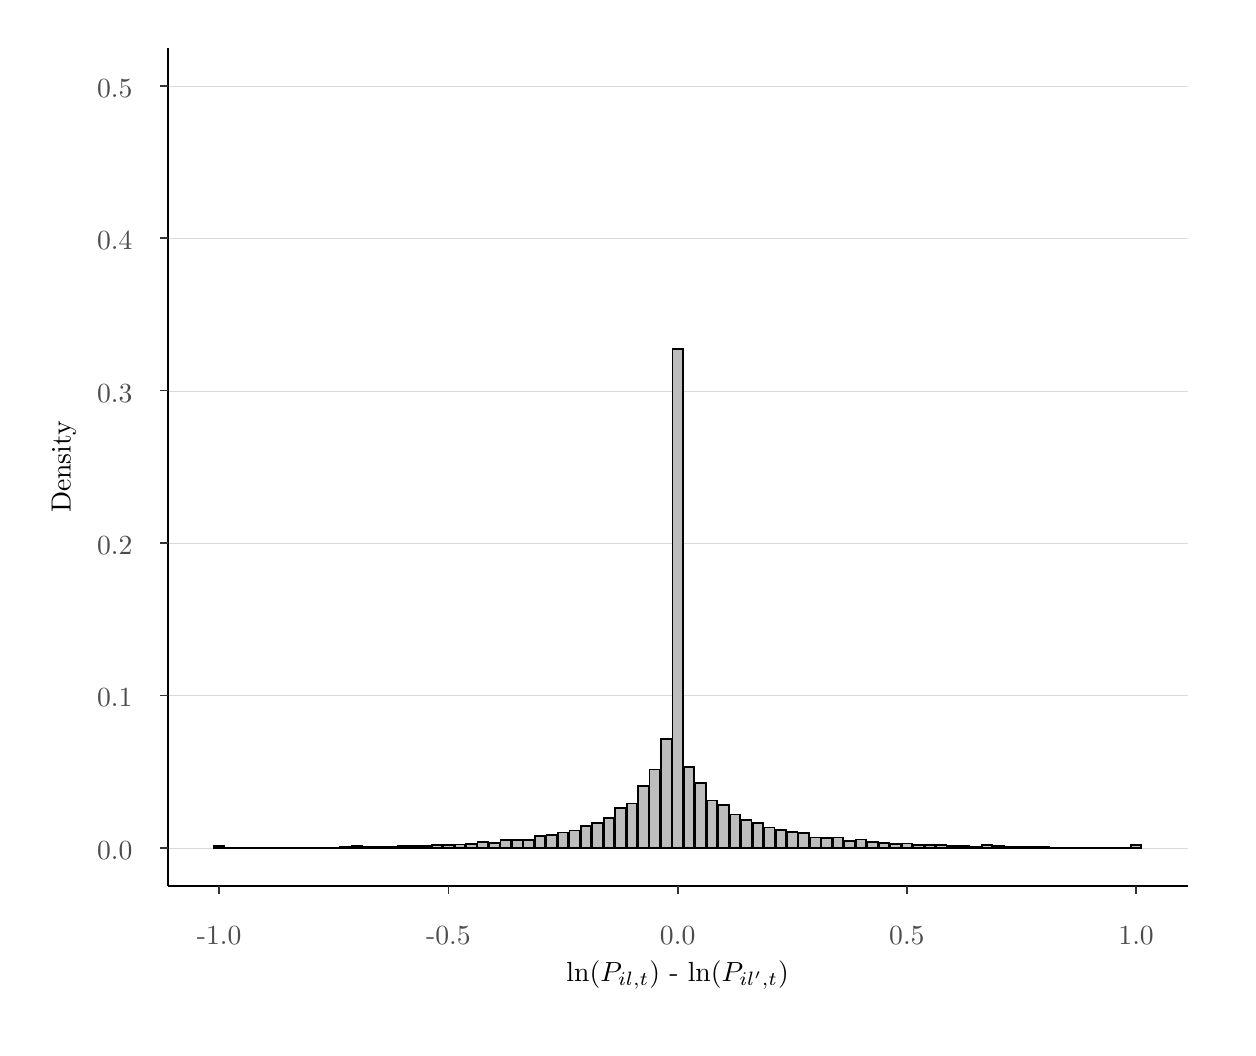
\begin{tikzpicture}[x=1pt,y=1pt]
\definecolor{fillColor}{RGB}{255,255,255}
\path[use as bounding box,fill=fillColor,fill opacity=0.00] (0,0) rectangle (433.62,361.35);
\begin{scope}
\path[clip] (  0.00,  0.00) rectangle (433.62,361.35);
\definecolor{drawColor}{RGB}{255,255,255}
\definecolor{fillColor}{RGB}{255,255,255}

\path[draw=drawColor,line width= 0.6pt,line join=round,line cap=round,fill=fillColor] (  0.00,  0.00) rectangle (433.62,361.35);
\end{scope}
\begin{scope}
\path[clip] ( 50.59, 51.15) rectangle (419.17,354.12);
\definecolor{drawColor}{RGB}{255,255,255}

\path[draw=drawColor,line width= 0.3pt,line join=round] ( 50.59, 92.47) --
	(419.17, 92.47);

\path[draw=drawColor,line width= 0.3pt,line join=round] ( 50.59,147.55) --
	(419.17,147.55);

\path[draw=drawColor,line width= 0.3pt,line join=round] ( 50.59,202.64) --
	(419.17,202.64);

\path[draw=drawColor,line width= 0.3pt,line join=round] ( 50.59,257.72) --
	(419.17,257.72);

\path[draw=drawColor,line width= 0.3pt,line join=round] ( 50.59,312.81) --
	(419.17,312.81);

\path[draw=drawColor,line width= 0.3pt,line join=round] (110.63, 51.15) --
	(110.63,354.12);

\path[draw=drawColor,line width= 0.3pt,line join=round] (193.46, 51.15) --
	(193.46,354.12);

\path[draw=drawColor,line width= 0.3pt,line join=round] (276.30, 51.15) --
	(276.30,354.12);

\path[draw=drawColor,line width= 0.3pt,line join=round] (359.13, 51.15) --
	(359.13,354.12);
\definecolor{drawColor}{gray}{0.85}

\path[draw=drawColor,line width= 0.1pt,line join=round] ( 50.59, 64.92) --
	(419.17, 64.92);

\path[draw=drawColor,line width= 0.1pt,line join=round] ( 50.59,120.01) --
	(419.17,120.01);

\path[draw=drawColor,line width= 0.1pt,line join=round] ( 50.59,175.10) --
	(419.17,175.10);

\path[draw=drawColor,line width= 0.1pt,line join=round] ( 50.59,230.18) --
	(419.17,230.18);

\path[draw=drawColor,line width= 0.1pt,line join=round] ( 50.59,285.27) --
	(419.17,285.27);

\path[draw=drawColor,line width= 0.1pt,line join=round] ( 50.59,340.35) --
	(419.17,340.35);
\definecolor{drawColor}{RGB}{0,0,0}
\definecolor{fillColor}{gray}{0.74}

\path[draw=drawColor,line width= 0.6pt,line cap=rect,fill=fillColor] ( 67.34, 64.92) rectangle ( 71.07, 65.65);

\path[draw=drawColor,line width= 0.6pt,line cap=rect,fill=fillColor] ( 71.49, 64.92) rectangle ( 75.21, 65.00);

\path[draw=drawColor,line width= 0.6pt,line cap=rect,fill=fillColor] ( 75.63, 64.92) rectangle ( 79.36, 65.01);

\path[draw=drawColor,line width= 0.6pt,line cap=rect,fill=fillColor] ( 79.77, 64.92) rectangle ( 83.50, 65.04);

\path[draw=drawColor,line width= 0.6pt,line cap=rect,fill=fillColor] ( 83.91, 64.92) rectangle ( 87.64, 65.02);

\path[draw=drawColor,line width= 0.6pt,line cap=rect,fill=fillColor] ( 88.05, 64.92) rectangle ( 91.78, 65.05);

\path[draw=drawColor,line width= 0.6pt,line cap=rect,fill=fillColor] ( 92.19, 64.92) rectangle ( 95.92, 65.06);

\path[draw=drawColor,line width= 0.6pt,line cap=rect,fill=fillColor] ( 96.34, 64.92) rectangle (100.06, 65.09);

\path[draw=drawColor,line width= 0.6pt,line cap=rect,fill=fillColor] (100.48, 64.92) rectangle (104.21, 65.11);

\path[draw=drawColor,line width= 0.6pt,line cap=rect,fill=fillColor] (104.62, 64.92) rectangle (108.35, 65.14);

\path[draw=drawColor,line width= 0.6pt,line cap=rect,fill=fillColor] (108.76, 64.92) rectangle (112.49, 65.15);

\path[draw=drawColor,line width= 0.6pt,line cap=rect,fill=fillColor] (112.90, 64.92) rectangle (116.63, 65.34);

\path[draw=drawColor,line width= 0.6pt,line cap=rect,fill=fillColor] (117.05, 64.92) rectangle (120.77, 65.71);

\path[draw=drawColor,line width= 0.6pt,line cap=rect,fill=fillColor] (121.19, 64.92) rectangle (124.91, 65.30);

\path[draw=drawColor,line width= 0.6pt,line cap=rect,fill=fillColor] (125.33, 64.92) rectangle (129.06, 65.44);

\path[draw=drawColor,line width= 0.6pt,line cap=rect,fill=fillColor] (129.47, 64.92) rectangle (133.20, 65.38);

\path[draw=drawColor,line width= 0.6pt,line cap=rect,fill=fillColor] (133.61, 64.92) rectangle (137.34, 65.67);

\path[draw=drawColor,line width= 0.6pt,line cap=rect,fill=fillColor] (137.75, 64.92) rectangle (141.48, 65.61);

\path[draw=drawColor,line width= 0.6pt,line cap=rect,fill=fillColor] (141.90, 64.92) rectangle (145.62, 65.70);

\path[draw=drawColor,line width= 0.6pt,line cap=rect,fill=fillColor] (146.04, 64.92) rectangle (149.77, 66.03);

\path[draw=drawColor,line width= 0.6pt,line cap=rect,fill=fillColor] (150.18, 64.92) rectangle (153.91, 65.97);

\path[draw=drawColor,line width= 0.6pt,line cap=rect,fill=fillColor] (154.32, 64.92) rectangle (158.05, 66.19);

\path[draw=drawColor,line width= 0.6pt,line cap=rect,fill=fillColor] (158.46, 64.92) rectangle (162.19, 66.37);

\path[draw=drawColor,line width= 0.6pt,line cap=rect,fill=fillColor] (162.60, 64.92) rectangle (166.33, 67.17);

\path[draw=drawColor,line width= 0.6pt,line cap=rect,fill=fillColor] (166.75, 64.92) rectangle (170.47, 66.80);

\path[draw=drawColor,line width= 0.6pt,line cap=rect,fill=fillColor] (170.89, 64.92) rectangle (174.62, 67.93);

\path[draw=drawColor,line width= 0.6pt,line cap=rect,fill=fillColor] (175.03, 64.92) rectangle (178.76, 67.76);

\path[draw=drawColor,line width= 0.6pt,line cap=rect,fill=fillColor] (179.17, 64.92) rectangle (182.90, 67.90);

\path[draw=drawColor,line width= 0.6pt,line cap=rect,fill=fillColor] (183.31, 64.92) rectangle (187.04, 69.37);

\path[draw=drawColor,line width= 0.6pt,line cap=rect,fill=fillColor] (187.46, 64.92) rectangle (191.18, 69.67);

\path[draw=drawColor,line width= 0.6pt,line cap=rect,fill=fillColor] (191.60, 64.92) rectangle (195.32, 70.49);

\path[draw=drawColor,line width= 0.6pt,line cap=rect,fill=fillColor] (195.74, 64.92) rectangle (199.47, 71.23);

\path[draw=drawColor,line width= 0.6pt,line cap=rect,fill=fillColor] (199.88, 64.92) rectangle (203.61, 72.88);

\path[draw=drawColor,line width= 0.6pt,line cap=rect,fill=fillColor] (204.02, 64.92) rectangle (207.75, 74.02);

\path[draw=drawColor,line width= 0.6pt,line cap=rect,fill=fillColor] (208.16, 64.92) rectangle (211.89, 75.87);

\path[draw=drawColor,line width= 0.6pt,line cap=rect,fill=fillColor] (212.31, 64.92) rectangle (216.03, 79.43);

\path[draw=drawColor,line width= 0.6pt,line cap=rect,fill=fillColor] (216.45, 64.92) rectangle (220.18, 81.02);

\path[draw=drawColor,line width= 0.6pt,line cap=rect,fill=fillColor] (220.59, 64.92) rectangle (224.32, 87.31);

\path[draw=drawColor,line width= 0.6pt,line cap=rect,fill=fillColor] (224.73, 64.92) rectangle (228.46, 93.24);

\path[draw=drawColor,line width= 0.6pt,line cap=rect,fill=fillColor] (228.87, 64.92) rectangle (232.60,104.33);

\path[draw=drawColor,line width= 0.6pt,line cap=rect,fill=fillColor] (233.01, 64.92) rectangle (236.74,245.19);

\path[draw=drawColor,line width= 0.6pt,line cap=rect,fill=fillColor] (237.16, 64.92) rectangle (240.88, 94.11);

\path[draw=drawColor,line width= 0.6pt,line cap=rect,fill=fillColor] (241.30, 64.92) rectangle (245.03, 88.48);

\path[draw=drawColor,line width= 0.6pt,line cap=rect,fill=fillColor] (245.44, 64.92) rectangle (249.17, 82.04);

\path[draw=drawColor,line width= 0.6pt,line cap=rect,fill=fillColor] (249.58, 64.92) rectangle (253.31, 80.55);

\path[draw=drawColor,line width= 0.6pt,line cap=rect,fill=fillColor] (253.72, 64.92) rectangle (257.45, 77.05);

\path[draw=drawColor,line width= 0.6pt,line cap=rect,fill=fillColor] (257.87, 64.92) rectangle (261.59, 75.10);

\path[draw=drawColor,line width= 0.6pt,line cap=rect,fill=fillColor] (262.01, 64.92) rectangle (265.73, 73.95);

\path[draw=drawColor,line width= 0.6pt,line cap=rect,fill=fillColor] (266.15, 64.92) rectangle (269.88, 72.35);

\path[draw=drawColor,line width= 0.6pt,line cap=rect,fill=fillColor] (270.29, 64.92) rectangle (274.02, 71.51);

\path[draw=drawColor,line width= 0.6pt,line cap=rect,fill=fillColor] (274.43, 64.92) rectangle (278.16, 70.77);

\path[draw=drawColor,line width= 0.6pt,line cap=rect,fill=fillColor] (278.57, 64.92) rectangle (282.30, 70.38);

\path[draw=drawColor,line width= 0.6pt,line cap=rect,fill=fillColor] (282.72, 64.92) rectangle (286.44, 68.76);

\path[draw=drawColor,line width= 0.6pt,line cap=rect,fill=fillColor] (286.86, 64.92) rectangle (290.59, 68.56);

\path[draw=drawColor,line width= 0.6pt,line cap=rect,fill=fillColor] (291.00, 64.92) rectangle (294.73, 68.67);

\path[draw=drawColor,line width= 0.6pt,line cap=rect,fill=fillColor] (295.14, 64.92) rectangle (298.87, 67.41);

\path[draw=drawColor,line width= 0.6pt,line cap=rect,fill=fillColor] (299.28, 64.92) rectangle (303.01, 67.96);

\path[draw=drawColor,line width= 0.6pt,line cap=rect,fill=fillColor] (303.42, 64.92) rectangle (307.15, 66.98);

\path[draw=drawColor,line width= 0.6pt,line cap=rect,fill=fillColor] (307.57, 64.92) rectangle (311.29, 66.73);

\path[draw=drawColor,line width= 0.6pt,line cap=rect,fill=fillColor] (311.71, 64.92) rectangle (315.44, 66.44);

\path[draw=drawColor,line width= 0.6pt,line cap=rect,fill=fillColor] (315.85, 64.92) rectangle (319.58, 66.53);

\path[draw=drawColor,line width= 0.6pt,line cap=rect,fill=fillColor] (319.99, 64.92) rectangle (323.72, 66.07);

\path[draw=drawColor,line width= 0.6pt,line cap=rect,fill=fillColor] (324.13, 64.92) rectangle (327.86, 65.94);

\path[draw=drawColor,line width= 0.6pt,line cap=rect,fill=fillColor] (328.28, 64.92) rectangle (332.00, 66.03);

\path[draw=drawColor,line width= 0.6pt,line cap=rect,fill=fillColor] (332.42, 64.92) rectangle (336.14, 65.62);

\path[draw=drawColor,line width= 0.6pt,line cap=rect,fill=fillColor] (336.56, 64.92) rectangle (340.29, 65.67);

\path[draw=drawColor,line width= 0.6pt,line cap=rect,fill=fillColor] (340.70, 64.92) rectangle (344.43, 65.49);

\path[draw=drawColor,line width= 0.6pt,line cap=rect,fill=fillColor] (344.84, 64.92) rectangle (348.57, 65.97);

\path[draw=drawColor,line width= 0.6pt,line cap=rect,fill=fillColor] (348.98, 64.92) rectangle (352.71, 65.53);

\path[draw=drawColor,line width= 0.6pt,line cap=rect,fill=fillColor] (353.13, 64.92) rectangle (356.85, 65.29);

\path[draw=drawColor,line width= 0.6pt,line cap=rect,fill=fillColor] (357.27, 64.92) rectangle (360.99, 65.28);

\path[draw=drawColor,line width= 0.6pt,line cap=rect,fill=fillColor] (361.41, 64.92) rectangle (365.14, 65.23);

\path[draw=drawColor,line width= 0.6pt,line cap=rect,fill=fillColor] (365.55, 64.92) rectangle (369.28, 65.19);

\path[draw=drawColor,line width= 0.6pt,line cap=rect,fill=fillColor] (369.69, 64.92) rectangle (373.42, 65.15);

\path[draw=drawColor,line width= 0.6pt,line cap=rect,fill=fillColor] (373.83, 64.92) rectangle (377.56, 65.14);

\path[draw=drawColor,line width= 0.6pt,line cap=rect,fill=fillColor] (377.98, 64.92) rectangle (381.70, 65.09);

\path[draw=drawColor,line width= 0.6pt,line cap=rect,fill=fillColor] (382.12, 64.92) rectangle (385.85, 65.09);

\path[draw=drawColor,line width= 0.6pt,line cap=rect,fill=fillColor] (386.26, 64.92) rectangle (389.99, 65.06);

\path[draw=drawColor,line width= 0.6pt,line cap=rect,fill=fillColor] (390.40, 64.92) rectangle (394.13, 65.04);

\path[draw=drawColor,line width= 0.6pt,line cap=rect,fill=fillColor] (394.54, 64.92) rectangle (398.27, 65.03);

\path[draw=drawColor,line width= 0.6pt,line cap=rect,fill=fillColor] (398.68, 64.92) rectangle (402.41, 65.95);
\end{scope}
\begin{scope}
\path[clip] (  0.00,  0.00) rectangle (433.62,361.35);
\definecolor{drawColor}{RGB}{0,0,0}

\path[draw=drawColor,line width= 0.6pt,line join=round] ( 50.59, 51.15) --
	( 50.59,354.12);
\end{scope}
\begin{scope}
\path[clip] (  0.00,  0.00) rectangle (433.62,361.35);
\definecolor{drawColor}{gray}{0.30}

\node[text=drawColor,anchor=base east,inner sep=0pt, outer sep=0pt, scale=  1.00] at ( 37.84, 60.79) {0.0};

\node[text=drawColor,anchor=base east,inner sep=0pt, outer sep=0pt, scale=  1.00] at ( 37.84,115.88) {0.1};

\node[text=drawColor,anchor=base east,inner sep=0pt, outer sep=0pt, scale=  1.00] at ( 37.84,170.96) {0.2};

\node[text=drawColor,anchor=base east,inner sep=0pt, outer sep=0pt, scale=  1.00] at ( 37.84,226.05) {0.3};

\node[text=drawColor,anchor=base east,inner sep=0pt, outer sep=0pt, scale=  1.00] at ( 37.84,281.13) {0.4};

\node[text=drawColor,anchor=base east,inner sep=0pt, outer sep=0pt, scale=  1.00] at ( 37.84,336.22) {0.5};
\end{scope}
\begin{scope}
\path[clip] (  0.00,  0.00) rectangle (433.62,361.35);
\definecolor{drawColor}{gray}{0.20}

\path[draw=drawColor,line width= 0.6pt,line join=round] ( 47.84, 64.92) --
	( 50.59, 64.92);

\path[draw=drawColor,line width= 0.6pt,line join=round] ( 47.84,120.01) --
	( 50.59,120.01);

\path[draw=drawColor,line width= 0.6pt,line join=round] ( 47.84,175.10) --
	( 50.59,175.10);

\path[draw=drawColor,line width= 0.6pt,line join=round] ( 47.84,230.18) --
	( 50.59,230.18);

\path[draw=drawColor,line width= 0.6pt,line join=round] ( 47.84,285.27) --
	( 50.59,285.27);

\path[draw=drawColor,line width= 0.6pt,line join=round] ( 47.84,340.35) --
	( 50.59,340.35);
\end{scope}
\begin{scope}
\path[clip] (  0.00,  0.00) rectangle (433.62,361.35);
\definecolor{drawColor}{RGB}{0,0,0}

\path[draw=drawColor,line width= 0.6pt,line join=round] ( 50.59, 51.15) --
	(419.17, 51.15);
\end{scope}
\begin{scope}
\path[clip] (  0.00,  0.00) rectangle (433.62,361.35);
\definecolor{drawColor}{gray}{0.20}

\path[draw=drawColor,line width= 0.6pt,line join=round] ( 69.21, 48.40) --
	( 69.21, 51.15);

\path[draw=drawColor,line width= 0.6pt,line join=round] (152.04, 48.40) --
	(152.04, 51.15);

\path[draw=drawColor,line width= 0.6pt,line join=round] (234.88, 48.40) --
	(234.88, 51.15);

\path[draw=drawColor,line width= 0.6pt,line join=round] (317.71, 48.40) --
	(317.71, 51.15);

\path[draw=drawColor,line width= 0.6pt,line join=round] (400.55, 48.40) --
	(400.55, 51.15);
\end{scope}
\begin{scope}
\path[clip] (  0.00,  0.00) rectangle (433.62,361.35);
\definecolor{drawColor}{gray}{0.30}

\node[text=drawColor,anchor=base,inner sep=0pt, outer sep=0pt, scale=  1.00] at ( 69.21, 30.14) {-1.0};

\node[text=drawColor,anchor=base,inner sep=0pt, outer sep=0pt, scale=  1.00] at (152.04, 30.14) {-0.5};

\node[text=drawColor,anchor=base,inner sep=0pt, outer sep=0pt, scale=  1.00] at (234.88, 30.14) {0.0};

\node[text=drawColor,anchor=base,inner sep=0pt, outer sep=0pt, scale=  1.00] at (317.71, 30.14) {0.5};

\node[text=drawColor,anchor=base,inner sep=0pt, outer sep=0pt, scale=  1.00] at (400.55, 30.14) {1.0};
\end{scope}
\begin{scope}
\path[clip] (  0.00,  0.00) rectangle (433.62,361.35);
\definecolor{drawColor}{RGB}{0,0,0}

\node[text=drawColor,anchor=base,inner sep=0pt, outer sep=0pt, scale=  1.00] at (234.88, 16.79) {ln$\left(P_{il,t}\right)$ - ln$\left(P_{il',t}\right)$};
\end{scope}
\begin{scope}
\path[clip] (  0.00,  0.00) rectangle (433.62,361.35);
\definecolor{drawColor}{RGB}{0,0,0}

\node[text=drawColor,rotate= 90.00,anchor=base,inner sep=0pt, outer sep=0pt, scale=  1.00] at ( 15.49,202.64) {Density};
\end{scope}
\end{tikzpicture}
}
     \end{subfigure}\\
     \begin{subfigure}[t]{.49\textwidth}
         \centering
         \caption{Within store types}
         \label{fig: app_redform_dp_unw_s}
         \scalebox{0.45}{\input{figures/descriptives/P1_2_3_2_1_dp_nr_s.tex}}
     \end{subfigure}
     \begin{subfigure}[t]{.49\textwidth}
         \centering
         \caption{Within household-store types}
         \label{fig: app_redform_dp_unw_hs}
         \scalebox{0.45}{\input{figures/descriptives/P1_2_3_2_1_dp_nr_hs.tex}}
     \end{subfigure}
     \parbox{\textwidth}{
        \begin{spacing}{1} 
            {\footnotesize 
            \textit{Notes}: These figures plot the distribution of LOP deviations across observations at the product variety-NUTS1 pair-year level. Panel (a) pools across stores and household types when computing the LOP deviations. Hence, when computing the price of a product variety in a certain region, we average across stores and household types. Panel (b) and (c) compute LOP deviations within household and store types respectively. Panel (d) computes LOP deviations within store types and household types. The distributions are based on simple counts per bin.}
        \end{spacing}}
 \end{figure} 

 \begin{figure}[H]
    \centering
    \caption{LOP deviations - Transaction weighted}
    \label{fig: app_redform_dp_w}
    \begin{subfigure}[t]{.49\textwidth}
         \centering
         \caption{Pooled}
         \scalebox{0.45}{% Created by tikzDevice version 0.12.3.1 on 2022-10-03 20:25:19
% !TEX encoding = UTF-8 Unicode
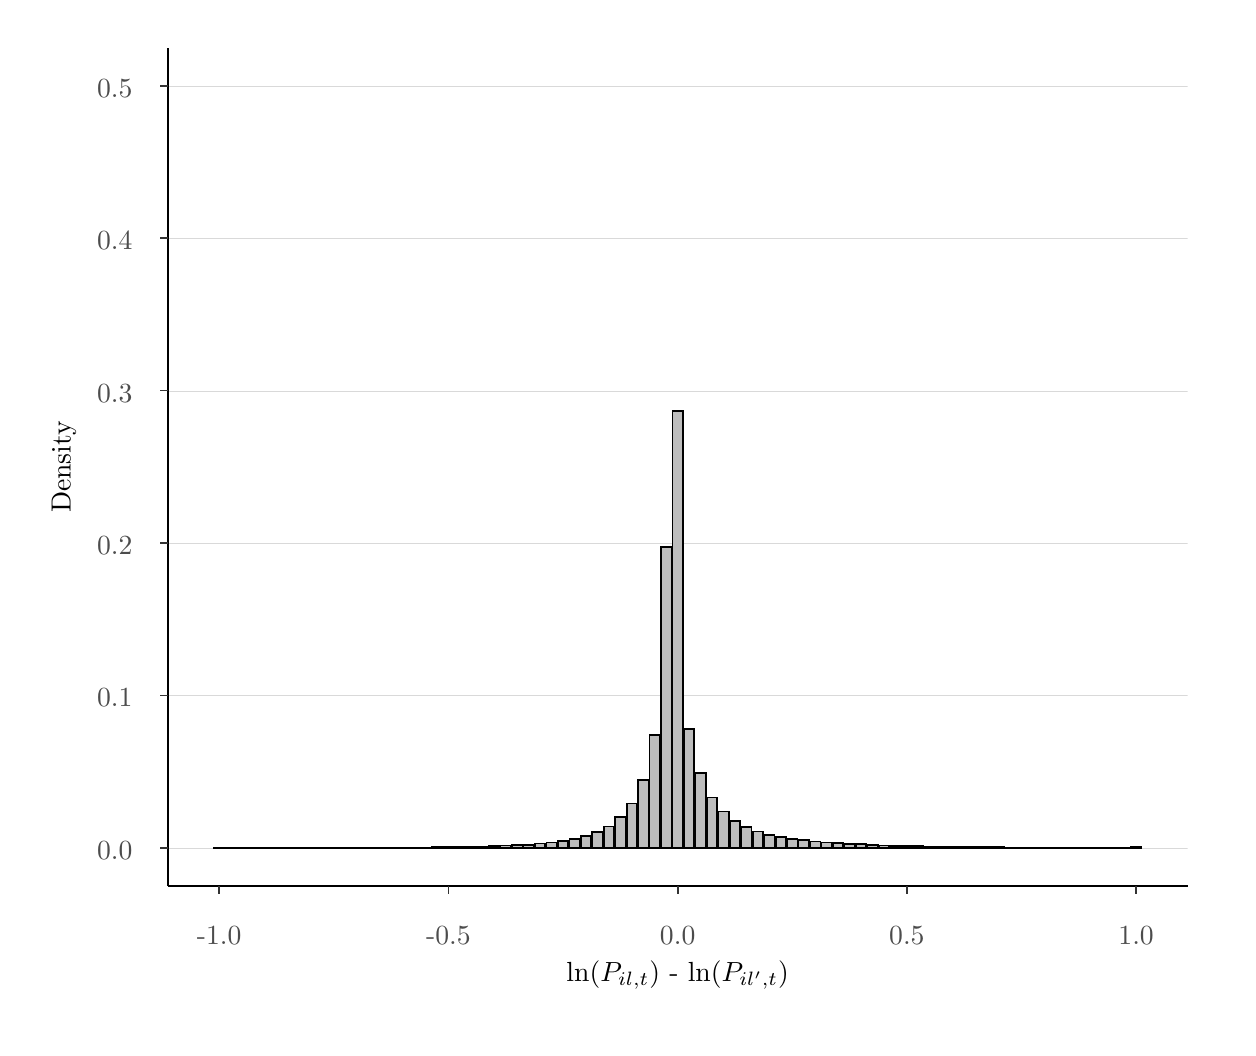
\begin{tikzpicture}[x=1pt,y=1pt]
\definecolor{fillColor}{RGB}{255,255,255}
\path[use as bounding box,fill=fillColor,fill opacity=0.00] (0,0) rectangle (433.62,361.35);
\begin{scope}
\path[clip] (  0.00,  0.00) rectangle (433.62,361.35);
\definecolor{drawColor}{RGB}{255,255,255}
\definecolor{fillColor}{RGB}{255,255,255}

\path[draw=drawColor,line width= 0.6pt,line join=round,line cap=round,fill=fillColor] (  0.00,  0.00) rectangle (433.62,361.35);
\end{scope}
\begin{scope}
\path[clip] ( 50.59, 51.15) rectangle (419.17,354.12);
\definecolor{drawColor}{RGB}{255,255,255}

\path[draw=drawColor,line width= 0.3pt,line join=round] ( 50.59, 92.47) --
	(419.17, 92.47);

\path[draw=drawColor,line width= 0.3pt,line join=round] ( 50.59,147.55) --
	(419.17,147.55);

\path[draw=drawColor,line width= 0.3pt,line join=round] ( 50.59,202.64) --
	(419.17,202.64);

\path[draw=drawColor,line width= 0.3pt,line join=round] ( 50.59,257.72) --
	(419.17,257.72);

\path[draw=drawColor,line width= 0.3pt,line join=round] ( 50.59,312.81) --
	(419.17,312.81);

\path[draw=drawColor,line width= 0.3pt,line join=round] (110.63, 51.15) --
	(110.63,354.12);

\path[draw=drawColor,line width= 0.3pt,line join=round] (193.46, 51.15) --
	(193.46,354.12);

\path[draw=drawColor,line width= 0.3pt,line join=round] (276.30, 51.15) --
	(276.30,354.12);

\path[draw=drawColor,line width= 0.3pt,line join=round] (359.13, 51.15) --
	(359.13,354.12);
\definecolor{drawColor}{gray}{0.85}

\path[draw=drawColor,line width= 0.1pt,line join=round] ( 50.59, 64.92) --
	(419.17, 64.92);

\path[draw=drawColor,line width= 0.1pt,line join=round] ( 50.59,120.01) --
	(419.17,120.01);

\path[draw=drawColor,line width= 0.1pt,line join=round] ( 50.59,175.10) --
	(419.17,175.10);

\path[draw=drawColor,line width= 0.1pt,line join=round] ( 50.59,230.18) --
	(419.17,230.18);

\path[draw=drawColor,line width= 0.1pt,line join=round] ( 50.59,285.27) --
	(419.17,285.27);

\path[draw=drawColor,line width= 0.1pt,line join=round] ( 50.59,340.35) --
	(419.17,340.35);
\definecolor{drawColor}{RGB}{0,0,0}
\definecolor{fillColor}{gray}{0.74}

\path[draw=drawColor,line width= 0.6pt,line cap=rect,fill=fillColor] ( 67.34, 64.92) rectangle ( 71.07, 65.15);

\path[draw=drawColor,line width= 0.6pt,line cap=rect,fill=fillColor] ( 71.49, 64.92) rectangle ( 75.21, 64.94);

\path[draw=drawColor,line width= 0.6pt,line cap=rect,fill=fillColor] ( 75.63, 64.92) rectangle ( 79.36, 64.94);

\path[draw=drawColor,line width= 0.6pt,line cap=rect,fill=fillColor] ( 79.77, 64.92) rectangle ( 83.50, 64.95);

\path[draw=drawColor,line width= 0.6pt,line cap=rect,fill=fillColor] ( 83.91, 64.92) rectangle ( 87.64, 64.95);

\path[draw=drawColor,line width= 0.6pt,line cap=rect,fill=fillColor] ( 88.05, 64.92) rectangle ( 91.78, 64.95);

\path[draw=drawColor,line width= 0.6pt,line cap=rect,fill=fillColor] ( 92.19, 64.92) rectangle ( 95.92, 64.96);

\path[draw=drawColor,line width= 0.6pt,line cap=rect,fill=fillColor] ( 96.34, 64.92) rectangle (100.06, 64.96);

\path[draw=drawColor,line width= 0.6pt,line cap=rect,fill=fillColor] (100.48, 64.92) rectangle (104.21, 64.97);

\path[draw=drawColor,line width= 0.6pt,line cap=rect,fill=fillColor] (104.62, 64.92) rectangle (108.35, 64.97);

\path[draw=drawColor,line width= 0.6pt,line cap=rect,fill=fillColor] (108.76, 64.92) rectangle (112.49, 64.98);

\path[draw=drawColor,line width= 0.6pt,line cap=rect,fill=fillColor] (112.90, 64.92) rectangle (116.63, 65.01);

\path[draw=drawColor,line width= 0.6pt,line cap=rect,fill=fillColor] (117.05, 64.92) rectangle (120.77, 65.06);

\path[draw=drawColor,line width= 0.6pt,line cap=rect,fill=fillColor] (121.19, 64.92) rectangle (124.91, 65.02);

\path[draw=drawColor,line width= 0.6pt,line cap=rect,fill=fillColor] (125.33, 64.92) rectangle (129.06, 65.05);

\path[draw=drawColor,line width= 0.6pt,line cap=rect,fill=fillColor] (129.47, 64.92) rectangle (133.20, 65.06);

\path[draw=drawColor,line width= 0.6pt,line cap=rect,fill=fillColor] (133.61, 64.92) rectangle (137.34, 65.08);

\path[draw=drawColor,line width= 0.6pt,line cap=rect,fill=fillColor] (137.75, 64.92) rectangle (141.48, 65.11);

\path[draw=drawColor,line width= 0.6pt,line cap=rect,fill=fillColor] (141.90, 64.92) rectangle (145.62, 65.14);

\path[draw=drawColor,line width= 0.6pt,line cap=rect,fill=fillColor] (146.04, 64.92) rectangle (149.77, 65.19);

\path[draw=drawColor,line width= 0.6pt,line cap=rect,fill=fillColor] (150.18, 64.92) rectangle (153.91, 65.22);

\path[draw=drawColor,line width= 0.6pt,line cap=rect,fill=fillColor] (154.32, 64.92) rectangle (158.05, 65.28);

\path[draw=drawColor,line width= 0.6pt,line cap=rect,fill=fillColor] (158.46, 64.92) rectangle (162.19, 65.35);

\path[draw=drawColor,line width= 0.6pt,line cap=rect,fill=fillColor] (162.60, 64.92) rectangle (166.33, 65.50);

\path[draw=drawColor,line width= 0.6pt,line cap=rect,fill=fillColor] (166.75, 64.92) rectangle (170.47, 65.56);

\path[draw=drawColor,line width= 0.6pt,line cap=rect,fill=fillColor] (170.89, 64.92) rectangle (174.62, 65.81);

\path[draw=drawColor,line width= 0.6pt,line cap=rect,fill=fillColor] (175.03, 64.92) rectangle (178.76, 65.95);

\path[draw=drawColor,line width= 0.6pt,line cap=rect,fill=fillColor] (179.17, 64.92) rectangle (182.90, 66.12);

\path[draw=drawColor,line width= 0.6pt,line cap=rect,fill=fillColor] (183.31, 64.92) rectangle (187.04, 66.52);

\path[draw=drawColor,line width= 0.6pt,line cap=rect,fill=fillColor] (187.46, 64.92) rectangle (191.18, 66.86);

\path[draw=drawColor,line width= 0.6pt,line cap=rect,fill=fillColor] (191.60, 64.92) rectangle (195.32, 67.46);

\path[draw=drawColor,line width= 0.6pt,line cap=rect,fill=fillColor] (195.74, 64.92) rectangle (199.47, 68.18);

\path[draw=drawColor,line width= 0.6pt,line cap=rect,fill=fillColor] (199.88, 64.92) rectangle (203.61, 69.25);

\path[draw=drawColor,line width= 0.6pt,line cap=rect,fill=fillColor] (204.02, 64.92) rectangle (207.75, 70.69);

\path[draw=drawColor,line width= 0.6pt,line cap=rect,fill=fillColor] (208.16, 64.92) rectangle (211.89, 72.73);

\path[draw=drawColor,line width= 0.6pt,line cap=rect,fill=fillColor] (212.31, 64.92) rectangle (216.03, 76.16);

\path[draw=drawColor,line width= 0.6pt,line cap=rect,fill=fillColor] (216.45, 64.92) rectangle (220.18, 81.00);

\path[draw=drawColor,line width= 0.6pt,line cap=rect,fill=fillColor] (220.59, 64.92) rectangle (224.32, 89.44);

\path[draw=drawColor,line width= 0.6pt,line cap=rect,fill=fillColor] (224.73, 64.92) rectangle (228.46,105.83);

\path[draw=drawColor,line width= 0.6pt,line cap=rect,fill=fillColor] (228.87, 64.92) rectangle (232.60,173.57);

\path[draw=drawColor,line width= 0.6pt,line cap=rect,fill=fillColor] (233.01, 64.92) rectangle (236.74,222.88);

\path[draw=drawColor,line width= 0.6pt,line cap=rect,fill=fillColor] (237.16, 64.92) rectangle (240.88,108.02);

\path[draw=drawColor,line width= 0.6pt,line cap=rect,fill=fillColor] (241.30, 64.92) rectangle (245.03, 91.92);

\path[draw=drawColor,line width= 0.6pt,line cap=rect,fill=fillColor] (245.44, 64.92) rectangle (249.17, 83.14);

\path[draw=drawColor,line width= 0.6pt,line cap=rect,fill=fillColor] (249.58, 64.92) rectangle (253.31, 78.12);

\path[draw=drawColor,line width= 0.6pt,line cap=rect,fill=fillColor] (253.72, 64.92) rectangle (257.45, 74.70);

\path[draw=drawColor,line width= 0.6pt,line cap=rect,fill=fillColor] (257.87, 64.92) rectangle (261.59, 72.41);

\path[draw=drawColor,line width= 0.6pt,line cap=rect,fill=fillColor] (262.01, 64.92) rectangle (265.73, 70.86);

\path[draw=drawColor,line width= 0.6pt,line cap=rect,fill=fillColor] (266.15, 64.92) rectangle (269.88, 69.66);

\path[draw=drawColor,line width= 0.6pt,line cap=rect,fill=fillColor] (270.29, 64.92) rectangle (274.02, 68.91);

\path[draw=drawColor,line width= 0.6pt,line cap=rect,fill=fillColor] (274.43, 64.92) rectangle (278.16, 68.27);

\path[draw=drawColor,line width= 0.6pt,line cap=rect,fill=fillColor] (278.57, 64.92) rectangle (282.30, 67.78);

\path[draw=drawColor,line width= 0.6pt,line cap=rect,fill=fillColor] (282.72, 64.92) rectangle (286.44, 67.27);

\path[draw=drawColor,line width= 0.6pt,line cap=rect,fill=fillColor] (286.86, 64.92) rectangle (290.59, 66.94);

\path[draw=drawColor,line width= 0.6pt,line cap=rect,fill=fillColor] (291.00, 64.92) rectangle (294.73, 66.70);

\path[draw=drawColor,line width= 0.6pt,line cap=rect,fill=fillColor] (295.14, 64.92) rectangle (298.87, 66.34);

\path[draw=drawColor,line width= 0.6pt,line cap=rect,fill=fillColor] (299.28, 64.92) rectangle (303.01, 66.31);

\path[draw=drawColor,line width= 0.6pt,line cap=rect,fill=fillColor] (303.42, 64.92) rectangle (307.15, 66.01);

\path[draw=drawColor,line width= 0.6pt,line cap=rect,fill=fillColor] (307.57, 64.92) rectangle (311.29, 65.87);

\path[draw=drawColor,line width= 0.6pt,line cap=rect,fill=fillColor] (311.71, 64.92) rectangle (315.44, 65.73);

\path[draw=drawColor,line width= 0.6pt,line cap=rect,fill=fillColor] (315.85, 64.92) rectangle (319.58, 65.70);

\path[draw=drawColor,line width= 0.6pt,line cap=rect,fill=fillColor] (319.99, 64.92) rectangle (323.72, 65.54);

\path[draw=drawColor,line width= 0.6pt,line cap=rect,fill=fillColor] (324.13, 64.92) rectangle (327.86, 65.47);

\path[draw=drawColor,line width= 0.6pt,line cap=rect,fill=fillColor] (328.28, 64.92) rectangle (332.00, 65.43);

\path[draw=drawColor,line width= 0.6pt,line cap=rect,fill=fillColor] (332.42, 64.92) rectangle (336.14, 65.30);

\path[draw=drawColor,line width= 0.6pt,line cap=rect,fill=fillColor] (336.56, 64.92) rectangle (340.29, 65.27);

\path[draw=drawColor,line width= 0.6pt,line cap=rect,fill=fillColor] (340.70, 64.92) rectangle (344.43, 65.21);

\path[draw=drawColor,line width= 0.6pt,line cap=rect,fill=fillColor] (344.84, 64.92) rectangle (348.57, 65.28);

\path[draw=drawColor,line width= 0.6pt,line cap=rect,fill=fillColor] (348.98, 64.92) rectangle (352.71, 65.17);

\path[draw=drawColor,line width= 0.6pt,line cap=rect,fill=fillColor] (353.13, 64.92) rectangle (356.85, 65.10);

\path[draw=drawColor,line width= 0.6pt,line cap=rect,fill=fillColor] (357.27, 64.92) rectangle (360.99, 65.08);

\path[draw=drawColor,line width= 0.6pt,line cap=rect,fill=fillColor] (361.41, 64.92) rectangle (365.14, 65.05);

\path[draw=drawColor,line width= 0.6pt,line cap=rect,fill=fillColor] (365.55, 64.92) rectangle (369.28, 65.03);

\path[draw=drawColor,line width= 0.6pt,line cap=rect,fill=fillColor] (369.69, 64.92) rectangle (373.42, 65.02);

\path[draw=drawColor,line width= 0.6pt,line cap=rect,fill=fillColor] (373.83, 64.92) rectangle (377.56, 65.01);

\path[draw=drawColor,line width= 0.6pt,line cap=rect,fill=fillColor] (377.98, 64.92) rectangle (381.70, 64.99);

\path[draw=drawColor,line width= 0.6pt,line cap=rect,fill=fillColor] (382.12, 64.92) rectangle (385.85, 64.98);

\path[draw=drawColor,line width= 0.6pt,line cap=rect,fill=fillColor] (386.26, 64.92) rectangle (389.99, 64.97);

\path[draw=drawColor,line width= 0.6pt,line cap=rect,fill=fillColor] (390.40, 64.92) rectangle (394.13, 64.97);

\path[draw=drawColor,line width= 0.6pt,line cap=rect,fill=fillColor] (394.54, 64.92) rectangle (398.27, 64.96);

\path[draw=drawColor,line width= 0.6pt,line cap=rect,fill=fillColor] (398.68, 64.92) rectangle (402.41, 65.48);
\end{scope}
\begin{scope}
\path[clip] (  0.00,  0.00) rectangle (433.62,361.35);
\definecolor{drawColor}{RGB}{0,0,0}

\path[draw=drawColor,line width= 0.6pt,line join=round] ( 50.59, 51.15) --
	( 50.59,354.12);
\end{scope}
\begin{scope}
\path[clip] (  0.00,  0.00) rectangle (433.62,361.35);
\definecolor{drawColor}{gray}{0.30}

\node[text=drawColor,anchor=base east,inner sep=0pt, outer sep=0pt, scale=  1.00] at ( 37.84, 60.79) {0.0};

\node[text=drawColor,anchor=base east,inner sep=0pt, outer sep=0pt, scale=  1.00] at ( 37.84,115.88) {0.1};

\node[text=drawColor,anchor=base east,inner sep=0pt, outer sep=0pt, scale=  1.00] at ( 37.84,170.96) {0.2};

\node[text=drawColor,anchor=base east,inner sep=0pt, outer sep=0pt, scale=  1.00] at ( 37.84,226.05) {0.3};

\node[text=drawColor,anchor=base east,inner sep=0pt, outer sep=0pt, scale=  1.00] at ( 37.84,281.13) {0.4};

\node[text=drawColor,anchor=base east,inner sep=0pt, outer sep=0pt, scale=  1.00] at ( 37.84,336.22) {0.5};
\end{scope}
\begin{scope}
\path[clip] (  0.00,  0.00) rectangle (433.62,361.35);
\definecolor{drawColor}{gray}{0.20}

\path[draw=drawColor,line width= 0.6pt,line join=round] ( 47.84, 64.92) --
	( 50.59, 64.92);

\path[draw=drawColor,line width= 0.6pt,line join=round] ( 47.84,120.01) --
	( 50.59,120.01);

\path[draw=drawColor,line width= 0.6pt,line join=round] ( 47.84,175.10) --
	( 50.59,175.10);

\path[draw=drawColor,line width= 0.6pt,line join=round] ( 47.84,230.18) --
	( 50.59,230.18);

\path[draw=drawColor,line width= 0.6pt,line join=round] ( 47.84,285.27) --
	( 50.59,285.27);

\path[draw=drawColor,line width= 0.6pt,line join=round] ( 47.84,340.35) --
	( 50.59,340.35);
\end{scope}
\begin{scope}
\path[clip] (  0.00,  0.00) rectangle (433.62,361.35);
\definecolor{drawColor}{RGB}{0,0,0}

\path[draw=drawColor,line width= 0.6pt,line join=round] ( 50.59, 51.15) --
	(419.17, 51.15);
\end{scope}
\begin{scope}
\path[clip] (  0.00,  0.00) rectangle (433.62,361.35);
\definecolor{drawColor}{gray}{0.20}

\path[draw=drawColor,line width= 0.6pt,line join=round] ( 69.21, 48.40) --
	( 69.21, 51.15);

\path[draw=drawColor,line width= 0.6pt,line join=round] (152.04, 48.40) --
	(152.04, 51.15);

\path[draw=drawColor,line width= 0.6pt,line join=round] (234.88, 48.40) --
	(234.88, 51.15);

\path[draw=drawColor,line width= 0.6pt,line join=round] (317.71, 48.40) --
	(317.71, 51.15);

\path[draw=drawColor,line width= 0.6pt,line join=round] (400.55, 48.40) --
	(400.55, 51.15);
\end{scope}
\begin{scope}
\path[clip] (  0.00,  0.00) rectangle (433.62,361.35);
\definecolor{drawColor}{gray}{0.30}

\node[text=drawColor,anchor=base,inner sep=0pt, outer sep=0pt, scale=  1.00] at ( 69.21, 30.14) {-1.0};

\node[text=drawColor,anchor=base,inner sep=0pt, outer sep=0pt, scale=  1.00] at (152.04, 30.14) {-0.5};

\node[text=drawColor,anchor=base,inner sep=0pt, outer sep=0pt, scale=  1.00] at (234.88, 30.14) {0.0};

\node[text=drawColor,anchor=base,inner sep=0pt, outer sep=0pt, scale=  1.00] at (317.71, 30.14) {0.5};

\node[text=drawColor,anchor=base,inner sep=0pt, outer sep=0pt, scale=  1.00] at (400.55, 30.14) {1.0};
\end{scope}
\begin{scope}
\path[clip] (  0.00,  0.00) rectangle (433.62,361.35);
\definecolor{drawColor}{RGB}{0,0,0}

\node[text=drawColor,anchor=base,inner sep=0pt, outer sep=0pt, scale=  1.00] at (234.88, 16.79) {ln$\left(P_{il,t}\right)$ - ln$\left(P_{il',t}\right)$};
\end{scope}
\begin{scope}
\path[clip] (  0.00,  0.00) rectangle (433.62,361.35);
\definecolor{drawColor}{RGB}{0,0,0}

\node[text=drawColor,rotate= 90.00,anchor=base,inner sep=0pt, outer sep=0pt, scale=  1.00] at ( 15.49,202.64) {Density};
\end{scope}
\end{tikzpicture}
}
     \end{subfigure}
     \begin{subfigure}[t]{.49\textwidth}
         \centering
         \caption{Within household types}
         \scalebox{0.45}{\input{figures/descriptives/P1_2_3_2_1_dp_trans_h.tex}}
     \end{subfigure}\\
     \begin{subfigure}[t]{.49\textwidth}
         \centering
         \caption{Within store types}
         \scalebox{0.45}{% Created by tikzDevice version 0.12.3.1 on 2022-10-03 20:25:19
% !TEX encoding = UTF-8 Unicode
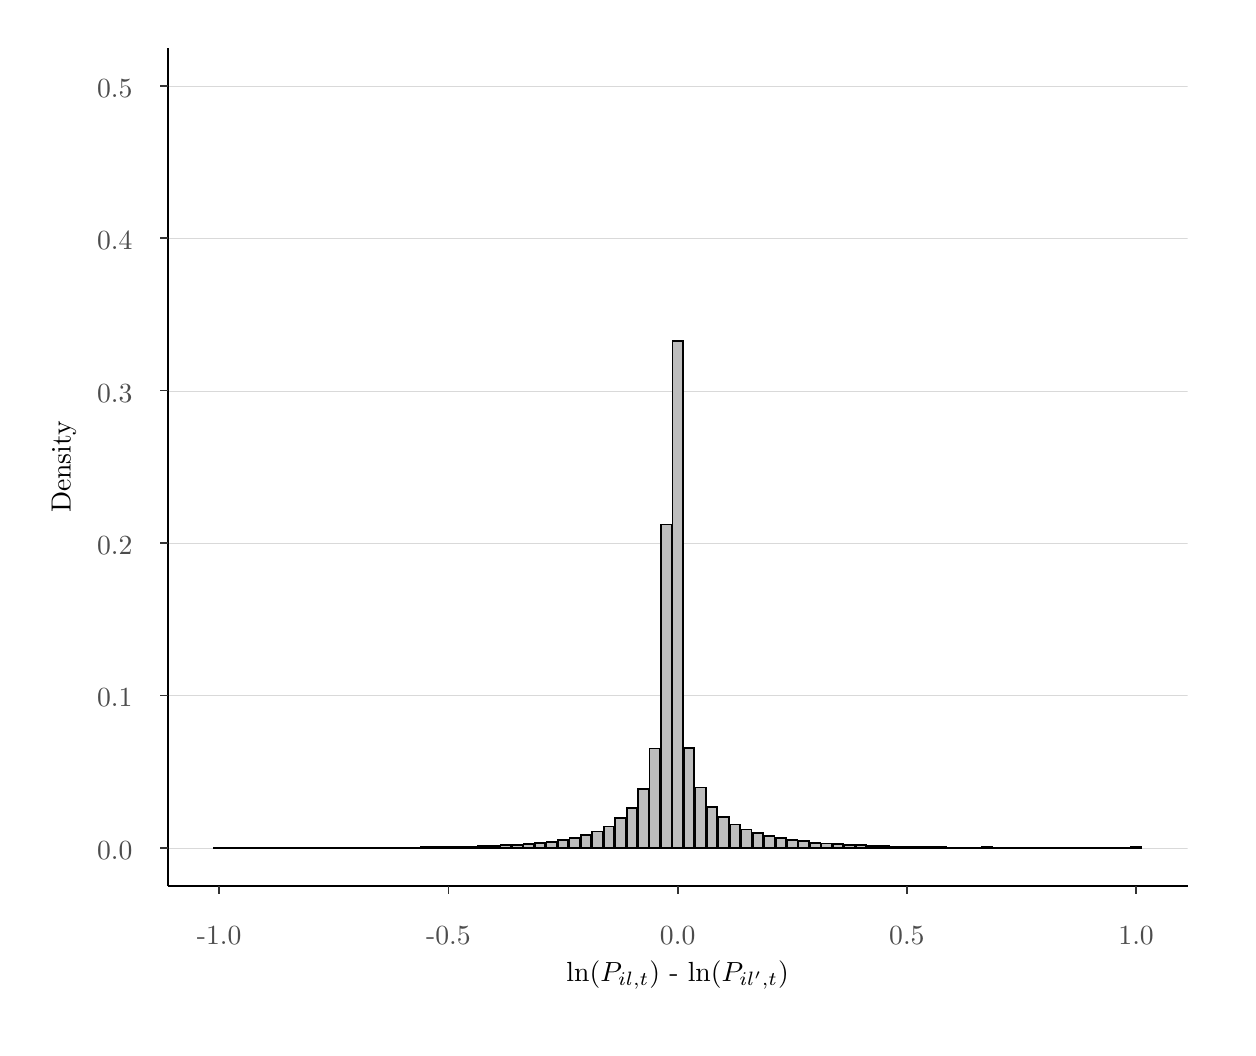
\begin{tikzpicture}[x=1pt,y=1pt]
\definecolor{fillColor}{RGB}{255,255,255}
\path[use as bounding box,fill=fillColor,fill opacity=0.00] (0,0) rectangle (433.62,361.35);
\begin{scope}
\path[clip] (  0.00,  0.00) rectangle (433.62,361.35);
\definecolor{drawColor}{RGB}{255,255,255}
\definecolor{fillColor}{RGB}{255,255,255}

\path[draw=drawColor,line width= 0.6pt,line join=round,line cap=round,fill=fillColor] (  0.00,  0.00) rectangle (433.62,361.35);
\end{scope}
\begin{scope}
\path[clip] ( 50.59, 51.15) rectangle (419.17,354.12);
\definecolor{drawColor}{RGB}{255,255,255}

\path[draw=drawColor,line width= 0.3pt,line join=round] ( 50.59, 92.47) --
	(419.17, 92.47);

\path[draw=drawColor,line width= 0.3pt,line join=round] ( 50.59,147.55) --
	(419.17,147.55);

\path[draw=drawColor,line width= 0.3pt,line join=round] ( 50.59,202.64) --
	(419.17,202.64);

\path[draw=drawColor,line width= 0.3pt,line join=round] ( 50.59,257.72) --
	(419.17,257.72);

\path[draw=drawColor,line width= 0.3pt,line join=round] ( 50.59,312.81) --
	(419.17,312.81);

\path[draw=drawColor,line width= 0.3pt,line join=round] (110.63, 51.15) --
	(110.63,354.12);

\path[draw=drawColor,line width= 0.3pt,line join=round] (193.46, 51.15) --
	(193.46,354.12);

\path[draw=drawColor,line width= 0.3pt,line join=round] (276.30, 51.15) --
	(276.30,354.12);

\path[draw=drawColor,line width= 0.3pt,line join=round] (359.13, 51.15) --
	(359.13,354.12);
\definecolor{drawColor}{gray}{0.85}

\path[draw=drawColor,line width= 0.1pt,line join=round] ( 50.59, 64.92) --
	(419.17, 64.92);

\path[draw=drawColor,line width= 0.1pt,line join=round] ( 50.59,120.01) --
	(419.17,120.01);

\path[draw=drawColor,line width= 0.1pt,line join=round] ( 50.59,175.10) --
	(419.17,175.10);

\path[draw=drawColor,line width= 0.1pt,line join=round] ( 50.59,230.18) --
	(419.17,230.18);

\path[draw=drawColor,line width= 0.1pt,line join=round] ( 50.59,285.27) --
	(419.17,285.27);

\path[draw=drawColor,line width= 0.1pt,line join=round] ( 50.59,340.35) --
	(419.17,340.35);
\definecolor{drawColor}{RGB}{0,0,0}
\definecolor{fillColor}{gray}{0.74}

\path[draw=drawColor,line width= 0.6pt,line cap=rect,fill=fillColor] ( 67.34, 64.92) rectangle ( 71.07, 65.13);

\path[draw=drawColor,line width= 0.6pt,line cap=rect,fill=fillColor] ( 71.49, 64.92) rectangle ( 75.21, 64.94);

\path[draw=drawColor,line width= 0.6pt,line cap=rect,fill=fillColor] ( 75.63, 64.92) rectangle ( 79.36, 64.95);

\path[draw=drawColor,line width= 0.6pt,line cap=rect,fill=fillColor] ( 79.77, 64.92) rectangle ( 83.50, 64.95);

\path[draw=drawColor,line width= 0.6pt,line cap=rect,fill=fillColor] ( 83.91, 64.92) rectangle ( 87.64, 64.95);

\path[draw=drawColor,line width= 0.6pt,line cap=rect,fill=fillColor] ( 88.05, 64.92) rectangle ( 91.78, 64.96);

\path[draw=drawColor,line width= 0.6pt,line cap=rect,fill=fillColor] ( 92.19, 64.92) rectangle ( 95.92, 64.97);

\path[draw=drawColor,line width= 0.6pt,line cap=rect,fill=fillColor] ( 96.34, 64.92) rectangle (100.06, 64.97);

\path[draw=drawColor,line width= 0.6pt,line cap=rect,fill=fillColor] (100.48, 64.92) rectangle (104.21, 64.98);

\path[draw=drawColor,line width= 0.6pt,line cap=rect,fill=fillColor] (104.62, 64.92) rectangle (108.35, 64.98);

\path[draw=drawColor,line width= 0.6pt,line cap=rect,fill=fillColor] (108.76, 64.92) rectangle (112.49, 64.99);

\path[draw=drawColor,line width= 0.6pt,line cap=rect,fill=fillColor] (112.90, 64.92) rectangle (116.63, 65.03);

\path[draw=drawColor,line width= 0.6pt,line cap=rect,fill=fillColor] (117.05, 64.92) rectangle (120.77, 65.11);

\path[draw=drawColor,line width= 0.6pt,line cap=rect,fill=fillColor] (121.19, 64.92) rectangle (124.91, 65.04);

\path[draw=drawColor,line width= 0.6pt,line cap=rect,fill=fillColor] (125.33, 64.92) rectangle (129.06, 65.07);

\path[draw=drawColor,line width= 0.6pt,line cap=rect,fill=fillColor] (129.47, 64.92) rectangle (133.20, 65.08);

\path[draw=drawColor,line width= 0.6pt,line cap=rect,fill=fillColor] (133.61, 64.92) rectangle (137.34, 65.12);

\path[draw=drawColor,line width= 0.6pt,line cap=rect,fill=fillColor] (137.75, 64.92) rectangle (141.48, 65.15);

\path[draw=drawColor,line width= 0.6pt,line cap=rect,fill=fillColor] (141.90, 64.92) rectangle (145.62, 65.17);

\path[draw=drawColor,line width= 0.6pt,line cap=rect,fill=fillColor] (146.04, 64.92) rectangle (149.77, 65.25);

\path[draw=drawColor,line width= 0.6pt,line cap=rect,fill=fillColor] (150.18, 64.92) rectangle (153.91, 65.26);

\path[draw=drawColor,line width= 0.6pt,line cap=rect,fill=fillColor] (154.32, 64.92) rectangle (158.05, 65.34);

\path[draw=drawColor,line width= 0.6pt,line cap=rect,fill=fillColor] (158.46, 64.92) rectangle (162.19, 65.42);

\path[draw=drawColor,line width= 0.6pt,line cap=rect,fill=fillColor] (162.60, 64.92) rectangle (166.33, 65.63);

\path[draw=drawColor,line width= 0.6pt,line cap=rect,fill=fillColor] (166.75, 64.92) rectangle (170.47, 65.67);

\path[draw=drawColor,line width= 0.6pt,line cap=rect,fill=fillColor] (170.89, 64.92) rectangle (174.62, 65.98);

\path[draw=drawColor,line width= 0.6pt,line cap=rect,fill=fillColor] (175.03, 64.92) rectangle (178.76, 66.12);

\path[draw=drawColor,line width= 0.6pt,line cap=rect,fill=fillColor] (179.17, 64.92) rectangle (182.90, 66.33);

\path[draw=drawColor,line width= 0.6pt,line cap=rect,fill=fillColor] (183.31, 64.92) rectangle (187.04, 66.84);

\path[draw=drawColor,line width= 0.6pt,line cap=rect,fill=fillColor] (187.46, 64.92) rectangle (191.18, 67.18);

\path[draw=drawColor,line width= 0.6pt,line cap=rect,fill=fillColor] (191.60, 64.92) rectangle (195.32, 67.81);

\path[draw=drawColor,line width= 0.6pt,line cap=rect,fill=fillColor] (195.74, 64.92) rectangle (199.47, 68.55);

\path[draw=drawColor,line width= 0.6pt,line cap=rect,fill=fillColor] (199.88, 64.92) rectangle (203.61, 69.62);

\path[draw=drawColor,line width= 0.6pt,line cap=rect,fill=fillColor] (204.02, 64.92) rectangle (207.75, 70.94);

\path[draw=drawColor,line width= 0.6pt,line cap=rect,fill=fillColor] (208.16, 64.92) rectangle (211.89, 72.66);

\path[draw=drawColor,line width= 0.6pt,line cap=rect,fill=fillColor] (212.31, 64.92) rectangle (216.03, 75.66);

\path[draw=drawColor,line width= 0.6pt,line cap=rect,fill=fillColor] (216.45, 64.92) rectangle (220.18, 79.27);

\path[draw=drawColor,line width= 0.6pt,line cap=rect,fill=fillColor] (220.59, 64.92) rectangle (224.32, 86.23);

\path[draw=drawColor,line width= 0.6pt,line cap=rect,fill=fillColor] (224.73, 64.92) rectangle (228.46,100.86);

\path[draw=drawColor,line width= 0.6pt,line cap=rect,fill=fillColor] (228.87, 64.92) rectangle (232.60,181.88);

\path[draw=drawColor,line width= 0.6pt,line cap=rect,fill=fillColor] (233.01, 64.92) rectangle (236.74,248.23);

\path[draw=drawColor,line width= 0.6pt,line cap=rect,fill=fillColor] (237.16, 64.92) rectangle (240.88,101.02);

\path[draw=drawColor,line width= 0.6pt,line cap=rect,fill=fillColor] (241.30, 64.92) rectangle (245.03, 86.84);

\path[draw=drawColor,line width= 0.6pt,line cap=rect,fill=fillColor] (245.44, 64.92) rectangle (249.17, 79.81);

\path[draw=drawColor,line width= 0.6pt,line cap=rect,fill=fillColor] (249.58, 64.92) rectangle (253.31, 76.18);

\path[draw=drawColor,line width= 0.6pt,line cap=rect,fill=fillColor] (253.72, 64.92) rectangle (257.45, 73.44);

\path[draw=drawColor,line width= 0.6pt,line cap=rect,fill=fillColor] (257.87, 64.92) rectangle (261.59, 71.61);

\path[draw=drawColor,line width= 0.6pt,line cap=rect,fill=fillColor] (262.01, 64.92) rectangle (265.73, 70.26);

\path[draw=drawColor,line width= 0.6pt,line cap=rect,fill=fillColor] (266.15, 64.92) rectangle (269.88, 69.16);

\path[draw=drawColor,line width= 0.6pt,line cap=rect,fill=fillColor] (270.29, 64.92) rectangle (274.02, 68.46);

\path[draw=drawColor,line width= 0.6pt,line cap=rect,fill=fillColor] (274.43, 64.92) rectangle (278.16, 67.79);

\path[draw=drawColor,line width= 0.6pt,line cap=rect,fill=fillColor] (278.57, 64.92) rectangle (282.30, 67.43);

\path[draw=drawColor,line width= 0.6pt,line cap=rect,fill=fillColor] (282.72, 64.92) rectangle (286.44, 66.82);

\path[draw=drawColor,line width= 0.6pt,line cap=rect,fill=fillColor] (286.86, 64.92) rectangle (290.59, 66.55);

\path[draw=drawColor,line width= 0.6pt,line cap=rect,fill=fillColor] (291.00, 64.92) rectangle (294.73, 66.34);

\path[draw=drawColor,line width= 0.6pt,line cap=rect,fill=fillColor] (295.14, 64.92) rectangle (298.87, 65.97);

\path[draw=drawColor,line width= 0.6pt,line cap=rect,fill=fillColor] (299.28, 64.92) rectangle (303.01, 66.02);

\path[draw=drawColor,line width= 0.6pt,line cap=rect,fill=fillColor] (303.42, 64.92) rectangle (307.15, 65.71);

\path[draw=drawColor,line width= 0.6pt,line cap=rect,fill=fillColor] (307.57, 64.92) rectangle (311.29, 65.60);

\path[draw=drawColor,line width= 0.6pt,line cap=rect,fill=fillColor] (311.71, 64.92) rectangle (315.44, 65.48);

\path[draw=drawColor,line width= 0.6pt,line cap=rect,fill=fillColor] (315.85, 64.92) rectangle (319.58, 65.44);

\path[draw=drawColor,line width= 0.6pt,line cap=rect,fill=fillColor] (319.99, 64.92) rectangle (323.72, 65.31);

\path[draw=drawColor,line width= 0.6pt,line cap=rect,fill=fillColor] (324.13, 64.92) rectangle (327.86, 65.26);

\path[draw=drawColor,line width= 0.6pt,line cap=rect,fill=fillColor] (328.28, 64.92) rectangle (332.00, 65.26);

\path[draw=drawColor,line width= 0.6pt,line cap=rect,fill=fillColor] (332.42, 64.92) rectangle (336.14, 65.15);

\path[draw=drawColor,line width= 0.6pt,line cap=rect,fill=fillColor] (336.56, 64.92) rectangle (340.29, 65.14);

\path[draw=drawColor,line width= 0.6pt,line cap=rect,fill=fillColor] (340.70, 64.92) rectangle (344.43, 65.10);

\path[draw=drawColor,line width= 0.6pt,line cap=rect,fill=fillColor] (344.84, 64.92) rectangle (348.57, 65.22);

\path[draw=drawColor,line width= 0.6pt,line cap=rect,fill=fillColor] (348.98, 64.92) rectangle (352.71, 65.09);

\path[draw=drawColor,line width= 0.6pt,line cap=rect,fill=fillColor] (353.13, 64.92) rectangle (356.85, 65.03);

\path[draw=drawColor,line width= 0.6pt,line cap=rect,fill=fillColor] (357.27, 64.92) rectangle (360.99, 65.01);

\path[draw=drawColor,line width= 0.6pt,line cap=rect,fill=fillColor] (361.41, 64.92) rectangle (365.14, 65.00);

\path[draw=drawColor,line width= 0.6pt,line cap=rect,fill=fillColor] (365.55, 64.92) rectangle (369.28, 64.99);

\path[draw=drawColor,line width= 0.6pt,line cap=rect,fill=fillColor] (369.69, 64.92) rectangle (373.42, 64.98);

\path[draw=drawColor,line width= 0.6pt,line cap=rect,fill=fillColor] (373.83, 64.92) rectangle (377.56, 64.98);

\path[draw=drawColor,line width= 0.6pt,line cap=rect,fill=fillColor] (377.98, 64.92) rectangle (381.70, 64.96);

\path[draw=drawColor,line width= 0.6pt,line cap=rect,fill=fillColor] (382.12, 64.92) rectangle (385.85, 64.96);

\path[draw=drawColor,line width= 0.6pt,line cap=rect,fill=fillColor] (386.26, 64.92) rectangle (389.99, 64.96);

\path[draw=drawColor,line width= 0.6pt,line cap=rect,fill=fillColor] (390.40, 64.92) rectangle (394.13, 64.95);

\path[draw=drawColor,line width= 0.6pt,line cap=rect,fill=fillColor] (394.54, 64.92) rectangle (398.27, 64.95);

\path[draw=drawColor,line width= 0.6pt,line cap=rect,fill=fillColor] (398.68, 64.92) rectangle (402.41, 65.24);
\end{scope}
\begin{scope}
\path[clip] (  0.00,  0.00) rectangle (433.62,361.35);
\definecolor{drawColor}{RGB}{0,0,0}

\path[draw=drawColor,line width= 0.6pt,line join=round] ( 50.59, 51.15) --
	( 50.59,354.12);
\end{scope}
\begin{scope}
\path[clip] (  0.00,  0.00) rectangle (433.62,361.35);
\definecolor{drawColor}{gray}{0.30}

\node[text=drawColor,anchor=base east,inner sep=0pt, outer sep=0pt, scale=  1.00] at ( 37.84, 60.79) {0.0};

\node[text=drawColor,anchor=base east,inner sep=0pt, outer sep=0pt, scale=  1.00] at ( 37.84,115.88) {0.1};

\node[text=drawColor,anchor=base east,inner sep=0pt, outer sep=0pt, scale=  1.00] at ( 37.84,170.96) {0.2};

\node[text=drawColor,anchor=base east,inner sep=0pt, outer sep=0pt, scale=  1.00] at ( 37.84,226.05) {0.3};

\node[text=drawColor,anchor=base east,inner sep=0pt, outer sep=0pt, scale=  1.00] at ( 37.84,281.13) {0.4};

\node[text=drawColor,anchor=base east,inner sep=0pt, outer sep=0pt, scale=  1.00] at ( 37.84,336.22) {0.5};
\end{scope}
\begin{scope}
\path[clip] (  0.00,  0.00) rectangle (433.62,361.35);
\definecolor{drawColor}{gray}{0.20}

\path[draw=drawColor,line width= 0.6pt,line join=round] ( 47.84, 64.92) --
	( 50.59, 64.92);

\path[draw=drawColor,line width= 0.6pt,line join=round] ( 47.84,120.01) --
	( 50.59,120.01);

\path[draw=drawColor,line width= 0.6pt,line join=round] ( 47.84,175.10) --
	( 50.59,175.10);

\path[draw=drawColor,line width= 0.6pt,line join=round] ( 47.84,230.18) --
	( 50.59,230.18);

\path[draw=drawColor,line width= 0.6pt,line join=round] ( 47.84,285.27) --
	( 50.59,285.27);

\path[draw=drawColor,line width= 0.6pt,line join=round] ( 47.84,340.35) --
	( 50.59,340.35);
\end{scope}
\begin{scope}
\path[clip] (  0.00,  0.00) rectangle (433.62,361.35);
\definecolor{drawColor}{RGB}{0,0,0}

\path[draw=drawColor,line width= 0.6pt,line join=round] ( 50.59, 51.15) --
	(419.17, 51.15);
\end{scope}
\begin{scope}
\path[clip] (  0.00,  0.00) rectangle (433.62,361.35);
\definecolor{drawColor}{gray}{0.20}

\path[draw=drawColor,line width= 0.6pt,line join=round] ( 69.21, 48.40) --
	( 69.21, 51.15);

\path[draw=drawColor,line width= 0.6pt,line join=round] (152.04, 48.40) --
	(152.04, 51.15);

\path[draw=drawColor,line width= 0.6pt,line join=round] (234.88, 48.40) --
	(234.88, 51.15);

\path[draw=drawColor,line width= 0.6pt,line join=round] (317.71, 48.40) --
	(317.71, 51.15);

\path[draw=drawColor,line width= 0.6pt,line join=round] (400.55, 48.40) --
	(400.55, 51.15);
\end{scope}
\begin{scope}
\path[clip] (  0.00,  0.00) rectangle (433.62,361.35);
\definecolor{drawColor}{gray}{0.30}

\node[text=drawColor,anchor=base,inner sep=0pt, outer sep=0pt, scale=  1.00] at ( 69.21, 30.14) {-1.0};

\node[text=drawColor,anchor=base,inner sep=0pt, outer sep=0pt, scale=  1.00] at (152.04, 30.14) {-0.5};

\node[text=drawColor,anchor=base,inner sep=0pt, outer sep=0pt, scale=  1.00] at (234.88, 30.14) {0.0};

\node[text=drawColor,anchor=base,inner sep=0pt, outer sep=0pt, scale=  1.00] at (317.71, 30.14) {0.5};

\node[text=drawColor,anchor=base,inner sep=0pt, outer sep=0pt, scale=  1.00] at (400.55, 30.14) {1.0};
\end{scope}
\begin{scope}
\path[clip] (  0.00,  0.00) rectangle (433.62,361.35);
\definecolor{drawColor}{RGB}{0,0,0}

\node[text=drawColor,anchor=base,inner sep=0pt, outer sep=0pt, scale=  1.00] at (234.88, 16.79) {ln$\left(P_{il,t}\right)$ - ln$\left(P_{il',t}\right)$};
\end{scope}
\begin{scope}
\path[clip] (  0.00,  0.00) rectangle (433.62,361.35);
\definecolor{drawColor}{RGB}{0,0,0}

\node[text=drawColor,rotate= 90.00,anchor=base,inner sep=0pt, outer sep=0pt, scale=  1.00] at ( 15.49,202.64) {Density};
\end{scope}
\end{tikzpicture}
}
     \end{subfigure}
     \begin{subfigure}[t]{.49\textwidth}
         \centering
         \caption{Within household-store types}
         \scalebox{0.45}{\input{figures/descriptives/P1_2_3_2_1_dp_trans_hs.tex}}
     \end{subfigure}
     \parbox{\textwidth}{
        \begin{spacing}{1} 
            {\footnotesize 
            \textit{Notes}: These figures plot the distribution of LOP deviations across observations at the product variety-NUTS1 pair-year level. Panel (a) pools across stores and household types when computing the LOP deviations. Hence, when computing the price of a product variety in a certain region, we average across stores and household types. Panel (b) and (c) compute LOP deviations within household and store types respectively. Panel (d) computes LOP deviations within store types and household types. The distributions are based on simple transactions associated with each product variety-region pair per bin.}
        \end{spacing}}
 \end{figure} 

 \begin{figure}[H]
    \centering
    \caption{Variance of LOP deviations - Unweighted}
    \label{fig: app_redform_sd_unw}
    \begin{subfigure}[t]{.49\textwidth}
         \centering
         \caption{Pooled}
         \scalebox{0.45}{\input{figures/descriptives/P1_2_3_2_2_var_nr.tex}}
     \end{subfigure}
     \begin{subfigure}[t]{.49\textwidth}
         \centering
         \caption{Store}
         \scalebox{0.45}{\input{figures/descriptives/P1_2_3_2_2_var_nr_s.tex}}
     \end{subfigure}\\
     \begin{subfigure}[t]{.49\textwidth}
         \centering
         \caption{Household}
         \scalebox{0.45}{\input{figures/descriptives/P1_2_3_2_2_var_nr_h.tex}}
     \end{subfigure}
     \begin{subfigure}[t]{.49\textwidth}
         \centering
         \caption{Store-Household}
         \scalebox{0.45}{\input{figures/descriptives/P1_2_3_2_2_var_nr_hs.tex}}
     \end{subfigure}
     \parbox{\textwidth}{
        \begin{spacing}{1} 
            {\footnotesize 
            \textit{Notes}: This figure plots the distribution of the variance of log LOP deviations across product category-year-NUTS2-region pairs. The grey bars plot the conditional distribution for intranational pairs, and the red bars do the same for international pairs. We compute these distributions in three steps. First, we compute LOP deviations and winsorize the distribution symmetrically at 3 log points. Second, we compute the variance within product category-year-region pair cells. Finally, we bin the variance into 100 separate bins and compute for each bin the number of observations that fall into each bin. Panel (a) replicates the result we show in the paper and is based on pooling across households and stores when computing price differences. Panel (b) computes price differences for identical product varieties within store types. Panel (c) computes price differences for identical product varieties within household types. Panel (d) computes price differences for identical product varieties within stores and household types.}
        \end{spacing}}
 \end{figure} 

 \begin{figure}[H]
    \centering
    \caption{Variance of LOP deviations - Transaction weighted}
    \label{fig: app_redform_sd_w}
    \begin{subfigure}[t]{.49\textwidth}
         \centering
         \caption{Pooled}
         \scalebox{0.45}{\input{figures/descriptives/P1_2_3_2_2_var_trans.tex}}
     \end{subfigure}
     \begin{subfigure}[t]{.49\textwidth}
         \centering
         \caption{Store}
         \scalebox{0.45}{\input{figures/descriptives/P1_2_3_2_2_var_trans_s.tex}}
     \end{subfigure}\\
     \begin{subfigure}[t]{.49\textwidth}
         \centering
         \caption{Household}
         \scalebox{0.45}{\input{figures/descriptives/P1_2_3_2_2_var_trans_h.tex}}
     \end{subfigure}
     \begin{subfigure}[t]{.49\textwidth}
         \centering
         \caption{Store-Household}
         \scalebox{0.45}{% Created by tikzDevice version 0.12.3.1 on 2022-10-20 16:36:11
% !TEX encoding = UTF-8 Unicode
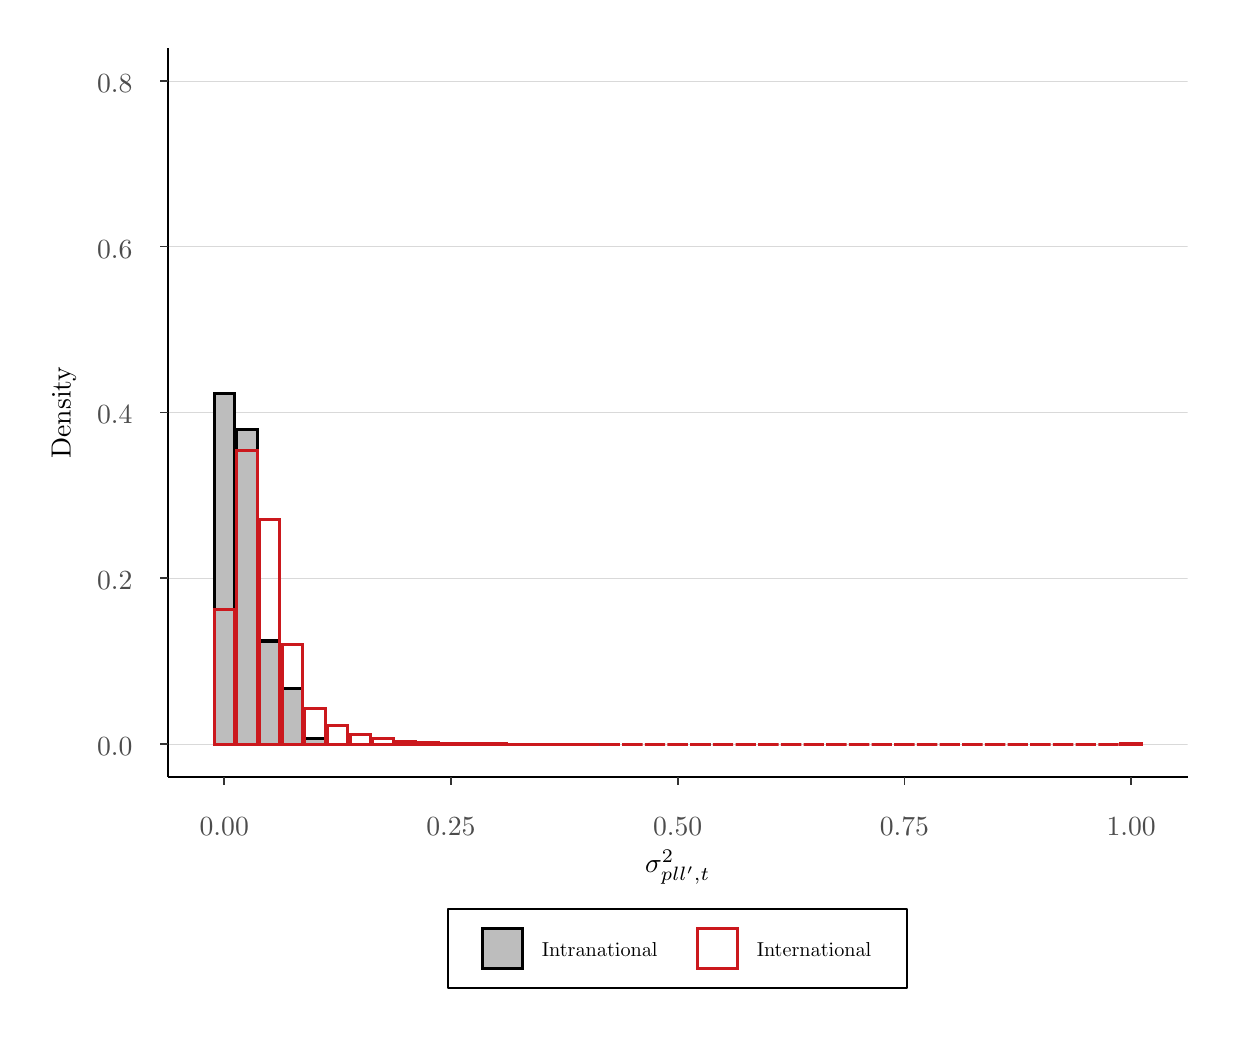
\begin{tikzpicture}[x=1pt,y=1pt]
\definecolor{fillColor}{RGB}{255,255,255}
\path[use as bounding box,fill=fillColor,fill opacity=0.00] (0,0) rectangle (433.62,361.35);
\begin{scope}
\path[clip] (  0.00,  0.00) rectangle (433.62,361.35);
\definecolor{drawColor}{RGB}{255,255,255}
\definecolor{fillColor}{RGB}{255,255,255}

\path[draw=drawColor,line width= 0.6pt,line join=round,line cap=round,fill=fillColor] (  0.00,  0.00) rectangle (433.62,361.35);
\end{scope}
\begin{scope}
\path[clip] ( 50.59, 90.50) rectangle (419.17,354.12);
\definecolor{drawColor}{RGB}{255,255,255}

\path[draw=drawColor,line width= 0.3pt,line join=round] ( 50.59,132.44) --
	(419.17,132.44);

\path[draw=drawColor,line width= 0.3pt,line join=round] ( 50.59,192.35) --
	(419.17,192.35);

\path[draw=drawColor,line width= 0.3pt,line join=round] ( 50.59,252.27) --
	(419.17,252.27);

\path[draw=drawColor,line width= 0.3pt,line join=round] ( 50.59,312.18) --
	(419.17,312.18);

\path[draw=drawColor,line width= 0.3pt,line join=round] (111.99, 90.50) --
	(111.99,354.12);

\path[draw=drawColor,line width= 0.3pt,line join=round] (193.92, 90.50) --
	(193.92,354.12);

\path[draw=drawColor,line width= 0.3pt,line join=round] (275.84, 90.50) --
	(275.84,354.12);

\path[draw=drawColor,line width= 0.3pt,line join=round] (357.76, 90.50) --
	(357.76,354.12);
\definecolor{drawColor}{gray}{0.85}

\path[draw=drawColor,line width= 0.1pt,line join=round] ( 50.59,102.48) --
	(419.17,102.48);

\path[draw=drawColor,line width= 0.1pt,line join=round] ( 50.59,162.40) --
	(419.17,162.40);

\path[draw=drawColor,line width= 0.1pt,line join=round] ( 50.59,222.31) --
	(419.17,222.31);

\path[draw=drawColor,line width= 0.1pt,line join=round] ( 50.59,282.23) --
	(419.17,282.23);

\path[draw=drawColor,line width= 0.1pt,line join=round] ( 50.59,342.14) --
	(419.17,342.14);
\definecolor{drawColor}{RGB}{0,0,0}
\definecolor{fillColor}{gray}{0.74}

\path[draw=drawColor,line width= 1.1pt,line cap=rect,fill=fillColor] ( 67.34,102.48) rectangle ( 74.72,229.25);
\definecolor{drawColor}{RGB}{203,24,29}

\path[draw=drawColor,line width= 1.1pt,line cap=rect] ( 67.34,102.48) rectangle ( 74.72,151.24);
\definecolor{drawColor}{RGB}{0,0,0}

\path[draw=drawColor,line width= 1.1pt,line cap=rect,fill=fillColor] ( 75.54,102.48) rectangle ( 82.91,216.25);
\definecolor{drawColor}{RGB}{203,24,29}

\path[draw=drawColor,line width= 1.1pt,line cap=rect] ( 75.54,102.48) rectangle ( 82.91,208.68);
\definecolor{drawColor}{RGB}{0,0,0}

\path[draw=drawColor,line width= 1.1pt,line cap=rect,fill=fillColor] ( 83.73,102.48) rectangle ( 91.10,139.73);
\definecolor{drawColor}{RGB}{203,24,29}

\path[draw=drawColor,line width= 1.1pt,line cap=rect] ( 83.73,102.48) rectangle ( 91.10,183.50);
\definecolor{drawColor}{RGB}{0,0,0}

\path[draw=drawColor,line width= 1.1pt,line cap=rect,fill=fillColor] ( 91.92,102.48) rectangle ( 99.29,122.41);
\definecolor{drawColor}{RGB}{203,24,29}

\path[draw=drawColor,line width= 1.1pt,line cap=rect] ( 91.92,102.48) rectangle ( 99.29,138.54);
\definecolor{drawColor}{RGB}{0,0,0}

\path[draw=drawColor,line width= 1.1pt,line cap=rect,fill=fillColor] (100.11,102.48) rectangle (107.49,104.33);
\definecolor{drawColor}{RGB}{203,24,29}

\path[draw=drawColor,line width= 1.1pt,line cap=rect] (100.11,102.48) rectangle (107.49,115.49);
\definecolor{drawColor}{RGB}{0,0,0}

\path[draw=drawColor,line width= 1.1pt,line cap=rect,fill=fillColor] (108.31,102.48) rectangle (115.68,102.49);
\definecolor{drawColor}{RGB}{203,24,29}

\path[draw=drawColor,line width= 1.1pt,line cap=rect] (108.31,102.48) rectangle (115.68,109.26);
\definecolor{drawColor}{RGB}{0,0,0}

\path[draw=drawColor,line width= 1.1pt,line cap=rect,fill=fillColor] (116.50,102.48) rectangle (123.87,102.48);
\definecolor{drawColor}{RGB}{203,24,29}

\path[draw=drawColor,line width= 1.1pt,line cap=rect] (116.50,102.48) rectangle (123.87,106.08);
\definecolor{drawColor}{RGB}{0,0,0}

\path[draw=drawColor,line width= 1.1pt,line cap=rect,fill=fillColor] (124.69,102.48) rectangle (132.06,102.48);
\definecolor{drawColor}{RGB}{203,24,29}

\path[draw=drawColor,line width= 1.1pt,line cap=rect] (124.69,102.48) rectangle (132.06,104.63);
\definecolor{drawColor}{RGB}{0,0,0}

\path[draw=drawColor,line width= 1.1pt,line cap=rect,fill=fillColor] (132.88,102.48) rectangle (140.26,102.48);
\definecolor{drawColor}{RGB}{203,24,29}

\path[draw=drawColor,line width= 1.1pt,line cap=rect] (132.88,102.48) rectangle (140.26,103.44);
\definecolor{drawColor}{RGB}{0,0,0}

\path[draw=drawColor,line width= 1.1pt,line cap=rect,fill=fillColor] (141.08,102.48) rectangle (148.45,102.48);
\definecolor{drawColor}{RGB}{203,24,29}

\path[draw=drawColor,line width= 1.1pt,line cap=rect] (141.08,102.48) rectangle (148.45,102.92);
\definecolor{drawColor}{RGB}{0,0,0}

\path[draw=drawColor,line width= 1.1pt,line cap=rect,fill=fillColor] (149.27,102.48) rectangle (156.64,102.48);
\definecolor{drawColor}{RGB}{203,24,29}

\path[draw=drawColor,line width= 1.1pt,line cap=rect] (149.27,102.48) rectangle (156.64,102.71);
\definecolor{drawColor}{RGB}{0,0,0}

\path[draw=drawColor,line width= 1.1pt,line cap=rect,fill=fillColor] (157.46,102.48) rectangle (164.83,102.48);
\definecolor{drawColor}{RGB}{203,24,29}

\path[draw=drawColor,line width= 1.1pt,line cap=rect] (157.46,102.48) rectangle (164.83,102.55);
\definecolor{drawColor}{RGB}{0,0,0}

\path[draw=drawColor,line width= 1.1pt,line cap=rect,fill=fillColor] (165.65,102.48) rectangle (173.03,102.48);
\definecolor{drawColor}{RGB}{203,24,29}

\path[draw=drawColor,line width= 1.1pt,line cap=rect] (165.65,102.48) rectangle (173.03,102.51);
\definecolor{drawColor}{RGB}{0,0,0}

\path[draw=drawColor,line width= 1.1pt,line cap=rect,fill=fillColor] (173.85,102.48) rectangle (181.22,102.48);
\definecolor{drawColor}{RGB}{203,24,29}

\path[draw=drawColor,line width= 1.1pt,line cap=rect] (173.85,102.48) rectangle (181.22,102.49);
\definecolor{drawColor}{RGB}{0,0,0}

\path[draw=drawColor,line width= 1.1pt,line cap=rect,fill=fillColor] (182.04,102.48) rectangle (189.41,102.48);
\definecolor{drawColor}{RGB}{203,24,29}

\path[draw=drawColor,line width= 1.1pt,line cap=rect] (182.04,102.48) rectangle (189.41,102.49);
\definecolor{drawColor}{RGB}{0,0,0}

\path[draw=drawColor,line width= 1.1pt,line cap=rect,fill=fillColor] (190.23,102.48) rectangle (197.60,102.48);
\definecolor{drawColor}{RGB}{203,24,29}

\path[draw=drawColor,line width= 1.1pt,line cap=rect] (190.23,102.48) rectangle (197.60,102.49);
\definecolor{drawColor}{RGB}{0,0,0}

\path[draw=drawColor,line width= 1.1pt,line cap=rect,fill=fillColor] (198.42,102.48) rectangle (205.80,102.48);
\definecolor{drawColor}{RGB}{203,24,29}

\path[draw=drawColor,line width= 1.1pt,line cap=rect] (198.42,102.48) rectangle (205.80,102.49);
\definecolor{drawColor}{RGB}{0,0,0}

\path[draw=drawColor,line width= 1.1pt,line cap=rect,fill=fillColor] (206.61,102.48) rectangle (213.99,102.48);
\definecolor{drawColor}{RGB}{203,24,29}

\path[draw=drawColor,line width= 1.1pt,line cap=rect] (206.61,102.48) rectangle (213.99,102.48);

\path[draw=drawColor,line width= 1.1pt,line cap=rect] (214.81,102.48) rectangle (222.18,102.48);

\path[draw=drawColor,line width= 1.1pt,line cap=rect] (223.00,102.48) rectangle (230.37,102.48);

\path[draw=drawColor,line width= 1.1pt,line cap=rect] (231.19,102.48) rectangle (238.56,102.48);
\definecolor{drawColor}{RGB}{0,0,0}

\path[draw=drawColor,line width= 1.1pt,line cap=rect,fill=fillColor] (239.38,102.48) rectangle (246.76,102.48);
\definecolor{drawColor}{RGB}{203,24,29}

\path[draw=drawColor,line width= 1.1pt,line cap=rect] (239.38,102.48) rectangle (246.76,102.48);

\path[draw=drawColor,line width= 1.1pt,line cap=rect] (247.58,102.48) rectangle (254.95,102.48);

\path[draw=drawColor,line width= 1.1pt,line cap=rect] (255.77,102.48) rectangle (263.14,102.48);

\path[draw=drawColor,line width= 1.1pt,line cap=rect] (263.96,102.48) rectangle (271.33,102.48);

\path[draw=drawColor,line width= 1.1pt,line cap=rect] (272.15,102.48) rectangle (279.53,102.48);

\path[draw=drawColor,line width= 1.1pt,line cap=rect] (280.35,102.48) rectangle (287.72,102.48);

\path[draw=drawColor,line width= 1.1pt,line cap=rect] (288.54,102.48) rectangle (295.91,102.48);

\path[draw=drawColor,line width= 1.1pt,line cap=rect] (296.73,102.48) rectangle (304.10,102.48);

\path[draw=drawColor,line width= 1.1pt,line cap=rect] (304.92,102.48) rectangle (312.30,102.48);

\path[draw=drawColor,line width= 1.1pt,line cap=rect] (313.12,102.48) rectangle (320.49,102.48);

\path[draw=drawColor,line width= 1.1pt,line cap=rect] (321.31,102.48) rectangle (328.68,102.48);

\path[draw=drawColor,line width= 1.1pt,line cap=rect] (329.50,102.48) rectangle (336.87,102.48);

\path[draw=drawColor,line width= 1.1pt,line cap=rect] (337.69,102.48) rectangle (345.07,102.48);

\path[draw=drawColor,line width= 1.1pt,line cap=rect] (345.89,102.48) rectangle (353.26,102.48);

\path[draw=drawColor,line width= 1.1pt,line cap=rect] (354.08,102.48) rectangle (361.45,102.48);

\path[draw=drawColor,line width= 1.1pt,line cap=rect] (362.27,102.48) rectangle (369.64,102.48);

\path[draw=drawColor,line width= 1.1pt,line cap=rect] (370.46,102.48) rectangle (377.84,102.48);

\path[draw=drawColor,line width= 1.1pt,line cap=rect] (378.65,102.48) rectangle (386.03,102.48);

\path[draw=drawColor,line width= 1.1pt,line cap=rect] (386.85,102.48) rectangle (394.22,102.48);
\definecolor{drawColor}{RGB}{0,0,0}

\path[draw=drawColor,line width= 1.1pt,line cap=rect,fill=fillColor] (395.04,102.48) rectangle (402.41,102.48);
\definecolor{drawColor}{RGB}{203,24,29}

\path[draw=drawColor,line width= 1.1pt,line cap=rect] (395.04,102.48) rectangle (402.41,102.73);
\end{scope}
\begin{scope}
\path[clip] (  0.00,  0.00) rectangle (433.62,361.35);
\definecolor{drawColor}{RGB}{0,0,0}

\path[draw=drawColor,line width= 0.6pt,line join=round] ( 50.59, 90.50) --
	( 50.59,354.12);
\end{scope}
\begin{scope}
\path[clip] (  0.00,  0.00) rectangle (433.62,361.35);
\definecolor{drawColor}{gray}{0.30}

\node[text=drawColor,anchor=base east,inner sep=0pt, outer sep=0pt, scale=  1.00] at ( 37.84, 98.35) {0.0};

\node[text=drawColor,anchor=base east,inner sep=0pt, outer sep=0pt, scale=  1.00] at ( 37.84,158.26) {0.2};

\node[text=drawColor,anchor=base east,inner sep=0pt, outer sep=0pt, scale=  1.00] at ( 37.84,218.18) {0.4};

\node[text=drawColor,anchor=base east,inner sep=0pt, outer sep=0pt, scale=  1.00] at ( 37.84,278.09) {0.6};

\node[text=drawColor,anchor=base east,inner sep=0pt, outer sep=0pt, scale=  1.00] at ( 37.84,338.01) {0.8};
\end{scope}
\begin{scope}
\path[clip] (  0.00,  0.00) rectangle (433.62,361.35);
\definecolor{drawColor}{gray}{0.20}

\path[draw=drawColor,line width= 0.6pt,line join=round] ( 47.84,102.48) --
	( 50.59,102.48);

\path[draw=drawColor,line width= 0.6pt,line join=round] ( 47.84,162.40) --
	( 50.59,162.40);

\path[draw=drawColor,line width= 0.6pt,line join=round] ( 47.84,222.31) --
	( 50.59,222.31);

\path[draw=drawColor,line width= 0.6pt,line join=round] ( 47.84,282.23) --
	( 50.59,282.23);

\path[draw=drawColor,line width= 0.6pt,line join=round] ( 47.84,342.14) --
	( 50.59,342.14);
\end{scope}
\begin{scope}
\path[clip] (  0.00,  0.00) rectangle (433.62,361.35);
\definecolor{drawColor}{RGB}{0,0,0}

\path[draw=drawColor,line width= 0.6pt,line join=round] ( 50.59, 90.50) --
	(419.17, 90.50);
\end{scope}
\begin{scope}
\path[clip] (  0.00,  0.00) rectangle (433.62,361.35);
\definecolor{drawColor}{gray}{0.20}

\path[draw=drawColor,line width= 0.6pt,line join=round] ( 71.03, 87.75) --
	( 71.03, 90.50);

\path[draw=drawColor,line width= 0.6pt,line join=round] (152.95, 87.75) --
	(152.95, 90.50);

\path[draw=drawColor,line width= 0.6pt,line join=round] (234.88, 87.75) --
	(234.88, 90.50);

\path[draw=drawColor,line width= 0.6pt,line join=round] (316.80, 87.75) --
	(316.80, 90.50);

\path[draw=drawColor,line width= 0.6pt,line join=round] (398.73, 87.75) --
	(398.73, 90.50);
\end{scope}
\begin{scope}
\path[clip] (  0.00,  0.00) rectangle (433.62,361.35);
\definecolor{drawColor}{gray}{0.30}

\node[text=drawColor,anchor=base,inner sep=0pt, outer sep=0pt, scale=  1.00] at ( 71.03, 69.48) {0.00};

\node[text=drawColor,anchor=base,inner sep=0pt, outer sep=0pt, scale=  1.00] at (152.95, 69.48) {0.25};

\node[text=drawColor,anchor=base,inner sep=0pt, outer sep=0pt, scale=  1.00] at (234.88, 69.48) {0.50};

\node[text=drawColor,anchor=base,inner sep=0pt, outer sep=0pt, scale=  1.00] at (316.80, 69.48) {0.75};

\node[text=drawColor,anchor=base,inner sep=0pt, outer sep=0pt, scale=  1.00] at (398.73, 69.48) {1.00};
\end{scope}
\begin{scope}
\path[clip] (  0.00,  0.00) rectangle (433.62,361.35);
\definecolor{drawColor}{RGB}{0,0,0}

\node[text=drawColor,anchor=base,inner sep=0pt, outer sep=0pt, scale=  1.00] at (234.88, 56.13) {$\sigma^{2}_{pll',t}$};
\end{scope}
\begin{scope}
\path[clip] (  0.00,  0.00) rectangle (433.62,361.35);
\definecolor{drawColor}{RGB}{0,0,0}

\node[text=drawColor,rotate= 90.00,anchor=base,inner sep=0pt, outer sep=0pt, scale=  1.00] at ( 15.49,222.31) {Density};
\end{scope}
\begin{scope}
\path[clip] (  0.00,  0.00) rectangle (433.62,361.35);
\definecolor{drawColor}{RGB}{0,0,0}
\definecolor{fillColor}{RGB}{255,255,255}

\path[draw=drawColor,line width= 0.6pt,line join=round,line cap=round,fill=fillColor] (151.97, 14.45) rectangle (317.79, 42.80);
\end{scope}
\begin{scope}
\path[clip] (  0.00,  0.00) rectangle (433.62,361.35);

\path[] (162.97, 19.95) rectangle (180.32, 37.30);
\end{scope}
\begin{scope}
\path[clip] (  0.00,  0.00) rectangle (433.62,361.35);
\definecolor{drawColor}{RGB}{0,0,0}
\definecolor{fillColor}{gray}{0.74}

\path[draw=drawColor,line width= 1.1pt,line cap=rect,fill=fillColor] (164.39, 21.38) rectangle (178.89, 35.88);
\end{scope}
\begin{scope}
\path[clip] (  0.00,  0.00) rectangle (433.62,361.35);

\path[] (240.62, 19.95) rectangle (257.96, 37.30);
\end{scope}
\begin{scope}
\path[clip] (  0.00,  0.00) rectangle (433.62,361.35);
\definecolor{drawColor}{RGB}{203,24,29}

\path[draw=drawColor,line width= 1.1pt,line cap=rect] (242.04, 21.38) rectangle (256.54, 35.88);
\end{scope}
\begin{scope}
\path[clip] (  0.00,  0.00) rectangle (433.62,361.35);
\definecolor{drawColor}{RGB}{0,0,0}

\node[text=drawColor,anchor=base west,inner sep=0pt, outer sep=0pt, scale=  0.73] at (185.82, 25.60) {Intranational};
\end{scope}
\begin{scope}
\path[clip] (  0.00,  0.00) rectangle (433.62,361.35);
\definecolor{drawColor}{RGB}{0,0,0}

\node[text=drawColor,anchor=base west,inner sep=0pt, outer sep=0pt, scale=  0.73] at (263.46, 25.60) {International};
\end{scope}
\end{tikzpicture}
}
     \end{subfigure}
     \parbox{\textwidth}{
        \begin{spacing}{1} 
            {\footnotesize 
            \textit{Notes}: This figure plots the distribution of the variance of log LOP deviations across product category-year-NUTS2-region pairs. The grey bars plot the conditional distribution for intranational pairs, and the red bars do the same for international pairs. We compute these distributions in three steps. First, we compute LOP deviations and winsorize the distribution symmetrically at 3 log points. Second, we compute the variance within product category-year-region pair cells. Finally, we bin the variance into 100 separate bins and compute for each bin the number of transactions, associated with the variances, that fall into each bin. Panel (a) replicates the result we show in the paper and is based on pooling across households and stores when computing price differences. Panel (b) computes price differences for identical product varieties within store types. Panel (c) computes price differences for identical product varieties within household types. Panel (d) computes price differences for identical product varieties within stores and household types.}
        \end{spacing}}
 \end{figure} 

 \begin{figure}[H]
    \centering
    \caption{Absolute LOP deviations: Years}
    \label{fig: app_redform_sd_years}
    % Created by tikzDevice version 0.12.3.1 on 2022-08-29 14:40:03
% !TEX encoding = UTF-8 Unicode
\begin{tikzpicture}[x=1pt,y=1pt]
\definecolor{fillColor}{RGB}{255,255,255}
\path[use as bounding box,fill=fillColor,fill opacity=0.00] (0,0) rectangle (433.62,361.35);
\begin{scope}
\path[clip] (  0.00,  0.00) rectangle (433.62,361.35);
\definecolor{drawColor}{RGB}{255,255,255}
\definecolor{fillColor}{RGB}{255,255,255}

\path[draw=drawColor,line width= 0.6pt,line join=round,line cap=round,fill=fillColor] ( -0.00,  0.00) rectangle (433.62,361.35);
\end{scope}
\begin{scope}
\path[clip] ( 50.19, 51.15) rectangle (419.17,354.12);
\definecolor{drawColor}{RGB}{255,255,255}

\path[draw=drawColor,line width= 0.3pt,line join=round] ( 50.19,110.83) --
	(419.17,110.83);

\path[draw=drawColor,line width= 0.3pt,line join=round] ( 50.19,202.64) --
	(419.17,202.64);

\path[draw=drawColor,line width= 0.3pt,line join=round] ( 50.19,294.45) --
	(419.17,294.45);
\definecolor{drawColor}{gray}{0.85}

\path[draw=drawColor,line width= 0.1pt,line join=round] ( 50.19, 64.92) --
	(419.17, 64.92);

\path[draw=drawColor,line width= 0.1pt,line join=round] ( 50.19,156.73) --
	(419.17,156.73);

\path[draw=drawColor,line width= 0.1pt,line join=round] ( 50.19,248.54) --
	(419.17,248.54);

\path[draw=drawColor,line width= 0.1pt,line join=round] ( 50.19,340.35) --
	(419.17,340.35);
\definecolor{drawColor}{RGB}{0,0,0}

\path[draw=drawColor,line width= 0.4pt,line join=round,line cap=round] (397.46,173.98) circle (  2.50);

\path[draw=drawColor,line width= 0.4pt,line join=round,line cap=round] (361.29,177.54) circle (  2.50);

\path[draw=drawColor,line width= 0.4pt,line join=round,line cap=round] (325.11,177.84) circle (  2.50);

\path[draw=drawColor,line width= 0.4pt,line join=round,line cap=round] (288.94,181.16) circle (  2.50);

\path[draw=drawColor,line width= 0.4pt,line join=round,line cap=round] (252.77,180.93) circle (  2.50);

\path[draw=drawColor,line width= 0.4pt,line join=round,line cap=round] (216.59,180.22) circle (  2.50);

\path[draw=drawColor,line width= 0.4pt,line join=round,line cap=round] (180.42,176.33) circle (  2.50);

\path[draw=drawColor,line width= 0.4pt,line join=round,line cap=round] (144.25,178.32) circle (  2.50);

\path[draw=drawColor,line width= 0.4pt,line join=round,line cap=round] (108.07,182.17) circle (  2.50);

\path[draw=drawColor,line width= 0.4pt,line join=round,line cap=round] ( 71.90,181.72) circle (  2.50);
\definecolor{drawColor}{RGB}{203,24,29}

\path[draw=drawColor,line width= 0.4pt,line join=round,line cap=round] (393.93,211.49) --
	(397.46,215.02) --
	(400.99,211.49) --
	(397.46,207.96) --
	cycle;

\path[draw=drawColor,line width= 0.4pt,line join=round,line cap=round] (357.76,199.22) --
	(361.29,202.75) --
	(364.82,199.22) --
	(361.29,195.68) --
	cycle;

\path[draw=drawColor,line width= 0.4pt,line join=round,line cap=round] (321.58,204.28) --
	(325.11,207.81) --
	(328.65,204.28) --
	(325.11,200.75) --
	cycle;

\path[draw=drawColor,line width= 0.4pt,line join=round,line cap=round] (285.41,201.02) --
	(288.94,204.55) --
	(292.47,201.02) --
	(288.94,197.49) --
	cycle;

\path[draw=drawColor,line width= 0.4pt,line join=round,line cap=round] (249.23,202.06) --
	(252.77,205.59) --
	(256.30,202.06) --
	(252.77,198.53) --
	cycle;

\path[draw=drawColor,line width= 0.4pt,line join=round,line cap=round] (213.06,202.50) --
	(216.59,206.04) --
	(220.13,202.50) --
	(216.59,198.97) --
	cycle;

\path[draw=drawColor,line width= 0.4pt,line join=round,line cap=round] (176.89,204.32) --
	(180.42,207.85) --
	(183.95,204.32) --
	(180.42,200.79) --
	cycle;

\path[draw=drawColor,line width= 0.4pt,line join=round,line cap=round] (140.71,207.20) --
	(144.25,210.73) --
	(147.78,207.20) --
	(144.25,203.66) --
	cycle;

\path[draw=drawColor,line width= 0.4pt,line join=round,line cap=round] (104.54,209.48) --
	(108.07,213.02) --
	(111.60,209.48) --
	(108.07,205.95) --
	cycle;

\path[draw=drawColor,line width= 0.4pt,line join=round,line cap=round] ( 68.37,219.28) --
	( 71.90,222.82) --
	( 75.43,219.28) --
	( 71.90,215.75) --
	cycle;
\definecolor{drawColor}{RGB}{0,0,0}

\path[draw=drawColor,draw opacity=0.75,line width= 0.6pt,line join=round] (393.84,214.64) --
	(401.08,214.64);

\path[draw=drawColor,draw opacity=0.75,line width= 0.6pt,line join=round] (397.46,214.64) --
	(397.46,208.34);

\path[draw=drawColor,draw opacity=0.75,line width= 0.6pt,line join=round] (393.84,208.34) --
	(401.08,208.34);

\path[draw=drawColor,draw opacity=0.75,line width= 0.6pt,line join=round] (357.67,201.22) --
	(364.91,201.22);

\path[draw=drawColor,draw opacity=0.75,line width= 0.6pt,line join=round] (361.29,201.22) --
	(361.29,197.21);

\path[draw=drawColor,draw opacity=0.75,line width= 0.6pt,line join=round] (357.67,197.21) --
	(364.91,197.21);

\path[draw=drawColor,draw opacity=0.75,line width= 0.6pt,line join=round] (321.50,206.27) --
	(328.73,206.27);

\path[draw=drawColor,draw opacity=0.75,line width= 0.6pt,line join=round] (325.11,206.27) --
	(325.11,202.29);

\path[draw=drawColor,draw opacity=0.75,line width= 0.6pt,line join=round] (321.50,202.29) --
	(328.73,202.29);

\path[draw=drawColor,draw opacity=0.75,line width= 0.6pt,line join=round] (285.32,202.94) --
	(292.56,202.94);

\path[draw=drawColor,draw opacity=0.75,line width= 0.6pt,line join=round] (288.94,202.94) --
	(288.94,199.09);

\path[draw=drawColor,draw opacity=0.75,line width= 0.6pt,line join=round] (285.32,199.09) --
	(292.56,199.09);

\path[draw=drawColor,draw opacity=0.75,line width= 0.6pt,line join=round] (249.15,204.76) --
	(256.38,204.76);

\path[draw=drawColor,draw opacity=0.75,line width= 0.6pt,line join=round] (252.77,204.76) --
	(252.77,199.36);

\path[draw=drawColor,draw opacity=0.75,line width= 0.6pt,line join=round] (249.15,199.36) --
	(256.38,199.36);

\path[draw=drawColor,draw opacity=0.75,line width= 0.6pt,line join=round] (212.98,204.75) --
	(220.21,204.75);

\path[draw=drawColor,draw opacity=0.75,line width= 0.6pt,line join=round] (216.59,204.75) --
	(216.59,200.26);

\path[draw=drawColor,draw opacity=0.75,line width= 0.6pt,line join=round] (212.98,200.26) --
	(220.21,200.26);

\path[draw=drawColor,draw opacity=0.75,line width= 0.6pt,line join=round] (176.80,207.01) --
	(184.04,207.01);

\path[draw=drawColor,draw opacity=0.75,line width= 0.6pt,line join=round] (180.42,207.01) --
	(180.42,201.63);

\path[draw=drawColor,draw opacity=0.75,line width= 0.6pt,line join=round] (176.80,201.63) --
	(184.04,201.63);

\path[draw=drawColor,draw opacity=0.75,line width= 0.6pt,line join=round] (140.63,209.65) --
	(147.86,209.65);

\path[draw=drawColor,draw opacity=0.75,line width= 0.6pt,line join=round] (144.25,209.65) --
	(144.25,204.74);

\path[draw=drawColor,draw opacity=0.75,line width= 0.6pt,line join=round] (140.63,204.74) --
	(147.86,204.74);

\path[draw=drawColor,draw opacity=0.75,line width= 0.6pt,line join=round] (104.45,212.52) --
	(111.69,212.52);

\path[draw=drawColor,draw opacity=0.75,line width= 0.6pt,line join=round] (108.07,212.52) --
	(108.07,206.45);

\path[draw=drawColor,draw opacity=0.75,line width= 0.6pt,line join=round] (104.45,206.45) --
	(111.69,206.45);

\path[draw=drawColor,draw opacity=0.75,line width= 0.6pt,line join=round] ( 68.28,222.06) --
	( 75.52,222.06);

\path[draw=drawColor,draw opacity=0.75,line width= 0.6pt,line join=round] ( 71.90,222.06) --
	( 71.90,216.51);

\path[draw=drawColor,draw opacity=0.75,line width= 0.6pt,line join=round] ( 68.28,216.51) --
	( 75.52,216.51);
\end{scope}
\begin{scope}
\path[clip] (  0.00,  0.00) rectangle (433.62,361.35);
\definecolor{drawColor}{RGB}{0,0,0}

\path[draw=drawColor,line width= 0.6pt,line join=round] ( 50.19, 51.15) --
	( 50.19,354.12);
\end{scope}
\begin{scope}
\path[clip] (  0.00,  0.00) rectangle (433.62,361.35);
\definecolor{drawColor}{gray}{0.30}

\node[text=drawColor,anchor=base east,inner sep=0pt, outer sep=0pt, scale=  1.00] at ( 37.44, 60.79) {0.0};

\node[text=drawColor,anchor=base east,inner sep=0pt, outer sep=0pt, scale=  1.00] at ( 37.44,152.60) {0.1};

\node[text=drawColor,anchor=base east,inner sep=0pt, outer sep=0pt, scale=  1.00] at ( 37.44,244.41) {0.2};

\node[text=drawColor,anchor=base east,inner sep=0pt, outer sep=0pt, scale=  1.00] at ( 37.44,336.22) {0.3};
\end{scope}
\begin{scope}
\path[clip] (  0.00,  0.00) rectangle (433.62,361.35);
\definecolor{drawColor}{gray}{0.20}

\path[draw=drawColor,line width= 0.6pt,line join=round] ( 47.44, 64.92) --
	( 50.19, 64.92);

\path[draw=drawColor,line width= 0.6pt,line join=round] ( 47.44,156.73) --
	( 50.19,156.73);

\path[draw=drawColor,line width= 0.6pt,line join=round] ( 47.44,248.54) --
	( 50.19,248.54);

\path[draw=drawColor,line width= 0.6pt,line join=round] ( 47.44,340.35) --
	( 50.19,340.35);
\end{scope}
\begin{scope}
\path[clip] (  0.00,  0.00) rectangle (433.62,361.35);
\definecolor{drawColor}{RGB}{0,0,0}

\path[draw=drawColor,line width= 0.6pt,line join=round] ( 50.19, 51.15) --
	(419.17, 51.15);
\end{scope}
\begin{scope}
\path[clip] (  0.00,  0.00) rectangle (433.62,361.35);
\definecolor{drawColor}{gray}{0.20}

\path[draw=drawColor,line width= 0.6pt,line join=round] ( 71.90, 48.40) --
	( 71.90, 51.15);

\path[draw=drawColor,line width= 0.6pt,line join=round] (108.07, 48.40) --
	(108.07, 51.15);

\path[draw=drawColor,line width= 0.6pt,line join=round] (144.25, 48.40) --
	(144.25, 51.15);

\path[draw=drawColor,line width= 0.6pt,line join=round] (180.42, 48.40) --
	(180.42, 51.15);

\path[draw=drawColor,line width= 0.6pt,line join=round] (216.59, 48.40) --
	(216.59, 51.15);

\path[draw=drawColor,line width= 0.6pt,line join=round] (252.77, 48.40) --
	(252.77, 51.15);

\path[draw=drawColor,line width= 0.6pt,line join=round] (288.94, 48.40) --
	(288.94, 51.15);

\path[draw=drawColor,line width= 0.6pt,line join=round] (325.11, 48.40) --
	(325.11, 51.15);

\path[draw=drawColor,line width= 0.6pt,line join=round] (361.29, 48.40) --
	(361.29, 51.15);

\path[draw=drawColor,line width= 0.6pt,line join=round] (397.46, 48.40) --
	(397.46, 51.15);
\end{scope}
\begin{scope}
\path[clip] (  0.00,  0.00) rectangle (433.62,361.35);
\definecolor{drawColor}{gray}{0.30}

\node[text=drawColor,anchor=base,inner sep=0pt, outer sep=0pt, scale=  1.00] at ( 71.90, 30.14) {2010};

\node[text=drawColor,anchor=base,inner sep=0pt, outer sep=0pt, scale=  1.00] at (108.07, 30.14) {2011};

\node[text=drawColor,anchor=base,inner sep=0pt, outer sep=0pt, scale=  1.00] at (144.25, 30.14) {2012};

\node[text=drawColor,anchor=base,inner sep=0pt, outer sep=0pt, scale=  1.00] at (180.42, 30.14) {2013};

\node[text=drawColor,anchor=base,inner sep=0pt, outer sep=0pt, scale=  1.00] at (216.59, 30.14) {2014};

\node[text=drawColor,anchor=base,inner sep=0pt, outer sep=0pt, scale=  1.00] at (252.77, 30.14) {2015};

\node[text=drawColor,anchor=base,inner sep=0pt, outer sep=0pt, scale=  1.00] at (288.94, 30.14) {2016};

\node[text=drawColor,anchor=base,inner sep=0pt, outer sep=0pt, scale=  1.00] at (325.11, 30.14) {2017};

\node[text=drawColor,anchor=base,inner sep=0pt, outer sep=0pt, scale=  1.00] at (361.29, 30.14) {2018};

\node[text=drawColor,anchor=base,inner sep=0pt, outer sep=0pt, scale=  1.00] at (397.46, 30.14) {2019};
\end{scope}
\begin{scope}
\path[clip] (  0.00,  0.00) rectangle (433.62,361.35);
\definecolor{drawColor}{RGB}{0,0,0}

\node[text=drawColor,anchor=base,inner sep=0pt, outer sep=0pt, scale=  1.00] at (234.68, 16.79) {Year};
\end{scope}
\begin{scope}
\path[clip] (  0.00,  0.00) rectangle (433.62,361.35);
\definecolor{drawColor}{RGB}{0,0,0}

\node[text=drawColor,anchor=base,inner sep=0pt, outer sep=0pt, scale=  1.00] at ( 12.33,198.51) {$\beta_{t}$};
\end{scope}
\end{tikzpicture}

     \parbox{\textwidth}{
        \begin{spacing}{1} 
            {\footnotesize 
            \textit{Notes}: This figure shows the results from estimating the following regression:
            $$ \sigma^{P,ll'}_{p,t} = \beta_t B_{ll'} + \gamma d_{ll'} + \theta_l + \theta_{l'} +\lambda_{p} + \varepsilon_{pll',t}$$ 
            The red diamonds are the $\beta_{t}$ coefficients and the error bars show 95\%-confidence intervals based on two-way clustered standard errors both at $l$-NUTS2 and at the $l^{'}$-NUTS2 level. The black circles show the average absolute price percentage price difference for region pairs within the same country.}
        \end{spacing}}
 \end{figure} 

 \begin{figure}[H]
    \centering
    \caption{Absolute LOP deviations: Categories}
    \label{fig: app_redform_sd_cats}
    % Created by tikzDevice version 0.12.3.1 on 2022-08-29 14:39:49
% !TEX encoding = UTF-8 Unicode
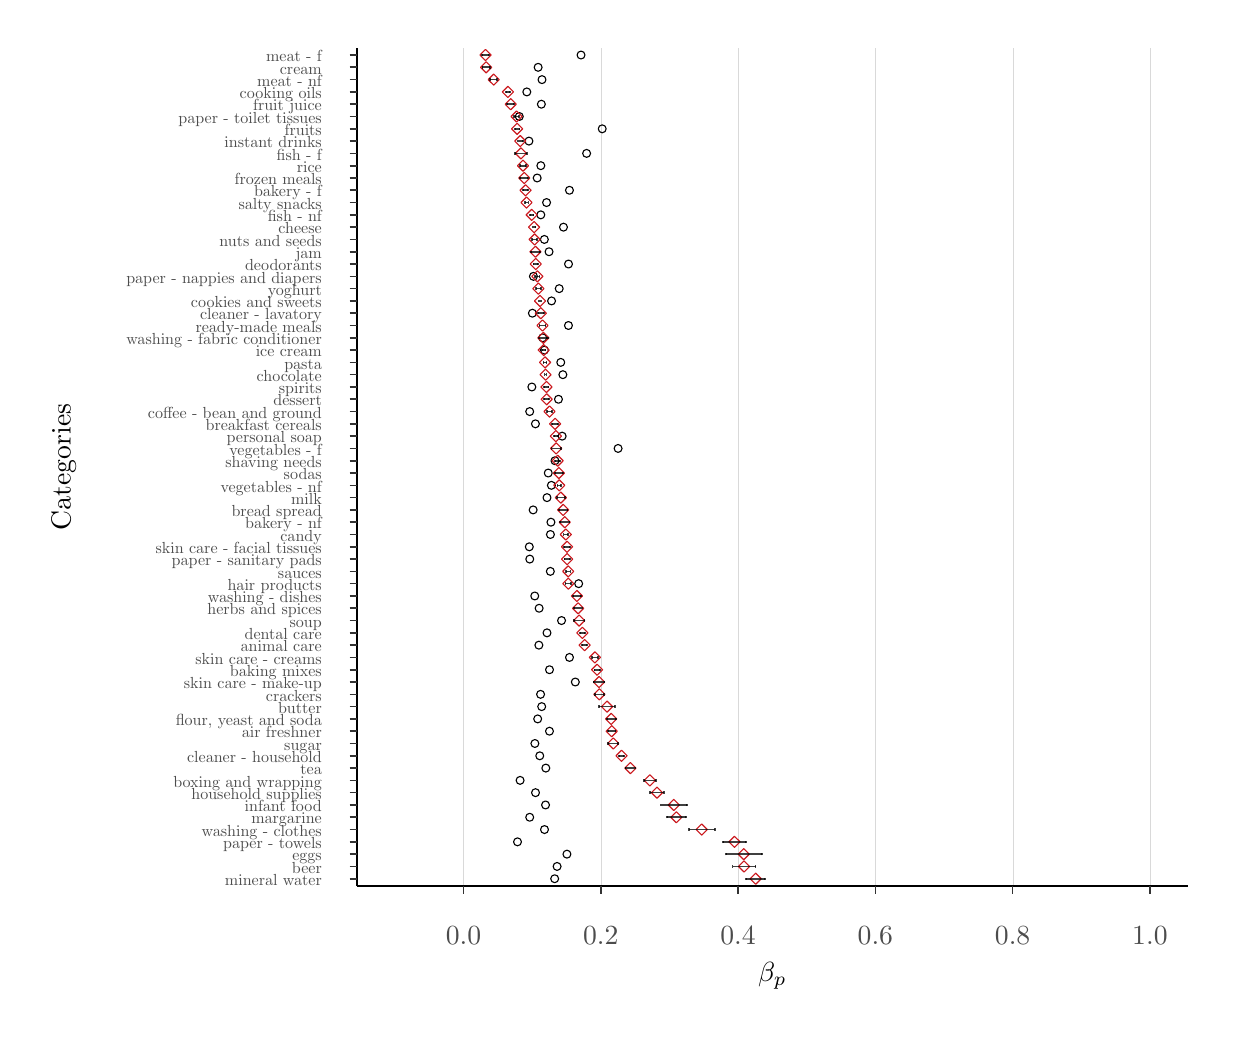
\begin{tikzpicture}[x=1pt,y=1pt]
\definecolor{fillColor}{RGB}{255,255,255}
\path[use as bounding box,fill=fillColor,fill opacity=0.00] (0,0) rectangle (433.62,361.35);
\begin{scope}
\path[clip] (  0.00,  0.00) rectangle (433.62,361.35);
\definecolor{drawColor}{RGB}{255,255,255}
\definecolor{fillColor}{RGB}{255,255,255}

\path[draw=drawColor,line width= 0.6pt,line join=round,line cap=round,fill=fillColor] (  0.00,  0.00) rectangle (433.62,361.35);
\end{scope}
\begin{scope}
\path[clip] (119.04, 51.15) rectangle (419.17,354.12);
\definecolor{drawColor}{RGB}{255,255,255}

\path[draw=drawColor,line width= 0.3pt,line join=round] (132.68, 51.15) --
	(132.68,354.12);

\path[draw=drawColor,line width= 0.3pt,line join=round] (182.29, 51.15) --
	(182.29,354.12);

\path[draw=drawColor,line width= 0.3pt,line join=round] (231.90, 51.15) --
	(231.90,354.12);

\path[draw=drawColor,line width= 0.3pt,line join=round] (281.51, 51.15) --
	(281.51,354.12);

\path[draw=drawColor,line width= 0.3pt,line join=round] (331.11, 51.15) --
	(331.11,354.12);

\path[draw=drawColor,line width= 0.3pt,line join=round] (380.72, 51.15) --
	(380.72,354.12);
\definecolor{drawColor}{gray}{0.85}

\path[draw=drawColor,line width= 0.1pt,line join=round] (157.49, 51.15) --
	(157.49,354.12);

\path[draw=drawColor,line width= 0.1pt,line join=round] (207.09, 51.15) --
	(207.09,354.12);

\path[draw=drawColor,line width= 0.1pt,line join=round] (256.70, 51.15) --
	(256.70,354.12);

\path[draw=drawColor,line width= 0.1pt,line join=round] (306.31, 51.15) --
	(306.31,354.12);

\path[draw=drawColor,line width= 0.1pt,line join=round] (355.92, 51.15) --
	(355.92,354.12);

\path[draw=drawColor,line width= 0.1pt,line join=round] (405.52, 51.15) --
	(405.52,354.12);
\definecolor{drawColor}{RGB}{0,0,0}

\path[draw=drawColor,line width= 0.4pt,line join=round,line cap=round] (192.07,267.05) circle (  1.43);

\path[draw=drawColor,line width= 0.4pt,line join=round,line cap=round] (186.11,249.28) circle (  1.43);

\path[draw=drawColor,line width= 0.4pt,line join=round,line cap=round] (183.23,155.99) circle (  1.43);

\path[draw=drawColor,line width= 0.4pt,line join=round,line cap=round] (186.75, 71.59) circle (  1.43);

\path[draw=drawColor,line width= 0.4pt,line join=round,line cap=round] (189.24,195.97) circle (  1.43);

\path[draw=drawColor,line width= 0.4pt,line join=round,line cap=round] (213.34,209.30) circle (  1.43);

\path[draw=drawColor,line width= 0.4pt,line join=round,line cap=round] (187.23, 93.80) circle (  1.43);

\path[draw=drawColor,line width= 0.4pt,line join=round,line cap=round] (183.28,102.69) circle (  1.43);

\path[draw=drawColor,line width= 0.4pt,line join=round,line cap=round] (182.18,231.51) circle (  1.43);

\path[draw=drawColor,line width= 0.4pt,line join=round,line cap=round] (192.91,147.11) circle (  1.43);

\path[draw=drawColor,line width= 0.4pt,line join=round,line cap=round] (188.11,200.42) circle (  1.43);

\path[draw=drawColor,line width= 0.4pt,line join=round,line cap=round] (197.89,124.90) circle (  1.43);

\path[draw=drawColor,line width= 0.4pt,line join=round,line cap=round] (181.26,173.76) circle (  1.43);

\path[draw=drawColor,line width= 0.4pt,line join=round,line cap=round] (195.78,133.78) circle (  1.43);

\path[draw=drawColor,line width= 0.4pt,line join=round,line cap=round] (190.54,204.86) circle (  1.43);

\path[draw=drawColor,line width= 0.4pt,line join=round,line cap=round] (188.86,164.88) circle (  1.43);

\path[draw=drawColor,line width= 0.4pt,line join=round,line cap=round] (187.50,298.15) circle (  1.43);

\path[draw=drawColor,line width= 0.4pt,line join=round,line cap=round] (185.43,311.48) circle (  1.43);

\path[draw=drawColor,line width= 0.4pt,line join=round,line cap=round] (195.41,253.73) circle (  1.43);

\path[draw=drawColor,line width= 0.4pt,line join=round,line cap=round] (193.13,213.74) circle (  1.43);

\path[draw=drawColor,line width= 0.4pt,line join=round,line cap=round] (192.63,240.40) circle (  1.43);

\path[draw=drawColor,line width= 0.4pt,line join=round,line cap=round] (177.00, 67.15) circle (  1.43);

\path[draw=drawColor,line width= 0.4pt,line join=round,line cap=round] (177.64,329.25) circle (  1.43);

\path[draw=drawColor,line width= 0.4pt,line join=round,line cap=round] (181.43,169.32) circle (  1.43);

\path[draw=drawColor,line width= 0.4pt,line join=round,line cap=round] (182.75,271.49) circle (  1.43);

\path[draw=drawColor,line width= 0.4pt,line join=round,line cap=round] (186.70,284.82) circle (  1.43);

\path[draw=drawColor,line width= 0.4pt,line join=round,line cap=round] (190.43, 53.82) circle (  1.43);

\path[draw=drawColor,line width= 0.4pt,line join=round,line cap=round] (187.65,191.53) circle (  1.43);

\path[draw=drawColor,line width= 0.4pt,line join=round,line cap=round] (185.85,342.57) circle (  1.43);

\path[draw=drawColor,line width= 0.4pt,line join=round,line cap=round] (199.95,351.46) circle (  1.43);

\path[draw=drawColor,line width= 0.4pt,line join=round,line cap=round] (181.41, 76.03) circle (  1.43);

\path[draw=drawColor,line width= 0.4pt,line join=round,line cap=round] (188.39,280.38) circle (  1.43);

\path[draw=drawColor,line width= 0.4pt,line join=round,line cap=round] (181.13,320.36) circle (  1.43);

\path[draw=drawColor,line width= 0.4pt,line join=round,line cap=round] (187.13, 80.47) circle (  1.43);

\path[draw=drawColor,line width= 0.4pt,line join=round,line cap=round] (186.73,244.84) circle (  1.43);

\path[draw=drawColor,line width= 0.4pt,line join=round,line cap=round] (183.51, 84.92) circle (  1.43);

\path[draw=drawColor,line width= 0.4pt,line join=round,line cap=round] (184.81,151.55) circle (  1.43);

\path[draw=drawColor,line width= 0.4pt,line join=round,line cap=round] (199.10,160.44) circle (  1.43);

\path[draw=drawColor,line width= 0.4pt,line join=round,line cap=round] (207.61,324.80) circle (  1.43);

\path[draw=drawColor,line width= 0.4pt,line join=round,line cap=round] (185.62,333.69) circle (  1.43);

\path[draw=drawColor,line width= 0.4pt,line join=round,line cap=round] (184.11,307.03) circle (  1.43);

\path[draw=drawColor,line width= 0.4pt,line join=round,line cap=round] (184.29,111.57) circle (  1.43);

\path[draw=drawColor,line width= 0.4pt,line join=round,line cap=round] (185.42,293.71) circle (  1.43);

\path[draw=drawColor,line width= 0.4pt,line join=round,line cap=round] (201.97,315.92) circle (  1.43);

\path[draw=drawColor,line width= 0.4pt,line join=round,line cap=round] (194.86, 62.70) circle (  1.43);

\path[draw=drawColor,line width= 0.4pt,line join=round,line cap=round] (191.80,227.07) circle (  1.43);

\path[draw=drawColor,line width= 0.4pt,line join=round,line cap=round] (195.43,275.94) circle (  1.43);

\path[draw=drawColor,line width= 0.4pt,line join=round,line cap=round] (187.65,142.67) circle (  1.43);

\path[draw=drawColor,line width= 0.4pt,line join=round,line cap=round] (184.45,347.02) circle (  1.43);

\path[draw=drawColor,line width= 0.4pt,line join=round,line cap=round] (185.33,120.45) circle (  1.43);

\path[draw=drawColor,line width= 0.4pt,line join=round,line cap=round] (180.36,338.13) circle (  1.43);

\path[draw=drawColor,line width= 0.4pt,line join=round,line cap=round] (189.30,262.61) circle (  1.43);

\path[draw=drawColor,line width= 0.4pt,line join=round,line cap=round] (181.41,222.63) circle (  1.43);

\path[draw=drawColor,line width= 0.4pt,line join=round,line cap=round] (182.38,258.17) circle (  1.43);

\path[draw=drawColor,line width= 0.4pt,line join=round,line cap=round] (185.04, 98.24) circle (  1.43);

\path[draw=drawColor,line width= 0.4pt,line join=round,line cap=round] (193.39,235.96) circle (  1.43);

\path[draw=drawColor,line width= 0.4pt,line join=round,line cap=round] (193.61,289.26) circle (  1.43);

\path[draw=drawColor,line width= 0.4pt,line join=round,line cap=round] (188.89,178.21) circle (  1.43);

\path[draw=drawColor,line width= 0.4pt,line join=round,line cap=round] (185.74,116.01) circle (  1.43);

\path[draw=drawColor,line width= 0.4pt,line join=round,line cap=round] (183.48,218.19) circle (  1.43);

\path[draw=drawColor,line width= 0.4pt,line join=round,line cap=round] (182.65,187.09) circle (  1.43);

\path[draw=drawColor,line width= 0.4pt,line join=round,line cap=round] (177.93, 89.36) circle (  1.43);

\path[draw=drawColor,line width= 0.4pt,line join=round,line cap=round] (191.30, 58.26) circle (  1.43);

\path[draw=drawColor,line width= 0.4pt,line join=round,line cap=round] (188.56,129.34) circle (  1.43);

\path[draw=drawColor,line width= 0.4pt,line join=round,line cap=round] (189.08,182.65) circle (  1.43);

\path[draw=drawColor,line width= 0.4pt,line join=round,line cap=round] (195.77,302.59) circle (  1.43);

\path[draw=drawColor,line width= 0.4pt,line join=round,line cap=round] (184.72,138.22) circle (  1.43);

\path[draw=drawColor,line width= 0.4pt,line join=round,line cap=round] (188.55,107.13) circle (  1.43);
\definecolor{drawColor}{RGB}{203,24,29}

\path[draw=drawColor,line width= 0.4pt,line join=round,line cap=round] (182.53,267.05) --
	(184.54,269.07) --
	(186.56,267.05) --
	(184.54,265.04) --
	cycle;

\path[draw=drawColor,line width= 0.4pt,line join=round,line cap=round] (184.33,249.28) --
	(186.35,251.30) --
	(188.37,249.28) --
	(186.35,247.27) --
	cycle;

\path[draw=drawColor,line width= 0.4pt,line join=round,line cap=round] (196.44,155.99) --
	(198.46,158.01) --
	(200.48,155.99) --
	(198.46,153.98) --
	cycle;

\path[draw=drawColor,line width= 0.4pt,line join=round,line cap=round] (241.55, 71.59) --
	(243.57, 73.61) --
	(245.59, 71.59) --
	(243.57, 69.57) --
	cycle;

\path[draw=drawColor,line width= 0.4pt,line join=round,line cap=round] (190.06,195.97) --
	(192.08,197.99) --
	(194.09,195.97) --
	(192.08,193.96) --
	cycle;

\path[draw=drawColor,line width= 0.4pt,line join=round,line cap=round] (188.95,209.30) --
	(190.97,211.32) --
	(192.99,209.30) --
	(190.97,207.28) --
	cycle;

\path[draw=drawColor,line width= 0.4pt,line join=round,line cap=round] (215.77, 93.80) --
	(217.79, 95.82) --
	(219.80, 93.80) --
	(217.79, 91.78) --
	cycle;

\path[draw=drawColor,line width= 0.4pt,line join=round,line cap=round] (209.59,102.69) --
	(211.61,104.70) --
	(213.62,102.69) --
	(211.61,100.67) --
	cycle;

\path[draw=drawColor,line width= 0.4pt,line join=round,line cap=round] (185.43,231.51) --
	(187.45,233.53) --
	(189.47,231.51) --
	(187.45,229.50) --
	cycle;

\path[draw=drawColor,line width= 0.4pt,line join=round,line cap=round] (197.25,147.11) --
	(199.27,149.13) --
	(201.28,147.11) --
	(199.27,145.09) --
	cycle;

\path[draw=drawColor,line width= 0.4pt,line join=round,line cap=round] (189.92,200.42) --
	(191.94,202.43) --
	(193.96,200.42) --
	(191.94,198.40) --
	cycle;

\path[draw=drawColor,line width= 0.4pt,line join=round,line cap=round] (204.44,124.90) --
	(206.46,126.91) --
	(208.48,124.90) --
	(206.46,122.88) --
	cycle;

\path[draw=drawColor,line width= 0.4pt,line join=round,line cap=round] (192.87,173.76) --
	(194.89,175.78) --
	(196.91,173.76) --
	(194.89,171.75) --
	cycle;

\path[draw=drawColor,line width= 0.4pt,line join=round,line cap=round] (202.95,133.78) --
	(204.96,135.80) --
	(206.98,133.78) --
	(204.96,131.76) --
	cycle;

\path[draw=drawColor,line width= 0.4pt,line join=round,line cap=round] (189.49,204.86) --
	(191.51,206.88) --
	(193.52,204.86) --
	(191.51,202.84) --
	cycle;

\path[draw=drawColor,line width= 0.4pt,line join=round,line cap=round] (193.31,164.88) --
	(195.33,166.90) --
	(197.34,164.88) --
	(195.33,162.86) --
	cycle;

\path[draw=drawColor,line width= 0.4pt,line join=round,line cap=round] (178.24,298.15) --
	(180.26,300.17) --
	(182.27,298.15) --
	(180.26,296.13) --
	cycle;

\path[draw=drawColor,line width= 0.4pt,line join=round,line cap=round] (176.97,311.48) --
	(178.99,313.49) --
	(181.00,311.48) --
	(178.99,309.46) --
	cycle;

\path[draw=drawColor,line width= 0.4pt,line join=round,line cap=round] (184.02,253.73) --
	(186.03,255.74) --
	(188.05,253.73) --
	(186.03,251.71) --
	cycle;

\path[draw=drawColor,line width= 0.4pt,line join=round,line cap=round] (188.85,213.74) --
	(190.87,215.76) --
	(192.88,213.74) --
	(190.87,211.73) --
	cycle;

\path[draw=drawColor,line width= 0.4pt,line join=round,line cap=round] (184.93,240.40) --
	(186.94,242.42) --
	(188.96,240.40) --
	(186.94,238.38) --
	cycle;

\path[draw=drawColor,line width= 0.4pt,line join=round,line cap=round] (253.38, 67.15) --
	(255.40, 69.16) --
	(257.42, 67.15) --
	(255.40, 65.13) --
	cycle;

\path[draw=drawColor,line width= 0.4pt,line join=round,line cap=round] (174.65,329.25) --
	(176.67,331.26) --
	(178.68,329.25) --
	(176.67,327.23) --
	cycle;

\path[draw=drawColor,line width= 0.4pt,line join=round,line cap=round] (192.90,169.32) --
	(194.92,171.34) --
	(196.94,169.32) --
	(194.92,167.30) --
	cycle;

\path[draw=drawColor,line width= 0.4pt,line join=round,line cap=round] (182.15,271.49) --
	(184.16,273.51) --
	(186.18,271.49) --
	(184.16,269.48) --
	cycle;

\path[draw=drawColor,line width= 0.4pt,line join=round,line cap=round] (181.17,284.82) --
	(183.19,286.84) --
	(185.20,284.82) --
	(183.19,282.80) --
	cycle;

\path[draw=drawColor,line width= 0.4pt,line join=round,line cap=round] (261.03, 53.82) --
	(263.05, 55.84) --
	(265.07, 53.82) --
	(263.05, 51.80) --
	cycle;

\path[draw=drawColor,line width= 0.4pt,line join=round,line cap=round] (190.62,191.53) --
	(192.64,193.55) --
	(194.66,191.53) --
	(192.64,189.51) --
	cycle;

\path[draw=drawColor,line width= 0.4pt,line join=round,line cap=round] (166.39,342.57) --
	(168.41,344.59) --
	(170.43,342.57) --
	(168.41,340.56) --
	cycle;

\path[draw=drawColor,line width= 0.4pt,line join=round,line cap=round] (163.42,351.46) --
	(165.44,353.48) --
	(167.46,351.46) --
	(165.44,349.44) --
	cycle;

\path[draw=drawColor,line width= 0.4pt,line join=round,line cap=round] (232.38, 76.03) --
	(234.40, 78.05) --
	(236.42, 76.03) --
	(234.40, 74.01) --
	cycle;

\path[draw=drawColor,line width= 0.4pt,line join=round,line cap=round] (181.46,280.38) --
	(183.47,282.40) --
	(185.49,280.38) --
	(183.47,278.36) --
	cycle;

\path[draw=drawColor,line width= 0.4pt,line join=round,line cap=round] (175.97,320.36) --
	(177.99,322.38) --
	(180.01,320.36) --
	(177.99,318.34) --
	cycle;

\path[draw=drawColor,line width= 0.4pt,line join=round,line cap=round] (231.47, 80.47) --
	(233.48, 82.49) --
	(235.50, 80.47) --
	(233.48, 78.46) --
	cycle;

\path[draw=drawColor,line width= 0.4pt,line join=round,line cap=round] (184.45,244.84) --
	(186.47,246.86) --
	(188.49,244.84) --
	(186.47,242.82) --
	cycle;

\path[draw=drawColor,line width= 0.4pt,line join=round,line cap=round] (225.39, 84.92) --
	(227.41, 86.93) --
	(229.43, 84.92) --
	(227.41, 82.90) --
	cycle;

\path[draw=drawColor,line width= 0.4pt,line join=round,line cap=round] (196.88,151.55) --
	(198.90,153.57) --
	(200.92,151.55) --
	(198.90,149.53) --
	cycle;

\path[draw=drawColor,line width= 0.4pt,line join=round,line cap=round] (193.33,160.44) --
	(195.35,162.45) --
	(197.36,160.44) --
	(195.35,158.42) --
	cycle;

\path[draw=drawColor,line width= 0.4pt,line join=round,line cap=round] (174.84,324.80) --
	(176.86,326.82) --
	(178.87,324.80) --
	(176.86,322.79) --
	cycle;

\path[draw=drawColor,line width= 0.4pt,line join=round,line cap=round] (172.54,333.69) --
	(174.55,335.71) --
	(176.57,333.69) --
	(174.55,331.67) --
	cycle;

\path[draw=drawColor,line width= 0.4pt,line join=round,line cap=round] (177.42,307.03) --
	(179.44,309.05) --
	(181.46,307.03) --
	(179.44,305.02) --
	cycle;

\path[draw=drawColor,line width= 0.4pt,line join=round,line cap=round] (208.83,111.57) --
	(210.85,113.59) --
	(212.86,111.57) --
	(210.85,109.55) --
	cycle;

\path[draw=drawColor,line width= 0.4pt,line join=round,line cap=round] (180.11,293.71) --
	(182.13,295.72) --
	(184.14,293.71) --
	(182.13,291.69) --
	cycle;

\path[draw=drawColor,line width= 0.4pt,line join=round,line cap=round] (176.23,315.92) --
	(178.25,317.94) --
	(180.27,315.92) --
	(178.25,313.90) --
	cycle;

\path[draw=drawColor,line width= 0.4pt,line join=round,line cap=round] (256.74, 62.70) --
	(258.75, 64.72) --
	(260.77, 62.70) --
	(258.75, 60.69) --
	cycle;

\path[draw=drawColor,line width= 0.4pt,line join=round,line cap=round] (185.52,227.07) --
	(187.53,229.09) --
	(189.55,227.07) --
	(187.53,225.05) --
	cycle;

\path[draw=drawColor,line width= 0.4pt,line join=round,line cap=round] (181.58,275.94) --
	(183.59,277.95) --
	(185.61,275.94) --
	(183.59,273.92) --
	cycle;

\path[draw=drawColor,line width= 0.4pt,line join=round,line cap=round] (198.42,142.67) --
	(200.44,144.68) --
	(202.45,142.67) --
	(200.44,140.65) --
	cycle;

\path[draw=drawColor,line width= 0.4pt,line join=round,line cap=round] (163.64,347.02) --
	(165.66,349.03) --
	(167.67,347.02) --
	(165.66,345.00) --
	cycle;

\path[draw=drawColor,line width= 0.4pt,line join=round,line cap=round] (204.54,120.45) --
	(206.56,122.47) --
	(208.58,120.45) --
	(206.56,118.44) --
	cycle;

\path[draw=drawColor,line width= 0.4pt,line join=round,line cap=round] (171.52,338.13) --
	(173.54,340.15) --
	(175.55,338.13) --
	(173.54,336.11) --
	cycle;

\path[draw=drawColor,line width= 0.4pt,line join=round,line cap=round] (183.12,262.61) --
	(185.14,264.63) --
	(187.16,262.61) --
	(185.14,260.59) --
	cycle;

\path[draw=drawColor,line width= 0.4pt,line join=round,line cap=round] (186.55,222.63) --
	(188.56,224.65) --
	(190.58,222.63) --
	(188.56,220.61) --
	cycle;

\path[draw=drawColor,line width= 0.4pt,line join=round,line cap=round] (183.39,258.17) --
	(185.41,260.19) --
	(187.43,258.17) --
	(185.41,256.15) --
	cycle;

\path[draw=drawColor,line width= 0.4pt,line join=round,line cap=round] (212.57, 98.24) --
	(214.59,100.26) --
	(216.61, 98.24) --
	(214.59, 96.23) --
	cycle;

\path[draw=drawColor,line width= 0.4pt,line join=round,line cap=round] (185.11,235.96) --
	(187.13,237.97) --
	(189.14,235.96) --
	(187.13,233.94) --
	cycle;

\path[draw=drawColor,line width= 0.4pt,line join=round,line cap=round] (180.98,289.26) --
	(183.00,291.28) --
	(185.01,289.26) --
	(183.00,287.25) --
	cycle;

\path[draw=drawColor,line width= 0.4pt,line join=round,line cap=round] (192.43,178.21) --
	(194.45,180.22) --
	(196.47,178.21) --
	(194.45,176.19) --
	cycle;

\path[draw=drawColor,line width= 0.4pt,line join=round,line cap=round] (207.33,116.01) --
	(209.35,118.03) --
	(211.37,116.01) --
	(209.35,113.99) --
	cycle;

\path[draw=drawColor,line width= 0.4pt,line join=round,line cap=round] (188.56,218.19) --
	(190.58,220.20) --
	(192.60,218.19) --
	(190.58,216.17) --
	cycle;

\path[draw=drawColor,line width= 0.4pt,line join=round,line cap=round] (191.49,187.09) --
	(193.51,189.11) --
	(195.52,187.09) --
	(193.51,185.07) --
	cycle;

\path[draw=drawColor,line width= 0.4pt,line join=round,line cap=round] (222.82, 89.36) --
	(224.83, 91.38) --
	(226.85, 89.36) --
	(224.83, 87.34) --
	cycle;

\path[draw=drawColor,line width= 0.4pt,line join=round,line cap=round] (256.84, 58.26) --
	(258.86, 60.28) --
	(260.88, 58.26) --
	(258.86, 56.24) --
	cycle;

\path[draw=drawColor,line width= 0.4pt,line join=round,line cap=round] (203.75,129.34) --
	(205.76,131.36) --
	(207.78,129.34) --
	(205.76,127.32) --
	cycle;

\path[draw=drawColor,line width= 0.4pt,line join=round,line cap=round] (192.06,182.65) --
	(194.08,184.67) --
	(196.09,182.65) --
	(194.08,180.63) --
	cycle;

\path[draw=drawColor,line width= 0.4pt,line join=round,line cap=round] (177.88,302.59) --
	(179.90,304.61) --
	(181.92,302.59) --
	(179.90,300.57) --
	cycle;

\path[draw=drawColor,line width= 0.4pt,line join=round,line cap=round] (199.23,138.22) --
	(201.25,140.24) --
	(203.27,138.22) --
	(201.25,136.21) --
	cycle;

\path[draw=drawColor,line width= 0.4pt,line join=round,line cap=round] (209.02,107.13) --
	(211.04,109.14) --
	(213.06,107.13) --
	(211.04,105.11) --
	cycle;
\definecolor{drawColor}{RGB}{0,0,0}

\path[draw=drawColor,draw opacity=0.75,line width= 0.6pt,line join=round] (185.52,266.61) --
	(185.52,267.50);

\path[draw=drawColor,draw opacity=0.75,line width= 0.6pt,line join=round] (185.52,267.05) --
	(183.57,267.05);

\path[draw=drawColor,draw opacity=0.75,line width= 0.6pt,line join=round] (183.57,266.61) --
	(183.57,267.50);

\path[draw=drawColor,draw opacity=0.75,line width= 0.6pt,line join=round] (188.05,248.84) --
	(188.05,249.73);

\path[draw=drawColor,draw opacity=0.75,line width= 0.6pt,line join=round] (188.05,249.28) --
	(184.64,249.28);

\path[draw=drawColor,draw opacity=0.75,line width= 0.6pt,line join=round] (184.64,248.84) --
	(184.64,249.73);

\path[draw=drawColor,draw opacity=0.75,line width= 0.6pt,line join=round] (199.84,155.55) --
	(199.84,156.44);

\path[draw=drawColor,draw opacity=0.75,line width= 0.6pt,line join=round] (199.84,155.99) --
	(197.07,155.99);

\path[draw=drawColor,draw opacity=0.75,line width= 0.6pt,line join=round] (197.07,155.55) --
	(197.07,156.44);

\path[draw=drawColor,draw opacity=0.75,line width= 0.6pt,line join=round] (248.25, 71.14) --
	(248.25, 72.03);

\path[draw=drawColor,draw opacity=0.75,line width= 0.6pt,line join=round] (248.25, 71.59) --
	(238.89, 71.59);

\path[draw=drawColor,draw opacity=0.75,line width= 0.6pt,line join=round] (238.89, 71.14) --
	(238.89, 72.03);

\path[draw=drawColor,draw opacity=0.75,line width= 0.6pt,line join=round] (192.76,195.53) --
	(192.76,196.42);

\path[draw=drawColor,draw opacity=0.75,line width= 0.6pt,line join=round] (192.76,195.97) --
	(191.39,195.97);

\path[draw=drawColor,draw opacity=0.75,line width= 0.6pt,line join=round] (191.39,195.53) --
	(191.39,196.42);

\path[draw=drawColor,draw opacity=0.75,line width= 0.6pt,line join=round] (192.64,208.86) --
	(192.64,209.75);

\path[draw=drawColor,draw opacity=0.75,line width= 0.6pt,line join=round] (192.64,209.30) --
	(189.30,209.30);

\path[draw=drawColor,draw opacity=0.75,line width= 0.6pt,line join=round] (189.30,208.86) --
	(189.30,209.75);

\path[draw=drawColor,draw opacity=0.75,line width= 0.6pt,line join=round] (219.59, 93.36) --
	(219.59, 94.24);

\path[draw=drawColor,draw opacity=0.75,line width= 0.6pt,line join=round] (219.59, 93.80) --
	(215.98, 93.80);

\path[draw=drawColor,draw opacity=0.75,line width= 0.6pt,line join=round] (215.98, 93.36) --
	(215.98, 94.24);

\path[draw=drawColor,draw opacity=0.75,line width= 0.6pt,line join=round] (213.41,102.24) --
	(213.41,103.13);

\path[draw=drawColor,draw opacity=0.75,line width= 0.6pt,line join=round] (213.41,102.69) --
	(209.80,102.69);

\path[draw=drawColor,draw opacity=0.75,line width= 0.6pt,line join=round] (209.80,102.24) --
	(209.80,103.13);

\path[draw=drawColor,draw opacity=0.75,line width= 0.6pt,line join=round] (188.23,231.07) --
	(188.23,231.96);

\path[draw=drawColor,draw opacity=0.75,line width= 0.6pt,line join=round] (188.23,231.51) --
	(186.67,231.51);

\path[draw=drawColor,draw opacity=0.75,line width= 0.6pt,line join=round] (186.67,231.07) --
	(186.67,231.96);

\path[draw=drawColor,draw opacity=0.75,line width= 0.6pt,line join=round] (201.21,146.66) --
	(201.21,147.55);

\path[draw=drawColor,draw opacity=0.75,line width= 0.6pt,line join=round] (201.21,147.11) --
	(197.33,147.11);

\path[draw=drawColor,draw opacity=0.75,line width= 0.6pt,line join=round] (197.33,146.66) --
	(197.33,147.55);

\path[draw=drawColor,draw opacity=0.75,line width= 0.6pt,line join=round] (193.42,199.97) --
	(193.42,200.86);

\path[draw=drawColor,draw opacity=0.75,line width= 0.6pt,line join=round] (193.42,200.42) --
	(190.46,200.42);

\path[draw=drawColor,draw opacity=0.75,line width= 0.6pt,line join=round] (190.46,199.97) --
	(190.46,200.86);

\path[draw=drawColor,draw opacity=0.75,line width= 0.6pt,line join=round] (208.48,124.45) --
	(208.48,125.34);

\path[draw=drawColor,draw opacity=0.75,line width= 0.6pt,line join=round] (208.48,124.90) --
	(204.44,124.90);

\path[draw=drawColor,draw opacity=0.75,line width= 0.6pt,line join=round] (204.44,124.45) --
	(204.44,125.34);

\path[draw=drawColor,draw opacity=0.75,line width= 0.6pt,line join=round] (195.99,173.32) --
	(195.99,174.21);

\path[draw=drawColor,draw opacity=0.75,line width= 0.6pt,line join=round] (195.99,173.76) --
	(193.79,173.76);

\path[draw=drawColor,draw opacity=0.75,line width= 0.6pt,line join=round] (193.79,173.32) --
	(193.79,174.21);

\path[draw=drawColor,draw opacity=0.75,line width= 0.6pt,line join=round] (206.01,133.34) --
	(206.01,134.23);

\path[draw=drawColor,draw opacity=0.75,line width= 0.6pt,line join=round] (206.01,133.78) --
	(203.92,133.78);

\path[draw=drawColor,draw opacity=0.75,line width= 0.6pt,line join=round] (203.92,133.34) --
	(203.92,134.23);

\path[draw=drawColor,draw opacity=0.75,line width= 0.6pt,line join=round] (192.42,204.42) --
	(192.42,205.30);

\path[draw=drawColor,draw opacity=0.75,line width= 0.6pt,line join=round] (192.42,204.86) --
	(190.60,204.86);

\path[draw=drawColor,draw opacity=0.75,line width= 0.6pt,line join=round] (190.60,204.42) --
	(190.60,205.30);

\path[draw=drawColor,draw opacity=0.75,line width= 0.6pt,line join=round] (196.12,164.43) --
	(196.12,165.32);

\path[draw=drawColor,draw opacity=0.75,line width= 0.6pt,line join=round] (196.12,164.88) --
	(194.53,164.88);

\path[draw=drawColor,draw opacity=0.75,line width= 0.6pt,line join=round] (194.53,164.43) --
	(194.53,165.32);

\path[draw=drawColor,draw opacity=0.75,line width= 0.6pt,line join=round] (180.91,297.70) --
	(180.91,298.59);

\path[draw=drawColor,draw opacity=0.75,line width= 0.6pt,line join=round] (180.91,298.15) --
	(179.60,298.15);

\path[draw=drawColor,draw opacity=0.75,line width= 0.6pt,line join=round] (179.60,297.70) --
	(179.60,298.59);

\path[draw=drawColor,draw opacity=0.75,line width= 0.6pt,line join=round] (179.99,311.03) --
	(179.99,311.92);

\path[draw=drawColor,draw opacity=0.75,line width= 0.6pt,line join=round] (179.99,311.48) --
	(177.98,311.48);

\path[draw=drawColor,draw opacity=0.75,line width= 0.6pt,line join=round] (177.98,311.03) --
	(177.98,311.92);

\path[draw=drawColor,draw opacity=0.75,line width= 0.6pt,line join=round] (187.14,253.28) --
	(187.14,254.17);

\path[draw=drawColor,draw opacity=0.75,line width= 0.6pt,line join=round] (187.14,253.73) --
	(184.93,253.73);

\path[draw=drawColor,draw opacity=0.75,line width= 0.6pt,line join=round] (184.93,253.28) --
	(184.93,254.17);

\path[draw=drawColor,draw opacity=0.75,line width= 0.6pt,line join=round] (191.58,213.30) --
	(191.58,214.19);

\path[draw=drawColor,draw opacity=0.75,line width= 0.6pt,line join=round] (191.58,213.74) --
	(190.16,213.74);

\path[draw=drawColor,draw opacity=0.75,line width= 0.6pt,line join=round] (190.16,213.30) --
	(190.16,214.19);

\path[draw=drawColor,draw opacity=0.75,line width= 0.6pt,line join=round] (187.50,239.95) --
	(187.50,240.84);

\path[draw=drawColor,draw opacity=0.75,line width= 0.6pt,line join=round] (187.50,240.40) --
	(186.39,240.40);

\path[draw=drawColor,draw opacity=0.75,line width= 0.6pt,line join=round] (186.39,239.95) --
	(186.39,240.84);

\path[draw=drawColor,draw opacity=0.75,line width= 0.6pt,line join=round] (259.48, 66.70) --
	(259.48, 67.59);

\path[draw=drawColor,draw opacity=0.75,line width= 0.6pt,line join=round] (259.48, 67.15) --
	(251.32, 67.15);

\path[draw=drawColor,draw opacity=0.75,line width= 0.6pt,line join=round] (251.32, 66.70) --
	(251.32, 67.59);

\path[draw=drawColor,draw opacity=0.75,line width= 0.6pt,line join=round] (177.52,328.80) --
	(177.52,329.69);

\path[draw=drawColor,draw opacity=0.75,line width= 0.6pt,line join=round] (177.52,329.25) --
	(175.81,329.25);

\path[draw=drawColor,draw opacity=0.75,line width= 0.6pt,line join=round] (175.81,328.80) --
	(175.81,329.69);

\path[draw=drawColor,draw opacity=0.75,line width= 0.6pt,line join=round] (195.87,168.88) --
	(195.87,169.76);

\path[draw=drawColor,draw opacity=0.75,line width= 0.6pt,line join=round] (195.87,169.32) --
	(193.97,169.32);

\path[draw=drawColor,draw opacity=0.75,line width= 0.6pt,line join=round] (193.97,168.88) --
	(193.97,169.76);

\path[draw=drawColor,draw opacity=0.75,line width= 0.6pt,line join=round] (184.98,271.05) --
	(184.98,271.94);

\path[draw=drawColor,draw opacity=0.75,line width= 0.6pt,line join=round] (184.98,271.49) --
	(183.35,271.49);

\path[draw=drawColor,draw opacity=0.75,line width= 0.6pt,line join=round] (183.35,271.05) --
	(183.35,271.94);

\path[draw=drawColor,draw opacity=0.75,line width= 0.6pt,line join=round] (184.08,284.38) --
	(184.08,285.27);

\path[draw=drawColor,draw opacity=0.75,line width= 0.6pt,line join=round] (184.08,284.82) --
	(182.29,284.82);

\path[draw=drawColor,draw opacity=0.75,line width= 0.6pt,line join=round] (182.29,284.38) --
	(182.29,285.27);

\path[draw=drawColor,draw opacity=0.75,line width= 0.6pt,line join=round] (266.48, 53.37) --
	(266.48, 54.26);

\path[draw=drawColor,draw opacity=0.75,line width= 0.6pt,line join=round] (266.48, 53.82) --
	(259.63, 53.82);

\path[draw=drawColor,draw opacity=0.75,line width= 0.6pt,line join=round] (259.63, 53.37) --
	(259.63, 54.26);

\path[draw=drawColor,draw opacity=0.75,line width= 0.6pt,line join=round] (194.06,191.09) --
	(194.06,191.98);

\path[draw=drawColor,draw opacity=0.75,line width= 0.6pt,line join=round] (194.06,191.53) --
	(191.22,191.53);

\path[draw=drawColor,draw opacity=0.75,line width= 0.6pt,line join=round] (191.22,191.09) --
	(191.22,191.98);

\path[draw=drawColor,draw opacity=0.75,line width= 0.6pt,line join=round] (169.67,342.13) --
	(169.67,343.02);

\path[draw=drawColor,draw opacity=0.75,line width= 0.6pt,line join=round] (169.67,342.57) --
	(167.15,342.57);

\path[draw=drawColor,draw opacity=0.75,line width= 0.6pt,line join=round] (167.15,342.13) --
	(167.15,343.02);

\path[draw=drawColor,draw opacity=0.75,line width= 0.6pt,line join=round] (166.69,351.01) --
	(166.69,351.90);

\path[draw=drawColor,draw opacity=0.75,line width= 0.6pt,line join=round] (166.69,351.46) --
	(164.19,351.46);

\path[draw=drawColor,draw opacity=0.75,line width= 0.6pt,line join=round] (164.19,351.01) --
	(164.19,351.90);

\path[draw=drawColor,draw opacity=0.75,line width= 0.6pt,line join=round] (237.77, 75.59) --
	(237.77, 76.48);

\path[draw=drawColor,draw opacity=0.75,line width= 0.6pt,line join=round] (237.77, 76.03) --
	(231.03, 76.03);

\path[draw=drawColor,draw opacity=0.75,line width= 0.6pt,line join=round] (231.03, 75.59) --
	(231.03, 76.48);

\path[draw=drawColor,draw opacity=0.75,line width= 0.6pt,line join=round] (185.08,279.94) --
	(185.08,280.82);

\path[draw=drawColor,draw opacity=0.75,line width= 0.6pt,line join=round] (185.08,280.38) --
	(181.87,280.38);

\path[draw=drawColor,draw opacity=0.75,line width= 0.6pt,line join=round] (181.87,279.94) --
	(181.87,280.82);

\path[draw=drawColor,draw opacity=0.75,line width= 0.6pt,line join=round] (178.94,319.92) --
	(178.94,320.81);

\path[draw=drawColor,draw opacity=0.75,line width= 0.6pt,line join=round] (178.94,320.36) --
	(177.04,320.36);

\path[draw=drawColor,draw opacity=0.75,line width= 0.6pt,line join=round] (177.04,319.92) --
	(177.04,320.81);

\path[draw=drawColor,draw opacity=0.75,line width= 0.6pt,line join=round] (238.27, 80.03) --
	(238.27, 80.92);

\path[draw=drawColor,draw opacity=0.75,line width= 0.6pt,line join=round] (238.27, 80.47) --
	(228.70, 80.47);

\path[draw=drawColor,draw opacity=0.75,line width= 0.6pt,line join=round] (228.70, 80.03) --
	(228.70, 80.92);

\path[draw=drawColor,draw opacity=0.75,line width= 0.6pt,line join=round] (187.15,244.40) --
	(187.15,245.29);

\path[draw=drawColor,draw opacity=0.75,line width= 0.6pt,line join=round] (187.15,244.84) --
	(185.79,244.84);

\path[draw=drawColor,draw opacity=0.75,line width= 0.6pt,line join=round] (185.79,244.40) --
	(185.79,245.29);

\path[draw=drawColor,draw opacity=0.75,line width= 0.6pt,line join=round] (229.90, 84.47) --
	(229.90, 85.36);

\path[draw=drawColor,draw opacity=0.75,line width= 0.6pt,line join=round] (229.90, 84.92) --
	(224.92, 84.92);

\path[draw=drawColor,draw opacity=0.75,line width= 0.6pt,line join=round] (224.92, 84.47) --
	(224.92, 85.36);

\path[draw=drawColor,draw opacity=0.75,line width= 0.6pt,line join=round] (200.46,151.11) --
	(200.46,152.00);

\path[draw=drawColor,draw opacity=0.75,line width= 0.6pt,line join=round] (200.46,151.55) --
	(197.35,151.55);

\path[draw=drawColor,draw opacity=0.75,line width= 0.6pt,line join=round] (197.35,151.11) --
	(197.35,152.00);

\path[draw=drawColor,draw opacity=0.75,line width= 0.6pt,line join=round] (196.41,159.99) --
	(196.41,160.88);

\path[draw=drawColor,draw opacity=0.75,line width= 0.6pt,line join=round] (196.41,160.44) --
	(194.28,160.44);

\path[draw=drawColor,draw opacity=0.75,line width= 0.6pt,line join=round] (194.28,159.99) --
	(194.28,160.88);

\path[draw=drawColor,draw opacity=0.75,line width= 0.6pt,line join=round] (177.72,324.36) --
	(177.72,325.25);

\path[draw=drawColor,draw opacity=0.75,line width= 0.6pt,line join=round] (177.72,324.80) --
	(175.99,324.80);

\path[draw=drawColor,draw opacity=0.75,line width= 0.6pt,line join=round] (175.99,324.36) --
	(175.99,325.25);

\path[draw=drawColor,draw opacity=0.75,line width= 0.6pt,line join=round] (175.81,333.24) --
	(175.81,334.13);

\path[draw=drawColor,draw opacity=0.75,line width= 0.6pt,line join=round] (175.81,333.69) --
	(173.29,333.69);

\path[draw=drawColor,draw opacity=0.75,line width= 0.6pt,line join=round] (173.29,333.24) --
	(173.29,334.13);

\path[draw=drawColor,draw opacity=0.75,line width= 0.6pt,line join=round] (180.88,306.59) --
	(180.88,307.48);

\path[draw=drawColor,draw opacity=0.75,line width= 0.6pt,line join=round] (180.88,307.03) --
	(178.00,307.03);

\path[draw=drawColor,draw opacity=0.75,line width= 0.6pt,line join=round] (178.00,306.59) --
	(178.00,307.48);

\path[draw=drawColor,draw opacity=0.75,line width= 0.6pt,line join=round] (212.48,111.13) --
	(212.48,112.01);

\path[draw=drawColor,draw opacity=0.75,line width= 0.6pt,line join=round] (212.48,111.57) --
	(209.22,111.57);

\path[draw=drawColor,draw opacity=0.75,line width= 0.6pt,line join=round] (209.22,111.13) --
	(209.22,112.01);

\path[draw=drawColor,draw opacity=0.75,line width= 0.6pt,line join=round] (182.81,293.26) --
	(182.81,294.15);

\path[draw=drawColor,draw opacity=0.75,line width= 0.6pt,line join=round] (182.81,293.71) --
	(181.44,293.71);

\path[draw=drawColor,draw opacity=0.75,line width= 0.6pt,line join=round] (181.44,293.26) --
	(181.44,294.15);

\path[draw=drawColor,draw opacity=0.75,line width= 0.6pt,line join=round] (180.35,315.47) --
	(180.35,316.36);

\path[draw=drawColor,draw opacity=0.75,line width= 0.6pt,line join=round] (180.35,315.92) --
	(176.15,315.92);

\path[draw=drawColor,draw opacity=0.75,line width= 0.6pt,line join=round] (176.15,315.47) --
	(176.15,316.36);

\path[draw=drawColor,draw opacity=0.75,line width= 0.6pt,line join=round] (265.27, 62.26) --
	(265.27, 63.15);

\path[draw=drawColor,draw opacity=0.75,line width= 0.6pt,line join=round] (265.27, 62.70) --
	(252.24, 62.70);

\path[draw=drawColor,draw opacity=0.75,line width= 0.6pt,line join=round] (252.24, 62.26) --
	(252.24, 63.15);

\path[draw=drawColor,draw opacity=0.75,line width= 0.6pt,line join=round] (188.46,226.63) --
	(188.46,227.52);

\path[draw=drawColor,draw opacity=0.75,line width= 0.6pt,line join=round] (188.46,227.07) --
	(186.61,227.07);

\path[draw=drawColor,draw opacity=0.75,line width= 0.6pt,line join=round] (186.61,226.63) --
	(186.61,227.52);

\path[draw=drawColor,draw opacity=0.75,line width= 0.6pt,line join=round] (184.46,275.49) --
	(184.46,276.38);

\path[draw=drawColor,draw opacity=0.75,line width= 0.6pt,line join=round] (184.46,275.94) --
	(182.73,275.94);

\path[draw=drawColor,draw opacity=0.75,line width= 0.6pt,line join=round] (182.73,275.49) --
	(182.73,276.38);

\path[draw=drawColor,draw opacity=0.75,line width= 0.6pt,line join=round] (201.31,142.22) --
	(201.31,143.11);

\path[draw=drawColor,draw opacity=0.75,line width= 0.6pt,line join=round] (201.31,142.67) --
	(199.56,142.67);

\path[draw=drawColor,draw opacity=0.75,line width= 0.6pt,line join=round] (199.56,142.22) --
	(199.56,143.11);

\path[draw=drawColor,draw opacity=0.75,line width= 0.6pt,line join=round] (166.99,346.57) --
	(166.99,347.46);

\path[draw=drawColor,draw opacity=0.75,line width= 0.6pt,line join=round] (166.99,347.02) --
	(164.33,347.02);

\path[draw=drawColor,draw opacity=0.75,line width= 0.6pt,line join=round] (164.33,346.57) --
	(164.33,347.46);

\path[draw=drawColor,draw opacity=0.75,line width= 0.6pt,line join=round] (208.20,120.01) --
	(208.20,120.90);

\path[draw=drawColor,draw opacity=0.75,line width= 0.6pt,line join=round] (208.20,120.45) --
	(204.93,120.45);

\path[draw=drawColor,draw opacity=0.75,line width= 0.6pt,line join=round] (204.93,120.01) --
	(204.93,120.90);

\path[draw=drawColor,draw opacity=0.75,line width= 0.6pt,line join=round] (174.25,337.69) --
	(174.25,338.57);

\path[draw=drawColor,draw opacity=0.75,line width= 0.6pt,line join=round] (174.25,338.13) --
	(172.82,338.13);

\path[draw=drawColor,draw opacity=0.75,line width= 0.6pt,line join=round] (172.82,337.69) --
	(172.82,338.57);

\path[draw=drawColor,draw opacity=0.75,line width= 0.6pt,line join=round] (185.65,262.17) --
	(185.65,263.05);

\path[draw=drawColor,draw opacity=0.75,line width= 0.6pt,line join=round] (185.65,262.61) --
	(184.62,262.61);

\path[draw=drawColor,draw opacity=0.75,line width= 0.6pt,line join=round] (184.62,262.17) --
	(184.62,263.05);

\path[draw=drawColor,draw opacity=0.75,line width= 0.6pt,line join=round] (189.56,222.18) --
	(189.56,223.07);

\path[draw=drawColor,draw opacity=0.75,line width= 0.6pt,line join=round] (189.56,222.63) --
	(187.57,222.63);

\path[draw=drawColor,draw opacity=0.75,line width= 0.6pt,line join=round] (187.57,222.18) --
	(187.57,223.07);

\path[draw=drawColor,draw opacity=0.75,line width= 0.6pt,line join=round] (186.52,257.72) --
	(186.52,258.61);

\path[draw=drawColor,draw opacity=0.75,line width= 0.6pt,line join=round] (186.52,258.17) --
	(184.31,258.17);

\path[draw=drawColor,draw opacity=0.75,line width= 0.6pt,line join=round] (184.31,257.72) --
	(184.31,258.61);

\path[draw=drawColor,draw opacity=0.75,line width= 0.6pt,line join=round] (215.56, 97.80) --
	(215.56, 98.69);

\path[draw=drawColor,draw opacity=0.75,line width= 0.6pt,line join=round] (215.56, 98.24) --
	(213.61, 98.24);

\path[draw=drawColor,draw opacity=0.75,line width= 0.6pt,line join=round] (213.61, 97.80) --
	(213.61, 98.69);

\path[draw=drawColor,draw opacity=0.75,line width= 0.6pt,line join=round] (187.46,235.51) --
	(187.46,236.40);

\path[draw=drawColor,draw opacity=0.75,line width= 0.6pt,line join=round] (187.46,235.96) --
	(186.80,235.96);

\path[draw=drawColor,draw opacity=0.75,line width= 0.6pt,line join=round] (186.80,235.51) --
	(186.80,236.40);

\path[draw=drawColor,draw opacity=0.75,line width= 0.6pt,line join=round] (183.53,288.82) --
	(183.53,289.71);

\path[draw=drawColor,draw opacity=0.75,line width= 0.6pt,line join=round] (183.53,289.26) --
	(182.46,289.26);

\path[draw=drawColor,draw opacity=0.75,line width= 0.6pt,line join=round] (182.46,288.82) --
	(182.46,289.71);

\path[draw=drawColor,draw opacity=0.75,line width= 0.6pt,line join=round] (195.25,177.76) --
	(195.25,178.65);

\path[draw=drawColor,draw opacity=0.75,line width= 0.6pt,line join=round] (195.25,178.21) --
	(193.65,178.21);

\path[draw=drawColor,draw opacity=0.75,line width= 0.6pt,line join=round] (193.65,177.76) --
	(193.65,178.65);

\path[draw=drawColor,draw opacity=0.75,line width= 0.6pt,line join=round] (212.21,115.57) --
	(212.21,116.46);

\path[draw=drawColor,draw opacity=0.75,line width= 0.6pt,line join=round] (212.21,116.01) --
	(206.49,116.01);

\path[draw=drawColor,draw opacity=0.75,line width= 0.6pt,line join=round] (206.49,115.57) --
	(206.49,116.46);

\path[draw=drawColor,draw opacity=0.75,line width= 0.6pt,line join=round] (191.68,217.74) --
	(191.68,218.63);

\path[draw=drawColor,draw opacity=0.75,line width= 0.6pt,line join=round] (191.68,218.19) --
	(189.48,218.19);

\path[draw=drawColor,draw opacity=0.75,line width= 0.6pt,line join=round] (189.48,217.74) --
	(189.48,218.63);

\path[draw=drawColor,draw opacity=0.75,line width= 0.6pt,line join=round] (195.11,186.65) --
	(195.11,187.53);

\path[draw=drawColor,draw opacity=0.75,line width= 0.6pt,line join=round] (195.11,187.09) --
	(191.90,187.09);

\path[draw=drawColor,draw opacity=0.75,line width= 0.6pt,line join=round] (191.90,186.65) --
	(191.90,187.53);

\path[draw=drawColor,draw opacity=0.75,line width= 0.6pt,line join=round] (226.98, 88.91) --
	(226.98, 89.80);

\path[draw=drawColor,draw opacity=0.75,line width= 0.6pt,line join=round] (226.98, 89.36) --
	(222.69, 89.36);

\path[draw=drawColor,draw opacity=0.75,line width= 0.6pt,line join=round] (222.69, 88.91) --
	(222.69, 89.80);

\path[draw=drawColor,draw opacity=0.75,line width= 0.6pt,line join=round] (263.03, 57.82) --
	(263.03, 58.71);

\path[draw=drawColor,draw opacity=0.75,line width= 0.6pt,line join=round] (263.03, 58.26) --
	(254.69, 58.26);

\path[draw=drawColor,draw opacity=0.75,line width= 0.6pt,line join=round] (254.69, 57.82) --
	(254.69, 58.71);

\path[draw=drawColor,draw opacity=0.75,line width= 0.6pt,line join=round] (206.73,128.90) --
	(206.73,129.78);

\path[draw=drawColor,draw opacity=0.75,line width= 0.6pt,line join=round] (206.73,129.34) --
	(204.80,129.34);

\path[draw=drawColor,draw opacity=0.75,line width= 0.6pt,line join=round] (204.80,128.90) --
	(204.80,129.78);

\path[draw=drawColor,draw opacity=0.75,line width= 0.6pt,line join=round] (195.81,182.20) --
	(195.81,183.09);

\path[draw=drawColor,draw opacity=0.75,line width= 0.6pt,line join=round] (195.81,182.65) --
	(192.34,182.65);

\path[draw=drawColor,draw opacity=0.75,line width= 0.6pt,line join=round] (192.34,182.20) --
	(192.34,183.09);

\path[draw=drawColor,draw opacity=0.75,line width= 0.6pt,line join=round] (180.88,302.15) --
	(180.88,303.04);

\path[draw=drawColor,draw opacity=0.75,line width= 0.6pt,line join=round] (180.88,302.59) --
	(178.92,302.59);

\path[draw=drawColor,draw opacity=0.75,line width= 0.6pt,line join=round] (178.92,302.15) --
	(178.92,303.04);

\path[draw=drawColor,draw opacity=0.75,line width= 0.6pt,line join=round] (202.10,137.78) --
	(202.10,138.67);

\path[draw=drawColor,draw opacity=0.75,line width= 0.6pt,line join=round] (202.10,138.22) --
	(200.40,138.22);

\path[draw=drawColor,draw opacity=0.75,line width= 0.6pt,line join=round] (200.40,137.78) --
	(200.40,138.67);

\path[draw=drawColor,draw opacity=0.75,line width= 0.6pt,line join=round] (212.41,106.68) --
	(212.41,107.57);

\path[draw=drawColor,draw opacity=0.75,line width= 0.6pt,line join=round] (212.41,107.13) --
	(209.67,107.13);

\path[draw=drawColor,draw opacity=0.75,line width= 0.6pt,line join=round] (209.67,106.68) --
	(209.67,107.57);
\end{scope}
\begin{scope}
\path[clip] (  0.00,  0.00) rectangle (433.62,361.35);
\definecolor{drawColor}{RGB}{0,0,0}

\path[draw=drawColor,line width= 0.6pt,line join=round] (119.04, 51.15) --
	(119.04,354.12);
\end{scope}
\begin{scope}
\path[clip] (  0.00,  0.00) rectangle (433.62,361.35);
\definecolor{drawColor}{gray}{0.30}

\node[text=drawColor,anchor=base east,inner sep=0pt, outer sep=0pt, scale=  0.58] at (106.29, 51.41) {mineral water};

\node[text=drawColor,anchor=base east,inner sep=0pt, outer sep=0pt, scale=  0.58] at (106.29, 55.85) {beer};

\node[text=drawColor,anchor=base east,inner sep=0pt, outer sep=0pt, scale=  0.58] at (106.29, 60.29) {eggs};

\node[text=drawColor,anchor=base east,inner sep=0pt, outer sep=0pt, scale=  0.58] at (106.29, 64.74) {paper - towels};

\node[text=drawColor,anchor=base east,inner sep=0pt, outer sep=0pt, scale=  0.58] at (106.29, 69.18) {washing - clothes};

\node[text=drawColor,anchor=base east,inner sep=0pt, outer sep=0pt, scale=  0.58] at (106.29, 73.62) {margarine};

\node[text=drawColor,anchor=base east,inner sep=0pt, outer sep=0pt, scale=  0.58] at (106.29, 78.06) {infant food};

\node[text=drawColor,anchor=base east,inner sep=0pt, outer sep=0pt, scale=  0.58] at (106.29, 82.50) {household supplies};

\node[text=drawColor,anchor=base east,inner sep=0pt, outer sep=0pt, scale=  0.58] at (106.29, 86.95) {boxing and wrapping};

\node[text=drawColor,anchor=base east,inner sep=0pt, outer sep=0pt, scale=  0.58] at (106.29, 91.39) {tea};

\node[text=drawColor,anchor=base east,inner sep=0pt, outer sep=0pt, scale=  0.58] at (106.29, 95.83) {cleaner - household};

\node[text=drawColor,anchor=base east,inner sep=0pt, outer sep=0pt, scale=  0.58] at (106.29,100.27) {sugar};

\node[text=drawColor,anchor=base east,inner sep=0pt, outer sep=0pt, scale=  0.58] at (106.29,104.72) {air freshner};

\node[text=drawColor,anchor=base east,inner sep=0pt, outer sep=0pt, scale=  0.58] at (106.29,109.16) {flour, yeast and soda};

\node[text=drawColor,anchor=base east,inner sep=0pt, outer sep=0pt, scale=  0.58] at (106.29,113.60) {butter};

\node[text=drawColor,anchor=base east,inner sep=0pt, outer sep=0pt, scale=  0.58] at (106.29,118.04) {crackers};

\node[text=drawColor,anchor=base east,inner sep=0pt, outer sep=0pt, scale=  0.58] at (106.29,122.49) {skin care - make-up};

\node[text=drawColor,anchor=base east,inner sep=0pt, outer sep=0pt, scale=  0.58] at (106.29,126.93) {baking mixes};

\node[text=drawColor,anchor=base east,inner sep=0pt, outer sep=0pt, scale=  0.58] at (106.29,131.37) {skin care - creams};

\node[text=drawColor,anchor=base east,inner sep=0pt, outer sep=0pt, scale=  0.58] at (106.29,135.81) {animal care};

\node[text=drawColor,anchor=base east,inner sep=0pt, outer sep=0pt, scale=  0.58] at (106.29,140.26) {dental care};

\node[text=drawColor,anchor=base east,inner sep=0pt, outer sep=0pt, scale=  0.58] at (106.29,144.70) {soup};

\node[text=drawColor,anchor=base east,inner sep=0pt, outer sep=0pt, scale=  0.58] at (106.29,149.14) {herbs and spices};

\node[text=drawColor,anchor=base east,inner sep=0pt, outer sep=0pt, scale=  0.58] at (106.29,153.58) {washing - dishes};

\node[text=drawColor,anchor=base east,inner sep=0pt, outer sep=0pt, scale=  0.58] at (106.29,158.02) {hair products};

\node[text=drawColor,anchor=base east,inner sep=0pt, outer sep=0pt, scale=  0.58] at (106.29,162.47) {sauces};

\node[text=drawColor,anchor=base east,inner sep=0pt, outer sep=0pt, scale=  0.58] at (106.29,166.91) {paper - sanitary pads};

\node[text=drawColor,anchor=base east,inner sep=0pt, outer sep=0pt, scale=  0.58] at (106.29,171.35) {skin care - facial tissues};

\node[text=drawColor,anchor=base east,inner sep=0pt, outer sep=0pt, scale=  0.58] at (106.29,175.79) {candy};

\node[text=drawColor,anchor=base east,inner sep=0pt, outer sep=0pt, scale=  0.58] at (106.29,180.24) {bakery - nf};

\node[text=drawColor,anchor=base east,inner sep=0pt, outer sep=0pt, scale=  0.58] at (106.29,184.68) {bread spread};

\node[text=drawColor,anchor=base east,inner sep=0pt, outer sep=0pt, scale=  0.58] at (106.29,189.12) {milk};

\node[text=drawColor,anchor=base east,inner sep=0pt, outer sep=0pt, scale=  0.58] at (106.29,193.56) {vegetables - nf};

\node[text=drawColor,anchor=base east,inner sep=0pt, outer sep=0pt, scale=  0.58] at (106.29,198.01) {sodas};

\node[text=drawColor,anchor=base east,inner sep=0pt, outer sep=0pt, scale=  0.58] at (106.29,202.45) {shaving needs};

\node[text=drawColor,anchor=base east,inner sep=0pt, outer sep=0pt, scale=  0.58] at (106.29,206.89) {vegetables - f};

\node[text=drawColor,anchor=base east,inner sep=0pt, outer sep=0pt, scale=  0.58] at (106.29,211.33) {personal soap};

\node[text=drawColor,anchor=base east,inner sep=0pt, outer sep=0pt, scale=  0.58] at (106.29,215.78) {breakfast cereals};

\node[text=drawColor,anchor=base east,inner sep=0pt, outer sep=0pt, scale=  0.58] at (106.29,220.22) {coffee - bean and ground};

\node[text=drawColor,anchor=base east,inner sep=0pt, outer sep=0pt, scale=  0.58] at (106.29,224.66) {dessert};

\node[text=drawColor,anchor=base east,inner sep=0pt, outer sep=0pt, scale=  0.58] at (106.29,229.10) {spirits};

\node[text=drawColor,anchor=base east,inner sep=0pt, outer sep=0pt, scale=  0.58] at (106.29,233.55) {chocolate};

\node[text=drawColor,anchor=base east,inner sep=0pt, outer sep=0pt, scale=  0.58] at (106.29,237.99) {pasta};

\node[text=drawColor,anchor=base east,inner sep=0pt, outer sep=0pt, scale=  0.58] at (106.29,242.43) {ice cream};

\node[text=drawColor,anchor=base east,inner sep=0pt, outer sep=0pt, scale=  0.58] at (106.29,246.87) {washing - fabric conditioner};

\node[text=drawColor,anchor=base east,inner sep=0pt, outer sep=0pt, scale=  0.58] at (106.29,251.31) {ready-made meals};

\node[text=drawColor,anchor=base east,inner sep=0pt, outer sep=0pt, scale=  0.58] at (106.29,255.76) {cleaner - lavatory};

\node[text=drawColor,anchor=base east,inner sep=0pt, outer sep=0pt, scale=  0.58] at (106.29,260.20) {cookies and sweets};

\node[text=drawColor,anchor=base east,inner sep=0pt, outer sep=0pt, scale=  0.58] at (106.29,264.64) {yoghurt};

\node[text=drawColor,anchor=base east,inner sep=0pt, outer sep=0pt, scale=  0.58] at (106.29,269.08) {paper - nappies and diapers};

\node[text=drawColor,anchor=base east,inner sep=0pt, outer sep=0pt, scale=  0.58] at (106.29,273.53) {deodorants};

\node[text=drawColor,anchor=base east,inner sep=0pt, outer sep=0pt, scale=  0.58] at (106.29,277.97) {jam};

\node[text=drawColor,anchor=base east,inner sep=0pt, outer sep=0pt, scale=  0.58] at (106.29,282.41) {nuts and seeds};

\node[text=drawColor,anchor=base east,inner sep=0pt, outer sep=0pt, scale=  0.58] at (106.29,286.85) {cheese};

\node[text=drawColor,anchor=base east,inner sep=0pt, outer sep=0pt, scale=  0.58] at (106.29,291.30) {fish - nf};

\node[text=drawColor,anchor=base east,inner sep=0pt, outer sep=0pt, scale=  0.58] at (106.29,295.74) {salty snacks};

\node[text=drawColor,anchor=base east,inner sep=0pt, outer sep=0pt, scale=  0.58] at (106.29,300.18) {bakery - f};

\node[text=drawColor,anchor=base east,inner sep=0pt, outer sep=0pt, scale=  0.58] at (106.29,304.62) {frozen meals};

\node[text=drawColor,anchor=base east,inner sep=0pt, outer sep=0pt, scale=  0.58] at (106.29,309.07) {rice};

\node[text=drawColor,anchor=base east,inner sep=0pt, outer sep=0pt, scale=  0.58] at (106.29,313.51) {fish - f};

\node[text=drawColor,anchor=base east,inner sep=0pt, outer sep=0pt, scale=  0.58] at (106.29,317.95) {instant drinks};

\node[text=drawColor,anchor=base east,inner sep=0pt, outer sep=0pt, scale=  0.58] at (106.29,322.39) {fruits};

\node[text=drawColor,anchor=base east,inner sep=0pt, outer sep=0pt, scale=  0.58] at (106.29,326.83) {paper - toilet tissues};

\node[text=drawColor,anchor=base east,inner sep=0pt, outer sep=0pt, scale=  0.58] at (106.29,331.28) {fruit juice};

\node[text=drawColor,anchor=base east,inner sep=0pt, outer sep=0pt, scale=  0.58] at (106.29,335.72) {cooking oils};

\node[text=drawColor,anchor=base east,inner sep=0pt, outer sep=0pt, scale=  0.58] at (106.29,340.16) {meat - nf};

\node[text=drawColor,anchor=base east,inner sep=0pt, outer sep=0pt, scale=  0.58] at (106.29,344.60) {cream};

\node[text=drawColor,anchor=base east,inner sep=0pt, outer sep=0pt, scale=  0.58] at (106.29,349.05) {meat - f};
\end{scope}
\begin{scope}
\path[clip] (  0.00,  0.00) rectangle (433.62,361.35);
\definecolor{drawColor}{gray}{0.20}

\path[draw=drawColor,line width= 0.6pt,line join=round] (116.29, 53.82) --
	(119.04, 53.82);

\path[draw=drawColor,line width= 0.6pt,line join=round] (116.29, 58.26) --
	(119.04, 58.26);

\path[draw=drawColor,line width= 0.6pt,line join=round] (116.29, 62.70) --
	(119.04, 62.70);

\path[draw=drawColor,line width= 0.6pt,line join=round] (116.29, 67.15) --
	(119.04, 67.15);

\path[draw=drawColor,line width= 0.6pt,line join=round] (116.29, 71.59) --
	(119.04, 71.59);

\path[draw=drawColor,line width= 0.6pt,line join=round] (116.29, 76.03) --
	(119.04, 76.03);

\path[draw=drawColor,line width= 0.6pt,line join=round] (116.29, 80.47) --
	(119.04, 80.47);

\path[draw=drawColor,line width= 0.6pt,line join=round] (116.29, 84.92) --
	(119.04, 84.92);

\path[draw=drawColor,line width= 0.6pt,line join=round] (116.29, 89.36) --
	(119.04, 89.36);

\path[draw=drawColor,line width= 0.6pt,line join=round] (116.29, 93.80) --
	(119.04, 93.80);

\path[draw=drawColor,line width= 0.6pt,line join=round] (116.29, 98.24) --
	(119.04, 98.24);

\path[draw=drawColor,line width= 0.6pt,line join=round] (116.29,102.69) --
	(119.04,102.69);

\path[draw=drawColor,line width= 0.6pt,line join=round] (116.29,107.13) --
	(119.04,107.13);

\path[draw=drawColor,line width= 0.6pt,line join=round] (116.29,111.57) --
	(119.04,111.57);

\path[draw=drawColor,line width= 0.6pt,line join=round] (116.29,116.01) --
	(119.04,116.01);

\path[draw=drawColor,line width= 0.6pt,line join=round] (116.29,120.45) --
	(119.04,120.45);

\path[draw=drawColor,line width= 0.6pt,line join=round] (116.29,124.90) --
	(119.04,124.90);

\path[draw=drawColor,line width= 0.6pt,line join=round] (116.29,129.34) --
	(119.04,129.34);

\path[draw=drawColor,line width= 0.6pt,line join=round] (116.29,133.78) --
	(119.04,133.78);

\path[draw=drawColor,line width= 0.6pt,line join=round] (116.29,138.22) --
	(119.04,138.22);

\path[draw=drawColor,line width= 0.6pt,line join=round] (116.29,142.67) --
	(119.04,142.67);

\path[draw=drawColor,line width= 0.6pt,line join=round] (116.29,147.11) --
	(119.04,147.11);

\path[draw=drawColor,line width= 0.6pt,line join=round] (116.29,151.55) --
	(119.04,151.55);

\path[draw=drawColor,line width= 0.6pt,line join=round] (116.29,155.99) --
	(119.04,155.99);

\path[draw=drawColor,line width= 0.6pt,line join=round] (116.29,160.44) --
	(119.04,160.44);

\path[draw=drawColor,line width= 0.6pt,line join=round] (116.29,164.88) --
	(119.04,164.88);

\path[draw=drawColor,line width= 0.6pt,line join=round] (116.29,169.32) --
	(119.04,169.32);

\path[draw=drawColor,line width= 0.6pt,line join=round] (116.29,173.76) --
	(119.04,173.76);

\path[draw=drawColor,line width= 0.6pt,line join=round] (116.29,178.21) --
	(119.04,178.21);

\path[draw=drawColor,line width= 0.6pt,line join=round] (116.29,182.65) --
	(119.04,182.65);

\path[draw=drawColor,line width= 0.6pt,line join=round] (116.29,187.09) --
	(119.04,187.09);

\path[draw=drawColor,line width= 0.6pt,line join=round] (116.29,191.53) --
	(119.04,191.53);

\path[draw=drawColor,line width= 0.6pt,line join=round] (116.29,195.97) --
	(119.04,195.97);

\path[draw=drawColor,line width= 0.6pt,line join=round] (116.29,200.42) --
	(119.04,200.42);

\path[draw=drawColor,line width= 0.6pt,line join=round] (116.29,204.86) --
	(119.04,204.86);

\path[draw=drawColor,line width= 0.6pt,line join=round] (116.29,209.30) --
	(119.04,209.30);

\path[draw=drawColor,line width= 0.6pt,line join=round] (116.29,213.74) --
	(119.04,213.74);

\path[draw=drawColor,line width= 0.6pt,line join=round] (116.29,218.19) --
	(119.04,218.19);

\path[draw=drawColor,line width= 0.6pt,line join=round] (116.29,222.63) --
	(119.04,222.63);

\path[draw=drawColor,line width= 0.6pt,line join=round] (116.29,227.07) --
	(119.04,227.07);

\path[draw=drawColor,line width= 0.6pt,line join=round] (116.29,231.51) --
	(119.04,231.51);

\path[draw=drawColor,line width= 0.6pt,line join=round] (116.29,235.96) --
	(119.04,235.96);

\path[draw=drawColor,line width= 0.6pt,line join=round] (116.29,240.40) --
	(119.04,240.40);

\path[draw=drawColor,line width= 0.6pt,line join=round] (116.29,244.84) --
	(119.04,244.84);

\path[draw=drawColor,line width= 0.6pt,line join=round] (116.29,249.28) --
	(119.04,249.28);

\path[draw=drawColor,line width= 0.6pt,line join=round] (116.29,253.73) --
	(119.04,253.73);

\path[draw=drawColor,line width= 0.6pt,line join=round] (116.29,258.17) --
	(119.04,258.17);

\path[draw=drawColor,line width= 0.6pt,line join=round] (116.29,262.61) --
	(119.04,262.61);

\path[draw=drawColor,line width= 0.6pt,line join=round] (116.29,267.05) --
	(119.04,267.05);

\path[draw=drawColor,line width= 0.6pt,line join=round] (116.29,271.49) --
	(119.04,271.49);

\path[draw=drawColor,line width= 0.6pt,line join=round] (116.29,275.94) --
	(119.04,275.94);

\path[draw=drawColor,line width= 0.6pt,line join=round] (116.29,280.38) --
	(119.04,280.38);

\path[draw=drawColor,line width= 0.6pt,line join=round] (116.29,284.82) --
	(119.04,284.82);

\path[draw=drawColor,line width= 0.6pt,line join=round] (116.29,289.26) --
	(119.04,289.26);

\path[draw=drawColor,line width= 0.6pt,line join=round] (116.29,293.71) --
	(119.04,293.71);

\path[draw=drawColor,line width= 0.6pt,line join=round] (116.29,298.15) --
	(119.04,298.15);

\path[draw=drawColor,line width= 0.6pt,line join=round] (116.29,302.59) --
	(119.04,302.59);

\path[draw=drawColor,line width= 0.6pt,line join=round] (116.29,307.03) --
	(119.04,307.03);

\path[draw=drawColor,line width= 0.6pt,line join=round] (116.29,311.48) --
	(119.04,311.48);

\path[draw=drawColor,line width= 0.6pt,line join=round] (116.29,315.92) --
	(119.04,315.92);

\path[draw=drawColor,line width= 0.6pt,line join=round] (116.29,320.36) --
	(119.04,320.36);

\path[draw=drawColor,line width= 0.6pt,line join=round] (116.29,324.80) --
	(119.04,324.80);

\path[draw=drawColor,line width= 0.6pt,line join=round] (116.29,329.25) --
	(119.04,329.25);

\path[draw=drawColor,line width= 0.6pt,line join=round] (116.29,333.69) --
	(119.04,333.69);

\path[draw=drawColor,line width= 0.6pt,line join=round] (116.29,338.13) --
	(119.04,338.13);

\path[draw=drawColor,line width= 0.6pt,line join=round] (116.29,342.57) --
	(119.04,342.57);

\path[draw=drawColor,line width= 0.6pt,line join=round] (116.29,347.02) --
	(119.04,347.02);

\path[draw=drawColor,line width= 0.6pt,line join=round] (116.29,351.46) --
	(119.04,351.46);
\end{scope}
\begin{scope}
\path[clip] (  0.00,  0.00) rectangle (433.62,361.35);
\definecolor{drawColor}{RGB}{0,0,0}

\path[draw=drawColor,line width= 0.6pt,line join=round] (119.04, 51.15) --
	(419.17, 51.15);
\end{scope}
\begin{scope}
\path[clip] (  0.00,  0.00) rectangle (433.62,361.35);
\definecolor{drawColor}{gray}{0.20}

\path[draw=drawColor,line width= 0.6pt,line join=round] (157.49, 48.40) --
	(157.49, 51.15);

\path[draw=drawColor,line width= 0.6pt,line join=round] (207.09, 48.40) --
	(207.09, 51.15);

\path[draw=drawColor,line width= 0.6pt,line join=round] (256.70, 48.40) --
	(256.70, 51.15);

\path[draw=drawColor,line width= 0.6pt,line join=round] (306.31, 48.40) --
	(306.31, 51.15);

\path[draw=drawColor,line width= 0.6pt,line join=round] (355.92, 48.40) --
	(355.92, 51.15);

\path[draw=drawColor,line width= 0.6pt,line join=round] (405.52, 48.40) --
	(405.52, 51.15);
\end{scope}
\begin{scope}
\path[clip] (  0.00,  0.00) rectangle (433.62,361.35);
\definecolor{drawColor}{gray}{0.30}

\node[text=drawColor,anchor=base,inner sep=0pt, outer sep=0pt, scale=  1.00] at (157.49, 30.14) {0.0};

\node[text=drawColor,anchor=base,inner sep=0pt, outer sep=0pt, scale=  1.00] at (207.09, 30.14) {0.2};

\node[text=drawColor,anchor=base,inner sep=0pt, outer sep=0pt, scale=  1.00] at (256.70, 30.14) {0.4};

\node[text=drawColor,anchor=base,inner sep=0pt, outer sep=0pt, scale=  1.00] at (306.31, 30.14) {0.6};

\node[text=drawColor,anchor=base,inner sep=0pt, outer sep=0pt, scale=  1.00] at (355.92, 30.14) {0.8};

\node[text=drawColor,anchor=base,inner sep=0pt, outer sep=0pt, scale=  1.00] at (405.52, 30.14) {1.0};
\end{scope}
\begin{scope}
\path[clip] (  0.00,  0.00) rectangle (433.62,361.35);
\definecolor{drawColor}{RGB}{0,0,0}

\node[text=drawColor,anchor=base,inner sep=0pt, outer sep=0pt, scale=  1.00] at (269.10, 16.79) {$\beta_{p}$};
\end{scope}
\begin{scope}
\path[clip] (  0.00,  0.00) rectangle (433.62,361.35);
\definecolor{drawColor}{RGB}{0,0,0}

\node[text=drawColor,rotate= 90.00,anchor=base,inner sep=0pt, outer sep=0pt, scale=  1.00] at ( 15.49,202.64) {Categories};
\end{scope}
\end{tikzpicture}

     \parbox{\textwidth}{
        \begin{spacing}{1} 
            {\footnotesize 
            \textit{Notes}: This figure shows the results from estimating an adaption of equation \ref{eq:border_effect_prices}:$$\sigma^{P,ll'}_{p,t} = \beta_p B_{ll'} + \gamma d_{ll'} + \theta_l + \theta_{l'} +\lambda_{t} + \varepsilon_{p(i)ll',t}$$The red diamonds are the $\beta_{p}$ coefficients and the error bars show 95\%-confidence intervals based on clustered standard errors at the region pair. The black circles show the average absolute price percentage price difference for region pairs within the same country.}
        \end{spacing}}
 \end{figure} 

 \subsection{Choice set differences}
 \begin{figure}[H]
    \centering
    \caption{Choice set differences: All product varieties}
    \label{fig: app_redform_bar}
    \begin{subfigure}[t]{.49\textwidth}
         \centering
         \caption{Pooled - $N^{B,ll'}_{p,t}$}
         \scalebox{0.45}{\input{figures/descriptives/P1_2_3_3_1_bar_n_n_na.tex}}
     \end{subfigure}
     \begin{subfigure}[t]{.49\textwidth}
         \centering
         \caption{Pooled - $\lambda^{B,ll'}_{p,t}$}
         \scalebox{0.45}{% Created by tikzDevice version 0.12.3.1 on 2022-10-03 21:44:12
% !TEX encoding = UTF-8 Unicode
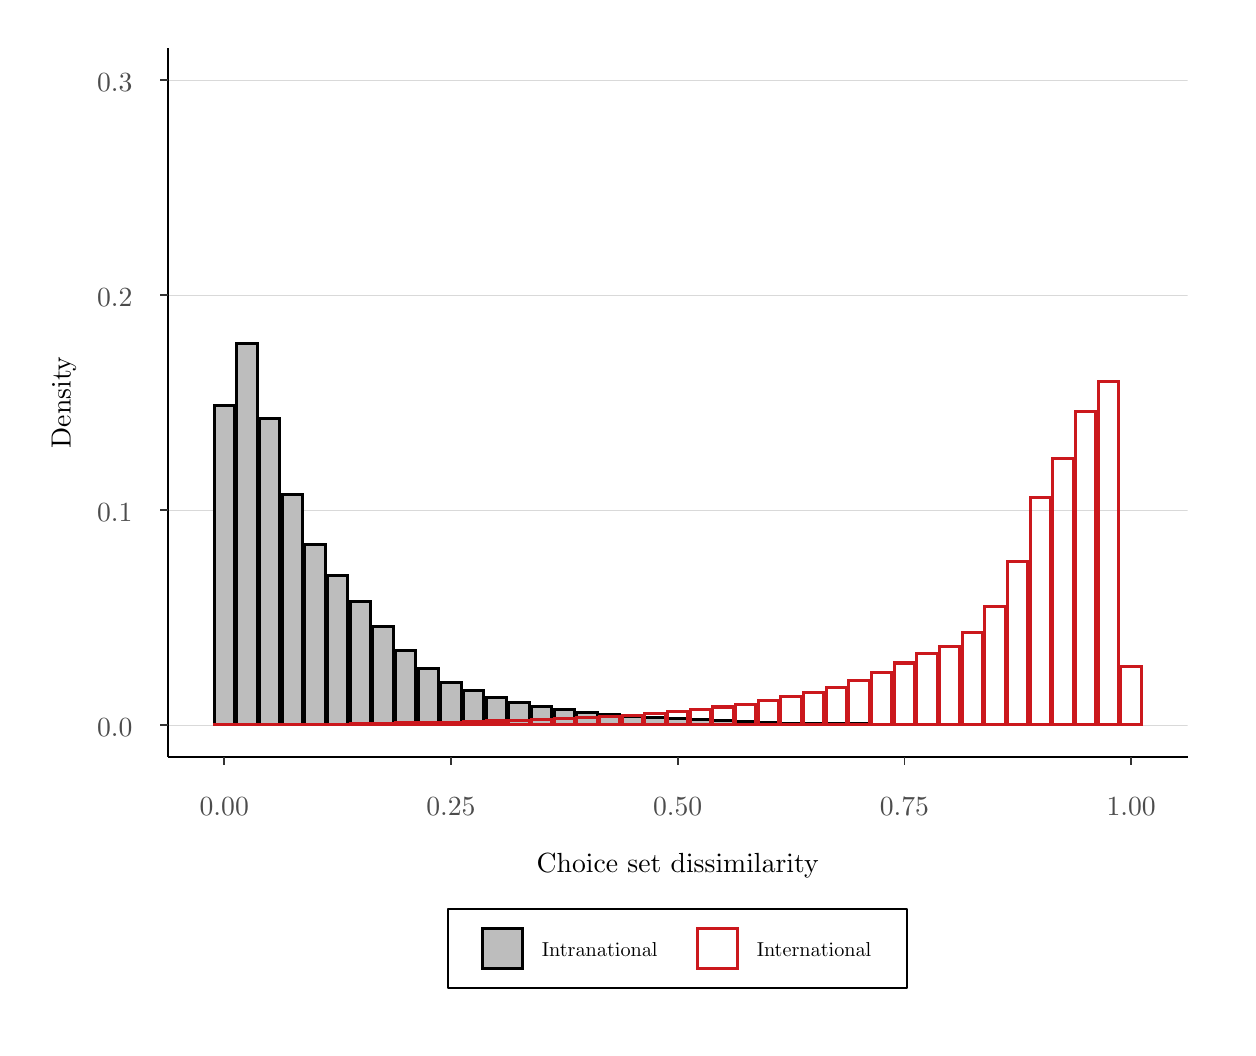
\begin{tikzpicture}[x=1pt,y=1pt]
\definecolor{fillColor}{RGB}{255,255,255}
\path[use as bounding box,fill=fillColor,fill opacity=0.00] (0,0) rectangle (433.62,361.35);
\begin{scope}
\path[clip] (  0.00,  0.00) rectangle (433.62,361.35);
\definecolor{drawColor}{RGB}{255,255,255}
\definecolor{fillColor}{RGB}{255,255,255}

\path[draw=drawColor,line width= 0.6pt,line join=round,line cap=round,fill=fillColor] (  0.00,  0.00) rectangle (433.62,361.35);
\end{scope}
\begin{scope}
\path[clip] ( 50.59, 97.75) rectangle (419.17,354.12);
\definecolor{drawColor}{RGB}{255,255,255}

\path[draw=drawColor,line width= 0.3pt,line join=round] ( 50.59,148.25) --
	(419.17,148.25);

\path[draw=drawColor,line width= 0.3pt,line join=round] ( 50.59,225.94) --
	(419.17,225.94);

\path[draw=drawColor,line width= 0.3pt,line join=round] ( 50.59,303.62) --
	(419.17,303.62);

\path[draw=drawColor,line width= 0.3pt,line join=round] (111.99, 97.75) --
	(111.99,354.12);

\path[draw=drawColor,line width= 0.3pt,line join=round] (193.92, 97.75) --
	(193.92,354.12);

\path[draw=drawColor,line width= 0.3pt,line join=round] (275.84, 97.75) --
	(275.84,354.12);

\path[draw=drawColor,line width= 0.3pt,line join=round] (357.76, 97.75) --
	(357.76,354.12);
\definecolor{drawColor}{gray}{0.85}

\path[draw=drawColor,line width= 0.1pt,line join=round] ( 50.59,109.40) --
	(419.17,109.40);

\path[draw=drawColor,line width= 0.1pt,line join=round] ( 50.59,187.09) --
	(419.17,187.09);

\path[draw=drawColor,line width= 0.1pt,line join=round] ( 50.59,264.78) --
	(419.17,264.78);

\path[draw=drawColor,line width= 0.1pt,line join=round] ( 50.59,342.47) --
	(419.17,342.47);
\definecolor{drawColor}{RGB}{0,0,0}
\definecolor{fillColor}{gray}{0.74}

\path[draw=drawColor,line width= 1.1pt,line cap=rect,fill=fillColor] ( 67.34,109.40) rectangle ( 74.72,224.75);
\definecolor{drawColor}{RGB}{203,24,29}

\path[draw=drawColor,line width= 1.1pt,line cap=rect] ( 67.34,109.40) rectangle ( 74.72,109.41);
\definecolor{drawColor}{RGB}{0,0,0}

\path[draw=drawColor,line width= 1.1pt,line cap=rect,fill=fillColor] ( 75.54,109.40) rectangle ( 82.91,247.28);
\definecolor{drawColor}{RGB}{203,24,29}

\path[draw=drawColor,line width= 1.1pt,line cap=rect] ( 75.54,109.40) rectangle ( 82.91,109.48);
\definecolor{drawColor}{RGB}{0,0,0}

\path[draw=drawColor,line width= 1.1pt,line cap=rect,fill=fillColor] ( 83.73,109.40) rectangle ( 91.10,220.14);
\definecolor{drawColor}{RGB}{203,24,29}

\path[draw=drawColor,line width= 1.1pt,line cap=rect] ( 83.73,109.40) rectangle ( 91.10,109.52);
\definecolor{drawColor}{RGB}{0,0,0}

\path[draw=drawColor,line width= 1.1pt,line cap=rect,fill=fillColor] ( 91.92,109.40) rectangle ( 99.29,192.63);
\definecolor{drawColor}{RGB}{203,24,29}

\path[draw=drawColor,line width= 1.1pt,line cap=rect] ( 91.92,109.40) rectangle ( 99.29,109.58);
\definecolor{drawColor}{RGB}{0,0,0}

\path[draw=drawColor,line width= 1.1pt,line cap=rect,fill=fillColor] (100.11,109.40) rectangle (107.49,174.64);
\definecolor{drawColor}{RGB}{203,24,29}

\path[draw=drawColor,line width= 1.1pt,line cap=rect] (100.11,109.40) rectangle (107.49,109.63);
\definecolor{drawColor}{RGB}{0,0,0}

\path[draw=drawColor,line width= 1.1pt,line cap=rect,fill=fillColor] (108.31,109.40) rectangle (115.68,163.34);
\definecolor{drawColor}{RGB}{203,24,29}

\path[draw=drawColor,line width= 1.1pt,line cap=rect] (108.31,109.40) rectangle (115.68,109.71);
\definecolor{drawColor}{RGB}{0,0,0}

\path[draw=drawColor,line width= 1.1pt,line cap=rect,fill=fillColor] (116.50,109.40) rectangle (123.87,153.97);
\definecolor{drawColor}{RGB}{203,24,29}

\path[draw=drawColor,line width= 1.1pt,line cap=rect] (116.50,109.40) rectangle (123.87,109.83);
\definecolor{drawColor}{RGB}{0,0,0}

\path[draw=drawColor,line width= 1.1pt,line cap=rect,fill=fillColor] (124.69,109.40) rectangle (132.06,144.86);
\definecolor{drawColor}{RGB}{203,24,29}

\path[draw=drawColor,line width= 1.1pt,line cap=rect] (124.69,109.40) rectangle (132.06,109.92);
\definecolor{drawColor}{RGB}{0,0,0}

\path[draw=drawColor,line width= 1.1pt,line cap=rect,fill=fillColor] (132.88,109.40) rectangle (140.26,136.40);
\definecolor{drawColor}{RGB}{203,24,29}

\path[draw=drawColor,line width= 1.1pt,line cap=rect] (132.88,109.40) rectangle (140.26,110.09);
\definecolor{drawColor}{RGB}{0,0,0}

\path[draw=drawColor,line width= 1.1pt,line cap=rect,fill=fillColor] (141.08,109.40) rectangle (148.45,129.74);
\definecolor{drawColor}{RGB}{203,24,29}

\path[draw=drawColor,line width= 1.1pt,line cap=rect] (141.08,109.40) rectangle (148.45,110.27);
\definecolor{drawColor}{RGB}{0,0,0}

\path[draw=drawColor,line width= 1.1pt,line cap=rect,fill=fillColor] (149.27,109.40) rectangle (156.64,124.84);
\definecolor{drawColor}{RGB}{203,24,29}

\path[draw=drawColor,line width= 1.1pt,line cap=rect] (149.27,109.40) rectangle (156.64,110.44);
\definecolor{drawColor}{RGB}{0,0,0}

\path[draw=drawColor,line width= 1.1pt,line cap=rect,fill=fillColor] (157.46,109.40) rectangle (164.83,121.85);
\definecolor{drawColor}{RGB}{203,24,29}

\path[draw=drawColor,line width= 1.1pt,line cap=rect] (157.46,109.40) rectangle (164.83,110.65);
\definecolor{drawColor}{RGB}{0,0,0}

\path[draw=drawColor,line width= 1.1pt,line cap=rect,fill=fillColor] (165.65,109.40) rectangle (173.03,119.47);
\definecolor{drawColor}{RGB}{203,24,29}

\path[draw=drawColor,line width= 1.1pt,line cap=rect] (165.65,109.40) rectangle (173.03,110.81);
\definecolor{drawColor}{RGB}{0,0,0}

\path[draw=drawColor,line width= 1.1pt,line cap=rect,fill=fillColor] (173.85,109.40) rectangle (181.22,117.54);
\definecolor{drawColor}{RGB}{203,24,29}

\path[draw=drawColor,line width= 1.1pt,line cap=rect] (173.85,109.40) rectangle (181.22,111.01);
\definecolor{drawColor}{RGB}{0,0,0}

\path[draw=drawColor,line width= 1.1pt,line cap=rect,fill=fillColor] (182.04,109.40) rectangle (189.41,116.15);
\definecolor{drawColor}{RGB}{203,24,29}

\path[draw=drawColor,line width= 1.1pt,line cap=rect] (182.04,109.40) rectangle (189.41,111.24);
\definecolor{drawColor}{RGB}{0,0,0}

\path[draw=drawColor,line width= 1.1pt,line cap=rect,fill=fillColor] (190.23,109.40) rectangle (197.60,114.95);
\definecolor{drawColor}{RGB}{203,24,29}

\path[draw=drawColor,line width= 1.1pt,line cap=rect] (190.23,109.40) rectangle (197.60,111.56);
\definecolor{drawColor}{RGB}{0,0,0}

\path[draw=drawColor,line width= 1.1pt,line cap=rect,fill=fillColor] (198.42,109.40) rectangle (205.80,113.82);
\definecolor{drawColor}{RGB}{203,24,29}

\path[draw=drawColor,line width= 1.1pt,line cap=rect] (198.42,109.40) rectangle (205.80,111.93);
\definecolor{drawColor}{RGB}{0,0,0}

\path[draw=drawColor,line width= 1.1pt,line cap=rect,fill=fillColor] (206.61,109.40) rectangle (213.99,113.03);
\definecolor{drawColor}{RGB}{203,24,29}

\path[draw=drawColor,line width= 1.1pt,line cap=rect] (206.61,109.40) rectangle (213.99,112.33);
\definecolor{drawColor}{RGB}{0,0,0}

\path[draw=drawColor,line width= 1.1pt,line cap=rect,fill=fillColor] (214.81,109.40) rectangle (222.18,112.46);
\definecolor{drawColor}{RGB}{203,24,29}

\path[draw=drawColor,line width= 1.1pt,line cap=rect] (214.81,109.40) rectangle (222.18,112.79);
\definecolor{drawColor}{RGB}{0,0,0}

\path[draw=drawColor,line width= 1.1pt,line cap=rect,fill=fillColor] (223.00,109.40) rectangle (230.37,112.09);
\definecolor{drawColor}{RGB}{203,24,29}

\path[draw=drawColor,line width= 1.1pt,line cap=rect] (223.00,109.40) rectangle (230.37,113.39);
\definecolor{drawColor}{RGB}{0,0,0}

\path[draw=drawColor,line width= 1.1pt,line cap=rect,fill=fillColor] (231.19,109.40) rectangle (238.56,111.76);
\definecolor{drawColor}{RGB}{203,24,29}

\path[draw=drawColor,line width= 1.1pt,line cap=rect] (231.19,109.40) rectangle (238.56,114.13);
\definecolor{drawColor}{RGB}{0,0,0}

\path[draw=drawColor,line width= 1.1pt,line cap=rect,fill=fillColor] (239.38,109.40) rectangle (246.76,111.45);
\definecolor{drawColor}{RGB}{203,24,29}

\path[draw=drawColor,line width= 1.1pt,line cap=rect] (239.38,109.40) rectangle (246.76,114.89);
\definecolor{drawColor}{RGB}{0,0,0}

\path[draw=drawColor,line width= 1.1pt,line cap=rect,fill=fillColor] (247.58,109.40) rectangle (254.95,111.06);
\definecolor{drawColor}{RGB}{203,24,29}

\path[draw=drawColor,line width= 1.1pt,line cap=rect] (247.58,109.40) rectangle (254.95,115.87);
\definecolor{drawColor}{RGB}{0,0,0}

\path[draw=drawColor,line width= 1.1pt,line cap=rect,fill=fillColor] (255.77,109.40) rectangle (263.14,110.71);
\definecolor{drawColor}{RGB}{203,24,29}

\path[draw=drawColor,line width= 1.1pt,line cap=rect] (255.77,109.40) rectangle (263.14,116.89);
\definecolor{drawColor}{RGB}{0,0,0}

\path[draw=drawColor,line width= 1.1pt,line cap=rect,fill=fillColor] (263.96,109.40) rectangle (271.33,110.30);
\definecolor{drawColor}{RGB}{203,24,29}

\path[draw=drawColor,line width= 1.1pt,line cap=rect] (263.96,109.40) rectangle (271.33,118.10);
\definecolor{drawColor}{RGB}{0,0,0}

\path[draw=drawColor,line width= 1.1pt,line cap=rect,fill=fillColor] (272.15,109.40) rectangle (279.53,110.02);
\definecolor{drawColor}{RGB}{203,24,29}

\path[draw=drawColor,line width= 1.1pt,line cap=rect] (272.15,109.40) rectangle (279.53,119.55);
\definecolor{drawColor}{RGB}{0,0,0}

\path[draw=drawColor,line width= 1.1pt,line cap=rect,fill=fillColor] (280.35,109.40) rectangle (287.72,109.84);
\definecolor{drawColor}{RGB}{203,24,29}

\path[draw=drawColor,line width= 1.1pt,line cap=rect] (280.35,109.40) rectangle (287.72,121.07);
\definecolor{drawColor}{RGB}{0,0,0}

\path[draw=drawColor,line width= 1.1pt,line cap=rect,fill=fillColor] (288.54,109.40) rectangle (295.91,109.77);
\definecolor{drawColor}{RGB}{203,24,29}

\path[draw=drawColor,line width= 1.1pt,line cap=rect] (288.54,109.40) rectangle (295.91,122.96);
\definecolor{drawColor}{RGB}{0,0,0}

\path[draw=drawColor,line width= 1.1pt,line cap=rect,fill=fillColor] (296.73,109.40) rectangle (304.10,109.74);
\definecolor{drawColor}{RGB}{203,24,29}

\path[draw=drawColor,line width= 1.1pt,line cap=rect] (296.73,109.40) rectangle (304.10,125.38);
\definecolor{drawColor}{RGB}{0,0,0}

\path[draw=drawColor,line width= 1.1pt,line cap=rect,fill=fillColor] (304.92,109.40) rectangle (312.30,109.67);
\definecolor{drawColor}{RGB}{203,24,29}

\path[draw=drawColor,line width= 1.1pt,line cap=rect] (304.92,109.40) rectangle (312.30,128.24);
\definecolor{drawColor}{RGB}{0,0,0}

\path[draw=drawColor,line width= 1.1pt,line cap=rect,fill=fillColor] (313.12,109.40) rectangle (320.49,109.60);
\definecolor{drawColor}{RGB}{203,24,29}

\path[draw=drawColor,line width= 1.1pt,line cap=rect] (313.12,109.40) rectangle (320.49,131.77);
\definecolor{drawColor}{RGB}{0,0,0}

\path[draw=drawColor,line width= 1.1pt,line cap=rect,fill=fillColor] (321.31,109.40) rectangle (328.68,109.53);
\definecolor{drawColor}{RGB}{203,24,29}

\path[draw=drawColor,line width= 1.1pt,line cap=rect] (321.31,109.40) rectangle (328.68,135.07);
\definecolor{drawColor}{RGB}{0,0,0}

\path[draw=drawColor,line width= 1.1pt,line cap=rect,fill=fillColor] (329.50,109.40) rectangle (336.87,109.49);
\definecolor{drawColor}{RGB}{203,24,29}

\path[draw=drawColor,line width= 1.1pt,line cap=rect] (329.50,109.40) rectangle (336.87,137.80);
\definecolor{drawColor}{RGB}{0,0,0}

\path[draw=drawColor,line width= 1.1pt,line cap=rect,fill=fillColor] (337.69,109.40) rectangle (345.07,109.47);
\definecolor{drawColor}{RGB}{203,24,29}

\path[draw=drawColor,line width= 1.1pt,line cap=rect] (337.69,109.40) rectangle (345.07,142.70);
\definecolor{drawColor}{RGB}{0,0,0}

\path[draw=drawColor,line width= 1.1pt,line cap=rect,fill=fillColor] (345.89,109.40) rectangle (353.26,109.49);
\definecolor{drawColor}{RGB}{203,24,29}

\path[draw=drawColor,line width= 1.1pt,line cap=rect] (345.89,109.40) rectangle (353.26,152.13);
\definecolor{drawColor}{RGB}{0,0,0}

\path[draw=drawColor,line width= 1.1pt,line cap=rect,fill=fillColor] (354.08,109.40) rectangle (361.45,109.47);
\definecolor{drawColor}{RGB}{203,24,29}

\path[draw=drawColor,line width= 1.1pt,line cap=rect] (354.08,109.40) rectangle (361.45,168.54);
\definecolor{drawColor}{RGB}{0,0,0}

\path[draw=drawColor,line width= 1.1pt,line cap=rect,fill=fillColor] (362.27,109.40) rectangle (369.64,109.44);
\definecolor{drawColor}{RGB}{203,24,29}

\path[draw=drawColor,line width= 1.1pt,line cap=rect] (362.27,109.40) rectangle (369.64,191.48);
\definecolor{drawColor}{RGB}{0,0,0}

\path[draw=drawColor,line width= 1.1pt,line cap=rect,fill=fillColor] (370.46,109.40) rectangle (377.84,109.42);
\definecolor{drawColor}{RGB}{203,24,29}

\path[draw=drawColor,line width= 1.1pt,line cap=rect] (370.46,109.40) rectangle (377.84,205.67);
\definecolor{drawColor}{RGB}{0,0,0}

\path[draw=drawColor,line width= 1.1pt,line cap=rect,fill=fillColor] (378.65,109.40) rectangle (386.03,109.41);
\definecolor{drawColor}{RGB}{203,24,29}

\path[draw=drawColor,line width= 1.1pt,line cap=rect] (378.65,109.40) rectangle (386.03,222.62);

\path[draw=drawColor,line width= 1.1pt,line cap=rect] (386.85,109.40) rectangle (394.22,233.49);

\path[draw=drawColor,line width= 1.1pt,line cap=rect] (395.04,109.40) rectangle (402.41,130.40);
\end{scope}
\begin{scope}
\path[clip] (  0.00,  0.00) rectangle (433.62,361.35);
\definecolor{drawColor}{RGB}{0,0,0}

\path[draw=drawColor,line width= 0.6pt,line join=round] ( 50.59, 97.75) --
	( 50.59,354.12);
\end{scope}
\begin{scope}
\path[clip] (  0.00,  0.00) rectangle (433.62,361.35);
\definecolor{drawColor}{gray}{0.30}

\node[text=drawColor,anchor=base east,inner sep=0pt, outer sep=0pt, scale=  1.00] at ( 37.84,105.27) {0.0};

\node[text=drawColor,anchor=base east,inner sep=0pt, outer sep=0pt, scale=  1.00] at ( 37.84,182.96) {0.1};

\node[text=drawColor,anchor=base east,inner sep=0pt, outer sep=0pt, scale=  1.00] at ( 37.84,260.65) {0.2};

\node[text=drawColor,anchor=base east,inner sep=0pt, outer sep=0pt, scale=  1.00] at ( 37.84,338.34) {0.3};
\end{scope}
\begin{scope}
\path[clip] (  0.00,  0.00) rectangle (433.62,361.35);
\definecolor{drawColor}{gray}{0.20}

\path[draw=drawColor,line width= 0.6pt,line join=round] ( 47.84,109.40) --
	( 50.59,109.40);

\path[draw=drawColor,line width= 0.6pt,line join=round] ( 47.84,187.09) --
	( 50.59,187.09);

\path[draw=drawColor,line width= 0.6pt,line join=round] ( 47.84,264.78) --
	( 50.59,264.78);

\path[draw=drawColor,line width= 0.6pt,line join=round] ( 47.84,342.47) --
	( 50.59,342.47);
\end{scope}
\begin{scope}
\path[clip] (  0.00,  0.00) rectangle (433.62,361.35);
\definecolor{drawColor}{RGB}{0,0,0}

\path[draw=drawColor,line width= 0.6pt,line join=round] ( 50.59, 97.75) --
	(419.17, 97.75);
\end{scope}
\begin{scope}
\path[clip] (  0.00,  0.00) rectangle (433.62,361.35);
\definecolor{drawColor}{gray}{0.20}

\path[draw=drawColor,line width= 0.6pt,line join=round] ( 71.03, 95.00) --
	( 71.03, 97.75);

\path[draw=drawColor,line width= 0.6pt,line join=round] (152.95, 95.00) --
	(152.95, 97.75);

\path[draw=drawColor,line width= 0.6pt,line join=round] (234.88, 95.00) --
	(234.88, 97.75);

\path[draw=drawColor,line width= 0.6pt,line join=round] (316.80, 95.00) --
	(316.80, 97.75);

\path[draw=drawColor,line width= 0.6pt,line join=round] (398.73, 95.00) --
	(398.73, 97.75);
\end{scope}
\begin{scope}
\path[clip] (  0.00,  0.00) rectangle (433.62,361.35);
\definecolor{drawColor}{gray}{0.30}

\node[text=drawColor,anchor=base,inner sep=0pt, outer sep=0pt, scale=  1.00] at ( 71.03, 76.73) {0.00};

\node[text=drawColor,anchor=base,inner sep=0pt, outer sep=0pt, scale=  1.00] at (152.95, 76.73) {0.25};

\node[text=drawColor,anchor=base,inner sep=0pt, outer sep=0pt, scale=  1.00] at (234.88, 76.73) {0.50};

\node[text=drawColor,anchor=base,inner sep=0pt, outer sep=0pt, scale=  1.00] at (316.80, 76.73) {0.75};

\node[text=drawColor,anchor=base,inner sep=0pt, outer sep=0pt, scale=  1.00] at (398.73, 76.73) {1.00};
\end{scope}
\begin{scope}
\path[clip] (  0.00,  0.00) rectangle (433.62,361.35);
\definecolor{drawColor}{RGB}{0,0,0}

\node[text=drawColor,anchor=base,inner sep=0pt, outer sep=0pt, scale=  1.00] at (234.88, 56.13) {Choice set dissimilarity};
\end{scope}
\begin{scope}
\path[clip] (  0.00,  0.00) rectangle (433.62,361.35);
\definecolor{drawColor}{RGB}{0,0,0}

\node[text=drawColor,rotate= 90.00,anchor=base,inner sep=0pt, outer sep=0pt, scale=  1.00] at ( 15.49,225.94) {Density};
\end{scope}
\begin{scope}
\path[clip] (  0.00,  0.00) rectangle (433.62,361.35);
\definecolor{drawColor}{RGB}{0,0,0}
\definecolor{fillColor}{RGB}{255,255,255}

\path[draw=drawColor,line width= 0.6pt,line join=round,line cap=round,fill=fillColor] (151.97, 14.45) rectangle (317.79, 42.80);
\end{scope}
\begin{scope}
\path[clip] (  0.00,  0.00) rectangle (433.62,361.35);

\path[] (162.97, 19.95) rectangle (180.32, 37.30);
\end{scope}
\begin{scope}
\path[clip] (  0.00,  0.00) rectangle (433.62,361.35);
\definecolor{drawColor}{RGB}{0,0,0}
\definecolor{fillColor}{gray}{0.74}

\path[draw=drawColor,line width= 1.1pt,line cap=rect,fill=fillColor] (164.39, 21.38) rectangle (178.89, 35.88);
\end{scope}
\begin{scope}
\path[clip] (  0.00,  0.00) rectangle (433.62,361.35);

\path[] (240.62, 19.95) rectangle (257.96, 37.30);
\end{scope}
\begin{scope}
\path[clip] (  0.00,  0.00) rectangle (433.62,361.35);
\definecolor{drawColor}{RGB}{203,24,29}

\path[draw=drawColor,line width= 1.1pt,line cap=rect] (242.04, 21.38) rectangle (256.54, 35.88);
\end{scope}
\begin{scope}
\path[clip] (  0.00,  0.00) rectangle (433.62,361.35);
\definecolor{drawColor}{RGB}{0,0,0}

\node[text=drawColor,anchor=base west,inner sep=0pt, outer sep=0pt, scale=  0.73] at (185.82, 25.60) {Intranational};
\end{scope}
\begin{scope}
\path[clip] (  0.00,  0.00) rectangle (433.62,361.35);
\definecolor{drawColor}{RGB}{0,0,0}

\node[text=drawColor,anchor=base west,inner sep=0pt, outer sep=0pt, scale=  0.73] at (263.46, 25.60) {International};
\end{scope}
\end{tikzpicture}
}
     \end{subfigure}\\
     \begin{subfigure}[t]{.49\textwidth}
         \centering
         \caption{Household - $N^{B,ll'}_{p,t}$}
         \scalebox{0.45}{% Created by tikzDevice version 0.12.3.1 on 2022-10-03 21:44:13
% !TEX encoding = UTF-8 Unicode
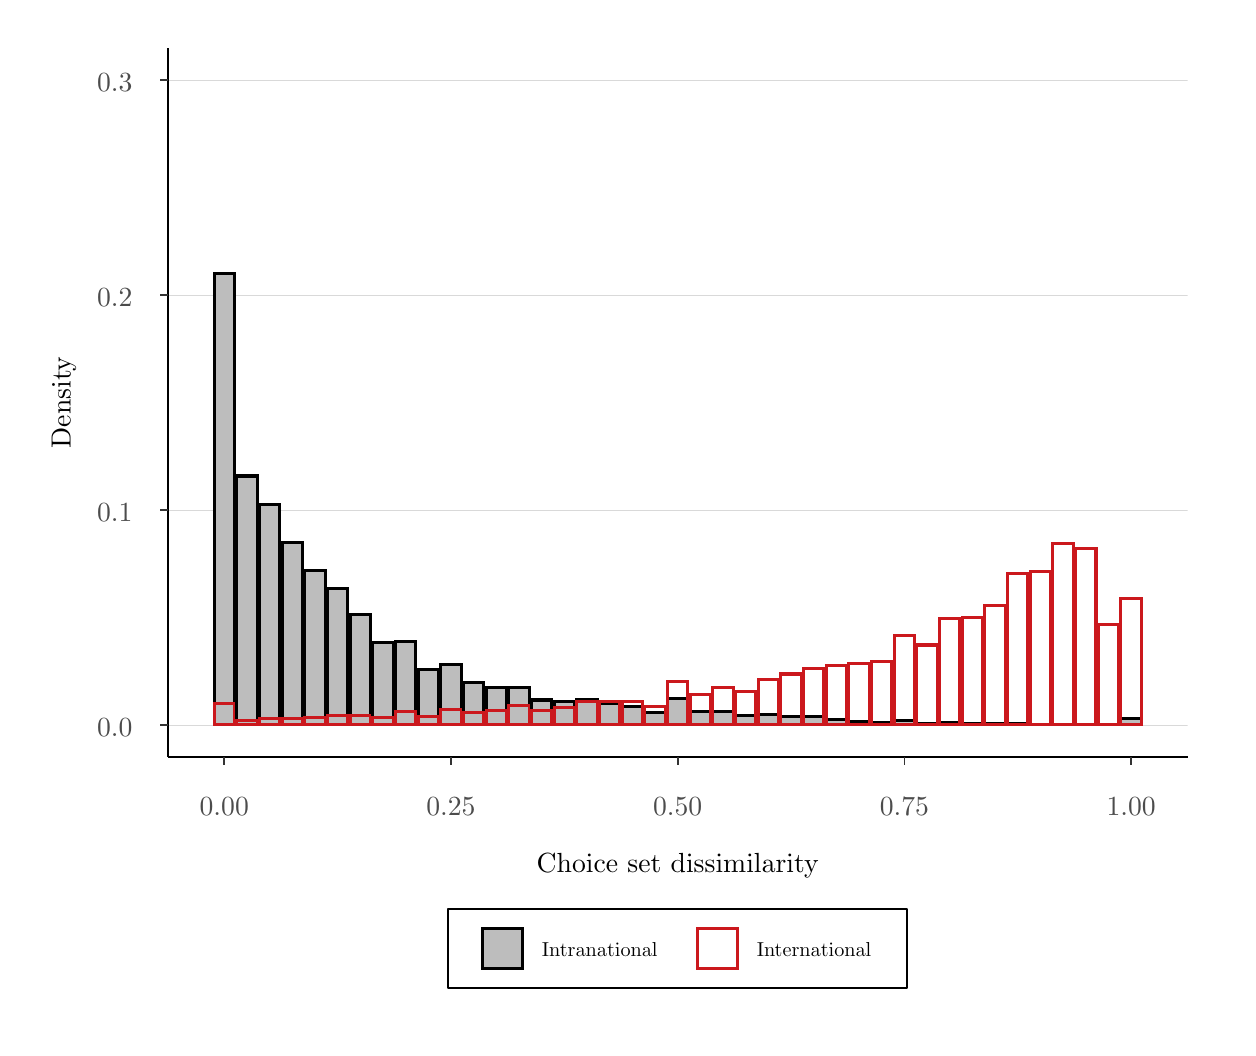
\begin{tikzpicture}[x=1pt,y=1pt]
\definecolor{fillColor}{RGB}{255,255,255}
\path[use as bounding box,fill=fillColor,fill opacity=0.00] (0,0) rectangle (433.62,361.35);
\begin{scope}
\path[clip] (  0.00,  0.00) rectangle (433.62,361.35);
\definecolor{drawColor}{RGB}{255,255,255}
\definecolor{fillColor}{RGB}{255,255,255}

\path[draw=drawColor,line width= 0.6pt,line join=round,line cap=round,fill=fillColor] (  0.00,  0.00) rectangle (433.62,361.35);
\end{scope}
\begin{scope}
\path[clip] ( 50.59, 97.75) rectangle (419.17,354.12);
\definecolor{drawColor}{RGB}{255,255,255}

\path[draw=drawColor,line width= 0.3pt,line join=round] ( 50.59,148.25) --
	(419.17,148.25);

\path[draw=drawColor,line width= 0.3pt,line join=round] ( 50.59,225.94) --
	(419.17,225.94);

\path[draw=drawColor,line width= 0.3pt,line join=round] ( 50.59,303.62) --
	(419.17,303.62);

\path[draw=drawColor,line width= 0.3pt,line join=round] (111.99, 97.75) --
	(111.99,354.12);

\path[draw=drawColor,line width= 0.3pt,line join=round] (193.92, 97.75) --
	(193.92,354.12);

\path[draw=drawColor,line width= 0.3pt,line join=round] (275.84, 97.75) --
	(275.84,354.12);

\path[draw=drawColor,line width= 0.3pt,line join=round] (357.76, 97.75) --
	(357.76,354.12);
\definecolor{drawColor}{gray}{0.85}

\path[draw=drawColor,line width= 0.1pt,line join=round] ( 50.59,109.40) --
	(419.17,109.40);

\path[draw=drawColor,line width= 0.1pt,line join=round] ( 50.59,187.09) --
	(419.17,187.09);

\path[draw=drawColor,line width= 0.1pt,line join=round] ( 50.59,264.78) --
	(419.17,264.78);

\path[draw=drawColor,line width= 0.1pt,line join=round] ( 50.59,342.47) --
	(419.17,342.47);
\definecolor{drawColor}{RGB}{0,0,0}
\definecolor{fillColor}{gray}{0.74}

\path[draw=drawColor,line width= 1.1pt,line cap=rect,fill=fillColor] ( 67.34,109.40) rectangle ( 74.72,272.66);
\definecolor{drawColor}{RGB}{203,24,29}

\path[draw=drawColor,line width= 1.1pt,line cap=rect] ( 67.34,109.40) rectangle ( 74.72,117.23);
\definecolor{drawColor}{RGB}{0,0,0}

\path[draw=drawColor,line width= 1.1pt,line cap=rect,fill=fillColor] ( 75.54,109.40) rectangle ( 82.91,199.34);
\definecolor{drawColor}{RGB}{203,24,29}

\path[draw=drawColor,line width= 1.1pt,line cap=rect] ( 75.54,109.40) rectangle ( 82.91,111.02);
\definecolor{drawColor}{RGB}{0,0,0}

\path[draw=drawColor,line width= 1.1pt,line cap=rect,fill=fillColor] ( 83.73,109.40) rectangle ( 91.10,189.08);
\definecolor{drawColor}{RGB}{203,24,29}

\path[draw=drawColor,line width= 1.1pt,line cap=rect] ( 83.73,109.40) rectangle ( 91.10,111.55);
\definecolor{drawColor}{RGB}{0,0,0}

\path[draw=drawColor,line width= 1.1pt,line cap=rect,fill=fillColor] ( 91.92,109.40) rectangle ( 99.29,175.35);
\definecolor{drawColor}{RGB}{203,24,29}

\path[draw=drawColor,line width= 1.1pt,line cap=rect] ( 91.92,109.40) rectangle ( 99.29,111.71);
\definecolor{drawColor}{RGB}{0,0,0}

\path[draw=drawColor,line width= 1.1pt,line cap=rect,fill=fillColor] (100.11,109.40) rectangle (107.49,165.29);
\definecolor{drawColor}{RGB}{203,24,29}

\path[draw=drawColor,line width= 1.1pt,line cap=rect] (100.11,109.40) rectangle (107.49,112.08);
\definecolor{drawColor}{RGB}{0,0,0}

\path[draw=drawColor,line width= 1.1pt,line cap=rect,fill=fillColor] (108.31,109.40) rectangle (115.68,158.56);
\definecolor{drawColor}{RGB}{203,24,29}

\path[draw=drawColor,line width= 1.1pt,line cap=rect] (108.31,109.40) rectangle (115.68,112.74);
\definecolor{drawColor}{RGB}{0,0,0}

\path[draw=drawColor,line width= 1.1pt,line cap=rect,fill=fillColor] (116.50,109.40) rectangle (123.87,149.28);
\definecolor{drawColor}{RGB}{203,24,29}

\path[draw=drawColor,line width= 1.1pt,line cap=rect] (116.50,109.40) rectangle (123.87,112.86);
\definecolor{drawColor}{RGB}{0,0,0}

\path[draw=drawColor,line width= 1.1pt,line cap=rect,fill=fillColor] (124.69,109.40) rectangle (132.06,139.06);
\definecolor{drawColor}{RGB}{203,24,29}

\path[draw=drawColor,line width= 1.1pt,line cap=rect] (124.69,109.40) rectangle (132.06,112.21);
\definecolor{drawColor}{RGB}{0,0,0}

\path[draw=drawColor,line width= 1.1pt,line cap=rect,fill=fillColor] (132.88,109.40) rectangle (140.26,139.46);
\definecolor{drawColor}{RGB}{203,24,29}

\path[draw=drawColor,line width= 1.1pt,line cap=rect] (132.88,109.40) rectangle (140.26,114.12);
\definecolor{drawColor}{RGB}{0,0,0}

\path[draw=drawColor,line width= 1.1pt,line cap=rect,fill=fillColor] (141.08,109.40) rectangle (148.45,129.45);
\definecolor{drawColor}{RGB}{203,24,29}

\path[draw=drawColor,line width= 1.1pt,line cap=rect] (141.08,109.40) rectangle (148.45,112.51);
\definecolor{drawColor}{RGB}{0,0,0}

\path[draw=drawColor,line width= 1.1pt,line cap=rect,fill=fillColor] (149.27,109.40) rectangle (156.64,131.37);
\definecolor{drawColor}{RGB}{203,24,29}

\path[draw=drawColor,line width= 1.1pt,line cap=rect] (149.27,109.40) rectangle (156.64,115.13);
\definecolor{drawColor}{RGB}{0,0,0}

\path[draw=drawColor,line width= 1.1pt,line cap=rect,fill=fillColor] (157.46,109.40) rectangle (164.83,124.71);
\definecolor{drawColor}{RGB}{203,24,29}

\path[draw=drawColor,line width= 1.1pt,line cap=rect] (157.46,109.40) rectangle (164.83,113.88);
\definecolor{drawColor}{RGB}{0,0,0}

\path[draw=drawColor,line width= 1.1pt,line cap=rect,fill=fillColor] (165.65,109.40) rectangle (173.03,122.99);
\definecolor{drawColor}{RGB}{203,24,29}

\path[draw=drawColor,line width= 1.1pt,line cap=rect] (165.65,109.40) rectangle (173.03,114.54);
\definecolor{drawColor}{RGB}{0,0,0}

\path[draw=drawColor,line width= 1.1pt,line cap=rect,fill=fillColor] (173.85,109.40) rectangle (181.22,122.86);
\definecolor{drawColor}{RGB}{203,24,29}

\path[draw=drawColor,line width= 1.1pt,line cap=rect] (173.85,109.40) rectangle (181.22,116.48);
\definecolor{drawColor}{RGB}{0,0,0}

\path[draw=drawColor,line width= 1.1pt,line cap=rect,fill=fillColor] (182.04,109.40) rectangle (189.41,118.41);
\definecolor{drawColor}{RGB}{203,24,29}

\path[draw=drawColor,line width= 1.1pt,line cap=rect] (182.04,109.40) rectangle (189.41,114.71);
\definecolor{drawColor}{RGB}{0,0,0}

\path[draw=drawColor,line width= 1.1pt,line cap=rect,fill=fillColor] (190.23,109.40) rectangle (197.60,117.85);
\definecolor{drawColor}{RGB}{203,24,29}

\path[draw=drawColor,line width= 1.1pt,line cap=rect] (190.23,109.40) rectangle (197.60,115.71);
\definecolor{drawColor}{RGB}{0,0,0}

\path[draw=drawColor,line width= 1.1pt,line cap=rect,fill=fillColor] (198.42,109.40) rectangle (205.80,118.54);
\definecolor{drawColor}{RGB}{203,24,29}

\path[draw=drawColor,line width= 1.1pt,line cap=rect] (198.42,109.40) rectangle (205.80,117.73);
\definecolor{drawColor}{RGB}{0,0,0}

\path[draw=drawColor,line width= 1.1pt,line cap=rect,fill=fillColor] (206.61,109.40) rectangle (213.99,117.16);
\definecolor{drawColor}{RGB}{203,24,29}

\path[draw=drawColor,line width= 1.1pt,line cap=rect] (206.61,109.40) rectangle (213.99,117.88);
\definecolor{drawColor}{RGB}{0,0,0}

\path[draw=drawColor,line width= 1.1pt,line cap=rect,fill=fillColor] (214.81,109.40) rectangle (222.18,116.02);
\definecolor{drawColor}{RGB}{203,24,29}

\path[draw=drawColor,line width= 1.1pt,line cap=rect] (214.81,109.40) rectangle (222.18,117.78);
\definecolor{drawColor}{RGB}{0,0,0}

\path[draw=drawColor,line width= 1.1pt,line cap=rect,fill=fillColor] (223.00,109.40) rectangle (230.37,114.04);
\definecolor{drawColor}{RGB}{203,24,29}

\path[draw=drawColor,line width= 1.1pt,line cap=rect] (223.00,109.40) rectangle (230.37,115.91);
\definecolor{drawColor}{RGB}{0,0,0}

\path[draw=drawColor,line width= 1.1pt,line cap=rect,fill=fillColor] (231.19,109.40) rectangle (238.56,118.97);
\definecolor{drawColor}{RGB}{203,24,29}

\path[draw=drawColor,line width= 1.1pt,line cap=rect] (231.19,109.40) rectangle (238.56,125.17);
\definecolor{drawColor}{RGB}{0,0,0}

\path[draw=drawColor,line width= 1.1pt,line cap=rect,fill=fillColor] (239.38,109.40) rectangle (246.76,114.39);
\definecolor{drawColor}{RGB}{203,24,29}

\path[draw=drawColor,line width= 1.1pt,line cap=rect] (239.38,109.40) rectangle (246.76,120.46);
\definecolor{drawColor}{RGB}{0,0,0}

\path[draw=drawColor,line width= 1.1pt,line cap=rect,fill=fillColor] (247.58,109.40) rectangle (254.95,114.25);
\definecolor{drawColor}{RGB}{203,24,29}

\path[draw=drawColor,line width= 1.1pt,line cap=rect] (247.58,109.40) rectangle (254.95,122.85);
\definecolor{drawColor}{RGB}{0,0,0}

\path[draw=drawColor,line width= 1.1pt,line cap=rect,fill=fillColor] (255.77,109.40) rectangle (263.14,112.86);
\definecolor{drawColor}{RGB}{203,24,29}

\path[draw=drawColor,line width= 1.1pt,line cap=rect] (255.77,109.40) rectangle (263.14,121.52);
\definecolor{drawColor}{RGB}{0,0,0}

\path[draw=drawColor,line width= 1.1pt,line cap=rect,fill=fillColor] (263.96,109.40) rectangle (271.33,113.21);
\definecolor{drawColor}{RGB}{203,24,29}

\path[draw=drawColor,line width= 1.1pt,line cap=rect] (263.96,109.40) rectangle (271.33,125.85);
\definecolor{drawColor}{RGB}{0,0,0}

\path[draw=drawColor,line width= 1.1pt,line cap=rect,fill=fillColor] (272.15,109.40) rectangle (279.53,112.52);
\definecolor{drawColor}{RGB}{203,24,29}

\path[draw=drawColor,line width= 1.1pt,line cap=rect] (272.15,109.40) rectangle (279.53,127.80);
\definecolor{drawColor}{RGB}{0,0,0}

\path[draw=drawColor,line width= 1.1pt,line cap=rect,fill=fillColor] (280.35,109.40) rectangle (287.72,112.43);
\definecolor{drawColor}{RGB}{203,24,29}

\path[draw=drawColor,line width= 1.1pt,line cap=rect] (280.35,109.40) rectangle (287.72,129.77);
\definecolor{drawColor}{RGB}{0,0,0}

\path[draw=drawColor,line width= 1.1pt,line cap=rect,fill=fillColor] (288.54,109.40) rectangle (295.91,111.19);
\definecolor{drawColor}{RGB}{203,24,29}

\path[draw=drawColor,line width= 1.1pt,line cap=rect] (288.54,109.40) rectangle (295.91,130.80);
\definecolor{drawColor}{RGB}{0,0,0}

\path[draw=drawColor,line width= 1.1pt,line cap=rect,fill=fillColor] (296.73,109.40) rectangle (304.10,110.75);
\definecolor{drawColor}{RGB}{203,24,29}

\path[draw=drawColor,line width= 1.1pt,line cap=rect] (296.73,109.40) rectangle (304.10,131.57);
\definecolor{drawColor}{RGB}{0,0,0}

\path[draw=drawColor,line width= 1.1pt,line cap=rect,fill=fillColor] (304.92,109.40) rectangle (312.30,110.37);
\definecolor{drawColor}{RGB}{203,24,29}

\path[draw=drawColor,line width= 1.1pt,line cap=rect] (304.92,109.40) rectangle (312.30,132.35);
\definecolor{drawColor}{RGB}{0,0,0}

\path[draw=drawColor,line width= 1.1pt,line cap=rect,fill=fillColor] (313.12,109.40) rectangle (320.49,110.85);
\definecolor{drawColor}{RGB}{203,24,29}

\path[draw=drawColor,line width= 1.1pt,line cap=rect] (313.12,109.40) rectangle (320.49,141.64);
\definecolor{drawColor}{RGB}{0,0,0}

\path[draw=drawColor,line width= 1.1pt,line cap=rect,fill=fillColor] (321.31,109.40) rectangle (328.68,110.02);
\definecolor{drawColor}{RGB}{203,24,29}

\path[draw=drawColor,line width= 1.1pt,line cap=rect] (321.31,109.40) rectangle (328.68,138.27);
\definecolor{drawColor}{RGB}{0,0,0}

\path[draw=drawColor,line width= 1.1pt,line cap=rect,fill=fillColor] (329.50,109.40) rectangle (336.87,110.26);
\definecolor{drawColor}{RGB}{203,24,29}

\path[draw=drawColor,line width= 1.1pt,line cap=rect] (329.50,109.40) rectangle (336.87,147.79);
\definecolor{drawColor}{RGB}{0,0,0}

\path[draw=drawColor,line width= 1.1pt,line cap=rect,fill=fillColor] (337.69,109.40) rectangle (345.07,109.92);
\definecolor{drawColor}{RGB}{203,24,29}

\path[draw=drawColor,line width= 1.1pt,line cap=rect] (337.69,109.40) rectangle (345.07,148.18);
\definecolor{drawColor}{RGB}{0,0,0}

\path[draw=drawColor,line width= 1.1pt,line cap=rect,fill=fillColor] (345.89,109.40) rectangle (353.26,109.75);
\definecolor{drawColor}{RGB}{203,24,29}

\path[draw=drawColor,line width= 1.1pt,line cap=rect] (345.89,109.40) rectangle (353.26,152.61);
\definecolor{drawColor}{RGB}{0,0,0}

\path[draw=drawColor,line width= 1.1pt,line cap=rect,fill=fillColor] (354.08,109.40) rectangle (361.45,109.76);
\definecolor{drawColor}{RGB}{203,24,29}

\path[draw=drawColor,line width= 1.1pt,line cap=rect] (354.08,109.40) rectangle (361.45,164.17);
\definecolor{drawColor}{RGB}{0,0,0}

\path[draw=drawColor,line width= 1.1pt,line cap=rect,fill=fillColor] (362.27,109.40) rectangle (369.64,109.53);
\definecolor{drawColor}{RGB}{203,24,29}

\path[draw=drawColor,line width= 1.1pt,line cap=rect] (362.27,109.40) rectangle (369.64,164.86);
\definecolor{drawColor}{RGB}{0,0,0}

\path[draw=drawColor,line width= 1.1pt,line cap=rect,fill=fillColor] (370.46,109.40) rectangle (377.84,109.48);
\definecolor{drawColor}{RGB}{203,24,29}

\path[draw=drawColor,line width= 1.1pt,line cap=rect] (370.46,109.40) rectangle (377.84,174.83);
\definecolor{drawColor}{RGB}{0,0,0}

\path[draw=drawColor,line width= 1.1pt,line cap=rect,fill=fillColor] (378.65,109.40) rectangle (386.03,109.42);
\definecolor{drawColor}{RGB}{203,24,29}

\path[draw=drawColor,line width= 1.1pt,line cap=rect] (378.65,109.40) rectangle (386.03,173.11);
\definecolor{drawColor}{RGB}{0,0,0}

\path[draw=drawColor,line width= 1.1pt,line cap=rect,fill=fillColor] (386.85,109.40) rectangle (394.22,109.40);
\definecolor{drawColor}{RGB}{203,24,29}

\path[draw=drawColor,line width= 1.1pt,line cap=rect] (386.85,109.40) rectangle (394.22,145.76);
\definecolor{drawColor}{RGB}{0,0,0}

\path[draw=drawColor,line width= 1.1pt,line cap=rect,fill=fillColor] (395.04,109.40) rectangle (402.41,111.57);
\definecolor{drawColor}{RGB}{203,24,29}

\path[draw=drawColor,line width= 1.1pt,line cap=rect] (395.04,109.40) rectangle (402.41,155.20);
\end{scope}
\begin{scope}
\path[clip] (  0.00,  0.00) rectangle (433.62,361.35);
\definecolor{drawColor}{RGB}{0,0,0}

\path[draw=drawColor,line width= 0.6pt,line join=round] ( 50.59, 97.75) --
	( 50.59,354.12);
\end{scope}
\begin{scope}
\path[clip] (  0.00,  0.00) rectangle (433.62,361.35);
\definecolor{drawColor}{gray}{0.30}

\node[text=drawColor,anchor=base east,inner sep=0pt, outer sep=0pt, scale=  1.00] at ( 37.84,105.27) {0.0};

\node[text=drawColor,anchor=base east,inner sep=0pt, outer sep=0pt, scale=  1.00] at ( 37.84,182.96) {0.1};

\node[text=drawColor,anchor=base east,inner sep=0pt, outer sep=0pt, scale=  1.00] at ( 37.84,260.65) {0.2};

\node[text=drawColor,anchor=base east,inner sep=0pt, outer sep=0pt, scale=  1.00] at ( 37.84,338.34) {0.3};
\end{scope}
\begin{scope}
\path[clip] (  0.00,  0.00) rectangle (433.62,361.35);
\definecolor{drawColor}{gray}{0.20}

\path[draw=drawColor,line width= 0.6pt,line join=round] ( 47.84,109.40) --
	( 50.59,109.40);

\path[draw=drawColor,line width= 0.6pt,line join=round] ( 47.84,187.09) --
	( 50.59,187.09);

\path[draw=drawColor,line width= 0.6pt,line join=round] ( 47.84,264.78) --
	( 50.59,264.78);

\path[draw=drawColor,line width= 0.6pt,line join=round] ( 47.84,342.47) --
	( 50.59,342.47);
\end{scope}
\begin{scope}
\path[clip] (  0.00,  0.00) rectangle (433.62,361.35);
\definecolor{drawColor}{RGB}{0,0,0}

\path[draw=drawColor,line width= 0.6pt,line join=round] ( 50.59, 97.75) --
	(419.17, 97.75);
\end{scope}
\begin{scope}
\path[clip] (  0.00,  0.00) rectangle (433.62,361.35);
\definecolor{drawColor}{gray}{0.20}

\path[draw=drawColor,line width= 0.6pt,line join=round] ( 71.03, 95.00) --
	( 71.03, 97.75);

\path[draw=drawColor,line width= 0.6pt,line join=round] (152.95, 95.00) --
	(152.95, 97.75);

\path[draw=drawColor,line width= 0.6pt,line join=round] (234.88, 95.00) --
	(234.88, 97.75);

\path[draw=drawColor,line width= 0.6pt,line join=round] (316.80, 95.00) --
	(316.80, 97.75);

\path[draw=drawColor,line width= 0.6pt,line join=round] (398.73, 95.00) --
	(398.73, 97.75);
\end{scope}
\begin{scope}
\path[clip] (  0.00,  0.00) rectangle (433.62,361.35);
\definecolor{drawColor}{gray}{0.30}

\node[text=drawColor,anchor=base,inner sep=0pt, outer sep=0pt, scale=  1.00] at ( 71.03, 76.73) {0.00};

\node[text=drawColor,anchor=base,inner sep=0pt, outer sep=0pt, scale=  1.00] at (152.95, 76.73) {0.25};

\node[text=drawColor,anchor=base,inner sep=0pt, outer sep=0pt, scale=  1.00] at (234.88, 76.73) {0.50};

\node[text=drawColor,anchor=base,inner sep=0pt, outer sep=0pt, scale=  1.00] at (316.80, 76.73) {0.75};

\node[text=drawColor,anchor=base,inner sep=0pt, outer sep=0pt, scale=  1.00] at (398.73, 76.73) {1.00};
\end{scope}
\begin{scope}
\path[clip] (  0.00,  0.00) rectangle (433.62,361.35);
\definecolor{drawColor}{RGB}{0,0,0}

\node[text=drawColor,anchor=base,inner sep=0pt, outer sep=0pt, scale=  1.00] at (234.88, 56.13) {Choice set dissimilarity};
\end{scope}
\begin{scope}
\path[clip] (  0.00,  0.00) rectangle (433.62,361.35);
\definecolor{drawColor}{RGB}{0,0,0}

\node[text=drawColor,rotate= 90.00,anchor=base,inner sep=0pt, outer sep=0pt, scale=  1.00] at ( 15.49,225.94) {Density};
\end{scope}
\begin{scope}
\path[clip] (  0.00,  0.00) rectangle (433.62,361.35);
\definecolor{drawColor}{RGB}{0,0,0}
\definecolor{fillColor}{RGB}{255,255,255}

\path[draw=drawColor,line width= 0.6pt,line join=round,line cap=round,fill=fillColor] (151.97, 14.45) rectangle (317.79, 42.80);
\end{scope}
\begin{scope}
\path[clip] (  0.00,  0.00) rectangle (433.62,361.35);

\path[] (162.97, 19.95) rectangle (180.32, 37.30);
\end{scope}
\begin{scope}
\path[clip] (  0.00,  0.00) rectangle (433.62,361.35);
\definecolor{drawColor}{RGB}{0,0,0}
\definecolor{fillColor}{gray}{0.74}

\path[draw=drawColor,line width= 1.1pt,line cap=rect,fill=fillColor] (164.39, 21.38) rectangle (178.89, 35.88);
\end{scope}
\begin{scope}
\path[clip] (  0.00,  0.00) rectangle (433.62,361.35);

\path[] (240.62, 19.95) rectangle (257.96, 37.30);
\end{scope}
\begin{scope}
\path[clip] (  0.00,  0.00) rectangle (433.62,361.35);
\definecolor{drawColor}{RGB}{203,24,29}

\path[draw=drawColor,line width= 1.1pt,line cap=rect] (242.04, 21.38) rectangle (256.54, 35.88);
\end{scope}
\begin{scope}
\path[clip] (  0.00,  0.00) rectangle (433.62,361.35);
\definecolor{drawColor}{RGB}{0,0,0}

\node[text=drawColor,anchor=base west,inner sep=0pt, outer sep=0pt, scale=  0.73] at (185.82, 25.60) {Intranational};
\end{scope}
\begin{scope}
\path[clip] (  0.00,  0.00) rectangle (433.62,361.35);
\definecolor{drawColor}{RGB}{0,0,0}

\node[text=drawColor,anchor=base west,inner sep=0pt, outer sep=0pt, scale=  0.73] at (263.46, 25.60) {International};
\end{scope}
\end{tikzpicture}
}
     \end{subfigure}
     \begin{subfigure}[t]{.49\textwidth}
         \centering
         \caption{Household - $\lambda^{B,ll'}_{p,t}$}
         \scalebox{0.45}{\input{figures/descriptives/P1_2_3_3_2_bar_n_s_na.tex}}
     \end{subfigure}
     \parbox{\textwidth}{
        \begin{spacing}{1} 
            {\footnotesize 
            \textit{Notes}: This figure plots the distributions for the product variety-level dissimilarity measure across NUTS2-region pairs. The grey bars plot the distribution for NUTS2-region pairs when the two NUTS2-region pairs belong to the same country. The red bars do the same for NUTS1-region pairs that do not belong to the same country. In panels (a) and (b), the unit of observation is at the product category-region $l$-region $l'$-year level. Panel (a) plots the count-based dissimilarity measure and panel (b) plots the expenditure-based dissimilarity measure. The unit of observation is at the household type-product category-region $l$-region $l'$-year level. Panel (c) and (d) do the same for firm-level dissimilarity measures. Note that panel (d) has two y-axes: the left y-axis scales with the different country region pairs and the right y-axis scales with the same country region pairs.}
        \end{spacing}}
 \end{figure} 

 \begin{figure}[H]
    \centering
    \caption{Choice set differences: Branded or Private label product varieties}
    \label{fig: app_redform_bar_bp}
    \begin{subfigure}[t]{.49\textwidth}
         \centering
         \caption{Pooled - $N^{B,ll'}_{p,t}$}
         \scalebox{0.45}{% Created by tikzDevice version 0.12.3.1 on 2022-10-03 21:44:12
% !TEX encoding = UTF-8 Unicode
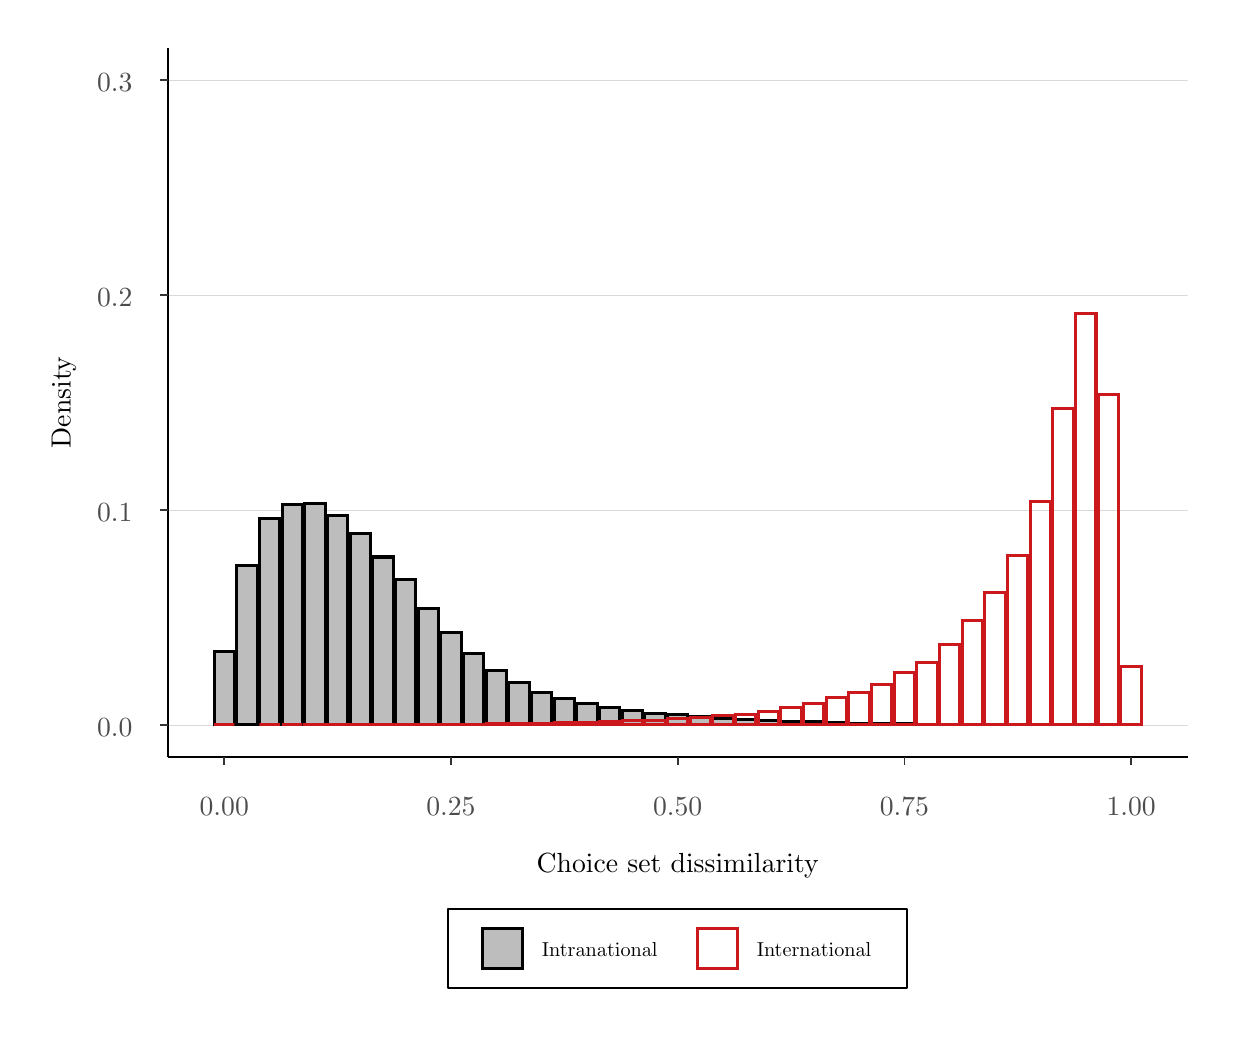
\begin{tikzpicture}[x=1pt,y=1pt]
\definecolor{fillColor}{RGB}{255,255,255}
\path[use as bounding box,fill=fillColor,fill opacity=0.00] (0,0) rectangle (433.62,361.35);
\begin{scope}
\path[clip] (  0.00,  0.00) rectangle (433.62,361.35);
\definecolor{drawColor}{RGB}{255,255,255}
\definecolor{fillColor}{RGB}{255,255,255}

\path[draw=drawColor,line width= 0.6pt,line join=round,line cap=round,fill=fillColor] (  0.00,  0.00) rectangle (433.62,361.35);
\end{scope}
\begin{scope}
\path[clip] ( 50.59, 97.75) rectangle (419.17,354.12);
\definecolor{drawColor}{RGB}{255,255,255}

\path[draw=drawColor,line width= 0.3pt,line join=round] ( 50.59,148.25) --
	(419.17,148.25);

\path[draw=drawColor,line width= 0.3pt,line join=round] ( 50.59,225.94) --
	(419.17,225.94);

\path[draw=drawColor,line width= 0.3pt,line join=round] ( 50.59,303.62) --
	(419.17,303.62);

\path[draw=drawColor,line width= 0.3pt,line join=round] (111.99, 97.75) --
	(111.99,354.12);

\path[draw=drawColor,line width= 0.3pt,line join=round] (193.92, 97.75) --
	(193.92,354.12);

\path[draw=drawColor,line width= 0.3pt,line join=round] (275.84, 97.75) --
	(275.84,354.12);

\path[draw=drawColor,line width= 0.3pt,line join=round] (357.76, 97.75) --
	(357.76,354.12);
\definecolor{drawColor}{gray}{0.85}

\path[draw=drawColor,line width= 0.1pt,line join=round] ( 50.59,109.40) --
	(419.17,109.40);

\path[draw=drawColor,line width= 0.1pt,line join=round] ( 50.59,187.09) --
	(419.17,187.09);

\path[draw=drawColor,line width= 0.1pt,line join=round] ( 50.59,264.78) --
	(419.17,264.78);

\path[draw=drawColor,line width= 0.1pt,line join=round] ( 50.59,342.47) --
	(419.17,342.47);
\definecolor{drawColor}{RGB}{0,0,0}
\definecolor{fillColor}{gray}{0.74}

\path[draw=drawColor,line width= 1.1pt,line cap=rect,fill=fillColor] ( 67.34,109.40) rectangle ( 74.72,136.09);
\definecolor{drawColor}{RGB}{203,24,29}

\path[draw=drawColor,line width= 1.1pt,line cap=rect] ( 67.34,109.40) rectangle ( 74.72,109.40);
\definecolor{drawColor}{RGB}{0,0,0}

\path[draw=drawColor,line width= 1.1pt,line cap=rect,fill=fillColor] ( 75.54,109.40) rectangle ( 82.91,167.13);

\path[draw=drawColor,line width= 1.1pt,line cap=rect,fill=fillColor] ( 83.73,109.40) rectangle ( 91.10,184.01);
\definecolor{drawColor}{RGB}{203,24,29}

\path[draw=drawColor,line width= 1.1pt,line cap=rect] ( 83.73,109.40) rectangle ( 91.10,109.40);
\definecolor{drawColor}{RGB}{0,0,0}

\path[draw=drawColor,line width= 1.1pt,line cap=rect,fill=fillColor] ( 91.92,109.40) rectangle ( 99.29,188.88);
\definecolor{drawColor}{RGB}{203,24,29}

\path[draw=drawColor,line width= 1.1pt,line cap=rect] ( 91.92,109.40) rectangle ( 99.29,109.40);
\definecolor{drawColor}{RGB}{0,0,0}

\path[draw=drawColor,line width= 1.1pt,line cap=rect,fill=fillColor] (100.11,109.40) rectangle (107.49,189.33);
\definecolor{drawColor}{RGB}{203,24,29}

\path[draw=drawColor,line width= 1.1pt,line cap=rect] (100.11,109.40) rectangle (107.49,109.41);
\definecolor{drawColor}{RGB}{0,0,0}

\path[draw=drawColor,line width= 1.1pt,line cap=rect,fill=fillColor] (108.31,109.40) rectangle (115.68,185.24);
\definecolor{drawColor}{RGB}{203,24,29}

\path[draw=drawColor,line width= 1.1pt,line cap=rect] (108.31,109.40) rectangle (115.68,109.41);
\definecolor{drawColor}{RGB}{0,0,0}

\path[draw=drawColor,line width= 1.1pt,line cap=rect,fill=fillColor] (116.50,109.40) rectangle (123.87,178.66);
\definecolor{drawColor}{RGB}{203,24,29}

\path[draw=drawColor,line width= 1.1pt,line cap=rect] (116.50,109.40) rectangle (123.87,109.42);
\definecolor{drawColor}{RGB}{0,0,0}

\path[draw=drawColor,line width= 1.1pt,line cap=rect,fill=fillColor] (124.69,109.40) rectangle (132.06,170.08);
\definecolor{drawColor}{RGB}{203,24,29}

\path[draw=drawColor,line width= 1.1pt,line cap=rect] (124.69,109.40) rectangle (132.06,109.44);
\definecolor{drawColor}{RGB}{0,0,0}

\path[draw=drawColor,line width= 1.1pt,line cap=rect,fill=fillColor] (132.88,109.40) rectangle (140.26,161.96);
\definecolor{drawColor}{RGB}{203,24,29}

\path[draw=drawColor,line width= 1.1pt,line cap=rect] (132.88,109.40) rectangle (140.26,109.47);
\definecolor{drawColor}{RGB}{0,0,0}

\path[draw=drawColor,line width= 1.1pt,line cap=rect,fill=fillColor] (141.08,109.40) rectangle (148.45,151.58);
\definecolor{drawColor}{RGB}{203,24,29}

\path[draw=drawColor,line width= 1.1pt,line cap=rect] (141.08,109.40) rectangle (148.45,109.49);
\definecolor{drawColor}{RGB}{0,0,0}

\path[draw=drawColor,line width= 1.1pt,line cap=rect,fill=fillColor] (149.27,109.40) rectangle (156.64,142.90);
\definecolor{drawColor}{RGB}{203,24,29}

\path[draw=drawColor,line width= 1.1pt,line cap=rect] (149.27,109.40) rectangle (156.64,109.55);
\definecolor{drawColor}{RGB}{0,0,0}

\path[draw=drawColor,line width= 1.1pt,line cap=rect,fill=fillColor] (157.46,109.40) rectangle (164.83,135.04);
\definecolor{drawColor}{RGB}{203,24,29}

\path[draw=drawColor,line width= 1.1pt,line cap=rect] (157.46,109.40) rectangle (164.83,109.61);
\definecolor{drawColor}{RGB}{0,0,0}

\path[draw=drawColor,line width= 1.1pt,line cap=rect,fill=fillColor] (165.65,109.40) rectangle (173.03,129.16);
\definecolor{drawColor}{RGB}{203,24,29}

\path[draw=drawColor,line width= 1.1pt,line cap=rect] (165.65,109.40) rectangle (173.03,109.74);
\definecolor{drawColor}{RGB}{0,0,0}

\path[draw=drawColor,line width= 1.1pt,line cap=rect,fill=fillColor] (173.85,109.40) rectangle (181.22,124.75);
\definecolor{drawColor}{RGB}{203,24,29}

\path[draw=drawColor,line width= 1.1pt,line cap=rect] (173.85,109.40) rectangle (181.22,109.88);
\definecolor{drawColor}{RGB}{0,0,0}

\path[draw=drawColor,line width= 1.1pt,line cap=rect,fill=fillColor] (182.04,109.40) rectangle (189.41,121.16);
\definecolor{drawColor}{RGB}{203,24,29}

\path[draw=drawColor,line width= 1.1pt,line cap=rect] (182.04,109.40) rectangle (189.41,109.99);
\definecolor{drawColor}{RGB}{0,0,0}

\path[draw=drawColor,line width= 1.1pt,line cap=rect,fill=fillColor] (190.23,109.40) rectangle (197.60,119.04);
\definecolor{drawColor}{RGB}{203,24,29}

\path[draw=drawColor,line width= 1.1pt,line cap=rect] (190.23,109.40) rectangle (197.60,110.19);
\definecolor{drawColor}{RGB}{0,0,0}

\path[draw=drawColor,line width= 1.1pt,line cap=rect,fill=fillColor] (198.42,109.40) rectangle (205.80,117.28);
\definecolor{drawColor}{RGB}{203,24,29}

\path[draw=drawColor,line width= 1.1pt,line cap=rect] (198.42,109.40) rectangle (205.80,110.39);
\definecolor{drawColor}{RGB}{0,0,0}

\path[draw=drawColor,line width= 1.1pt,line cap=rect,fill=fillColor] (206.61,109.40) rectangle (213.99,115.85);
\definecolor{drawColor}{RGB}{203,24,29}

\path[draw=drawColor,line width= 1.1pt,line cap=rect] (206.61,109.40) rectangle (213.99,110.61);
\definecolor{drawColor}{RGB}{0,0,0}

\path[draw=drawColor,line width= 1.1pt,line cap=rect,fill=fillColor] (214.81,109.40) rectangle (222.18,114.71);
\definecolor{drawColor}{RGB}{203,24,29}

\path[draw=drawColor,line width= 1.1pt,line cap=rect] (214.81,109.40) rectangle (222.18,110.94);
\definecolor{drawColor}{RGB}{0,0,0}

\path[draw=drawColor,line width= 1.1pt,line cap=rect,fill=fillColor] (223.00,109.40) rectangle (230.37,113.63);
\definecolor{drawColor}{RGB}{203,24,29}

\path[draw=drawColor,line width= 1.1pt,line cap=rect] (223.00,109.40) rectangle (230.37,111.13);
\definecolor{drawColor}{RGB}{0,0,0}

\path[draw=drawColor,line width= 1.1pt,line cap=rect,fill=fillColor] (231.19,109.40) rectangle (238.56,113.24);
\definecolor{drawColor}{RGB}{203,24,29}

\path[draw=drawColor,line width= 1.1pt,line cap=rect] (231.19,109.40) rectangle (238.56,111.82);
\definecolor{drawColor}{RGB}{0,0,0}

\path[draw=drawColor,line width= 1.1pt,line cap=rect,fill=fillColor] (239.38,109.40) rectangle (246.76,112.37);
\definecolor{drawColor}{RGB}{203,24,29}

\path[draw=drawColor,line width= 1.1pt,line cap=rect] (239.38,109.40) rectangle (246.76,112.12);
\definecolor{drawColor}{RGB}{0,0,0}

\path[draw=drawColor,line width= 1.1pt,line cap=rect,fill=fillColor] (247.58,109.40) rectangle (254.95,111.89);
\definecolor{drawColor}{RGB}{203,24,29}

\path[draw=drawColor,line width= 1.1pt,line cap=rect] (247.58,109.40) rectangle (254.95,112.69);
\definecolor{drawColor}{RGB}{0,0,0}

\path[draw=drawColor,line width= 1.1pt,line cap=rect,fill=fillColor] (255.77,109.40) rectangle (263.14,111.41);
\definecolor{drawColor}{RGB}{203,24,29}

\path[draw=drawColor,line width= 1.1pt,line cap=rect] (255.77,109.40) rectangle (263.14,113.31);
\definecolor{drawColor}{RGB}{0,0,0}

\path[draw=drawColor,line width= 1.1pt,line cap=rect,fill=fillColor] (263.96,109.40) rectangle (271.33,111.15);
\definecolor{drawColor}{RGB}{203,24,29}

\path[draw=drawColor,line width= 1.1pt,line cap=rect] (263.96,109.40) rectangle (271.33,114.40);
\definecolor{drawColor}{RGB}{0,0,0}

\path[draw=drawColor,line width= 1.1pt,line cap=rect,fill=fillColor] (272.15,109.40) rectangle (279.53,110.75);
\definecolor{drawColor}{RGB}{203,24,29}

\path[draw=drawColor,line width= 1.1pt,line cap=rect] (272.15,109.40) rectangle (279.53,115.56);
\definecolor{drawColor}{RGB}{0,0,0}

\path[draw=drawColor,line width= 1.1pt,line cap=rect,fill=fillColor] (280.35,109.40) rectangle (287.72,110.45);
\definecolor{drawColor}{RGB}{203,24,29}

\path[draw=drawColor,line width= 1.1pt,line cap=rect] (280.35,109.40) rectangle (287.72,117.10);
\definecolor{drawColor}{RGB}{0,0,0}

\path[draw=drawColor,line width= 1.1pt,line cap=rect,fill=fillColor] (288.54,109.40) rectangle (295.91,110.26);
\definecolor{drawColor}{RGB}{203,24,29}

\path[draw=drawColor,line width= 1.1pt,line cap=rect] (288.54,109.40) rectangle (295.91,119.17);
\definecolor{drawColor}{RGB}{0,0,0}

\path[draw=drawColor,line width= 1.1pt,line cap=rect,fill=fillColor] (296.73,109.40) rectangle (304.10,110.03);
\definecolor{drawColor}{RGB}{203,24,29}

\path[draw=drawColor,line width= 1.1pt,line cap=rect] (296.73,109.40) rectangle (304.10,121.26);
\definecolor{drawColor}{RGB}{0,0,0}

\path[draw=drawColor,line width= 1.1pt,line cap=rect,fill=fillColor] (304.92,109.40) rectangle (312.30,109.90);
\definecolor{drawColor}{RGB}{203,24,29}

\path[draw=drawColor,line width= 1.1pt,line cap=rect] (304.92,109.40) rectangle (312.30,124.04);
\definecolor{drawColor}{RGB}{0,0,0}

\path[draw=drawColor,line width= 1.1pt,line cap=rect,fill=fillColor] (313.12,109.40) rectangle (320.49,109.75);
\definecolor{drawColor}{RGB}{203,24,29}

\path[draw=drawColor,line width= 1.1pt,line cap=rect] (313.12,109.40) rectangle (320.49,128.29);
\definecolor{drawColor}{RGB}{0,0,0}

\path[draw=drawColor,line width= 1.1pt,line cap=rect,fill=fillColor] (321.31,109.40) rectangle (328.68,109.63);
\definecolor{drawColor}{RGB}{203,24,29}

\path[draw=drawColor,line width= 1.1pt,line cap=rect] (321.31,109.40) rectangle (328.68,132.00);
\definecolor{drawColor}{RGB}{0,0,0}

\path[draw=drawColor,line width= 1.1pt,line cap=rect,fill=fillColor] (329.50,109.40) rectangle (336.87,109.56);
\definecolor{drawColor}{RGB}{203,24,29}

\path[draw=drawColor,line width= 1.1pt,line cap=rect] (329.50,109.40) rectangle (336.87,138.59);
\definecolor{drawColor}{RGB}{0,0,0}

\path[draw=drawColor,line width= 1.1pt,line cap=rect,fill=fillColor] (337.69,109.40) rectangle (345.07,109.50);
\definecolor{drawColor}{RGB}{203,24,29}

\path[draw=drawColor,line width= 1.1pt,line cap=rect] (337.69,109.40) rectangle (345.07,147.03);
\definecolor{drawColor}{RGB}{0,0,0}

\path[draw=drawColor,line width= 1.1pt,line cap=rect,fill=fillColor] (345.89,109.40) rectangle (353.26,109.48);
\definecolor{drawColor}{RGB}{203,24,29}

\path[draw=drawColor,line width= 1.1pt,line cap=rect] (345.89,109.40) rectangle (353.26,157.29);
\definecolor{drawColor}{RGB}{0,0,0}

\path[draw=drawColor,line width= 1.1pt,line cap=rect,fill=fillColor] (354.08,109.40) rectangle (361.45,109.46);
\definecolor{drawColor}{RGB}{203,24,29}

\path[draw=drawColor,line width= 1.1pt,line cap=rect] (354.08,109.40) rectangle (361.45,170.52);
\definecolor{drawColor}{RGB}{0,0,0}

\path[draw=drawColor,line width= 1.1pt,line cap=rect,fill=fillColor] (362.27,109.40) rectangle (369.64,109.42);
\definecolor{drawColor}{RGB}{203,24,29}

\path[draw=drawColor,line width= 1.1pt,line cap=rect] (362.27,109.40) rectangle (369.64,190.06);
\definecolor{drawColor}{RGB}{0,0,0}

\path[draw=drawColor,line width= 1.1pt,line cap=rect,fill=fillColor] (370.46,109.40) rectangle (377.84,109.41);
\definecolor{drawColor}{RGB}{203,24,29}

\path[draw=drawColor,line width= 1.1pt,line cap=rect] (370.46,109.40) rectangle (377.84,223.69);

\path[draw=drawColor,line width= 1.1pt,line cap=rect] (378.65,109.40) rectangle (386.03,257.95);

\path[draw=drawColor,line width= 1.1pt,line cap=rect] (386.85,109.40) rectangle (394.22,228.75);

\path[draw=drawColor,line width= 1.1pt,line cap=rect] (395.04,109.40) rectangle (402.41,130.44);
\end{scope}
\begin{scope}
\path[clip] (  0.00,  0.00) rectangle (433.62,361.35);
\definecolor{drawColor}{RGB}{0,0,0}

\path[draw=drawColor,line width= 0.6pt,line join=round] ( 50.59, 97.75) --
	( 50.59,354.12);
\end{scope}
\begin{scope}
\path[clip] (  0.00,  0.00) rectangle (433.62,361.35);
\definecolor{drawColor}{gray}{0.30}

\node[text=drawColor,anchor=base east,inner sep=0pt, outer sep=0pt, scale=  1.00] at ( 37.84,105.27) {0.0};

\node[text=drawColor,anchor=base east,inner sep=0pt, outer sep=0pt, scale=  1.00] at ( 37.84,182.96) {0.1};

\node[text=drawColor,anchor=base east,inner sep=0pt, outer sep=0pt, scale=  1.00] at ( 37.84,260.65) {0.2};

\node[text=drawColor,anchor=base east,inner sep=0pt, outer sep=0pt, scale=  1.00] at ( 37.84,338.34) {0.3};
\end{scope}
\begin{scope}
\path[clip] (  0.00,  0.00) rectangle (433.62,361.35);
\definecolor{drawColor}{gray}{0.20}

\path[draw=drawColor,line width= 0.6pt,line join=round] ( 47.84,109.40) --
	( 50.59,109.40);

\path[draw=drawColor,line width= 0.6pt,line join=round] ( 47.84,187.09) --
	( 50.59,187.09);

\path[draw=drawColor,line width= 0.6pt,line join=round] ( 47.84,264.78) --
	( 50.59,264.78);

\path[draw=drawColor,line width= 0.6pt,line join=round] ( 47.84,342.47) --
	( 50.59,342.47);
\end{scope}
\begin{scope}
\path[clip] (  0.00,  0.00) rectangle (433.62,361.35);
\definecolor{drawColor}{RGB}{0,0,0}

\path[draw=drawColor,line width= 0.6pt,line join=round] ( 50.59, 97.75) --
	(419.17, 97.75);
\end{scope}
\begin{scope}
\path[clip] (  0.00,  0.00) rectangle (433.62,361.35);
\definecolor{drawColor}{gray}{0.20}

\path[draw=drawColor,line width= 0.6pt,line join=round] ( 71.03, 95.00) --
	( 71.03, 97.75);

\path[draw=drawColor,line width= 0.6pt,line join=round] (152.95, 95.00) --
	(152.95, 97.75);

\path[draw=drawColor,line width= 0.6pt,line join=round] (234.88, 95.00) --
	(234.88, 97.75);

\path[draw=drawColor,line width= 0.6pt,line join=round] (316.80, 95.00) --
	(316.80, 97.75);

\path[draw=drawColor,line width= 0.6pt,line join=round] (398.73, 95.00) --
	(398.73, 97.75);
\end{scope}
\begin{scope}
\path[clip] (  0.00,  0.00) rectangle (433.62,361.35);
\definecolor{drawColor}{gray}{0.30}

\node[text=drawColor,anchor=base,inner sep=0pt, outer sep=0pt, scale=  1.00] at ( 71.03, 76.73) {0.00};

\node[text=drawColor,anchor=base,inner sep=0pt, outer sep=0pt, scale=  1.00] at (152.95, 76.73) {0.25};

\node[text=drawColor,anchor=base,inner sep=0pt, outer sep=0pt, scale=  1.00] at (234.88, 76.73) {0.50};

\node[text=drawColor,anchor=base,inner sep=0pt, outer sep=0pt, scale=  1.00] at (316.80, 76.73) {0.75};

\node[text=drawColor,anchor=base,inner sep=0pt, outer sep=0pt, scale=  1.00] at (398.73, 76.73) {1.00};
\end{scope}
\begin{scope}
\path[clip] (  0.00,  0.00) rectangle (433.62,361.35);
\definecolor{drawColor}{RGB}{0,0,0}

\node[text=drawColor,anchor=base,inner sep=0pt, outer sep=0pt, scale=  1.00] at (234.88, 56.13) {Choice set dissimilarity};
\end{scope}
\begin{scope}
\path[clip] (  0.00,  0.00) rectangle (433.62,361.35);
\definecolor{drawColor}{RGB}{0,0,0}

\node[text=drawColor,rotate= 90.00,anchor=base,inner sep=0pt, outer sep=0pt, scale=  1.00] at ( 15.49,225.94) {Density};
\end{scope}
\begin{scope}
\path[clip] (  0.00,  0.00) rectangle (433.62,361.35);
\definecolor{drawColor}{RGB}{0,0,0}
\definecolor{fillColor}{RGB}{255,255,255}

\path[draw=drawColor,line width= 0.6pt,line join=round,line cap=round,fill=fillColor] (151.97, 14.45) rectangle (317.79, 42.80);
\end{scope}
\begin{scope}
\path[clip] (  0.00,  0.00) rectangle (433.62,361.35);

\path[] (162.97, 19.95) rectangle (180.32, 37.30);
\end{scope}
\begin{scope}
\path[clip] (  0.00,  0.00) rectangle (433.62,361.35);
\definecolor{drawColor}{RGB}{0,0,0}
\definecolor{fillColor}{gray}{0.74}

\path[draw=drawColor,line width= 1.1pt,line cap=rect,fill=fillColor] (164.39, 21.38) rectangle (178.89, 35.88);
\end{scope}
\begin{scope}
\path[clip] (  0.00,  0.00) rectangle (433.62,361.35);

\path[] (240.62, 19.95) rectangle (257.96, 37.30);
\end{scope}
\begin{scope}
\path[clip] (  0.00,  0.00) rectangle (433.62,361.35);
\definecolor{drawColor}{RGB}{203,24,29}

\path[draw=drawColor,line width= 1.1pt,line cap=rect] (242.04, 21.38) rectangle (256.54, 35.88);
\end{scope}
\begin{scope}
\path[clip] (  0.00,  0.00) rectangle (433.62,361.35);
\definecolor{drawColor}{RGB}{0,0,0}

\node[text=drawColor,anchor=base west,inner sep=0pt, outer sep=0pt, scale=  0.73] at (185.82, 25.60) {Intranational};
\end{scope}
\begin{scope}
\path[clip] (  0.00,  0.00) rectangle (433.62,361.35);
\definecolor{drawColor}{RGB}{0,0,0}

\node[text=drawColor,anchor=base west,inner sep=0pt, outer sep=0pt, scale=  0.73] at (263.46, 25.60) {International};
\end{scope}
\end{tikzpicture}
}
     \end{subfigure}
     \begin{subfigure}[t]{.49\textwidth}
         \centering
         \caption{Pooled - $\lambda^{B,ll'}_{p,t}$}
         \scalebox{0.45}{\input{figures/descriptives/P1_2_3_3_1_bar_n_s_na_bp.tex}}
     \end{subfigure}\\
     \begin{subfigure}[t]{.49\textwidth}
         \centering
         \caption{Household - $N^{B,ll'}_{p,t}$}
         \scalebox{0.45}{\input{figures/descriptives/P1_2_3_3_2_bar_n_n_na_bp.tex}}
     \end{subfigure}
     \begin{subfigure}[t]{.49\textwidth}
         \centering
         \caption{Household - $\lambda^{B,ll'}_{p,t}$}
         \scalebox{0.45}{\input{figures/descriptives/P1_2_3_3_2_bar_n_s_na_bp.tex}}
     \end{subfigure}
     \parbox{\textwidth}{
        \begin{spacing}{1} 
            {\footnotesize 
            \textit{Notes}: This figure plots the distributions for the product variety-level dissimilarity measure across NUTS2-region pairs. The grey bars plot the distribution for NUTS1-region pairs when the two NUTS2-region pairs belong to the same country. The red bars do the same for NUTS2-region pairs that do not belong to the same country. In panels (a) and (b), the unit of observation is at the product category-region $l$-region $l'$-year level. Panel (a) plots the count-based dissimilarity measure and panel (b) plots the expenditure-based dissimilarity measure. The unit of observation is at the household type-product category-region $l$-region $l'$-year level. Panel (c) and (d) do the same for firm-level dissimilarity measures. Note that panel (d) has two y-axes: the left y-axis scales with the different country region pairs and the right y-axis scales with the same country region pairs. We restrict the sample of product varieties to only branded or private-label product varieties.}
        \end{spacing}}
 \end{figure} 

 \begin{figure}[H]
    \centering
    \caption{Choice set differences: Branded product varieties}
    \label{fig: app_redform_bar_b}
    \begin{subfigure}[t]{.49\textwidth}
         \centering
         \caption{Pooled - $N^{B,ll'}_{p,t}$}
         \scalebox{0.45}{\input{figures/descriptives/P1_2_3_3_1_bar_n_n_na_b.tex}}
     \end{subfigure}
     \begin{subfigure}[t]{.49\textwidth}
         \centering
         \caption{Pooled - $\lambda^{B,ll'}_{p,t}$}
         \scalebox{0.45}{\input{figures/descriptives/P1_2_3_3_1_bar_n_s_na_b.tex}}
     \end{subfigure}\\
     \begin{subfigure}[t]{.49\textwidth}
         \centering
         \caption{Household - $N^{B,ll'}_{p,t}$}
         \scalebox{0.45}{% Created by tikzDevice version 0.12.3.1 on 2022-10-03 21:44:13
% !TEX encoding = UTF-8 Unicode
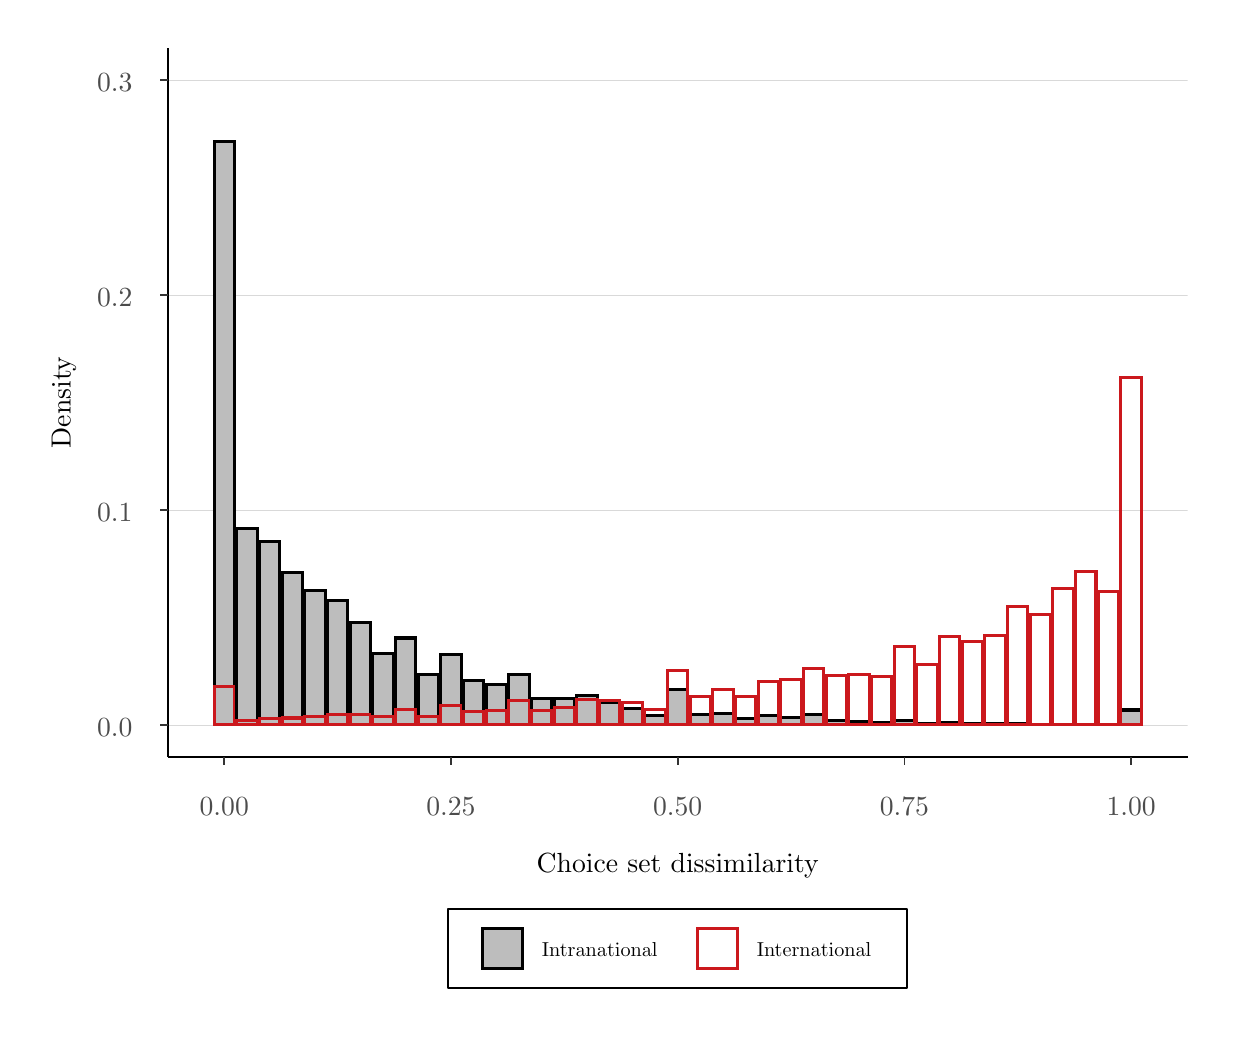
\begin{tikzpicture}[x=1pt,y=1pt]
\definecolor{fillColor}{RGB}{255,255,255}
\path[use as bounding box,fill=fillColor,fill opacity=0.00] (0,0) rectangle (433.62,361.35);
\begin{scope}
\path[clip] (  0.00,  0.00) rectangle (433.62,361.35);
\definecolor{drawColor}{RGB}{255,255,255}
\definecolor{fillColor}{RGB}{255,255,255}

\path[draw=drawColor,line width= 0.6pt,line join=round,line cap=round,fill=fillColor] (  0.00,  0.00) rectangle (433.62,361.35);
\end{scope}
\begin{scope}
\path[clip] ( 50.59, 97.75) rectangle (419.17,354.12);
\definecolor{drawColor}{RGB}{255,255,255}

\path[draw=drawColor,line width= 0.3pt,line join=round] ( 50.59,148.25) --
	(419.17,148.25);

\path[draw=drawColor,line width= 0.3pt,line join=round] ( 50.59,225.94) --
	(419.17,225.94);

\path[draw=drawColor,line width= 0.3pt,line join=round] ( 50.59,303.62) --
	(419.17,303.62);

\path[draw=drawColor,line width= 0.3pt,line join=round] (111.99, 97.75) --
	(111.99,354.12);

\path[draw=drawColor,line width= 0.3pt,line join=round] (193.92, 97.75) --
	(193.92,354.12);

\path[draw=drawColor,line width= 0.3pt,line join=round] (275.84, 97.75) --
	(275.84,354.12);

\path[draw=drawColor,line width= 0.3pt,line join=round] (357.76, 97.75) --
	(357.76,354.12);
\definecolor{drawColor}{gray}{0.85}

\path[draw=drawColor,line width= 0.1pt,line join=round] ( 50.59,109.40) --
	(419.17,109.40);

\path[draw=drawColor,line width= 0.1pt,line join=round] ( 50.59,187.09) --
	(419.17,187.09);

\path[draw=drawColor,line width= 0.1pt,line join=round] ( 50.59,264.78) --
	(419.17,264.78);

\path[draw=drawColor,line width= 0.1pt,line join=round] ( 50.59,342.47) --
	(419.17,342.47);
\definecolor{drawColor}{RGB}{0,0,0}
\definecolor{fillColor}{gray}{0.74}

\path[draw=drawColor,line width= 1.1pt,line cap=rect,fill=fillColor] ( 67.34,109.40) rectangle ( 74.72,320.32);
\definecolor{drawColor}{RGB}{203,24,29}

\path[draw=drawColor,line width= 1.1pt,line cap=rect] ( 67.34,109.40) rectangle ( 74.72,123.30);
\definecolor{drawColor}{RGB}{0,0,0}

\path[draw=drawColor,line width= 1.1pt,line cap=rect,fill=fillColor] ( 75.54,109.40) rectangle ( 82.91,180.29);
\definecolor{drawColor}{RGB}{203,24,29}

\path[draw=drawColor,line width= 1.1pt,line cap=rect] ( 75.54,109.40) rectangle ( 82.91,111.07);
\definecolor{drawColor}{RGB}{0,0,0}

\path[draw=drawColor,line width= 1.1pt,line cap=rect,fill=fillColor] ( 83.73,109.40) rectangle ( 91.10,175.56);
\definecolor{drawColor}{RGB}{203,24,29}

\path[draw=drawColor,line width= 1.1pt,line cap=rect] ( 83.73,109.40) rectangle ( 91.10,111.73);
\definecolor{drawColor}{RGB}{0,0,0}

\path[draw=drawColor,line width= 1.1pt,line cap=rect,fill=fillColor] ( 91.92,109.40) rectangle ( 99.29,164.33);
\definecolor{drawColor}{RGB}{203,24,29}

\path[draw=drawColor,line width= 1.1pt,line cap=rect] ( 91.92,109.40) rectangle ( 99.29,111.90);
\definecolor{drawColor}{RGB}{0,0,0}

\path[draw=drawColor,line width= 1.1pt,line cap=rect,fill=fillColor] (100.11,109.40) rectangle (107.49,158.08);
\definecolor{drawColor}{RGB}{203,24,29}

\path[draw=drawColor,line width= 1.1pt,line cap=rect] (100.11,109.40) rectangle (107.49,112.36);
\definecolor{drawColor}{RGB}{0,0,0}

\path[draw=drawColor,line width= 1.1pt,line cap=rect,fill=fillColor] (108.31,109.40) rectangle (115.68,154.33);
\definecolor{drawColor}{RGB}{203,24,29}

\path[draw=drawColor,line width= 1.1pt,line cap=rect] (108.31,109.40) rectangle (115.68,113.28);
\definecolor{drawColor}{RGB}{0,0,0}

\path[draw=drawColor,line width= 1.1pt,line cap=rect,fill=fillColor] (116.50,109.40) rectangle (123.87,146.25);
\definecolor{drawColor}{RGB}{203,24,29}

\path[draw=drawColor,line width= 1.1pt,line cap=rect] (116.50,109.40) rectangle (123.87,113.33);
\definecolor{drawColor}{RGB}{0,0,0}

\path[draw=drawColor,line width= 1.1pt,line cap=rect,fill=fillColor] (124.69,109.40) rectangle (132.06,135.21);
\definecolor{drawColor}{RGB}{203,24,29}

\path[draw=drawColor,line width= 1.1pt,line cap=rect] (124.69,109.40) rectangle (132.06,112.35);
\definecolor{drawColor}{RGB}{0,0,0}

\path[draw=drawColor,line width= 1.1pt,line cap=rect,fill=fillColor] (132.88,109.40) rectangle (140.26,140.80);
\definecolor{drawColor}{RGB}{203,24,29}

\path[draw=drawColor,line width= 1.1pt,line cap=rect] (132.88,109.40) rectangle (140.26,114.99);
\definecolor{drawColor}{RGB}{0,0,0}

\path[draw=drawColor,line width= 1.1pt,line cap=rect,fill=fillColor] (141.08,109.40) rectangle (148.45,127.50);
\definecolor{drawColor}{RGB}{203,24,29}

\path[draw=drawColor,line width= 1.1pt,line cap=rect] (141.08,109.40) rectangle (148.45,112.55);
\definecolor{drawColor}{RGB}{0,0,0}

\path[draw=drawColor,line width= 1.1pt,line cap=rect,fill=fillColor] (149.27,109.40) rectangle (156.64,134.68);
\definecolor{drawColor}{RGB}{203,24,29}

\path[draw=drawColor,line width= 1.1pt,line cap=rect] (149.27,109.40) rectangle (156.64,116.35);
\definecolor{drawColor}{RGB}{0,0,0}

\path[draw=drawColor,line width= 1.1pt,line cap=rect,fill=fillColor] (157.46,109.40) rectangle (164.83,125.38);
\definecolor{drawColor}{RGB}{203,24,29}

\path[draw=drawColor,line width= 1.1pt,line cap=rect] (157.46,109.40) rectangle (164.83,114.22);
\definecolor{drawColor}{RGB}{0,0,0}

\path[draw=drawColor,line width= 1.1pt,line cap=rect,fill=fillColor] (165.65,109.40) rectangle (173.03,123.85);
\definecolor{drawColor}{RGB}{203,24,29}

\path[draw=drawColor,line width= 1.1pt,line cap=rect] (165.65,109.40) rectangle (173.03,114.75);
\definecolor{drawColor}{RGB}{0,0,0}

\path[draw=drawColor,line width= 1.1pt,line cap=rect,fill=fillColor] (173.85,109.40) rectangle (181.22,127.57);
\definecolor{drawColor}{RGB}{203,24,29}

\path[draw=drawColor,line width= 1.1pt,line cap=rect] (173.85,109.40) rectangle (181.22,118.32);
\definecolor{drawColor}{RGB}{0,0,0}

\path[draw=drawColor,line width= 1.1pt,line cap=rect,fill=fillColor] (182.04,109.40) rectangle (189.41,119.10);
\definecolor{drawColor}{RGB}{203,24,29}

\path[draw=drawColor,line width= 1.1pt,line cap=rect] (182.04,109.40) rectangle (189.41,114.76);
\definecolor{drawColor}{RGB}{0,0,0}

\path[draw=drawColor,line width= 1.1pt,line cap=rect,fill=fillColor] (190.23,109.40) rectangle (197.60,118.92);
\definecolor{drawColor}{RGB}{203,24,29}

\path[draw=drawColor,line width= 1.1pt,line cap=rect] (190.23,109.40) rectangle (197.60,115.85);
\definecolor{drawColor}{RGB}{0,0,0}

\path[draw=drawColor,line width= 1.1pt,line cap=rect,fill=fillColor] (198.42,109.40) rectangle (205.80,120.03);
\definecolor{drawColor}{RGB}{203,24,29}

\path[draw=drawColor,line width= 1.1pt,line cap=rect] (198.42,109.40) rectangle (205.80,118.47);
\definecolor{drawColor}{RGB}{0,0,0}

\path[draw=drawColor,line width= 1.1pt,line cap=rect,fill=fillColor] (206.61,109.40) rectangle (213.99,117.58);
\definecolor{drawColor}{RGB}{203,24,29}

\path[draw=drawColor,line width= 1.1pt,line cap=rect] (206.61,109.40) rectangle (213.99,118.24);
\definecolor{drawColor}{RGB}{0,0,0}

\path[draw=drawColor,line width= 1.1pt,line cap=rect,fill=fillColor] (214.81,109.40) rectangle (222.18,115.38);
\definecolor{drawColor}{RGB}{203,24,29}

\path[draw=drawColor,line width= 1.1pt,line cap=rect] (214.81,109.40) rectangle (222.18,117.50);
\definecolor{drawColor}{RGB}{0,0,0}

\path[draw=drawColor,line width= 1.1pt,line cap=rect,fill=fillColor] (223.00,109.40) rectangle (230.37,112.94);
\definecolor{drawColor}{RGB}{203,24,29}

\path[draw=drawColor,line width= 1.1pt,line cap=rect] (223.00,109.40) rectangle (230.37,115.07);
\definecolor{drawColor}{RGB}{0,0,0}

\path[draw=drawColor,line width= 1.1pt,line cap=rect,fill=fillColor] (231.19,109.40) rectangle (238.56,122.25);
\definecolor{drawColor}{RGB}{203,24,29}

\path[draw=drawColor,line width= 1.1pt,line cap=rect] (231.19,109.40) rectangle (238.56,128.96);
\definecolor{drawColor}{RGB}{0,0,0}

\path[draw=drawColor,line width= 1.1pt,line cap=rect,fill=fillColor] (239.38,109.40) rectangle (246.76,113.30);
\definecolor{drawColor}{RGB}{203,24,29}

\path[draw=drawColor,line width= 1.1pt,line cap=rect] (239.38,109.40) rectangle (246.76,119.58);
\definecolor{drawColor}{RGB}{0,0,0}

\path[draw=drawColor,line width= 1.1pt,line cap=rect,fill=fillColor] (247.58,109.40) rectangle (254.95,113.56);
\definecolor{drawColor}{RGB}{203,24,29}

\path[draw=drawColor,line width= 1.1pt,line cap=rect] (247.58,109.40) rectangle (254.95,122.29);
\definecolor{drawColor}{RGB}{0,0,0}

\path[draw=drawColor,line width= 1.1pt,line cap=rect,fill=fillColor] (255.77,109.40) rectangle (263.14,111.74);
\definecolor{drawColor}{RGB}{203,24,29}

\path[draw=drawColor,line width= 1.1pt,line cap=rect] (255.77,109.40) rectangle (263.14,119.75);
\definecolor{drawColor}{RGB}{0,0,0}

\path[draw=drawColor,line width= 1.1pt,line cap=rect,fill=fillColor] (263.96,109.40) rectangle (271.33,112.91);
\definecolor{drawColor}{RGB}{203,24,29}

\path[draw=drawColor,line width= 1.1pt,line cap=rect] (263.96,109.40) rectangle (271.33,124.92);
\definecolor{drawColor}{RGB}{0,0,0}

\path[draw=drawColor,line width= 1.1pt,line cap=rect,fill=fillColor] (272.15,109.40) rectangle (279.53,112.04);
\definecolor{drawColor}{RGB}{203,24,29}

\path[draw=drawColor,line width= 1.1pt,line cap=rect] (272.15,109.40) rectangle (279.53,125.83);
\definecolor{drawColor}{RGB}{0,0,0}

\path[draw=drawColor,line width= 1.1pt,line cap=rect,fill=fillColor] (280.35,109.40) rectangle (287.72,113.11);
\definecolor{drawColor}{RGB}{203,24,29}

\path[draw=drawColor,line width= 1.1pt,line cap=rect] (280.35,109.40) rectangle (287.72,129.93);
\definecolor{drawColor}{RGB}{0,0,0}

\path[draw=drawColor,line width= 1.1pt,line cap=rect,fill=fillColor] (288.54,109.40) rectangle (295.91,110.91);
\definecolor{drawColor}{RGB}{203,24,29}

\path[draw=drawColor,line width= 1.1pt,line cap=rect] (288.54,109.40) rectangle (295.91,127.10);
\definecolor{drawColor}{RGB}{0,0,0}

\path[draw=drawColor,line width= 1.1pt,line cap=rect,fill=fillColor] (296.73,109.40) rectangle (304.10,110.65);
\definecolor{drawColor}{RGB}{203,24,29}

\path[draw=drawColor,line width= 1.1pt,line cap=rect] (296.73,109.40) rectangle (304.10,127.50);
\definecolor{drawColor}{RGB}{0,0,0}

\path[draw=drawColor,line width= 1.1pt,line cap=rect,fill=fillColor] (304.92,109.40) rectangle (312.30,110.17);
\definecolor{drawColor}{RGB}{203,24,29}

\path[draw=drawColor,line width= 1.1pt,line cap=rect] (304.92,109.40) rectangle (312.30,126.89);
\definecolor{drawColor}{RGB}{0,0,0}

\path[draw=drawColor,line width= 1.1pt,line cap=rect,fill=fillColor] (313.12,109.40) rectangle (320.49,111.11);
\definecolor{drawColor}{RGB}{203,24,29}

\path[draw=drawColor,line width= 1.1pt,line cap=rect] (313.12,109.40) rectangle (320.49,137.78);
\definecolor{drawColor}{RGB}{0,0,0}

\path[draw=drawColor,line width= 1.1pt,line cap=rect,fill=fillColor] (321.31,109.40) rectangle (328.68,109.94);
\definecolor{drawColor}{RGB}{203,24,29}

\path[draw=drawColor,line width= 1.1pt,line cap=rect] (321.31,109.40) rectangle (328.68,131.21);
\definecolor{drawColor}{RGB}{0,0,0}

\path[draw=drawColor,line width= 1.1pt,line cap=rect,fill=fillColor] (329.50,109.40) rectangle (336.87,110.39);
\definecolor{drawColor}{RGB}{203,24,29}

\path[draw=drawColor,line width= 1.1pt,line cap=rect] (329.50,109.40) rectangle (336.87,141.39);
\definecolor{drawColor}{RGB}{0,0,0}

\path[draw=drawColor,line width= 1.1pt,line cap=rect,fill=fillColor] (337.69,109.40) rectangle (345.07,109.94);
\definecolor{drawColor}{RGB}{203,24,29}

\path[draw=drawColor,line width= 1.1pt,line cap=rect] (337.69,109.40) rectangle (345.07,139.53);
\definecolor{drawColor}{RGB}{0,0,0}

\path[draw=drawColor,line width= 1.1pt,line cap=rect,fill=fillColor] (345.89,109.40) rectangle (353.26,109.78);
\definecolor{drawColor}{RGB}{203,24,29}

\path[draw=drawColor,line width= 1.1pt,line cap=rect] (345.89,109.40) rectangle (353.26,141.57);
\definecolor{drawColor}{RGB}{0,0,0}

\path[draw=drawColor,line width= 1.1pt,line cap=rect,fill=fillColor] (354.08,109.40) rectangle (361.45,109.81);
\definecolor{drawColor}{RGB}{203,24,29}

\path[draw=drawColor,line width= 1.1pt,line cap=rect] (354.08,109.40) rectangle (361.45,152.33);
\definecolor{drawColor}{RGB}{0,0,0}

\path[draw=drawColor,line width= 1.1pt,line cap=rect,fill=fillColor] (362.27,109.40) rectangle (369.64,109.56);
\definecolor{drawColor}{RGB}{203,24,29}

\path[draw=drawColor,line width= 1.1pt,line cap=rect] (362.27,109.40) rectangle (369.64,149.36);
\definecolor{drawColor}{RGB}{0,0,0}

\path[draw=drawColor,line width= 1.1pt,line cap=rect,fill=fillColor] (370.46,109.40) rectangle (377.84,109.48);
\definecolor{drawColor}{RGB}{203,24,29}

\path[draw=drawColor,line width= 1.1pt,line cap=rect] (370.46,109.40) rectangle (377.84,158.81);
\definecolor{drawColor}{RGB}{0,0,0}

\path[draw=drawColor,line width= 1.1pt,line cap=rect,fill=fillColor] (378.65,109.40) rectangle (386.03,109.42);
\definecolor{drawColor}{RGB}{203,24,29}

\path[draw=drawColor,line width= 1.1pt,line cap=rect] (378.65,109.40) rectangle (386.03,164.91);

\path[draw=drawColor,line width= 1.1pt,line cap=rect] (386.85,109.40) rectangle (394.22,157.45);
\definecolor{drawColor}{RGB}{0,0,0}

\path[draw=drawColor,line width= 1.1pt,line cap=rect,fill=fillColor] (395.04,109.40) rectangle (402.41,114.79);
\definecolor{drawColor}{RGB}{203,24,29}

\path[draw=drawColor,line width= 1.1pt,line cap=rect] (395.04,109.40) rectangle (402.41,234.88);
\end{scope}
\begin{scope}
\path[clip] (  0.00,  0.00) rectangle (433.62,361.35);
\definecolor{drawColor}{RGB}{0,0,0}

\path[draw=drawColor,line width= 0.6pt,line join=round] ( 50.59, 97.75) --
	( 50.59,354.12);
\end{scope}
\begin{scope}
\path[clip] (  0.00,  0.00) rectangle (433.62,361.35);
\definecolor{drawColor}{gray}{0.30}

\node[text=drawColor,anchor=base east,inner sep=0pt, outer sep=0pt, scale=  1.00] at ( 37.84,105.27) {0.0};

\node[text=drawColor,anchor=base east,inner sep=0pt, outer sep=0pt, scale=  1.00] at ( 37.84,182.96) {0.1};

\node[text=drawColor,anchor=base east,inner sep=0pt, outer sep=0pt, scale=  1.00] at ( 37.84,260.65) {0.2};

\node[text=drawColor,anchor=base east,inner sep=0pt, outer sep=0pt, scale=  1.00] at ( 37.84,338.34) {0.3};
\end{scope}
\begin{scope}
\path[clip] (  0.00,  0.00) rectangle (433.62,361.35);
\definecolor{drawColor}{gray}{0.20}

\path[draw=drawColor,line width= 0.6pt,line join=round] ( 47.84,109.40) --
	( 50.59,109.40);

\path[draw=drawColor,line width= 0.6pt,line join=round] ( 47.84,187.09) --
	( 50.59,187.09);

\path[draw=drawColor,line width= 0.6pt,line join=round] ( 47.84,264.78) --
	( 50.59,264.78);

\path[draw=drawColor,line width= 0.6pt,line join=round] ( 47.84,342.47) --
	( 50.59,342.47);
\end{scope}
\begin{scope}
\path[clip] (  0.00,  0.00) rectangle (433.62,361.35);
\definecolor{drawColor}{RGB}{0,0,0}

\path[draw=drawColor,line width= 0.6pt,line join=round] ( 50.59, 97.75) --
	(419.17, 97.75);
\end{scope}
\begin{scope}
\path[clip] (  0.00,  0.00) rectangle (433.62,361.35);
\definecolor{drawColor}{gray}{0.20}

\path[draw=drawColor,line width= 0.6pt,line join=round] ( 71.03, 95.00) --
	( 71.03, 97.75);

\path[draw=drawColor,line width= 0.6pt,line join=round] (152.95, 95.00) --
	(152.95, 97.75);

\path[draw=drawColor,line width= 0.6pt,line join=round] (234.88, 95.00) --
	(234.88, 97.75);

\path[draw=drawColor,line width= 0.6pt,line join=round] (316.80, 95.00) --
	(316.80, 97.75);

\path[draw=drawColor,line width= 0.6pt,line join=round] (398.73, 95.00) --
	(398.73, 97.75);
\end{scope}
\begin{scope}
\path[clip] (  0.00,  0.00) rectangle (433.62,361.35);
\definecolor{drawColor}{gray}{0.30}

\node[text=drawColor,anchor=base,inner sep=0pt, outer sep=0pt, scale=  1.00] at ( 71.03, 76.73) {0.00};

\node[text=drawColor,anchor=base,inner sep=0pt, outer sep=0pt, scale=  1.00] at (152.95, 76.73) {0.25};

\node[text=drawColor,anchor=base,inner sep=0pt, outer sep=0pt, scale=  1.00] at (234.88, 76.73) {0.50};

\node[text=drawColor,anchor=base,inner sep=0pt, outer sep=0pt, scale=  1.00] at (316.80, 76.73) {0.75};

\node[text=drawColor,anchor=base,inner sep=0pt, outer sep=0pt, scale=  1.00] at (398.73, 76.73) {1.00};
\end{scope}
\begin{scope}
\path[clip] (  0.00,  0.00) rectangle (433.62,361.35);
\definecolor{drawColor}{RGB}{0,0,0}

\node[text=drawColor,anchor=base,inner sep=0pt, outer sep=0pt, scale=  1.00] at (234.88, 56.13) {Choice set dissimilarity};
\end{scope}
\begin{scope}
\path[clip] (  0.00,  0.00) rectangle (433.62,361.35);
\definecolor{drawColor}{RGB}{0,0,0}

\node[text=drawColor,rotate= 90.00,anchor=base,inner sep=0pt, outer sep=0pt, scale=  1.00] at ( 15.49,225.94) {Density};
\end{scope}
\begin{scope}
\path[clip] (  0.00,  0.00) rectangle (433.62,361.35);
\definecolor{drawColor}{RGB}{0,0,0}
\definecolor{fillColor}{RGB}{255,255,255}

\path[draw=drawColor,line width= 0.6pt,line join=round,line cap=round,fill=fillColor] (151.97, 14.45) rectangle (317.79, 42.80);
\end{scope}
\begin{scope}
\path[clip] (  0.00,  0.00) rectangle (433.62,361.35);

\path[] (162.97, 19.95) rectangle (180.32, 37.30);
\end{scope}
\begin{scope}
\path[clip] (  0.00,  0.00) rectangle (433.62,361.35);
\definecolor{drawColor}{RGB}{0,0,0}
\definecolor{fillColor}{gray}{0.74}

\path[draw=drawColor,line width= 1.1pt,line cap=rect,fill=fillColor] (164.39, 21.38) rectangle (178.89, 35.88);
\end{scope}
\begin{scope}
\path[clip] (  0.00,  0.00) rectangle (433.62,361.35);

\path[] (240.62, 19.95) rectangle (257.96, 37.30);
\end{scope}
\begin{scope}
\path[clip] (  0.00,  0.00) rectangle (433.62,361.35);
\definecolor{drawColor}{RGB}{203,24,29}

\path[draw=drawColor,line width= 1.1pt,line cap=rect] (242.04, 21.38) rectangle (256.54, 35.88);
\end{scope}
\begin{scope}
\path[clip] (  0.00,  0.00) rectangle (433.62,361.35);
\definecolor{drawColor}{RGB}{0,0,0}

\node[text=drawColor,anchor=base west,inner sep=0pt, outer sep=0pt, scale=  0.73] at (185.82, 25.60) {Intranational};
\end{scope}
\begin{scope}
\path[clip] (  0.00,  0.00) rectangle (433.62,361.35);
\definecolor{drawColor}{RGB}{0,0,0}

\node[text=drawColor,anchor=base west,inner sep=0pt, outer sep=0pt, scale=  0.73] at (263.46, 25.60) {International};
\end{scope}
\end{tikzpicture}
}
     \end{subfigure}
     \begin{subfigure}[t]{.49\textwidth}
         \centering
         \caption{Household - $\lambda^{B,ll'}_{p,t}$}
         \scalebox{0.45}{\input{figures/descriptives/P1_2_3_3_2_bar_n_s_na_b.tex}}
     \end{subfigure}
     \parbox{\textwidth}{
        \begin{spacing}{1} 
            {\footnotesize 
            \textit{Notes}: This figure plots the distributions for the product variety-level dissimilarity measure across NUTS2-region pairs. The grey bars plot the distribution for NUTS1-region pairs when the two NUTS2-region pairs belong to the same country. The red bars do the same for NUTS2-region pairs that do not belong to the same country. In panels (a) and (b), the unit of observation is at the product category-region $l$-region $l'$-year level. Panel (a) plots the count-based dissimilarity measure and panel (b) plots the expenditure-based dissimilarity measure. The unit of observation is at the household type-product category-region $l$-region $l'$-year level. Panel (c) and (d) do the same for firm-level dissimilarity measures. Note that panel (d) has two y-axes: the left y-axis scales with the different country region pairs and the right y-axis scales with the same country region pairs. We restrict the sample of product varieties to only branded or product varieties.}
        \end{spacing}}
 \end{figure} 

 \begin{figure}[H]
    \centering
    \caption{Choice set differences: Across Years}
    \label{fig: app_redform_choice_years}
        \begin{subfigure}[t]{.49\textwidth}
            \centering
            \caption{$N^{B,ll'}_{p,t}$}
            \scalebox{0.45}{% Created by tikzDevice version 0.12.3.1 on 2022-09-05 08:11:29
% !TEX encoding = UTF-8 Unicode
\begin{tikzpicture}[x=1pt,y=1pt]
\definecolor{fillColor}{RGB}{255,255,255}
\path[use as bounding box,fill=fillColor,fill opacity=0.00] (0,0) rectangle (433.62,361.35);
\begin{scope}
\path[clip] (  0.00,  0.00) rectangle (433.62,361.35);
\definecolor{drawColor}{RGB}{255,255,255}
\definecolor{fillColor}{RGB}{255,255,255}

\path[draw=drawColor,line width= 0.6pt,line join=round,line cap=round,fill=fillColor] ( -0.00,  0.00) rectangle (433.62,361.35);
\end{scope}
\begin{scope}
\path[clip] ( 50.19, 51.15) rectangle (419.17,354.12);
\definecolor{drawColor}{RGB}{255,255,255}

\path[draw=drawColor,line width= 0.3pt,line join=round] ( 50.19, 92.47) --
	(419.17, 92.47);

\path[draw=drawColor,line width= 0.3pt,line join=round] ( 50.19,147.55) --
	(419.17,147.55);

\path[draw=drawColor,line width= 0.3pt,line join=round] ( 50.19,202.64) --
	(419.17,202.64);

\path[draw=drawColor,line width= 0.3pt,line join=round] ( 50.19,257.72) --
	(419.17,257.72);

\path[draw=drawColor,line width= 0.3pt,line join=round] ( 50.19,312.81) --
	(419.17,312.81);
\definecolor{drawColor}{gray}{0.85}

\path[draw=drawColor,line width= 0.1pt,line join=round] ( 50.19, 64.92) --
	(419.17, 64.92);

\path[draw=drawColor,line width= 0.1pt,line join=round] ( 50.19,120.01) --
	(419.17,120.01);

\path[draw=drawColor,line width= 0.1pt,line join=round] ( 50.19,175.10) --
	(419.17,175.10);

\path[draw=drawColor,line width= 0.1pt,line join=round] ( 50.19,230.18) --
	(419.17,230.18);

\path[draw=drawColor,line width= 0.1pt,line join=round] ( 50.19,285.27) --
	(419.17,285.27);

\path[draw=drawColor,line width= 0.1pt,line join=round] ( 50.19,340.35) --
	(419.17,340.35);
\definecolor{drawColor}{RGB}{0,0,0}

\path[draw=drawColor,line width= 0.4pt,line join=round,line cap=round] ( 71.90,125.81) circle (  2.50);

\path[draw=drawColor,line width= 0.4pt,line join=round,line cap=round] (108.07,116.71) circle (  2.50);

\path[draw=drawColor,line width= 0.4pt,line join=round,line cap=round] (144.25,112.00) circle (  2.50);

\path[draw=drawColor,line width= 0.4pt,line join=round,line cap=round] (180.42,109.65) circle (  2.50);

\path[draw=drawColor,line width= 0.4pt,line join=round,line cap=round] (216.59,108.58) circle (  2.50);

\path[draw=drawColor,line width= 0.4pt,line join=round,line cap=round] (252.77,109.05) circle (  2.50);

\path[draw=drawColor,line width= 0.4pt,line join=round,line cap=round] (288.94,110.16) circle (  2.50);

\path[draw=drawColor,line width= 0.4pt,line join=round,line cap=round] (325.11,111.37) circle (  2.50);

\path[draw=drawColor,line width= 0.4pt,line join=round,line cap=round] (361.29,113.87) circle (  2.50);

\path[draw=drawColor,line width= 0.4pt,line join=round,line cap=round] (397.46,123.53) circle (  2.50);
\definecolor{drawColor}{RGB}{203,24,29}

\path[draw=drawColor,line width= 0.4pt,line join=round,line cap=round] ( 68.37,253.67) --
	( 71.90,257.21) --
	( 75.43,253.67) --
	( 71.90,250.14) --
	cycle;

\path[draw=drawColor,line width= 0.4pt,line join=round,line cap=round] (104.54,261.25) --
	(108.07,264.79) --
	(111.60,261.25) --
	(108.07,257.72) --
	cycle;

\path[draw=drawColor,line width= 0.4pt,line join=round,line cap=round] (140.71,264.51) --
	(144.25,268.05) --
	(147.78,264.51) --
	(144.25,260.98) --
	cycle;

\path[draw=drawColor,line width= 0.4pt,line join=round,line cap=round] (176.89,266.01) --
	(180.42,269.54) --
	(183.95,266.01) --
	(180.42,262.48) --
	cycle;

\path[draw=drawColor,line width= 0.4pt,line join=round,line cap=round] (213.06,266.48) --
	(216.59,270.02) --
	(220.13,266.48) --
	(216.59,262.95) --
	cycle;

\path[draw=drawColor,line width= 0.4pt,line join=round,line cap=round] (249.23,266.19) --
	(252.77,269.73) --
	(256.30,266.19) --
	(252.77,262.66) --
	cycle;

\path[draw=drawColor,line width= 0.4pt,line join=round,line cap=round] (285.41,265.21) --
	(288.94,268.74) --
	(292.47,265.21) --
	(288.94,261.67) --
	cycle;

\path[draw=drawColor,line width= 0.4pt,line join=round,line cap=round] (321.58,264.15) --
	(325.11,267.68) --
	(328.65,264.15) --
	(325.11,260.62) --
	cycle;

\path[draw=drawColor,line width= 0.4pt,line join=round,line cap=round] (357.76,262.20) --
	(361.29,265.73) --
	(364.82,262.20) --
	(361.29,258.67) --
	cycle;

\path[draw=drawColor,line width= 0.4pt,line join=round,line cap=round] (393.93,254.95) --
	(397.46,258.48) --
	(400.99,254.95) --
	(397.46,251.42) --
	cycle;
\definecolor{drawColor}{RGB}{0,0,0}

\path[draw=drawColor,draw opacity=0.75,line width= 0.6pt,line join=round] ( 68.28,255.20) --
	( 75.52,255.20);

\path[draw=drawColor,draw opacity=0.75,line width= 0.6pt,line join=round] ( 71.90,255.20) --
	( 71.90,252.15);

\path[draw=drawColor,draw opacity=0.75,line width= 0.6pt,line join=round] ( 68.28,252.15) --
	( 75.52,252.15);

\path[draw=drawColor,draw opacity=0.75,line width= 0.6pt,line join=round] (104.45,262.89) --
	(111.69,262.89);

\path[draw=drawColor,draw opacity=0.75,line width= 0.6pt,line join=round] (108.07,262.89) --
	(108.07,259.62);

\path[draw=drawColor,draw opacity=0.75,line width= 0.6pt,line join=round] (104.45,259.62) --
	(111.69,259.62);

\path[draw=drawColor,draw opacity=0.75,line width= 0.6pt,line join=round] (140.63,266.22) --
	(147.86,266.22);

\path[draw=drawColor,draw opacity=0.75,line width= 0.6pt,line join=round] (144.25,266.22) --
	(144.25,262.80);

\path[draw=drawColor,draw opacity=0.75,line width= 0.6pt,line join=round] (140.63,262.80) --
	(147.86,262.80);

\path[draw=drawColor,draw opacity=0.75,line width= 0.6pt,line join=round] (176.80,267.80) --
	(184.04,267.80);

\path[draw=drawColor,draw opacity=0.75,line width= 0.6pt,line join=round] (180.42,267.80) --
	(180.42,264.22);

\path[draw=drawColor,draw opacity=0.75,line width= 0.6pt,line join=round] (176.80,264.22) --
	(184.04,264.22);

\path[draw=drawColor,draw opacity=0.75,line width= 0.6pt,line join=round] (212.98,268.34) --
	(220.21,268.34);

\path[draw=drawColor,draw opacity=0.75,line width= 0.6pt,line join=round] (216.59,268.34) --
	(216.59,264.63);

\path[draw=drawColor,draw opacity=0.75,line width= 0.6pt,line join=round] (212.98,264.63) --
	(220.21,264.63);

\path[draw=drawColor,draw opacity=0.75,line width= 0.6pt,line join=round] (249.15,268.07) --
	(256.38,268.07);

\path[draw=drawColor,draw opacity=0.75,line width= 0.6pt,line join=round] (252.77,268.07) --
	(252.77,264.32);

\path[draw=drawColor,draw opacity=0.75,line width= 0.6pt,line join=round] (249.15,264.32) --
	(256.38,264.32);

\path[draw=drawColor,draw opacity=0.75,line width= 0.6pt,line join=round] (285.32,267.09) --
	(292.56,267.09);

\path[draw=drawColor,draw opacity=0.75,line width= 0.6pt,line join=round] (288.94,267.09) --
	(288.94,263.32);

\path[draw=drawColor,draw opacity=0.75,line width= 0.6pt,line join=round] (285.32,263.32) --
	(292.56,263.32);

\path[draw=drawColor,draw opacity=0.75,line width= 0.6pt,line join=round] (321.50,265.96) --
	(328.73,265.96);

\path[draw=drawColor,draw opacity=0.75,line width= 0.6pt,line join=round] (325.11,265.96) --
	(325.11,262.34);

\path[draw=drawColor,draw opacity=0.75,line width= 0.6pt,line join=round] (321.50,262.34) --
	(328.73,262.34);

\path[draw=drawColor,draw opacity=0.75,line width= 0.6pt,line join=round] (357.67,264.00) --
	(364.91,264.00);

\path[draw=drawColor,draw opacity=0.75,line width= 0.6pt,line join=round] (361.29,264.00) --
	(361.29,260.40);

\path[draw=drawColor,draw opacity=0.75,line width= 0.6pt,line join=round] (357.67,260.40) --
	(364.91,260.40);

\path[draw=drawColor,draw opacity=0.75,line width= 0.6pt,line join=round] (393.84,256.61) --
	(401.08,256.61);

\path[draw=drawColor,draw opacity=0.75,line width= 0.6pt,line join=round] (397.46,256.61) --
	(397.46,253.29);

\path[draw=drawColor,draw opacity=0.75,line width= 0.6pt,line join=round] (393.84,253.29) --
	(401.08,253.29);
\end{scope}
\begin{scope}
\path[clip] (  0.00,  0.00) rectangle (433.62,361.35);
\definecolor{drawColor}{RGB}{0,0,0}

\path[draw=drawColor,line width= 0.6pt,line join=round] ( 50.19, 51.15) --
	( 50.19,354.12);
\end{scope}
\begin{scope}
\path[clip] (  0.00,  0.00) rectangle (433.62,361.35);
\definecolor{drawColor}{gray}{0.30}

\node[text=drawColor,anchor=base east,inner sep=0pt, outer sep=0pt, scale=  1.00] at ( 37.44, 60.79) {0.0};

\node[text=drawColor,anchor=base east,inner sep=0pt, outer sep=0pt, scale=  1.00] at ( 37.44,115.88) {0.2};

\node[text=drawColor,anchor=base east,inner sep=0pt, outer sep=0pt, scale=  1.00] at ( 37.44,170.96) {0.4};

\node[text=drawColor,anchor=base east,inner sep=0pt, outer sep=0pt, scale=  1.00] at ( 37.44,226.05) {0.6};

\node[text=drawColor,anchor=base east,inner sep=0pt, outer sep=0pt, scale=  1.00] at ( 37.44,281.13) {0.8};

\node[text=drawColor,anchor=base east,inner sep=0pt, outer sep=0pt, scale=  1.00] at ( 37.44,336.22) {1.0};
\end{scope}
\begin{scope}
\path[clip] (  0.00,  0.00) rectangle (433.62,361.35);
\definecolor{drawColor}{gray}{0.20}

\path[draw=drawColor,line width= 0.6pt,line join=round] ( 47.44, 64.92) --
	( 50.19, 64.92);

\path[draw=drawColor,line width= 0.6pt,line join=round] ( 47.44,120.01) --
	( 50.19,120.01);

\path[draw=drawColor,line width= 0.6pt,line join=round] ( 47.44,175.10) --
	( 50.19,175.10);

\path[draw=drawColor,line width= 0.6pt,line join=round] ( 47.44,230.18) --
	( 50.19,230.18);

\path[draw=drawColor,line width= 0.6pt,line join=round] ( 47.44,285.27) --
	( 50.19,285.27);

\path[draw=drawColor,line width= 0.6pt,line join=round] ( 47.44,340.35) --
	( 50.19,340.35);
\end{scope}
\begin{scope}
\path[clip] (  0.00,  0.00) rectangle (433.62,361.35);
\definecolor{drawColor}{RGB}{0,0,0}

\path[draw=drawColor,line width= 0.6pt,line join=round] ( 50.19, 51.15) --
	(419.17, 51.15);
\end{scope}
\begin{scope}
\path[clip] (  0.00,  0.00) rectangle (433.62,361.35);
\definecolor{drawColor}{gray}{0.20}

\path[draw=drawColor,line width= 0.6pt,line join=round] ( 71.90, 48.40) --
	( 71.90, 51.15);

\path[draw=drawColor,line width= 0.6pt,line join=round] (108.07, 48.40) --
	(108.07, 51.15);

\path[draw=drawColor,line width= 0.6pt,line join=round] (144.25, 48.40) --
	(144.25, 51.15);

\path[draw=drawColor,line width= 0.6pt,line join=round] (180.42, 48.40) --
	(180.42, 51.15);

\path[draw=drawColor,line width= 0.6pt,line join=round] (216.59, 48.40) --
	(216.59, 51.15);

\path[draw=drawColor,line width= 0.6pt,line join=round] (252.77, 48.40) --
	(252.77, 51.15);

\path[draw=drawColor,line width= 0.6pt,line join=round] (288.94, 48.40) --
	(288.94, 51.15);

\path[draw=drawColor,line width= 0.6pt,line join=round] (325.11, 48.40) --
	(325.11, 51.15);

\path[draw=drawColor,line width= 0.6pt,line join=round] (361.29, 48.40) --
	(361.29, 51.15);

\path[draw=drawColor,line width= 0.6pt,line join=round] (397.46, 48.40) --
	(397.46, 51.15);
\end{scope}
\begin{scope}
\path[clip] (  0.00,  0.00) rectangle (433.62,361.35);
\definecolor{drawColor}{gray}{0.30}

\node[text=drawColor,anchor=base,inner sep=0pt, outer sep=0pt, scale=  1.00] at ( 71.90, 30.14) {2010};

\node[text=drawColor,anchor=base,inner sep=0pt, outer sep=0pt, scale=  1.00] at (108.07, 30.14) {2011};

\node[text=drawColor,anchor=base,inner sep=0pt, outer sep=0pt, scale=  1.00] at (144.25, 30.14) {2012};

\node[text=drawColor,anchor=base,inner sep=0pt, outer sep=0pt, scale=  1.00] at (180.42, 30.14) {2013};

\node[text=drawColor,anchor=base,inner sep=0pt, outer sep=0pt, scale=  1.00] at (216.59, 30.14) {2014};

\node[text=drawColor,anchor=base,inner sep=0pt, outer sep=0pt, scale=  1.00] at (252.77, 30.14) {2015};

\node[text=drawColor,anchor=base,inner sep=0pt, outer sep=0pt, scale=  1.00] at (288.94, 30.14) {2016};

\node[text=drawColor,anchor=base,inner sep=0pt, outer sep=0pt, scale=  1.00] at (325.11, 30.14) {2017};

\node[text=drawColor,anchor=base,inner sep=0pt, outer sep=0pt, scale=  1.00] at (361.29, 30.14) {2018};

\node[text=drawColor,anchor=base,inner sep=0pt, outer sep=0pt, scale=  1.00] at (397.46, 30.14) {2019};
\end{scope}
\begin{scope}
\path[clip] (  0.00,  0.00) rectangle (433.62,361.35);
\definecolor{drawColor}{RGB}{0,0,0}

\node[text=drawColor,anchor=base,inner sep=0pt, outer sep=0pt, scale=  1.00] at (234.68, 16.79) {Year};
\end{scope}
\begin{scope}
\path[clip] (  0.00,  0.00) rectangle (433.62,361.35);
\definecolor{drawColor}{RGB}{0,0,0}

\node[text=drawColor,anchor=base,inner sep=0pt, outer sep=0pt, scale=  1.00] at ( 12.33,198.51) {$\beta_{t}$};
\end{scope}
\end{tikzpicture}
}
        \end{subfigure}
        \begin{subfigure}[t]{.49\textwidth}
            \centering
            \caption{$\lambda^{B,ll'}_{p,t}$}
            \scalebox{0.45}{% Created by tikzDevice version 0.12.3.1 on 2022-09-05 08:10:37
% !TEX encoding = UTF-8 Unicode
\begin{tikzpicture}[x=1pt,y=1pt]
\definecolor{fillColor}{RGB}{255,255,255}
\path[use as bounding box,fill=fillColor,fill opacity=0.00] (0,0) rectangle (433.62,361.35);
\begin{scope}
\path[clip] (  0.00,  0.00) rectangle (433.62,361.35);
\definecolor{drawColor}{RGB}{255,255,255}
\definecolor{fillColor}{RGB}{255,255,255}

\path[draw=drawColor,line width= 0.6pt,line join=round,line cap=round,fill=fillColor] ( -0.00,  0.00) rectangle (433.62,361.35);
\end{scope}
\begin{scope}
\path[clip] ( 50.19, 51.15) rectangle (419.17,354.12);
\definecolor{drawColor}{RGB}{255,255,255}

\path[draw=drawColor,line width= 0.3pt,line join=round] ( 50.19, 92.47) --
	(419.17, 92.47);

\path[draw=drawColor,line width= 0.3pt,line join=round] ( 50.19,147.55) --
	(419.17,147.55);

\path[draw=drawColor,line width= 0.3pt,line join=round] ( 50.19,202.64) --
	(419.17,202.64);

\path[draw=drawColor,line width= 0.3pt,line join=round] ( 50.19,257.72) --
	(419.17,257.72);

\path[draw=drawColor,line width= 0.3pt,line join=round] ( 50.19,312.81) --
	(419.17,312.81);
\definecolor{drawColor}{gray}{0.85}

\path[draw=drawColor,line width= 0.1pt,line join=round] ( 50.19, 64.92) --
	(419.17, 64.92);

\path[draw=drawColor,line width= 0.1pt,line join=round] ( 50.19,120.01) --
	(419.17,120.01);

\path[draw=drawColor,line width= 0.1pt,line join=round] ( 50.19,175.10) --
	(419.17,175.10);

\path[draw=drawColor,line width= 0.1pt,line join=round] ( 50.19,230.18) --
	(419.17,230.18);

\path[draw=drawColor,line width= 0.1pt,line join=round] ( 50.19,285.27) --
	(419.17,285.27);

\path[draw=drawColor,line width= 0.1pt,line join=round] ( 50.19,340.35) --
	(419.17,340.35);
\definecolor{drawColor}{RGB}{0,0,0}

\path[draw=drawColor,line width= 0.4pt,line join=round,line cap=round] ( 71.90,101.96) circle (  2.50);

\path[draw=drawColor,line width= 0.4pt,line join=round,line cap=round] (108.07, 97.37) circle (  2.50);

\path[draw=drawColor,line width= 0.4pt,line join=round,line cap=round] (144.25, 95.21) circle (  2.50);

\path[draw=drawColor,line width= 0.4pt,line join=round,line cap=round] (180.42, 94.04) circle (  2.50);

\path[draw=drawColor,line width= 0.4pt,line join=round,line cap=round] (216.59, 94.11) circle (  2.50);

\path[draw=drawColor,line width= 0.4pt,line join=round,line cap=round] (252.77, 94.31) circle (  2.50);

\path[draw=drawColor,line width= 0.4pt,line join=round,line cap=round] (288.94, 95.12) circle (  2.50);

\path[draw=drawColor,line width= 0.4pt,line join=round,line cap=round] (325.11, 96.63) circle (  2.50);

\path[draw=drawColor,line width= 0.4pt,line join=round,line cap=round] (361.29, 98.06) circle (  2.50);

\path[draw=drawColor,line width= 0.4pt,line join=round,line cap=round] (397.46,103.84) circle (  2.50);
\definecolor{drawColor}{RGB}{203,24,29}

\path[draw=drawColor,line width= 0.4pt,line join=round,line cap=round] ( 68.37,263.99) --
	( 71.90,267.52) --
	( 75.43,263.99) --
	( 71.90,260.45) --
	cycle;

\path[draw=drawColor,line width= 0.4pt,line join=round,line cap=round] (104.54,267.58) --
	(108.07,271.12) --
	(111.60,267.58) --
	(108.07,264.05) --
	cycle;

\path[draw=drawColor,line width= 0.4pt,line join=round,line cap=round] (140.71,269.47) --
	(144.25,273.00) --
	(147.78,269.47) --
	(144.25,265.93) --
	cycle;

\path[draw=drawColor,line width= 0.4pt,line join=round,line cap=round] (176.89,270.09) --
	(180.42,273.63) --
	(183.95,270.09) --
	(180.42,266.56) --
	cycle;

\path[draw=drawColor,line width= 0.4pt,line join=round,line cap=round] (213.06,270.12) --
	(216.59,273.65) --
	(220.13,270.12) --
	(216.59,266.59) --
	cycle;

\path[draw=drawColor,line width= 0.4pt,line join=round,line cap=round] (249.23,269.95) --
	(252.77,273.48) --
	(256.30,269.95) --
	(252.77,266.42) --
	cycle;

\path[draw=drawColor,line width= 0.4pt,line join=round,line cap=round] (285.41,269.23) --
	(288.94,272.76) --
	(292.47,269.23) --
	(288.94,265.70) --
	cycle;

\path[draw=drawColor,line width= 0.4pt,line join=round,line cap=round] (321.58,268.48) --
	(325.11,272.02) --
	(328.65,268.48) --
	(325.11,264.95) --
	cycle;

\path[draw=drawColor,line width= 0.4pt,line join=round,line cap=round] (357.76,268.63) --
	(361.29,272.17) --
	(364.82,268.63) --
	(361.29,265.10) --
	cycle;

\path[draw=drawColor,line width= 0.4pt,line join=round,line cap=round] (393.93,265.72) --
	(397.46,269.26) --
	(400.99,265.72) --
	(397.46,262.19) --
	cycle;
\definecolor{drawColor}{RGB}{0,0,0}

\path[draw=drawColor,draw opacity=0.75,line width= 0.6pt,line join=round] ( 68.28,265.64) --
	( 75.52,265.64);

\path[draw=drawColor,draw opacity=0.75,line width= 0.6pt,line join=round] ( 71.90,265.64) --
	( 71.90,262.33);

\path[draw=drawColor,draw opacity=0.75,line width= 0.6pt,line join=round] ( 68.28,262.33) --
	( 75.52,262.33);

\path[draw=drawColor,draw opacity=0.75,line width= 0.6pt,line join=round] (104.45,269.30) --
	(111.69,269.30);

\path[draw=drawColor,draw opacity=0.75,line width= 0.6pt,line join=round] (108.07,269.30) --
	(108.07,265.87);

\path[draw=drawColor,draw opacity=0.75,line width= 0.6pt,line join=round] (104.45,265.87) --
	(111.69,265.87);

\path[draw=drawColor,draw opacity=0.75,line width= 0.6pt,line join=round] (140.63,271.28) --
	(147.86,271.28);

\path[draw=drawColor,draw opacity=0.75,line width= 0.6pt,line join=round] (144.25,271.28) --
	(144.25,267.65);

\path[draw=drawColor,draw opacity=0.75,line width= 0.6pt,line join=round] (140.63,267.65) --
	(147.86,267.65);

\path[draw=drawColor,draw opacity=0.75,line width= 0.6pt,line join=round] (176.80,271.96) --
	(184.04,271.96);

\path[draw=drawColor,draw opacity=0.75,line width= 0.6pt,line join=round] (180.42,271.96) --
	(180.42,268.23);

\path[draw=drawColor,draw opacity=0.75,line width= 0.6pt,line join=round] (176.80,268.23) --
	(184.04,268.23);

\path[draw=drawColor,draw opacity=0.75,line width= 0.6pt,line join=round] (212.98,272.02) --
	(220.21,272.02);

\path[draw=drawColor,draw opacity=0.75,line width= 0.6pt,line join=round] (216.59,272.02) --
	(216.59,268.22);

\path[draw=drawColor,draw opacity=0.75,line width= 0.6pt,line join=round] (212.98,268.22) --
	(220.21,268.22);

\path[draw=drawColor,draw opacity=0.75,line width= 0.6pt,line join=round] (249.15,271.86) --
	(256.38,271.86);

\path[draw=drawColor,draw opacity=0.75,line width= 0.6pt,line join=round] (252.77,271.86) --
	(252.77,268.04);

\path[draw=drawColor,draw opacity=0.75,line width= 0.6pt,line join=round] (249.15,268.04) --
	(256.38,268.04);

\path[draw=drawColor,draw opacity=0.75,line width= 0.6pt,line join=round] (285.32,271.12) --
	(292.56,271.12);

\path[draw=drawColor,draw opacity=0.75,line width= 0.6pt,line join=round] (288.94,271.12) --
	(288.94,267.33);

\path[draw=drawColor,draw opacity=0.75,line width= 0.6pt,line join=round] (285.32,267.33) --
	(292.56,267.33);

\path[draw=drawColor,draw opacity=0.75,line width= 0.6pt,line join=round] (321.50,270.33) --
	(328.73,270.33);

\path[draw=drawColor,draw opacity=0.75,line width= 0.6pt,line join=round] (325.11,270.33) --
	(325.11,266.64);

\path[draw=drawColor,draw opacity=0.75,line width= 0.6pt,line join=round] (321.50,266.64) --
	(328.73,266.64);

\path[draw=drawColor,draw opacity=0.75,line width= 0.6pt,line join=round] (357.67,270.45) --
	(364.91,270.45);

\path[draw=drawColor,draw opacity=0.75,line width= 0.6pt,line join=round] (361.29,270.45) --
	(361.29,266.82);

\path[draw=drawColor,draw opacity=0.75,line width= 0.6pt,line join=round] (357.67,266.82) --
	(364.91,266.82);

\path[draw=drawColor,draw opacity=0.75,line width= 0.6pt,line join=round] (393.84,267.44) --
	(401.08,267.44);

\path[draw=drawColor,draw opacity=0.75,line width= 0.6pt,line join=round] (397.46,267.44) --
	(397.46,264.01);

\path[draw=drawColor,draw opacity=0.75,line width= 0.6pt,line join=round] (393.84,264.01) --
	(401.08,264.01);
\end{scope}
\begin{scope}
\path[clip] (  0.00,  0.00) rectangle (433.62,361.35);
\definecolor{drawColor}{RGB}{0,0,0}

\path[draw=drawColor,line width= 0.6pt,line join=round] ( 50.19, 51.15) --
	( 50.19,354.12);
\end{scope}
\begin{scope}
\path[clip] (  0.00,  0.00) rectangle (433.62,361.35);
\definecolor{drawColor}{gray}{0.30}

\node[text=drawColor,anchor=base east,inner sep=0pt, outer sep=0pt, scale=  1.00] at ( 37.44, 60.79) {0.0};

\node[text=drawColor,anchor=base east,inner sep=0pt, outer sep=0pt, scale=  1.00] at ( 37.44,115.88) {0.2};

\node[text=drawColor,anchor=base east,inner sep=0pt, outer sep=0pt, scale=  1.00] at ( 37.44,170.96) {0.4};

\node[text=drawColor,anchor=base east,inner sep=0pt, outer sep=0pt, scale=  1.00] at ( 37.44,226.05) {0.6};

\node[text=drawColor,anchor=base east,inner sep=0pt, outer sep=0pt, scale=  1.00] at ( 37.44,281.13) {0.8};

\node[text=drawColor,anchor=base east,inner sep=0pt, outer sep=0pt, scale=  1.00] at ( 37.44,336.22) {1.0};
\end{scope}
\begin{scope}
\path[clip] (  0.00,  0.00) rectangle (433.62,361.35);
\definecolor{drawColor}{gray}{0.20}

\path[draw=drawColor,line width= 0.6pt,line join=round] ( 47.44, 64.92) --
	( 50.19, 64.92);

\path[draw=drawColor,line width= 0.6pt,line join=round] ( 47.44,120.01) --
	( 50.19,120.01);

\path[draw=drawColor,line width= 0.6pt,line join=round] ( 47.44,175.10) --
	( 50.19,175.10);

\path[draw=drawColor,line width= 0.6pt,line join=round] ( 47.44,230.18) --
	( 50.19,230.18);

\path[draw=drawColor,line width= 0.6pt,line join=round] ( 47.44,285.27) --
	( 50.19,285.27);

\path[draw=drawColor,line width= 0.6pt,line join=round] ( 47.44,340.35) --
	( 50.19,340.35);
\end{scope}
\begin{scope}
\path[clip] (  0.00,  0.00) rectangle (433.62,361.35);
\definecolor{drawColor}{RGB}{0,0,0}

\path[draw=drawColor,line width= 0.6pt,line join=round] ( 50.19, 51.15) --
	(419.17, 51.15);
\end{scope}
\begin{scope}
\path[clip] (  0.00,  0.00) rectangle (433.62,361.35);
\definecolor{drawColor}{gray}{0.20}

\path[draw=drawColor,line width= 0.6pt,line join=round] ( 71.90, 48.40) --
	( 71.90, 51.15);

\path[draw=drawColor,line width= 0.6pt,line join=round] (108.07, 48.40) --
	(108.07, 51.15);

\path[draw=drawColor,line width= 0.6pt,line join=round] (144.25, 48.40) --
	(144.25, 51.15);

\path[draw=drawColor,line width= 0.6pt,line join=round] (180.42, 48.40) --
	(180.42, 51.15);

\path[draw=drawColor,line width= 0.6pt,line join=round] (216.59, 48.40) --
	(216.59, 51.15);

\path[draw=drawColor,line width= 0.6pt,line join=round] (252.77, 48.40) --
	(252.77, 51.15);

\path[draw=drawColor,line width= 0.6pt,line join=round] (288.94, 48.40) --
	(288.94, 51.15);

\path[draw=drawColor,line width= 0.6pt,line join=round] (325.11, 48.40) --
	(325.11, 51.15);

\path[draw=drawColor,line width= 0.6pt,line join=round] (361.29, 48.40) --
	(361.29, 51.15);

\path[draw=drawColor,line width= 0.6pt,line join=round] (397.46, 48.40) --
	(397.46, 51.15);
\end{scope}
\begin{scope}
\path[clip] (  0.00,  0.00) rectangle (433.62,361.35);
\definecolor{drawColor}{gray}{0.30}

\node[text=drawColor,anchor=base,inner sep=0pt, outer sep=0pt, scale=  1.00] at ( 71.90, 30.14) {2010};

\node[text=drawColor,anchor=base,inner sep=0pt, outer sep=0pt, scale=  1.00] at (108.07, 30.14) {2011};

\node[text=drawColor,anchor=base,inner sep=0pt, outer sep=0pt, scale=  1.00] at (144.25, 30.14) {2012};

\node[text=drawColor,anchor=base,inner sep=0pt, outer sep=0pt, scale=  1.00] at (180.42, 30.14) {2013};

\node[text=drawColor,anchor=base,inner sep=0pt, outer sep=0pt, scale=  1.00] at (216.59, 30.14) {2014};

\node[text=drawColor,anchor=base,inner sep=0pt, outer sep=0pt, scale=  1.00] at (252.77, 30.14) {2015};

\node[text=drawColor,anchor=base,inner sep=0pt, outer sep=0pt, scale=  1.00] at (288.94, 30.14) {2016};

\node[text=drawColor,anchor=base,inner sep=0pt, outer sep=0pt, scale=  1.00] at (325.11, 30.14) {2017};

\node[text=drawColor,anchor=base,inner sep=0pt, outer sep=0pt, scale=  1.00] at (361.29, 30.14) {2018};

\node[text=drawColor,anchor=base,inner sep=0pt, outer sep=0pt, scale=  1.00] at (397.46, 30.14) {2019};
\end{scope}
\begin{scope}
\path[clip] (  0.00,  0.00) rectangle (433.62,361.35);
\definecolor{drawColor}{RGB}{0,0,0}

\node[text=drawColor,anchor=base,inner sep=0pt, outer sep=0pt, scale=  1.00] at (234.68, 16.79) {Year};
\end{scope}
\begin{scope}
\path[clip] (  0.00,  0.00) rectangle (433.62,361.35);
\definecolor{drawColor}{RGB}{0,0,0}

\node[text=drawColor,anchor=base,inner sep=0pt, outer sep=0pt, scale=  1.00] at ( 12.33,198.51) {$\beta_{t}$};
\end{scope}
\end{tikzpicture}
}
        \end{subfigure}\\
        \begin{subfigure}[t]{.49\textwidth}
            \centering
            \caption{$ N^{F,ll'}_{p,t}$}
            \scalebox{0.45}{% Created by tikzDevice version 0.12.3.1 on 2022-09-05 08:11:59
% !TEX encoding = UTF-8 Unicode
\begin{tikzpicture}[x=1pt,y=1pt]
\definecolor{fillColor}{RGB}{255,255,255}
\path[use as bounding box,fill=fillColor,fill opacity=0.00] (0,0) rectangle (433.62,361.35);
\begin{scope}
\path[clip] (  0.00,  0.00) rectangle (433.62,361.35);
\definecolor{drawColor}{RGB}{255,255,255}
\definecolor{fillColor}{RGB}{255,255,255}

\path[draw=drawColor,line width= 0.6pt,line join=round,line cap=round,fill=fillColor] ( -0.00,  0.00) rectangle (433.62,361.35);
\end{scope}
\begin{scope}
\path[clip] ( 50.19, 51.15) rectangle (419.17,354.12);
\definecolor{drawColor}{RGB}{255,255,255}

\path[draw=drawColor,line width= 0.3pt,line join=round] ( 50.19, 92.47) --
	(419.17, 92.47);

\path[draw=drawColor,line width= 0.3pt,line join=round] ( 50.19,147.55) --
	(419.17,147.55);

\path[draw=drawColor,line width= 0.3pt,line join=round] ( 50.19,202.64) --
	(419.17,202.64);

\path[draw=drawColor,line width= 0.3pt,line join=round] ( 50.19,257.72) --
	(419.17,257.72);

\path[draw=drawColor,line width= 0.3pt,line join=round] ( 50.19,312.81) --
	(419.17,312.81);
\definecolor{drawColor}{gray}{0.85}

\path[draw=drawColor,line width= 0.1pt,line join=round] ( 50.19, 64.92) --
	(419.17, 64.92);

\path[draw=drawColor,line width= 0.1pt,line join=round] ( 50.19,120.01) --
	(419.17,120.01);

\path[draw=drawColor,line width= 0.1pt,line join=round] ( 50.19,175.10) --
	(419.17,175.10);

\path[draw=drawColor,line width= 0.1pt,line join=round] ( 50.19,230.18) --
	(419.17,230.18);

\path[draw=drawColor,line width= 0.1pt,line join=round] ( 50.19,285.27) --
	(419.17,285.27);

\path[draw=drawColor,line width= 0.1pt,line join=round] ( 50.19,340.35) --
	(419.17,340.35);
\definecolor{drawColor}{RGB}{0,0,0}

\path[draw=drawColor,line width= 0.4pt,line join=round,line cap=round] ( 71.90,110.94) circle (  2.50);

\path[draw=drawColor,line width= 0.4pt,line join=round,line cap=round] (108.07,106.18) circle (  2.50);

\path[draw=drawColor,line width= 0.4pt,line join=round,line cap=round] (144.25, 99.85) circle (  2.50);

\path[draw=drawColor,line width= 0.4pt,line join=round,line cap=round] (180.42, 99.31) circle (  2.50);

\path[draw=drawColor,line width= 0.4pt,line join=round,line cap=round] (216.59, 98.55) circle (  2.50);

\path[draw=drawColor,line width= 0.4pt,line join=round,line cap=round] (252.77, 99.65) circle (  2.50);

\path[draw=drawColor,line width= 0.4pt,line join=round,line cap=round] (288.94,102.11) circle (  2.50);

\path[draw=drawColor,line width= 0.4pt,line join=round,line cap=round] (325.11,106.48) circle (  2.50);

\path[draw=drawColor,line width= 0.4pt,line join=round,line cap=round] (361.29,112.05) circle (  2.50);

\path[draw=drawColor,line width= 0.4pt,line join=round,line cap=round] (397.46,124.13) circle (  2.50);
\definecolor{drawColor}{RGB}{203,24,29}

\path[draw=drawColor,line width= 0.4pt,line join=round,line cap=round] ( 68.37,234.93) --
	( 71.90,238.46) --
	( 75.43,234.93) --
	( 71.90,231.40) --
	cycle;

\path[draw=drawColor,line width= 0.4pt,line join=round,line cap=round] (104.54,239.04) --
	(108.07,242.57) --
	(111.60,239.04) --
	(108.07,235.51) --
	cycle;

\path[draw=drawColor,line width= 0.4pt,line join=round,line cap=round] (140.71,243.23) --
	(144.25,246.76) --
	(147.78,243.23) --
	(144.25,239.70) --
	cycle;

\path[draw=drawColor,line width= 0.4pt,line join=round,line cap=round] (176.89,245.04) --
	(180.42,248.58) --
	(183.95,245.04) --
	(180.42,241.51) --
	cycle;

\path[draw=drawColor,line width= 0.4pt,line join=round,line cap=round] (213.06,246.73) --
	(216.59,250.26) --
	(220.13,246.73) --
	(216.59,243.19) --
	cycle;

\path[draw=drawColor,line width= 0.4pt,line join=round,line cap=round] (249.23,248.40) --
	(252.77,251.93) --
	(256.30,248.40) --
	(252.77,244.86) --
	cycle;

\path[draw=drawColor,line width= 0.4pt,line join=round,line cap=round] (285.41,249.48) --
	(288.94,253.01) --
	(292.47,249.48) --
	(288.94,245.95) --
	cycle;

\path[draw=drawColor,line width= 0.4pt,line join=round,line cap=round] (321.58,248.18) --
	(325.11,251.71) --
	(328.65,248.18) --
	(325.11,244.65) --
	cycle;

\path[draw=drawColor,line width= 0.4pt,line join=round,line cap=round] (357.76,244.75) --
	(361.29,248.28) --
	(364.82,244.75) --
	(361.29,241.22) --
	cycle;

\path[draw=drawColor,line width= 0.4pt,line join=round,line cap=round] (393.93,236.01) --
	(397.46,239.54) --
	(400.99,236.01) --
	(397.46,232.48) --
	cycle;
\definecolor{drawColor}{RGB}{0,0,0}

\path[draw=drawColor,draw opacity=0.75,line width= 0.6pt,line join=round] ( 68.28,236.65) --
	( 75.52,236.65);

\path[draw=drawColor,draw opacity=0.75,line width= 0.6pt,line join=round] ( 71.90,236.65) --
	( 71.90,233.21);

\path[draw=drawColor,draw opacity=0.75,line width= 0.6pt,line join=round] ( 68.28,233.21) --
	( 75.52,233.21);

\path[draw=drawColor,draw opacity=0.75,line width= 0.6pt,line join=round] (104.45,240.84) --
	(111.69,240.84);

\path[draw=drawColor,draw opacity=0.75,line width= 0.6pt,line join=round] (108.07,240.84) --
	(108.07,237.23);

\path[draw=drawColor,draw opacity=0.75,line width= 0.6pt,line join=round] (104.45,237.23) --
	(111.69,237.23);

\path[draw=drawColor,draw opacity=0.75,line width= 0.6pt,line join=round] (140.63,245.17) --
	(147.86,245.17);

\path[draw=drawColor,draw opacity=0.75,line width= 0.6pt,line join=round] (144.25,245.17) --
	(144.25,241.29);

\path[draw=drawColor,draw opacity=0.75,line width= 0.6pt,line join=round] (140.63,241.29) --
	(147.86,241.29);

\path[draw=drawColor,draw opacity=0.75,line width= 0.6pt,line join=round] (176.80,247.02) --
	(184.04,247.02);

\path[draw=drawColor,draw opacity=0.75,line width= 0.6pt,line join=round] (180.42,247.02) --
	(180.42,243.07);

\path[draw=drawColor,draw opacity=0.75,line width= 0.6pt,line join=round] (176.80,243.07) --
	(184.04,243.07);

\path[draw=drawColor,draw opacity=0.75,line width= 0.6pt,line join=round] (212.98,248.79) --
	(220.21,248.79);

\path[draw=drawColor,draw opacity=0.75,line width= 0.6pt,line join=round] (216.59,248.79) --
	(216.59,244.66);

\path[draw=drawColor,draw opacity=0.75,line width= 0.6pt,line join=round] (212.98,244.66) --
	(220.21,244.66);

\path[draw=drawColor,draw opacity=0.75,line width= 0.6pt,line join=round] (249.15,250.48) --
	(256.38,250.48);

\path[draw=drawColor,draw opacity=0.75,line width= 0.6pt,line join=round] (252.77,250.48) --
	(252.77,246.31);

\path[draw=drawColor,draw opacity=0.75,line width= 0.6pt,line join=round] (249.15,246.31) --
	(256.38,246.31);

\path[draw=drawColor,draw opacity=0.75,line width= 0.6pt,line join=round] (285.32,251.59) --
	(292.56,251.59);

\path[draw=drawColor,draw opacity=0.75,line width= 0.6pt,line join=round] (288.94,251.59) --
	(288.94,247.37);

\path[draw=drawColor,draw opacity=0.75,line width= 0.6pt,line join=round] (285.32,247.37) --
	(292.56,247.37);

\path[draw=drawColor,draw opacity=0.75,line width= 0.6pt,line join=round] (321.50,250.28) --
	(328.73,250.28);

\path[draw=drawColor,draw opacity=0.75,line width= 0.6pt,line join=round] (325.11,250.28) --
	(325.11,246.08);

\path[draw=drawColor,draw opacity=0.75,line width= 0.6pt,line join=round] (321.50,246.08) --
	(328.73,246.08);

\path[draw=drawColor,draw opacity=0.75,line width= 0.6pt,line join=round] (357.67,246.81) --
	(364.91,246.81);

\path[draw=drawColor,draw opacity=0.75,line width= 0.6pt,line join=round] (361.29,246.81) --
	(361.29,242.69);

\path[draw=drawColor,draw opacity=0.75,line width= 0.6pt,line join=round] (357.67,242.69) --
	(364.91,242.69);

\path[draw=drawColor,draw opacity=0.75,line width= 0.6pt,line join=round] (393.84,237.83) --
	(401.08,237.83);

\path[draw=drawColor,draw opacity=0.75,line width= 0.6pt,line join=round] (397.46,237.83) --
	(397.46,234.19);

\path[draw=drawColor,draw opacity=0.75,line width= 0.6pt,line join=round] (393.84,234.19) --
	(401.08,234.19);
\end{scope}
\begin{scope}
\path[clip] (  0.00,  0.00) rectangle (433.62,361.35);
\definecolor{drawColor}{RGB}{0,0,0}

\path[draw=drawColor,line width= 0.6pt,line join=round] ( 50.19, 51.15) --
	( 50.19,354.12);
\end{scope}
\begin{scope}
\path[clip] (  0.00,  0.00) rectangle (433.62,361.35);
\definecolor{drawColor}{gray}{0.30}

\node[text=drawColor,anchor=base east,inner sep=0pt, outer sep=0pt, scale=  1.00] at ( 37.44, 60.79) {0.0};

\node[text=drawColor,anchor=base east,inner sep=0pt, outer sep=0pt, scale=  1.00] at ( 37.44,115.88) {0.2};

\node[text=drawColor,anchor=base east,inner sep=0pt, outer sep=0pt, scale=  1.00] at ( 37.44,170.96) {0.4};

\node[text=drawColor,anchor=base east,inner sep=0pt, outer sep=0pt, scale=  1.00] at ( 37.44,226.05) {0.6};

\node[text=drawColor,anchor=base east,inner sep=0pt, outer sep=0pt, scale=  1.00] at ( 37.44,281.13) {0.8};

\node[text=drawColor,anchor=base east,inner sep=0pt, outer sep=0pt, scale=  1.00] at ( 37.44,336.22) {1.0};
\end{scope}
\begin{scope}
\path[clip] (  0.00,  0.00) rectangle (433.62,361.35);
\definecolor{drawColor}{gray}{0.20}

\path[draw=drawColor,line width= 0.6pt,line join=round] ( 47.44, 64.92) --
	( 50.19, 64.92);

\path[draw=drawColor,line width= 0.6pt,line join=round] ( 47.44,120.01) --
	( 50.19,120.01);

\path[draw=drawColor,line width= 0.6pt,line join=round] ( 47.44,175.10) --
	( 50.19,175.10);

\path[draw=drawColor,line width= 0.6pt,line join=round] ( 47.44,230.18) --
	( 50.19,230.18);

\path[draw=drawColor,line width= 0.6pt,line join=round] ( 47.44,285.27) --
	( 50.19,285.27);

\path[draw=drawColor,line width= 0.6pt,line join=round] ( 47.44,340.35) --
	( 50.19,340.35);
\end{scope}
\begin{scope}
\path[clip] (  0.00,  0.00) rectangle (433.62,361.35);
\definecolor{drawColor}{RGB}{0,0,0}

\path[draw=drawColor,line width= 0.6pt,line join=round] ( 50.19, 51.15) --
	(419.17, 51.15);
\end{scope}
\begin{scope}
\path[clip] (  0.00,  0.00) rectangle (433.62,361.35);
\definecolor{drawColor}{gray}{0.20}

\path[draw=drawColor,line width= 0.6pt,line join=round] ( 71.90, 48.40) --
	( 71.90, 51.15);

\path[draw=drawColor,line width= 0.6pt,line join=round] (108.07, 48.40) --
	(108.07, 51.15);

\path[draw=drawColor,line width= 0.6pt,line join=round] (144.25, 48.40) --
	(144.25, 51.15);

\path[draw=drawColor,line width= 0.6pt,line join=round] (180.42, 48.40) --
	(180.42, 51.15);

\path[draw=drawColor,line width= 0.6pt,line join=round] (216.59, 48.40) --
	(216.59, 51.15);

\path[draw=drawColor,line width= 0.6pt,line join=round] (252.77, 48.40) --
	(252.77, 51.15);

\path[draw=drawColor,line width= 0.6pt,line join=round] (288.94, 48.40) --
	(288.94, 51.15);

\path[draw=drawColor,line width= 0.6pt,line join=round] (325.11, 48.40) --
	(325.11, 51.15);

\path[draw=drawColor,line width= 0.6pt,line join=round] (361.29, 48.40) --
	(361.29, 51.15);

\path[draw=drawColor,line width= 0.6pt,line join=round] (397.46, 48.40) --
	(397.46, 51.15);
\end{scope}
\begin{scope}
\path[clip] (  0.00,  0.00) rectangle (433.62,361.35);
\definecolor{drawColor}{gray}{0.30}

\node[text=drawColor,anchor=base,inner sep=0pt, outer sep=0pt, scale=  1.00] at ( 71.90, 30.14) {2010};

\node[text=drawColor,anchor=base,inner sep=0pt, outer sep=0pt, scale=  1.00] at (108.07, 30.14) {2011};

\node[text=drawColor,anchor=base,inner sep=0pt, outer sep=0pt, scale=  1.00] at (144.25, 30.14) {2012};

\node[text=drawColor,anchor=base,inner sep=0pt, outer sep=0pt, scale=  1.00] at (180.42, 30.14) {2013};

\node[text=drawColor,anchor=base,inner sep=0pt, outer sep=0pt, scale=  1.00] at (216.59, 30.14) {2014};

\node[text=drawColor,anchor=base,inner sep=0pt, outer sep=0pt, scale=  1.00] at (252.77, 30.14) {2015};

\node[text=drawColor,anchor=base,inner sep=0pt, outer sep=0pt, scale=  1.00] at (288.94, 30.14) {2016};

\node[text=drawColor,anchor=base,inner sep=0pt, outer sep=0pt, scale=  1.00] at (325.11, 30.14) {2017};

\node[text=drawColor,anchor=base,inner sep=0pt, outer sep=0pt, scale=  1.00] at (361.29, 30.14) {2018};

\node[text=drawColor,anchor=base,inner sep=0pt, outer sep=0pt, scale=  1.00] at (397.46, 30.14) {2019};
\end{scope}
\begin{scope}
\path[clip] (  0.00,  0.00) rectangle (433.62,361.35);
\definecolor{drawColor}{RGB}{0,0,0}

\node[text=drawColor,anchor=base,inner sep=0pt, outer sep=0pt, scale=  1.00] at (234.68, 16.79) {Year};
\end{scope}
\begin{scope}
\path[clip] (  0.00,  0.00) rectangle (433.62,361.35);
\definecolor{drawColor}{RGB}{0,0,0}

\node[text=drawColor,anchor=base,inner sep=0pt, outer sep=0pt, scale=  1.00] at ( 12.33,198.51) {$\beta_{t}$};
\end{scope}
\end{tikzpicture}
}
        \end{subfigure}
        \begin{subfigure}[t]{.49\textwidth}
            \centering
            \caption{$\lambda^{F,ll'}_{p,t}$}
            \scalebox{0.45}{% Created by tikzDevice version 0.12.3.1 on 2022-09-05 08:11:59
% !TEX encoding = UTF-8 Unicode
\begin{tikzpicture}[x=1pt,y=1pt]
\definecolor{fillColor}{RGB}{255,255,255}
\path[use as bounding box,fill=fillColor,fill opacity=0.00] (0,0) rectangle (433.62,361.35);
\begin{scope}
\path[clip] (  0.00,  0.00) rectangle (433.62,361.35);
\definecolor{drawColor}{RGB}{255,255,255}
\definecolor{fillColor}{RGB}{255,255,255}

\path[draw=drawColor,line width= 0.6pt,line join=round,line cap=round,fill=fillColor] ( -0.00,  0.00) rectangle (433.62,361.35);
\end{scope}
\begin{scope}
\path[clip] ( 50.19, 51.15) rectangle (419.17,354.12);
\definecolor{drawColor}{RGB}{255,255,255}

\path[draw=drawColor,line width= 0.3pt,line join=round] ( 50.19, 92.47) --
	(419.17, 92.47);

\path[draw=drawColor,line width= 0.3pt,line join=round] ( 50.19,147.55) --
	(419.17,147.55);

\path[draw=drawColor,line width= 0.3pt,line join=round] ( 50.19,202.64) --
	(419.17,202.64);

\path[draw=drawColor,line width= 0.3pt,line join=round] ( 50.19,257.72) --
	(419.17,257.72);

\path[draw=drawColor,line width= 0.3pt,line join=round] ( 50.19,312.81) --
	(419.17,312.81);
\definecolor{drawColor}{gray}{0.85}

\path[draw=drawColor,line width= 0.1pt,line join=round] ( 50.19, 64.92) --
	(419.17, 64.92);

\path[draw=drawColor,line width= 0.1pt,line join=round] ( 50.19,120.01) --
	(419.17,120.01);

\path[draw=drawColor,line width= 0.1pt,line join=round] ( 50.19,175.10) --
	(419.17,175.10);

\path[draw=drawColor,line width= 0.1pt,line join=round] ( 50.19,230.18) --
	(419.17,230.18);

\path[draw=drawColor,line width= 0.1pt,line join=round] ( 50.19,285.27) --
	(419.17,285.27);

\path[draw=drawColor,line width= 0.1pt,line join=round] ( 50.19,340.35) --
	(419.17,340.35);
\definecolor{drawColor}{RGB}{0,0,0}

\path[draw=drawColor,line width= 0.4pt,line join=round,line cap=round] ( 71.90, 70.57) circle (  2.50);

\path[draw=drawColor,line width= 0.4pt,line join=round,line cap=round] (108.07, 70.11) circle (  2.50);

\path[draw=drawColor,line width= 0.4pt,line join=round,line cap=round] (144.25, 69.62) circle (  2.50);

\path[draw=drawColor,line width= 0.4pt,line join=round,line cap=round] (180.42, 69.55) circle (  2.50);

\path[draw=drawColor,line width= 0.4pt,line join=round,line cap=round] (216.59, 69.69) circle (  2.50);

\path[draw=drawColor,line width= 0.4pt,line join=round,line cap=round] (252.77, 70.10) circle (  2.50);

\path[draw=drawColor,line width= 0.4pt,line join=round,line cap=round] (288.94, 70.67) circle (  2.50);

\path[draw=drawColor,line width= 0.4pt,line join=round,line cap=round] (325.11, 72.12) circle (  2.50);

\path[draw=drawColor,line width= 0.4pt,line join=round,line cap=round] (361.29, 73.57) circle (  2.50);

\path[draw=drawColor,line width= 0.4pt,line join=round,line cap=round] (397.46, 76.95) circle (  2.50);
\definecolor{drawColor}{RGB}{203,24,29}

\path[draw=drawColor,line width= 0.4pt,line join=round,line cap=round] ( 68.37,180.94) --
	( 71.90,184.48) --
	( 75.43,180.94) --
	( 71.90,177.41) --
	cycle;

\path[draw=drawColor,line width= 0.4pt,line join=round,line cap=round] (104.54,180.67) --
	(108.07,184.21) --
	(111.60,180.67) --
	(108.07,177.14) --
	cycle;

\path[draw=drawColor,line width= 0.4pt,line join=round,line cap=round] (140.71,180.99) --
	(144.25,184.52) --
	(147.78,180.99) --
	(144.25,177.45) --
	cycle;

\path[draw=drawColor,line width= 0.4pt,line join=round,line cap=round] (176.89,180.69) --
	(180.42,184.23) --
	(183.95,180.69) --
	(180.42,177.16) --
	cycle;

\path[draw=drawColor,line width= 0.4pt,line join=round,line cap=round] (213.06,180.75) --
	(216.59,184.28) --
	(220.13,180.75) --
	(216.59,177.21) --
	cycle;

\path[draw=drawColor,line width= 0.4pt,line join=round,line cap=round] (249.23,180.53) --
	(252.77,184.06) --
	(256.30,180.53) --
	(252.77,177.00) --
	cycle;

\path[draw=drawColor,line width= 0.4pt,line join=round,line cap=round] (285.41,180.40) --
	(288.94,183.93) --
	(292.47,180.40) --
	(288.94,176.87) --
	cycle;

\path[draw=drawColor,line width= 0.4pt,line join=round,line cap=round] (321.58,179.67) --
	(325.11,183.20) --
	(328.65,179.67) --
	(325.11,176.13) --
	cycle;

\path[draw=drawColor,line width= 0.4pt,line join=round,line cap=round] (357.76,179.83) --
	(361.29,183.37) --
	(364.82,179.83) --
	(361.29,176.30) --
	cycle;

\path[draw=drawColor,line width= 0.4pt,line join=round,line cap=round] (393.93,184.37) --
	(397.46,187.90) --
	(400.99,184.37) --
	(397.46,180.84) --
	cycle;
\definecolor{drawColor}{RGB}{0,0,0}

\path[draw=drawColor,draw opacity=0.75,line width= 0.6pt,line join=round] ( 68.28,182.96) --
	( 75.52,182.96);

\path[draw=drawColor,draw opacity=0.75,line width= 0.6pt,line join=round] ( 71.90,182.96) --
	( 71.90,178.93);

\path[draw=drawColor,draw opacity=0.75,line width= 0.6pt,line join=round] ( 68.28,178.93) --
	( 75.52,178.93);

\path[draw=drawColor,draw opacity=0.75,line width= 0.6pt,line join=round] (104.45,182.69) --
	(111.69,182.69);

\path[draw=drawColor,draw opacity=0.75,line width= 0.6pt,line join=round] (108.07,182.69) --
	(108.07,178.66);

\path[draw=drawColor,draw opacity=0.75,line width= 0.6pt,line join=round] (104.45,178.66) --
	(111.69,178.66);

\path[draw=drawColor,draw opacity=0.75,line width= 0.6pt,line join=round] (140.63,183.06) --
	(147.86,183.06);

\path[draw=drawColor,draw opacity=0.75,line width= 0.6pt,line join=round] (144.25,183.06) --
	(144.25,178.91);

\path[draw=drawColor,draw opacity=0.75,line width= 0.6pt,line join=round] (140.63,178.91) --
	(147.86,178.91);

\path[draw=drawColor,draw opacity=0.75,line width= 0.6pt,line join=round] (176.80,182.79) --
	(184.04,182.79);

\path[draw=drawColor,draw opacity=0.75,line width= 0.6pt,line join=round] (180.42,182.79) --
	(180.42,178.60);

\path[draw=drawColor,draw opacity=0.75,line width= 0.6pt,line join=round] (176.80,178.60) --
	(184.04,178.60);

\path[draw=drawColor,draw opacity=0.75,line width= 0.6pt,line join=round] (212.98,182.84) --
	(220.21,182.84);

\path[draw=drawColor,draw opacity=0.75,line width= 0.6pt,line join=round] (216.59,182.84) --
	(216.59,178.66);

\path[draw=drawColor,draw opacity=0.75,line width= 0.6pt,line join=round] (212.98,178.66) --
	(220.21,178.66);

\path[draw=drawColor,draw opacity=0.75,line width= 0.6pt,line join=round] (249.15,182.62) --
	(256.38,182.62);

\path[draw=drawColor,draw opacity=0.75,line width= 0.6pt,line join=round] (252.77,182.62) --
	(252.77,178.44);

\path[draw=drawColor,draw opacity=0.75,line width= 0.6pt,line join=round] (249.15,178.44) --
	(256.38,178.44);

\path[draw=drawColor,draw opacity=0.75,line width= 0.6pt,line join=round] (285.32,182.49) --
	(292.56,182.49);

\path[draw=drawColor,draw opacity=0.75,line width= 0.6pt,line join=round] (288.94,182.49) --
	(288.94,178.31);

\path[draw=drawColor,draw opacity=0.75,line width= 0.6pt,line join=round] (285.32,178.31) --
	(292.56,178.31);

\path[draw=drawColor,draw opacity=0.75,line width= 0.6pt,line join=round] (321.50,181.70) --
	(328.73,181.70);

\path[draw=drawColor,draw opacity=0.75,line width= 0.6pt,line join=round] (325.11,181.70) --
	(325.11,177.63);

\path[draw=drawColor,draw opacity=0.75,line width= 0.6pt,line join=round] (321.50,177.63) --
	(328.73,177.63);

\path[draw=drawColor,draw opacity=0.75,line width= 0.6pt,line join=round] (357.67,181.85) --
	(364.91,181.85);

\path[draw=drawColor,draw opacity=0.75,line width= 0.6pt,line join=round] (361.29,181.85) --
	(361.29,177.82);

\path[draw=drawColor,draw opacity=0.75,line width= 0.6pt,line join=round] (357.67,177.82) --
	(364.91,177.82);

\path[draw=drawColor,draw opacity=0.75,line width= 0.6pt,line join=round] (393.84,186.49) --
	(401.08,186.49);

\path[draw=drawColor,draw opacity=0.75,line width= 0.6pt,line join=round] (397.46,186.49) --
	(397.46,182.25);

\path[draw=drawColor,draw opacity=0.75,line width= 0.6pt,line join=round] (393.84,182.25) --
	(401.08,182.25);
\end{scope}
\begin{scope}
\path[clip] (  0.00,  0.00) rectangle (433.62,361.35);
\definecolor{drawColor}{RGB}{0,0,0}

\path[draw=drawColor,line width= 0.6pt,line join=round] ( 50.19, 51.15) --
	( 50.19,354.12);
\end{scope}
\begin{scope}
\path[clip] (  0.00,  0.00) rectangle (433.62,361.35);
\definecolor{drawColor}{gray}{0.30}

\node[text=drawColor,anchor=base east,inner sep=0pt, outer sep=0pt, scale=  1.00] at ( 37.44, 60.79) {0.0};

\node[text=drawColor,anchor=base east,inner sep=0pt, outer sep=0pt, scale=  1.00] at ( 37.44,115.88) {0.2};

\node[text=drawColor,anchor=base east,inner sep=0pt, outer sep=0pt, scale=  1.00] at ( 37.44,170.96) {0.4};

\node[text=drawColor,anchor=base east,inner sep=0pt, outer sep=0pt, scale=  1.00] at ( 37.44,226.05) {0.6};

\node[text=drawColor,anchor=base east,inner sep=0pt, outer sep=0pt, scale=  1.00] at ( 37.44,281.13) {0.8};

\node[text=drawColor,anchor=base east,inner sep=0pt, outer sep=0pt, scale=  1.00] at ( 37.44,336.22) {1.0};
\end{scope}
\begin{scope}
\path[clip] (  0.00,  0.00) rectangle (433.62,361.35);
\definecolor{drawColor}{gray}{0.20}

\path[draw=drawColor,line width= 0.6pt,line join=round] ( 47.44, 64.92) --
	( 50.19, 64.92);

\path[draw=drawColor,line width= 0.6pt,line join=round] ( 47.44,120.01) --
	( 50.19,120.01);

\path[draw=drawColor,line width= 0.6pt,line join=round] ( 47.44,175.10) --
	( 50.19,175.10);

\path[draw=drawColor,line width= 0.6pt,line join=round] ( 47.44,230.18) --
	( 50.19,230.18);

\path[draw=drawColor,line width= 0.6pt,line join=round] ( 47.44,285.27) --
	( 50.19,285.27);

\path[draw=drawColor,line width= 0.6pt,line join=round] ( 47.44,340.35) --
	( 50.19,340.35);
\end{scope}
\begin{scope}
\path[clip] (  0.00,  0.00) rectangle (433.62,361.35);
\definecolor{drawColor}{RGB}{0,0,0}

\path[draw=drawColor,line width= 0.6pt,line join=round] ( 50.19, 51.15) --
	(419.17, 51.15);
\end{scope}
\begin{scope}
\path[clip] (  0.00,  0.00) rectangle (433.62,361.35);
\definecolor{drawColor}{gray}{0.20}

\path[draw=drawColor,line width= 0.6pt,line join=round] ( 71.90, 48.40) --
	( 71.90, 51.15);

\path[draw=drawColor,line width= 0.6pt,line join=round] (108.07, 48.40) --
	(108.07, 51.15);

\path[draw=drawColor,line width= 0.6pt,line join=round] (144.25, 48.40) --
	(144.25, 51.15);

\path[draw=drawColor,line width= 0.6pt,line join=round] (180.42, 48.40) --
	(180.42, 51.15);

\path[draw=drawColor,line width= 0.6pt,line join=round] (216.59, 48.40) --
	(216.59, 51.15);

\path[draw=drawColor,line width= 0.6pt,line join=round] (252.77, 48.40) --
	(252.77, 51.15);

\path[draw=drawColor,line width= 0.6pt,line join=round] (288.94, 48.40) --
	(288.94, 51.15);

\path[draw=drawColor,line width= 0.6pt,line join=round] (325.11, 48.40) --
	(325.11, 51.15);

\path[draw=drawColor,line width= 0.6pt,line join=round] (361.29, 48.40) --
	(361.29, 51.15);

\path[draw=drawColor,line width= 0.6pt,line join=round] (397.46, 48.40) --
	(397.46, 51.15);
\end{scope}
\begin{scope}
\path[clip] (  0.00,  0.00) rectangle (433.62,361.35);
\definecolor{drawColor}{gray}{0.30}

\node[text=drawColor,anchor=base,inner sep=0pt, outer sep=0pt, scale=  1.00] at ( 71.90, 30.14) {2010};

\node[text=drawColor,anchor=base,inner sep=0pt, outer sep=0pt, scale=  1.00] at (108.07, 30.14) {2011};

\node[text=drawColor,anchor=base,inner sep=0pt, outer sep=0pt, scale=  1.00] at (144.25, 30.14) {2012};

\node[text=drawColor,anchor=base,inner sep=0pt, outer sep=0pt, scale=  1.00] at (180.42, 30.14) {2013};

\node[text=drawColor,anchor=base,inner sep=0pt, outer sep=0pt, scale=  1.00] at (216.59, 30.14) {2014};

\node[text=drawColor,anchor=base,inner sep=0pt, outer sep=0pt, scale=  1.00] at (252.77, 30.14) {2015};

\node[text=drawColor,anchor=base,inner sep=0pt, outer sep=0pt, scale=  1.00] at (288.94, 30.14) {2016};

\node[text=drawColor,anchor=base,inner sep=0pt, outer sep=0pt, scale=  1.00] at (325.11, 30.14) {2017};

\node[text=drawColor,anchor=base,inner sep=0pt, outer sep=0pt, scale=  1.00] at (361.29, 30.14) {2018};

\node[text=drawColor,anchor=base,inner sep=0pt, outer sep=0pt, scale=  1.00] at (397.46, 30.14) {2019};
\end{scope}
\begin{scope}
\path[clip] (  0.00,  0.00) rectangle (433.62,361.35);
\definecolor{drawColor}{RGB}{0,0,0}

\node[text=drawColor,anchor=base,inner sep=0pt, outer sep=0pt, scale=  1.00] at (234.68, 16.79) {Year};
\end{scope}
\begin{scope}
\path[clip] (  0.00,  0.00) rectangle (433.62,361.35);
\definecolor{drawColor}{RGB}{0,0,0}

\node[text=drawColor,anchor=base,inner sep=0pt, outer sep=0pt, scale=  1.00] at ( 12.33,198.51) {$\beta_{t}$};
\end{scope}
\end{tikzpicture}
}
        \end{subfigure}\\
     \parbox{\textwidth}{
        \begin{spacing}{1} 
            {\footnotesize 
            \textit{Notes}: This figure shows the results from estimating the following regression: $$ y^{ll'}_{p,t} = \beta_t B_{ll'} + \gamma d_{ll'} + \theta_l + \theta_{l'} + \lambda_{p(i)} + \varepsilon_{pll',t}$$The red diamonds are the $\beta_{t}$ coefficients and the error bars show 95\%-confidence intervals based on two-way clustered standard errors both at $l$-NUTS2 and $^{l'}$-NUTS2 level. The black circles show the average choice set dissimilarity for region pairs within the same country.}
        \end{spacing}}
 \end{figure} 

 \begin{figure}[H]
    \centering
    \caption{Product variety-level choice set differences: $N^{B,ll'}_{p,t}$ Across 
    Categories}
    \label{fig: app_redform_choice_bar_cats_n}
    % Created by tikzDevice version 0.12.3.1 on 2022-09-05 08:11:22
% !TEX encoding = UTF-8 Unicode
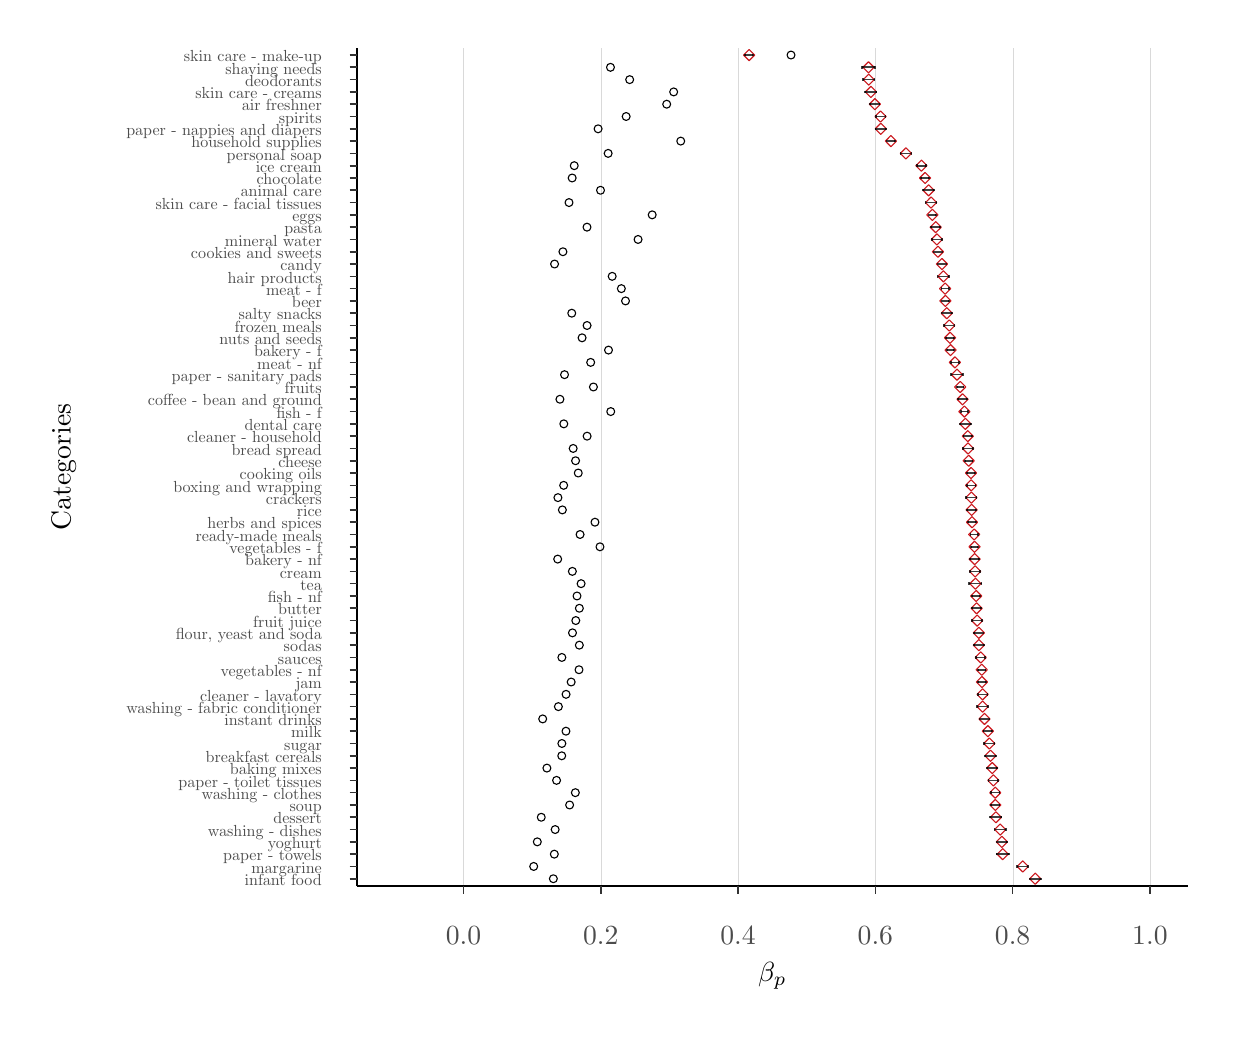
\begin{tikzpicture}[x=1pt,y=1pt]
\definecolor{fillColor}{RGB}{255,255,255}
\path[use as bounding box,fill=fillColor,fill opacity=0.00] (0,0) rectangle (433.62,361.35);
\begin{scope}
\path[clip] (  0.00,  0.00) rectangle (433.62,361.35);
\definecolor{drawColor}{RGB}{255,255,255}
\definecolor{fillColor}{RGB}{255,255,255}

\path[draw=drawColor,line width= 0.6pt,line join=round,line cap=round,fill=fillColor] (  0.00,  0.00) rectangle (433.62,361.35);
\end{scope}
\begin{scope}
\path[clip] (119.04, 51.15) rectangle (419.17,354.12);
\definecolor{drawColor}{RGB}{255,255,255}

\path[draw=drawColor,line width= 0.3pt,line join=round] (132.68, 51.15) --
	(132.68,354.12);

\path[draw=drawColor,line width= 0.3pt,line join=round] (182.29, 51.15) --
	(182.29,354.12);

\path[draw=drawColor,line width= 0.3pt,line join=round] (231.90, 51.15) --
	(231.90,354.12);

\path[draw=drawColor,line width= 0.3pt,line join=round] (281.51, 51.15) --
	(281.51,354.12);

\path[draw=drawColor,line width= 0.3pt,line join=round] (331.11, 51.15) --
	(331.11,354.12);

\path[draw=drawColor,line width= 0.3pt,line join=round] (380.72, 51.15) --
	(380.72,354.12);
\definecolor{drawColor}{gray}{0.85}

\path[draw=drawColor,line width= 0.1pt,line join=round] (157.49, 51.15) --
	(157.49,354.12);

\path[draw=drawColor,line width= 0.1pt,line join=round] (207.09, 51.15) --
	(207.09,354.12);

\path[draw=drawColor,line width= 0.1pt,line join=round] (256.70, 51.15) --
	(256.70,354.12);

\path[draw=drawColor,line width= 0.1pt,line join=round] (306.31, 51.15) --
	(306.31,354.12);

\path[draw=drawColor,line width= 0.1pt,line join=round] (355.92, 51.15) --
	(355.92,354.12);

\path[draw=drawColor,line width= 0.1pt,line join=round] (405.52, 51.15) --
	(405.52,354.12);
\definecolor{drawColor}{RGB}{0,0,0}

\path[draw=drawColor,line width= 0.4pt,line join=round,line cap=round] (230.91,333.69) circle (  1.43);

\path[draw=drawColor,line width= 0.4pt,line join=round,line cap=round] (206.99,302.59) circle (  1.43);

\path[draw=drawColor,line width= 0.4pt,line join=round,line cap=round] (209.88,244.84) circle (  1.43);

\path[draw=drawColor,line width= 0.4pt,line join=round,line cap=round] (191.52,169.32) circle (  1.43);

\path[draw=drawColor,line width= 0.4pt,line join=round,line cap=round] (187.62, 93.80) circle (  1.43);

\path[draw=drawColor,line width= 0.4pt,line join=round,line cap=round] (216.03,262.61) circle (  1.43);

\path[draw=drawColor,line width= 0.4pt,line join=round,line cap=round] (193.68,195.97) circle (  1.43);

\path[draw=drawColor,line width= 0.4pt,line join=round,line cap=round] (197.11,209.30) circle (  1.43);

\path[draw=drawColor,line width= 0.4pt,line join=round,line cap=round] (192.98, 98.24) circle (  1.43);

\path[draw=drawColor,line width= 0.4pt,line join=round,line cap=round] (199.35,151.55) circle (  1.43);

\path[draw=drawColor,line width= 0.4pt,line join=round,line cap=round] (190.39,275.94) circle (  1.43);

\path[draw=drawColor,line width= 0.4pt,line join=round,line cap=round] (197.98,204.86) circle (  1.43);

\path[draw=drawColor,line width= 0.4pt,line join=round,line cap=round] (196.75,307.03) circle (  1.43);

\path[draw=drawColor,line width= 0.4pt,line join=round,line cap=round] (202.15,213.74) circle (  1.43);

\path[draw=drawColor,line width= 0.4pt,line join=round,line cap=round] (194.54,120.45) circle (  1.43);

\path[draw=drawColor,line width= 0.4pt,line join=round,line cap=round] (192.33,227.07) circle (  1.43);

\path[draw=drawColor,line width= 0.4pt,line join=round,line cap=round] (193.41,280.38) circle (  1.43);

\path[draw=drawColor,line width= 0.4pt,line join=round,line cap=round] (198.95,200.42) circle (  1.43);

\path[draw=drawColor,line width= 0.4pt,line join=round,line cap=round] (191.61,191.53) circle (  1.43);

\path[draw=drawColor,line width= 0.4pt,line join=round,line cap=round] (196.82,164.88) circle (  1.43);

\path[draw=drawColor,line width= 0.4pt,line join=round,line cap=round] (193.73,218.19) circle (  1.43);

\path[draw=drawColor,line width= 0.4pt,line join=round,line cap=round] (217.53,342.57) circle (  1.43);

\path[draw=drawColor,line width= 0.4pt,line join=round,line cap=round] (185.58, 76.03) circle (  1.43);

\path[draw=drawColor,line width= 0.4pt,line join=round,line cap=round] (225.67,293.71) circle (  1.43);

\path[draw=drawColor,line width= 0.4pt,line join=round,line cap=round] (210.69,222.63) circle (  1.43);

\path[draw=drawColor,line width= 0.4pt,line join=round,line cap=round] (198.50,155.99) circle (  1.43);

\path[draw=drawColor,line width= 0.4pt,line join=round,line cap=round] (196.87,142.67) circle (  1.43);

\path[draw=drawColor,line width= 0.4pt,line join=round,line cap=round] (202.13,253.73) circle (  1.43);

\path[draw=drawColor,line width= 0.4pt,line join=round,line cap=round] (198.06,147.11) circle (  1.43);

\path[draw=drawColor,line width= 0.4pt,line join=round,line cap=round] (204.43,231.51) circle (  1.43);

\path[draw=drawColor,line width= 0.4pt,line join=round,line cap=round] (211.21,271.49) circle (  1.43);

\path[draw=drawColor,line width= 0.4pt,line join=round,line cap=round] (204.99,182.65) circle (  1.43);

\path[draw=drawColor,line width= 0.4pt,line join=round,line cap=round] (235.98,320.36) circle (  1.43);

\path[draw=drawColor,line width= 0.4pt,line join=round,line cap=round] (197.50,311.48) circle (  1.43);

\path[draw=drawColor,line width= 0.4pt,line join=round,line cap=round] (189.95, 53.82) circle (  1.43);

\path[draw=drawColor,line width= 0.4pt,line join=round,line cap=round] (186.10,111.57) circle (  1.43);

\path[draw=drawColor,line width= 0.4pt,line join=round,line cap=round] (196.39,124.90) circle (  1.43);

\path[draw=drawColor,line width= 0.4pt,line join=round,line cap=round] (182.85, 58.26) circle (  1.43);

\path[draw=drawColor,line width= 0.4pt,line join=round,line cap=round] (214.52,267.05) circle (  1.43);

\path[draw=drawColor,line width= 0.4pt,line join=round,line cap=round] (203.44,240.40) circle (  1.43);

\path[draw=drawColor,line width= 0.4pt,line join=round,line cap=round] (194.51,107.13) circle (  1.43);

\path[draw=drawColor,line width= 0.4pt,line join=round,line cap=round] (220.56,284.82) circle (  1.43);

\path[draw=drawColor,line width= 0.4pt,line join=round,line cap=round] (200.33,249.28) circle (  1.43);

\path[draw=drawColor,line width= 0.4pt,line join=round,line cap=round] (206.12,324.80) circle (  1.43);

\path[draw=drawColor,line width= 0.4pt,line join=round,line cap=round] (193.99,235.96) circle (  1.43);

\path[draw=drawColor,line width= 0.4pt,line join=round,line cap=round] (191.11, 89.36) circle (  1.43);

\path[draw=drawColor,line width= 0.4pt,line join=round,line cap=round] (190.30, 62.70) circle (  1.43);

\path[draw=drawColor,line width= 0.4pt,line join=round,line cap=round] (202.11,289.26) circle (  1.43);

\path[draw=drawColor,line width= 0.4pt,line join=round,line cap=round] (209.75,315.92) circle (  1.43);

\path[draw=drawColor,line width= 0.4pt,line join=round,line cap=round] (199.60,178.21) circle (  1.43);

\path[draw=drawColor,line width= 0.4pt,line join=round,line cap=round] (193.21,187.09) circle (  1.43);

\path[draw=drawColor,line width= 0.4pt,line join=round,line cap=round] (196.60,258.17) circle (  1.43);

\path[draw=drawColor,line width= 0.4pt,line join=round,line cap=round] (193.03,133.78) circle (  1.43);

\path[draw=drawColor,line width= 0.4pt,line join=round,line cap=round] (210.59,347.02) circle (  1.43);

\path[draw=drawColor,line width= 0.4pt,line join=round,line cap=round] (233.43,338.13) circle (  1.43);

\path[draw=drawColor,line width= 0.4pt,line join=round,line cap=round] (195.61,298.15) circle (  1.43);

\path[draw=drawColor,line width= 0.4pt,line join=round,line cap=round] (275.83,351.46) circle (  1.43);

\path[draw=drawColor,line width= 0.4pt,line join=round,line cap=round] (199.34,138.22) circle (  1.43);

\path[draw=drawColor,line width= 0.4pt,line join=round,line cap=round] (195.83, 80.47) circle (  1.43);

\path[draw=drawColor,line width= 0.4pt,line join=round,line cap=round] (216.26,329.25) circle (  1.43);

\path[draw=drawColor,line width= 0.4pt,line join=round,line cap=round] (193.03,102.69) circle (  1.43);

\path[draw=drawColor,line width= 0.4pt,line join=round,line cap=round] (199.97,160.44) circle (  1.43);

\path[draw=drawColor,line width= 0.4pt,line join=round,line cap=round] (206.80,173.76) circle (  1.43);

\path[draw=drawColor,line width= 0.4pt,line join=round,line cap=round] (199.22,129.34) circle (  1.43);

\path[draw=drawColor,line width= 0.4pt,line join=round,line cap=round] (197.90, 84.92) circle (  1.43);

\path[draw=drawColor,line width= 0.4pt,line join=round,line cap=round] (190.60, 71.59) circle (  1.43);

\path[draw=drawColor,line width= 0.4pt,line join=round,line cap=round] (191.77,116.01) circle (  1.43);

\path[draw=drawColor,line width= 0.4pt,line join=round,line cap=round] (184.15, 67.15) circle (  1.43);
\definecolor{drawColor}{RGB}{203,24,29}

\path[draw=drawColor,line width= 0.4pt,line join=round,line cap=round] (304.12,333.69) --
	(306.13,335.71) --
	(308.15,333.69) --
	(306.13,331.67) --
	cycle;

\path[draw=drawColor,line width= 0.4pt,line join=round,line cap=round] (323.54,302.59) --
	(325.56,304.61) --
	(327.58,302.59) --
	(325.56,300.57) --
	cycle;

\path[draw=drawColor,line width= 0.4pt,line join=round,line cap=round] (331.45,244.84) --
	(333.47,246.86) --
	(335.49,244.84) --
	(333.47,242.82) --
	cycle;

\path[draw=drawColor,line width= 0.4pt,line join=round,line cap=round] (340.18,169.32) --
	(342.19,171.34) --
	(344.21,169.32) --
	(342.19,167.30) --
	cycle;

\path[draw=drawColor,line width= 0.4pt,line join=round,line cap=round] (346.53, 93.80) --
	(348.55, 95.82) --
	(350.57, 93.80) --
	(348.55, 91.78) --
	cycle;

\path[draw=drawColor,line width= 0.4pt,line join=round,line cap=round] (329.61,262.61) --
	(331.63,264.63) --
	(333.65,262.61) --
	(331.63,260.59) --
	cycle;

\path[draw=drawColor,line width= 0.4pt,line join=round,line cap=round] (338.91,195.97) --
	(340.93,197.99) --
	(342.95,195.97) --
	(340.93,193.96) --
	cycle;

\path[draw=drawColor,line width= 0.4pt,line join=round,line cap=round] (337.77,209.30) --
	(339.79,211.32) --
	(341.81,209.30) --
	(339.79,207.28) --
	cycle;

\path[draw=drawColor,line width= 0.4pt,line join=round,line cap=round] (345.89, 98.24) --
	(347.91,100.26) --
	(349.93, 98.24) --
	(347.91, 96.23) --
	cycle;

\path[draw=drawColor,line width= 0.4pt,line join=round,line cap=round] (340.89,151.55) --
	(342.90,153.57) --
	(344.92,151.55) --
	(342.90,149.53) --
	cycle;

\path[draw=drawColor,line width= 0.4pt,line join=round,line cap=round] (328.36,275.94) --
	(330.38,277.95) --
	(332.39,275.94) --
	(330.38,273.92) --
	cycle;

\path[draw=drawColor,line width= 0.4pt,line join=round,line cap=round] (338.01,204.86) --
	(340.02,206.88) --
	(342.04,204.86) --
	(340.02,202.84) --
	cycle;

\path[draw=drawColor,line width= 0.4pt,line join=round,line cap=round] (322.26,307.03) --
	(324.28,309.05) --
	(326.29,307.03) --
	(324.28,305.02) --
	cycle;

\path[draw=drawColor,line width= 0.4pt,line join=round,line cap=round] (337.69,213.74) --
	(339.70,215.76) --
	(341.72,213.74) --
	(339.70,211.73) --
	cycle;

\path[draw=drawColor,line width= 0.4pt,line join=round,line cap=round] (343.03,120.45) --
	(345.05,122.47) --
	(347.07,120.45) --
	(345.05,118.44) --
	cycle;

\path[draw=drawColor,line width= 0.4pt,line join=round,line cap=round] (335.81,227.07) --
	(337.82,229.09) --
	(339.84,227.07) --
	(337.82,225.05) --
	cycle;

\path[draw=drawColor,line width= 0.4pt,line join=round,line cap=round] (326.90,280.38) --
	(328.92,282.40) --
	(330.93,280.38) --
	(328.92,278.36) --
	cycle;

\path[draw=drawColor,line width= 0.4pt,line join=round,line cap=round] (338.86,200.42) --
	(340.87,202.43) --
	(342.89,200.42) --
	(340.87,198.40) --
	cycle;

\path[draw=drawColor,line width= 0.4pt,line join=round,line cap=round] (338.98,191.53) --
	(340.99,193.55) --
	(343.01,191.53) --
	(340.99,189.51) --
	cycle;

\path[draw=drawColor,line width= 0.4pt,line join=round,line cap=round] (340.35,164.88) --
	(342.37,166.90) --
	(344.39,164.88) --
	(342.37,162.86) --
	cycle;

\path[draw=drawColor,line width= 0.4pt,line join=round,line cap=round] (336.80,218.19) --
	(338.82,220.20) --
	(340.83,218.19) --
	(338.82,216.17) --
	cycle;

\path[draw=drawColor,line width= 0.4pt,line join=round,line cap=round] (301.90,342.57) --
	(303.92,344.59) --
	(305.93,342.57) --
	(303.92,340.56) --
	cycle;

\path[draw=drawColor,line width= 0.4pt,line join=round,line cap=round] (347.84, 76.03) --
	(349.86, 78.05) --
	(351.88, 76.03) --
	(349.86, 74.01) --
	cycle;

\path[draw=drawColor,line width= 0.4pt,line join=round,line cap=round] (324.89,293.71) --
	(326.90,295.72) --
	(328.92,293.71) --
	(326.90,291.69) --
	cycle;

\path[draw=drawColor,line width= 0.4pt,line join=round,line cap=round] (336.46,222.63) --
	(338.47,224.65) --
	(340.49,222.63) --
	(338.47,220.61) --
	cycle;

\path[draw=drawColor,line width= 0.4pt,line join=round,line cap=round] (340.71,155.99) --
	(342.73,158.01) --
	(344.75,155.99) --
	(342.73,153.98) --
	cycle;

\path[draw=drawColor,line width= 0.4pt,line join=round,line cap=round] (341.68,142.67) --
	(343.70,144.68) --
	(345.72,142.67) --
	(343.70,140.65) --
	cycle;

\path[draw=drawColor,line width= 0.4pt,line join=round,line cap=round] (331.00,253.73) --
	(333.01,255.74) --
	(335.03,253.73) --
	(333.01,251.71) --
	cycle;

\path[draw=drawColor,line width= 0.4pt,line join=round,line cap=round] (341.07,147.11) --
	(343.09,149.13) --
	(345.11,147.11) --
	(343.09,145.09) --
	cycle;

\path[draw=drawColor,line width= 0.4pt,line join=round,line cap=round] (334.94,231.51) --
	(336.96,233.53) --
	(338.98,231.51) --
	(336.96,229.50) --
	cycle;

\path[draw=drawColor,line width= 0.4pt,line join=round,line cap=round] (328.88,271.49) --
	(330.90,273.51) --
	(332.91,271.49) --
	(330.90,269.48) --
	cycle;

\path[draw=drawColor,line width= 0.4pt,line join=round,line cap=round] (339.22,182.65) --
	(341.23,184.67) --
	(343.25,182.65) --
	(341.23,180.63) --
	cycle;

\path[draw=drawColor,line width= 0.4pt,line join=round,line cap=round] (309.93,320.36) --
	(311.94,322.38) --
	(313.96,320.36) --
	(311.94,318.34) --
	cycle;

\path[draw=drawColor,line width= 0.4pt,line join=round,line cap=round] (320.94,311.48) --
	(322.96,313.49) --
	(324.97,311.48) --
	(322.96,309.46) --
	cycle;

\path[draw=drawColor,line width= 0.4pt,line join=round,line cap=round] (362.04, 53.82) --
	(364.06, 55.84) --
	(366.07, 53.82) --
	(364.06, 51.80) --
	cycle;

\path[draw=drawColor,line width= 0.4pt,line join=round,line cap=round] (343.72,111.57) --
	(345.74,113.59) --
	(347.76,111.57) --
	(345.74,109.55) --
	cycle;

\path[draw=drawColor,line width= 0.4pt,line join=round,line cap=round] (342.81,124.90) --
	(344.83,126.91) --
	(346.85,124.90) --
	(344.83,122.88) --
	cycle;

\path[draw=drawColor,line width= 0.4pt,line join=round,line cap=round] (357.55, 58.26) --
	(359.57, 60.28) --
	(361.59, 58.26) --
	(359.57, 56.24) --
	cycle;

\path[draw=drawColor,line width= 0.4pt,line join=round,line cap=round] (329.49,267.05) --
	(331.51,269.07) --
	(333.53,267.05) --
	(331.51,265.04) --
	cycle;

\path[draw=drawColor,line width= 0.4pt,line join=round,line cap=round] (333.05,240.40) --
	(335.07,242.42) --
	(337.08,240.40) --
	(335.07,238.38) --
	cycle;

\path[draw=drawColor,line width= 0.4pt,line join=round,line cap=round] (344.95,107.13) --
	(346.96,109.14) --
	(348.98,107.13) --
	(346.96,105.11) --
	cycle;

\path[draw=drawColor,line width= 0.4pt,line join=round,line cap=round] (326.53,284.82) --
	(328.55,286.84) --
	(330.57,284.82) --
	(328.55,282.80) --
	cycle;

\path[draw=drawColor,line width= 0.4pt,line join=round,line cap=round] (331.27,249.28) --
	(333.29,251.30) --
	(335.31,249.28) --
	(333.29,247.27) --
	cycle;

\path[draw=drawColor,line width= 0.4pt,line join=round,line cap=round] (306.25,324.80) --
	(308.27,326.82) --
	(310.29,324.80) --
	(308.27,322.79) --
	cycle;

\path[draw=drawColor,line width= 0.4pt,line join=round,line cap=round] (333.78,235.96) --
	(335.80,237.97) --
	(337.81,235.96) --
	(335.80,233.94) --
	cycle;

\path[draw=drawColor,line width= 0.4pt,line join=round,line cap=round] (346.94, 89.36) --
	(348.96, 91.38) --
	(350.98, 89.36) --
	(348.96, 87.34) --
	cycle;

\path[draw=drawColor,line width= 0.4pt,line join=round,line cap=round] (350.31, 62.70) --
	(352.33, 64.72) --
	(354.35, 62.70) --
	(352.33, 60.69) --
	cycle;

\path[draw=drawColor,line width= 0.4pt,line join=round,line cap=round] (326.10,289.26) --
	(328.12,291.28) --
	(330.14,289.26) --
	(328.12,287.25) --
	cycle;

\path[draw=drawColor,line width= 0.4pt,line join=round,line cap=round] (315.34,315.92) --
	(317.35,317.94) --
	(319.37,315.92) --
	(317.35,313.90) --
	cycle;

\path[draw=drawColor,line width= 0.4pt,line join=round,line cap=round] (339.99,178.21) --
	(342.00,180.22) --
	(344.02,178.21) --
	(342.00,176.19) --
	cycle;

\path[draw=drawColor,line width= 0.4pt,line join=round,line cap=round] (339.07,187.09) --
	(341.09,189.11) --
	(343.11,187.09) --
	(341.09,185.07) --
	cycle;

\path[draw=drawColor,line width= 0.4pt,line join=round,line cap=round] (330.10,258.17) --
	(332.12,260.19) --
	(334.13,258.17) --
	(332.12,256.15) --
	cycle;

\path[draw=drawColor,line width= 0.4pt,line join=round,line cap=round] (342.38,133.78) --
	(344.40,135.80) --
	(346.41,133.78) --
	(344.40,131.76) --
	cycle;

\path[draw=drawColor,line width= 0.4pt,line join=round,line cap=round] (301.81,347.02) --
	(303.83,349.03) --
	(305.84,347.02) --
	(303.83,345.00) --
	cycle;

\path[draw=drawColor,line width= 0.4pt,line join=round,line cap=round] (302.68,338.13) --
	(304.70,340.15) --
	(306.71,338.13) --
	(304.70,336.11) --
	cycle;

\path[draw=drawColor,line width= 0.4pt,line join=round,line cap=round] (324.42,298.15) --
	(326.43,300.17) --
	(328.45,298.15) --
	(326.43,296.13) --
	cycle;

\path[draw=drawColor,line width= 0.4pt,line join=round,line cap=round] (258.68,351.46) --
	(260.69,353.48) --
	(262.71,351.46) --
	(260.69,349.44) --
	cycle;

\path[draw=drawColor,line width= 0.4pt,line join=round,line cap=round] (341.69,138.22) --
	(343.71,140.24) --
	(345.73,138.22) --
	(343.71,136.21) --
	cycle;

\path[draw=drawColor,line width= 0.4pt,line join=round,line cap=round] (347.65, 80.47) --
	(349.66, 82.49) --
	(351.68, 80.47) --
	(349.66, 78.46) --
	cycle;

\path[draw=drawColor,line width= 0.4pt,line join=round,line cap=round] (306.16,329.25) --
	(308.18,331.26) --
	(310.20,329.25) --
	(308.18,327.23) --
	cycle;

\path[draw=drawColor,line width= 0.4pt,line join=round,line cap=round] (345.47,102.69) --
	(347.49,104.70) --
	(349.50,102.69) --
	(347.49,100.67) --
	cycle;

\path[draw=drawColor,line width= 0.4pt,line join=round,line cap=round] (340.45,160.44) --
	(342.47,162.45) --
	(344.48,160.44) --
	(342.47,158.42) --
	cycle;

\path[draw=drawColor,line width= 0.4pt,line join=round,line cap=round] (340.13,173.76) --
	(342.15,175.78) --
	(344.17,173.76) --
	(342.15,171.75) --
	cycle;

\path[draw=drawColor,line width= 0.4pt,line join=round,line cap=round] (342.72,129.34) --
	(344.74,131.36) --
	(346.76,129.34) --
	(344.74,127.32) --
	cycle;

\path[draw=drawColor,line width= 0.4pt,line join=round,line cap=round] (347.61, 84.92) --
	(349.63, 86.93) --
	(351.64, 84.92) --
	(349.63, 82.90) --
	cycle;

\path[draw=drawColor,line width= 0.4pt,line join=round,line cap=round] (349.39, 71.59) --
	(351.41, 73.61) --
	(353.42, 71.59) --
	(351.41, 69.57) --
	cycle;

\path[draw=drawColor,line width= 0.4pt,line join=round,line cap=round] (343.07,116.01) --
	(345.08,118.03) --
	(347.10,116.01) --
	(345.08,113.99) --
	cycle;

\path[draw=drawColor,line width= 0.4pt,line join=round,line cap=round] (350.01, 67.15) --
	(352.03, 69.16) --
	(354.05, 67.15) --
	(352.03, 65.13) --
	cycle;
\definecolor{drawColor}{RGB}{0,0,0}

\path[draw=drawColor,draw opacity=0.75,line width= 0.6pt,line join=round] (307.83,333.24) --
	(307.83,334.13);

\path[draw=drawColor,draw opacity=0.75,line width= 0.6pt,line join=round] (307.83,333.69) --
	(304.44,333.69);

\path[draw=drawColor,draw opacity=0.75,line width= 0.6pt,line join=round] (304.44,333.24) --
	(304.44,334.13);

\path[draw=drawColor,draw opacity=0.75,line width= 0.6pt,line join=round] (327.51,302.15) --
	(327.51,303.04);

\path[draw=drawColor,draw opacity=0.75,line width= 0.6pt,line join=round] (327.51,302.59) --
	(323.61,302.59);

\path[draw=drawColor,draw opacity=0.75,line width= 0.6pt,line join=round] (323.61,302.15) --
	(323.61,303.04);

\path[draw=drawColor,draw opacity=0.75,line width= 0.6pt,line join=round] (334.71,244.40) --
	(334.71,245.29);

\path[draw=drawColor,draw opacity=0.75,line width= 0.6pt,line join=round] (334.71,244.84) --
	(332.23,244.84);

\path[draw=drawColor,draw opacity=0.75,line width= 0.6pt,line join=round] (332.23,244.40) --
	(332.23,245.29);

\path[draw=drawColor,draw opacity=0.75,line width= 0.6pt,line join=round] (343.80,168.88) --
	(343.80,169.76);

\path[draw=drawColor,draw opacity=0.75,line width= 0.6pt,line join=round] (343.80,169.32) --
	(340.59,169.32);

\path[draw=drawColor,draw opacity=0.75,line width= 0.6pt,line join=round] (340.59,168.88) --
	(340.59,169.76);

\path[draw=drawColor,draw opacity=0.75,line width= 0.6pt,line join=round] (350.38, 93.36) --
	(350.38, 94.24);

\path[draw=drawColor,draw opacity=0.75,line width= 0.6pt,line join=round] (350.38, 93.80) --
	(346.72, 93.80);

\path[draw=drawColor,draw opacity=0.75,line width= 0.6pt,line join=round] (346.72, 93.36) --
	(346.72, 94.24);

\path[draw=drawColor,draw opacity=0.75,line width= 0.6pt,line join=round] (333.03,262.17) --
	(333.03,263.05);

\path[draw=drawColor,draw opacity=0.75,line width= 0.6pt,line join=round] (333.03,262.61) --
	(330.23,262.61);

\path[draw=drawColor,draw opacity=0.75,line width= 0.6pt,line join=round] (330.23,262.17) --
	(330.23,263.05);

\path[draw=drawColor,draw opacity=0.75,line width= 0.6pt,line join=round] (342.53,195.53) --
	(342.53,196.42);

\path[draw=drawColor,draw opacity=0.75,line width= 0.6pt,line join=round] (342.53,195.97) --
	(339.33,195.97);

\path[draw=drawColor,draw opacity=0.75,line width= 0.6pt,line join=round] (339.33,195.53) --
	(339.33,196.42);

\path[draw=drawColor,draw opacity=0.75,line width= 0.6pt,line join=round] (341.57,208.86) --
	(341.57,209.75);

\path[draw=drawColor,draw opacity=0.75,line width= 0.6pt,line join=round] (341.57,209.30) --
	(338.02,209.30);

\path[draw=drawColor,draw opacity=0.75,line width= 0.6pt,line join=round] (338.02,208.86) --
	(338.02,209.75);

\path[draw=drawColor,draw opacity=0.75,line width= 0.6pt,line join=round] (349.82, 97.80) --
	(349.82, 98.69);

\path[draw=drawColor,draw opacity=0.75,line width= 0.6pt,line join=round] (349.82, 98.24) --
	(346.00, 98.24);

\path[draw=drawColor,draw opacity=0.75,line width= 0.6pt,line join=round] (346.00, 97.80) --
	(346.00, 98.69);

\path[draw=drawColor,draw opacity=0.75,line width= 0.6pt,line join=round] (344.52,151.11) --
	(344.52,152.00);

\path[draw=drawColor,draw opacity=0.75,line width= 0.6pt,line join=round] (344.52,151.55) --
	(341.28,151.55);

\path[draw=drawColor,draw opacity=0.75,line width= 0.6pt,line join=round] (341.28,151.11) --
	(341.28,152.00);

\path[draw=drawColor,draw opacity=0.75,line width= 0.6pt,line join=round] (331.97,275.49) --
	(331.97,276.38);

\path[draw=drawColor,draw opacity=0.75,line width= 0.6pt,line join=round] (331.97,275.94) --
	(328.78,275.94);

\path[draw=drawColor,draw opacity=0.75,line width= 0.6pt,line join=round] (328.78,275.49) --
	(328.78,276.38);

\path[draw=drawColor,draw opacity=0.75,line width= 0.6pt,line join=round] (341.44,204.42) --
	(341.44,205.30);

\path[draw=drawColor,draw opacity=0.75,line width= 0.6pt,line join=round] (341.44,204.86) --
	(338.61,204.86);

\path[draw=drawColor,draw opacity=0.75,line width= 0.6pt,line join=round] (338.61,204.42) --
	(338.61,205.30);

\path[draw=drawColor,draw opacity=0.75,line width= 0.6pt,line join=round] (325.76,306.59) --
	(325.76,307.48);

\path[draw=drawColor,draw opacity=0.75,line width= 0.6pt,line join=round] (325.76,307.03) --
	(322.79,307.03);

\path[draw=drawColor,draw opacity=0.75,line width= 0.6pt,line join=round] (322.79,306.59) --
	(322.79,307.48);

\path[draw=drawColor,draw opacity=0.75,line width= 0.6pt,line join=round] (341.30,213.30) --
	(341.30,214.19);

\path[draw=drawColor,draw opacity=0.75,line width= 0.6pt,line join=round] (341.30,213.74) --
	(338.10,213.74);

\path[draw=drawColor,draw opacity=0.75,line width= 0.6pt,line join=round] (338.10,213.30) --
	(338.10,214.19);

\path[draw=drawColor,draw opacity=0.75,line width= 0.6pt,line join=round] (346.81,120.01) --
	(346.81,120.90);

\path[draw=drawColor,draw opacity=0.75,line width= 0.6pt,line join=round] (346.81,120.45) --
	(343.29,120.45);

\path[draw=drawColor,draw opacity=0.75,line width= 0.6pt,line join=round] (343.29,120.01) --
	(343.29,120.90);

\path[draw=drawColor,draw opacity=0.75,line width= 0.6pt,line join=round] (339.42,226.63) --
	(339.42,227.52);

\path[draw=drawColor,draw opacity=0.75,line width= 0.6pt,line join=round] (339.42,227.07) --
	(336.23,227.07);

\path[draw=drawColor,draw opacity=0.75,line width= 0.6pt,line join=round] (336.23,226.63) --
	(336.23,227.52);

\path[draw=drawColor,draw opacity=0.75,line width= 0.6pt,line join=round] (330.52,279.94) --
	(330.52,280.82);

\path[draw=drawColor,draw opacity=0.75,line width= 0.6pt,line join=round] (330.52,280.38) --
	(327.32,280.38);

\path[draw=drawColor,draw opacity=0.75,line width= 0.6pt,line join=round] (327.32,279.94) --
	(327.32,280.82);

\path[draw=drawColor,draw opacity=0.75,line width= 0.6pt,line join=round] (342.25,199.97) --
	(342.25,200.86);

\path[draw=drawColor,draw opacity=0.75,line width= 0.6pt,line join=round] (342.25,200.42) --
	(339.49,200.42);

\path[draw=drawColor,draw opacity=0.75,line width= 0.6pt,line join=round] (339.49,199.97) --
	(339.49,200.86);

\path[draw=drawColor,draw opacity=0.75,line width= 0.6pt,line join=round] (342.89,191.09) --
	(342.89,191.98);

\path[draw=drawColor,draw opacity=0.75,line width= 0.6pt,line join=round] (342.89,191.53) --
	(339.10,191.53);

\path[draw=drawColor,draw opacity=0.75,line width= 0.6pt,line join=round] (339.10,191.09) --
	(339.10,191.98);

\path[draw=drawColor,draw opacity=0.75,line width= 0.6pt,line join=round] (344.16,164.43) --
	(344.16,165.32);

\path[draw=drawColor,draw opacity=0.75,line width= 0.6pt,line join=round] (344.16,164.88) --
	(340.58,164.88);

\path[draw=drawColor,draw opacity=0.75,line width= 0.6pt,line join=round] (340.58,164.43) --
	(340.58,165.32);

\path[draw=drawColor,draw opacity=0.75,line width= 0.6pt,line join=round] (340.84,217.74) --
	(340.84,218.63);

\path[draw=drawColor,draw opacity=0.75,line width= 0.6pt,line join=round] (340.84,218.19) --
	(336.79,218.19);

\path[draw=drawColor,draw opacity=0.75,line width= 0.6pt,line join=round] (336.79,217.74) --
	(336.79,218.63);

\path[draw=drawColor,draw opacity=0.75,line width= 0.6pt,line join=round] (306.00,342.13) --
	(306.00,343.02);

\path[draw=drawColor,draw opacity=0.75,line width= 0.6pt,line join=round] (306.00,342.57) --
	(301.83,342.57);

\path[draw=drawColor,draw opacity=0.75,line width= 0.6pt,line join=round] (301.83,342.13) --
	(301.83,343.02);

\path[draw=drawColor,draw opacity=0.75,line width= 0.6pt,line join=round] (351.93, 75.59) --
	(351.93, 76.48);

\path[draw=drawColor,draw opacity=0.75,line width= 0.6pt,line join=round] (351.93, 76.03) --
	(347.79, 76.03);

\path[draw=drawColor,draw opacity=0.75,line width= 0.6pt,line join=round] (347.79, 75.59) --
	(347.79, 76.48);

\path[draw=drawColor,draw opacity=0.75,line width= 0.6pt,line join=round] (328.24,293.26) --
	(328.24,294.15);

\path[draw=drawColor,draw opacity=0.75,line width= 0.6pt,line join=round] (328.24,293.71) --
	(325.57,293.71);

\path[draw=drawColor,draw opacity=0.75,line width= 0.6pt,line join=round] (325.57,293.26) --
	(325.57,294.15);

\path[draw=drawColor,draw opacity=0.75,line width= 0.6pt,line join=round] (339.69,222.18) --
	(339.69,223.07);

\path[draw=drawColor,draw opacity=0.75,line width= 0.6pt,line join=round] (339.69,222.63) --
	(337.26,222.63);

\path[draw=drawColor,draw opacity=0.75,line width= 0.6pt,line join=round] (337.26,222.18) --
	(337.26,223.07);

\path[draw=drawColor,draw opacity=0.75,line width= 0.6pt,line join=round] (344.20,155.55) --
	(344.20,156.44);

\path[draw=drawColor,draw opacity=0.75,line width= 0.6pt,line join=round] (344.20,155.99) --
	(341.26,155.99);

\path[draw=drawColor,draw opacity=0.75,line width= 0.6pt,line join=round] (341.26,155.55) --
	(341.26,156.44);

\path[draw=drawColor,draw opacity=0.75,line width= 0.6pt,line join=round] (345.36,142.22) --
	(345.36,143.11);

\path[draw=drawColor,draw opacity=0.75,line width= 0.6pt,line join=round] (345.36,142.67) --
	(342.03,142.67);

\path[draw=drawColor,draw opacity=0.75,line width= 0.6pt,line join=round] (342.03,142.22) --
	(342.03,143.11);

\path[draw=drawColor,draw opacity=0.75,line width= 0.6pt,line join=round] (334.90,253.28) --
	(334.90,254.17);

\path[draw=drawColor,draw opacity=0.75,line width= 0.6pt,line join=round] (334.90,253.73) --
	(331.13,253.73);

\path[draw=drawColor,draw opacity=0.75,line width= 0.6pt,line join=round] (331.13,253.28) --
	(331.13,254.17);

\path[draw=drawColor,draw opacity=0.75,line width= 0.6pt,line join=round] (344.84,146.66) --
	(344.84,147.55);

\path[draw=drawColor,draw opacity=0.75,line width= 0.6pt,line join=round] (344.84,147.11) --
	(341.34,147.11);

\path[draw=drawColor,draw opacity=0.75,line width= 0.6pt,line join=round] (341.34,146.66) --
	(341.34,147.55);

\path[draw=drawColor,draw opacity=0.75,line width= 0.6pt,line join=round] (338.18,231.07) --
	(338.18,231.96);

\path[draw=drawColor,draw opacity=0.75,line width= 0.6pt,line join=round] (338.18,231.51) --
	(335.73,231.51);

\path[draw=drawColor,draw opacity=0.75,line width= 0.6pt,line join=round] (335.73,231.07) --
	(335.73,231.96);

\path[draw=drawColor,draw opacity=0.75,line width= 0.6pt,line join=round] (332.98,271.05) --
	(332.98,271.94);

\path[draw=drawColor,draw opacity=0.75,line width= 0.6pt,line join=round] (332.98,271.49) --
	(328.82,271.49);

\path[draw=drawColor,draw opacity=0.75,line width= 0.6pt,line join=round] (328.82,271.05) --
	(328.82,271.94);

\path[draw=drawColor,draw opacity=0.75,line width= 0.6pt,line join=round] (342.64,182.20) --
	(342.64,183.09);

\path[draw=drawColor,draw opacity=0.75,line width= 0.6pt,line join=round] (342.64,182.65) --
	(339.83,182.65);

\path[draw=drawColor,draw opacity=0.75,line width= 0.6pt,line join=round] (339.83,182.20) --
	(339.83,183.09);

\path[draw=drawColor,draw opacity=0.75,line width= 0.6pt,line join=round] (313.49,319.92) --
	(313.49,320.81);

\path[draw=drawColor,draw opacity=0.75,line width= 0.6pt,line join=round] (313.49,320.36) --
	(310.39,320.36);

\path[draw=drawColor,draw opacity=0.75,line width= 0.6pt,line join=round] (310.39,319.92) --
	(310.39,320.81);

\path[draw=drawColor,draw opacity=0.75,line width= 0.6pt,line join=round] (324.51,311.03) --
	(324.51,311.92);

\path[draw=drawColor,draw opacity=0.75,line width= 0.6pt,line join=round] (324.51,311.48) --
	(321.41,311.48);

\path[draw=drawColor,draw opacity=0.75,line width= 0.6pt,line join=round] (321.41,311.03) --
	(321.41,311.92);

\path[draw=drawColor,draw opacity=0.75,line width= 0.6pt,line join=round] (366.08, 53.37) --
	(366.08, 54.26);

\path[draw=drawColor,draw opacity=0.75,line width= 0.6pt,line join=round] (366.08, 53.82) --
	(362.03, 53.82);

\path[draw=drawColor,draw opacity=0.75,line width= 0.6pt,line join=round] (362.03, 53.37) --
	(362.03, 54.26);

\path[draw=drawColor,draw opacity=0.75,line width= 0.6pt,line join=round] (347.50,111.13) --
	(347.50,112.01);

\path[draw=drawColor,draw opacity=0.75,line width= 0.6pt,line join=round] (347.50,111.57) --
	(343.99,111.57);

\path[draw=drawColor,draw opacity=0.75,line width= 0.6pt,line join=round] (343.99,111.13) --
	(343.99,112.01);

\path[draw=drawColor,draw opacity=0.75,line width= 0.6pt,line join=round] (346.38,124.45) --
	(346.38,125.34);

\path[draw=drawColor,draw opacity=0.75,line width= 0.6pt,line join=round] (346.38,124.90) --
	(343.28,124.90);

\path[draw=drawColor,draw opacity=0.75,line width= 0.6pt,line join=round] (343.28,124.45) --
	(343.28,125.34);

\path[draw=drawColor,draw opacity=0.75,line width= 0.6pt,line join=round] (361.57, 57.82) --
	(361.57, 58.71);

\path[draw=drawColor,draw opacity=0.75,line width= 0.6pt,line join=round] (361.57, 58.26) --
	(357.56, 58.26);

\path[draw=drawColor,draw opacity=0.75,line width= 0.6pt,line join=round] (357.56, 57.82) --
	(357.56, 58.71);

\path[draw=drawColor,draw opacity=0.75,line width= 0.6pt,line join=round] (332.84,266.61) --
	(332.84,267.50);

\path[draw=drawColor,draw opacity=0.75,line width= 0.6pt,line join=round] (332.84,267.05) --
	(330.18,267.05);

\path[draw=drawColor,draw opacity=0.75,line width= 0.6pt,line join=round] (330.18,266.61) --
	(330.18,267.50);

\path[draw=drawColor,draw opacity=0.75,line width= 0.6pt,line join=round] (336.47,239.95) --
	(336.47,240.84);

\path[draw=drawColor,draw opacity=0.75,line width= 0.6pt,line join=round] (336.47,240.40) --
	(333.66,240.40);

\path[draw=drawColor,draw opacity=0.75,line width= 0.6pt,line join=round] (333.66,239.95) --
	(333.66,240.84);

\path[draw=drawColor,draw opacity=0.75,line width= 0.6pt,line join=round] (348.57,106.68) --
	(348.57,107.57);

\path[draw=drawColor,draw opacity=0.75,line width= 0.6pt,line join=round] (348.57,107.13) --
	(345.35,107.13);

\path[draw=drawColor,draw opacity=0.75,line width= 0.6pt,line join=round] (345.35,106.68) --
	(345.35,107.57);

\path[draw=drawColor,draw opacity=0.75,line width= 0.6pt,line join=round] (330.37,284.38) --
	(330.37,285.27);

\path[draw=drawColor,draw opacity=0.75,line width= 0.6pt,line join=round] (330.37,284.82) --
	(326.72,284.82);

\path[draw=drawColor,draw opacity=0.75,line width= 0.6pt,line join=round] (326.72,284.38) --
	(326.72,285.27);

\path[draw=drawColor,draw opacity=0.75,line width= 0.6pt,line join=round] (334.67,248.84) --
	(334.67,249.73);

\path[draw=drawColor,draw opacity=0.75,line width= 0.6pt,line join=round] (334.67,249.28) --
	(331.91,249.28);

\path[draw=drawColor,draw opacity=0.75,line width= 0.6pt,line join=round] (331.91,248.84) --
	(331.91,249.73);

\path[draw=drawColor,draw opacity=0.75,line width= 0.6pt,line join=round] (310.20,324.36) --
	(310.20,325.25);

\path[draw=drawColor,draw opacity=0.75,line width= 0.6pt,line join=round] (310.20,324.80) --
	(306.34,324.80);

\path[draw=drawColor,draw opacity=0.75,line width= 0.6pt,line join=round] (306.34,324.36) --
	(306.34,325.25);

\path[draw=drawColor,draw opacity=0.75,line width= 0.6pt,line join=round] (338.01,235.51) --
	(338.01,236.40);

\path[draw=drawColor,draw opacity=0.75,line width= 0.6pt,line join=round] (338.01,235.96) --
	(333.58,235.96);

\path[draw=drawColor,draw opacity=0.75,line width= 0.6pt,line join=round] (333.58,235.51) --
	(333.58,236.40);

\path[draw=drawColor,draw opacity=0.75,line width= 0.6pt,line join=round] (350.67, 88.91) --
	(350.67, 89.80);

\path[draw=drawColor,draw opacity=0.75,line width= 0.6pt,line join=round] (350.67, 89.36) --
	(347.25, 89.36);

\path[draw=drawColor,draw opacity=0.75,line width= 0.6pt,line join=round] (347.25, 88.91) --
	(347.25, 89.80);

\path[draw=drawColor,draw opacity=0.75,line width= 0.6pt,line join=round] (354.61, 62.26) --
	(354.61, 63.15);

\path[draw=drawColor,draw opacity=0.75,line width= 0.6pt,line join=round] (354.61, 62.70) --
	(350.05, 62.70);

\path[draw=drawColor,draw opacity=0.75,line width= 0.6pt,line join=round] (350.05, 62.26) --
	(350.05, 63.15);

\path[draw=drawColor,draw opacity=0.75,line width= 0.6pt,line join=round] (329.77,288.82) --
	(329.77,289.71);

\path[draw=drawColor,draw opacity=0.75,line width= 0.6pt,line join=round] (329.77,289.26) --
	(326.47,289.26);

\path[draw=drawColor,draw opacity=0.75,line width= 0.6pt,line join=round] (326.47,288.82) --
	(326.47,289.71);

\path[draw=drawColor,draw opacity=0.75,line width= 0.6pt,line join=round] (319.35,315.47) --
	(319.35,316.36);

\path[draw=drawColor,draw opacity=0.75,line width= 0.6pt,line join=round] (319.35,315.92) --
	(315.36,315.92);

\path[draw=drawColor,draw opacity=0.75,line width= 0.6pt,line join=round] (315.36,315.47) --
	(315.36,316.36);

\path[draw=drawColor,draw opacity=0.75,line width= 0.6pt,line join=round] (343.35,177.76) --
	(343.35,178.65);

\path[draw=drawColor,draw opacity=0.75,line width= 0.6pt,line join=round] (343.35,178.21) --
	(340.66,178.21);

\path[draw=drawColor,draw opacity=0.75,line width= 0.6pt,line join=round] (340.66,177.76) --
	(340.66,178.65);

\path[draw=drawColor,draw opacity=0.75,line width= 0.6pt,line join=round] (342.68,186.65) --
	(342.68,187.53);

\path[draw=drawColor,draw opacity=0.75,line width= 0.6pt,line join=round] (342.68,187.09) --
	(339.50,187.09);

\path[draw=drawColor,draw opacity=0.75,line width= 0.6pt,line join=round] (339.50,186.65) --
	(339.50,187.53);

\path[draw=drawColor,draw opacity=0.75,line width= 0.6pt,line join=round] (333.98,257.72) --
	(333.98,258.61);

\path[draw=drawColor,draw opacity=0.75,line width= 0.6pt,line join=round] (333.98,258.17) --
	(330.25,258.17);

\path[draw=drawColor,draw opacity=0.75,line width= 0.6pt,line join=round] (330.25,257.72) --
	(330.25,258.61);

\path[draw=drawColor,draw opacity=0.75,line width= 0.6pt,line join=round] (346.01,133.34) --
	(346.01,134.23);

\path[draw=drawColor,draw opacity=0.75,line width= 0.6pt,line join=round] (346.01,133.78) --
	(342.78,133.78);

\path[draw=drawColor,draw opacity=0.75,line width= 0.6pt,line join=round] (342.78,133.34) --
	(342.78,134.23);

\path[draw=drawColor,draw opacity=0.75,line width= 0.6pt,line join=round] (306.08,346.57) --
	(306.08,347.46);

\path[draw=drawColor,draw opacity=0.75,line width= 0.6pt,line join=round] (306.08,347.02) --
	(301.57,347.02);

\path[draw=drawColor,draw opacity=0.75,line width= 0.6pt,line join=round] (301.57,346.57) --
	(301.57,347.46);

\path[draw=drawColor,draw opacity=0.75,line width= 0.6pt,line join=round] (306.76,337.69) --
	(306.76,338.57);

\path[draw=drawColor,draw opacity=0.75,line width= 0.6pt,line join=round] (306.76,338.13) --
	(302.63,338.13);

\path[draw=drawColor,draw opacity=0.75,line width= 0.6pt,line join=round] (302.63,337.69) --
	(302.63,338.57);

\path[draw=drawColor,draw opacity=0.75,line width= 0.6pt,line join=round] (328.42,297.70) --
	(328.42,298.59);

\path[draw=drawColor,draw opacity=0.75,line width= 0.6pt,line join=round] (328.42,298.15) --
	(324.44,298.15);

\path[draw=drawColor,draw opacity=0.75,line width= 0.6pt,line join=round] (324.44,297.70) --
	(324.44,298.59);

\path[draw=drawColor,draw opacity=0.75,line width= 0.6pt,line join=round] (262.20,351.01) --
	(262.20,351.90);

\path[draw=drawColor,draw opacity=0.75,line width= 0.6pt,line join=round] (262.20,351.46) --
	(259.19,351.46);

\path[draw=drawColor,draw opacity=0.75,line width= 0.6pt,line join=round] (259.19,351.01) --
	(259.19,351.90);

\path[draw=drawColor,draw opacity=0.75,line width= 0.6pt,line join=round] (345.46,137.78) --
	(345.46,138.67);

\path[draw=drawColor,draw opacity=0.75,line width= 0.6pt,line join=round] (345.46,138.22) --
	(341.96,138.22);

\path[draw=drawColor,draw opacity=0.75,line width= 0.6pt,line join=round] (341.96,137.78) --
	(341.96,138.67);

\path[draw=drawColor,draw opacity=0.75,line width= 0.6pt,line join=round] (351.22, 80.03) --
	(351.22, 80.92);

\path[draw=drawColor,draw opacity=0.75,line width= 0.6pt,line join=round] (351.22, 80.47) --
	(348.11, 80.47);

\path[draw=drawColor,draw opacity=0.75,line width= 0.6pt,line join=round] (348.11, 80.03) --
	(348.11, 80.92);

\path[draw=drawColor,draw opacity=0.75,line width= 0.6pt,line join=round] (309.91,328.80) --
	(309.91,329.69);

\path[draw=drawColor,draw opacity=0.75,line width= 0.6pt,line join=round] (309.91,329.25) --
	(306.45,329.25);

\path[draw=drawColor,draw opacity=0.75,line width= 0.6pt,line join=round] (306.45,328.80) --
	(306.45,329.69);

\path[draw=drawColor,draw opacity=0.75,line width= 0.6pt,line join=round] (349.40,102.24) --
	(349.40,103.13);

\path[draw=drawColor,draw opacity=0.75,line width= 0.6pt,line join=round] (349.40,102.69) --
	(345.57,102.69);

\path[draw=drawColor,draw opacity=0.75,line width= 0.6pt,line join=round] (345.57,102.24) --
	(345.57,103.13);

\path[draw=drawColor,draw opacity=0.75,line width= 0.6pt,line join=round] (344.69,159.99) --
	(344.69,160.88);

\path[draw=drawColor,draw opacity=0.75,line width= 0.6pt,line join=round] (344.69,160.44) --
	(340.24,160.44);

\path[draw=drawColor,draw opacity=0.75,line width= 0.6pt,line join=round] (340.24,159.99) --
	(340.24,160.88);

\path[draw=drawColor,draw opacity=0.75,line width= 0.6pt,line join=round] (343.35,173.32) --
	(343.35,174.21);

\path[draw=drawColor,draw opacity=0.75,line width= 0.6pt,line join=round] (343.35,173.76) --
	(340.95,173.76);

\path[draw=drawColor,draw opacity=0.75,line width= 0.6pt,line join=round] (340.95,173.32) --
	(340.95,174.21);

\path[draw=drawColor,draw opacity=0.75,line width= 0.6pt,line join=round] (346.11,128.90) --
	(346.11,129.78);

\path[draw=drawColor,draw opacity=0.75,line width= 0.6pt,line join=round] (346.11,129.34) --
	(343.36,129.34);

\path[draw=drawColor,draw opacity=0.75,line width= 0.6pt,line join=round] (343.36,128.90) --
	(343.36,129.78);

\path[draw=drawColor,draw opacity=0.75,line width= 0.6pt,line join=round] (351.21, 84.47) --
	(351.21, 85.36);

\path[draw=drawColor,draw opacity=0.75,line width= 0.6pt,line join=round] (351.21, 84.92) --
	(348.05, 84.92);

\path[draw=drawColor,draw opacity=0.75,line width= 0.6pt,line join=round] (348.05, 84.47) --
	(348.05, 85.36);

\path[draw=drawColor,draw opacity=0.75,line width= 0.6pt,line join=round] (353.45, 71.14) --
	(353.45, 72.03);

\path[draw=drawColor,draw opacity=0.75,line width= 0.6pt,line join=round] (353.45, 71.59) --
	(349.36, 71.59);

\path[draw=drawColor,draw opacity=0.75,line width= 0.6pt,line join=round] (349.36, 71.14) --
	(349.36, 72.03);

\path[draw=drawColor,draw opacity=0.75,line width= 0.6pt,line join=round] (347.06,115.57) --
	(347.06,116.46);

\path[draw=drawColor,draw opacity=0.75,line width= 0.6pt,line join=round] (347.06,116.01) --
	(343.11,116.01);

\path[draw=drawColor,draw opacity=0.75,line width= 0.6pt,line join=round] (343.11,115.57) --
	(343.11,116.46);

\path[draw=drawColor,draw opacity=0.75,line width= 0.6pt,line join=round] (353.92, 66.70) --
	(353.92, 67.59);

\path[draw=drawColor,draw opacity=0.75,line width= 0.6pt,line join=round] (353.92, 67.15) --
	(350.13, 67.15);

\path[draw=drawColor,draw opacity=0.75,line width= 0.6pt,line join=round] (350.13, 66.70) --
	(350.13, 67.59);
\end{scope}
\begin{scope}
\path[clip] (  0.00,  0.00) rectangle (433.62,361.35);
\definecolor{drawColor}{RGB}{0,0,0}

\path[draw=drawColor,line width= 0.6pt,line join=round] (119.04, 51.15) --
	(119.04,354.12);
\end{scope}
\begin{scope}
\path[clip] (  0.00,  0.00) rectangle (433.62,361.35);
\definecolor{drawColor}{gray}{0.30}

\node[text=drawColor,anchor=base east,inner sep=0pt, outer sep=0pt, scale=  0.58] at (106.29, 51.41) {infant food};

\node[text=drawColor,anchor=base east,inner sep=0pt, outer sep=0pt, scale=  0.58] at (106.29, 55.85) {margarine};

\node[text=drawColor,anchor=base east,inner sep=0pt, outer sep=0pt, scale=  0.58] at (106.29, 60.29) {paper - towels};

\node[text=drawColor,anchor=base east,inner sep=0pt, outer sep=0pt, scale=  0.58] at (106.29, 64.74) {yoghurt};

\node[text=drawColor,anchor=base east,inner sep=0pt, outer sep=0pt, scale=  0.58] at (106.29, 69.18) {washing - dishes};

\node[text=drawColor,anchor=base east,inner sep=0pt, outer sep=0pt, scale=  0.58] at (106.29, 73.62) {dessert};

\node[text=drawColor,anchor=base east,inner sep=0pt, outer sep=0pt, scale=  0.58] at (106.29, 78.06) {soup};

\node[text=drawColor,anchor=base east,inner sep=0pt, outer sep=0pt, scale=  0.58] at (106.29, 82.50) {washing - clothes};

\node[text=drawColor,anchor=base east,inner sep=0pt, outer sep=0pt, scale=  0.58] at (106.29, 86.95) {paper - toilet tissues};

\node[text=drawColor,anchor=base east,inner sep=0pt, outer sep=0pt, scale=  0.58] at (106.29, 91.39) {baking mixes};

\node[text=drawColor,anchor=base east,inner sep=0pt, outer sep=0pt, scale=  0.58] at (106.29, 95.83) {breakfast cereals};

\node[text=drawColor,anchor=base east,inner sep=0pt, outer sep=0pt, scale=  0.58] at (106.29,100.27) {sugar};

\node[text=drawColor,anchor=base east,inner sep=0pt, outer sep=0pt, scale=  0.58] at (106.29,104.72) {milk};

\node[text=drawColor,anchor=base east,inner sep=0pt, outer sep=0pt, scale=  0.58] at (106.29,109.16) {instant drinks};

\node[text=drawColor,anchor=base east,inner sep=0pt, outer sep=0pt, scale=  0.58] at (106.29,113.60) {washing - fabric conditioner};

\node[text=drawColor,anchor=base east,inner sep=0pt, outer sep=0pt, scale=  0.58] at (106.29,118.04) {cleaner - lavatory};

\node[text=drawColor,anchor=base east,inner sep=0pt, outer sep=0pt, scale=  0.58] at (106.29,122.49) {jam};

\node[text=drawColor,anchor=base east,inner sep=0pt, outer sep=0pt, scale=  0.58] at (106.29,126.93) {vegetables - nf};

\node[text=drawColor,anchor=base east,inner sep=0pt, outer sep=0pt, scale=  0.58] at (106.29,131.37) {sauces};

\node[text=drawColor,anchor=base east,inner sep=0pt, outer sep=0pt, scale=  0.58] at (106.29,135.81) {sodas};

\node[text=drawColor,anchor=base east,inner sep=0pt, outer sep=0pt, scale=  0.58] at (106.29,140.26) {flour, yeast and soda};

\node[text=drawColor,anchor=base east,inner sep=0pt, outer sep=0pt, scale=  0.58] at (106.29,144.70) {fruit juice};

\node[text=drawColor,anchor=base east,inner sep=0pt, outer sep=0pt, scale=  0.58] at (106.29,149.14) {butter};

\node[text=drawColor,anchor=base east,inner sep=0pt, outer sep=0pt, scale=  0.58] at (106.29,153.58) {fish - nf};

\node[text=drawColor,anchor=base east,inner sep=0pt, outer sep=0pt, scale=  0.58] at (106.29,158.02) {tea};

\node[text=drawColor,anchor=base east,inner sep=0pt, outer sep=0pt, scale=  0.58] at (106.29,162.47) {cream};

\node[text=drawColor,anchor=base east,inner sep=0pt, outer sep=0pt, scale=  0.58] at (106.29,166.91) {bakery - nf};

\node[text=drawColor,anchor=base east,inner sep=0pt, outer sep=0pt, scale=  0.58] at (106.29,171.35) {vegetables - f};

\node[text=drawColor,anchor=base east,inner sep=0pt, outer sep=0pt, scale=  0.58] at (106.29,175.79) {ready-made meals};

\node[text=drawColor,anchor=base east,inner sep=0pt, outer sep=0pt, scale=  0.58] at (106.29,180.24) {herbs and spices};

\node[text=drawColor,anchor=base east,inner sep=0pt, outer sep=0pt, scale=  0.58] at (106.29,184.68) {rice};

\node[text=drawColor,anchor=base east,inner sep=0pt, outer sep=0pt, scale=  0.58] at (106.29,189.12) {crackers};

\node[text=drawColor,anchor=base east,inner sep=0pt, outer sep=0pt, scale=  0.58] at (106.29,193.56) {boxing and wrapping};

\node[text=drawColor,anchor=base east,inner sep=0pt, outer sep=0pt, scale=  0.58] at (106.29,198.01) {cooking oils};

\node[text=drawColor,anchor=base east,inner sep=0pt, outer sep=0pt, scale=  0.58] at (106.29,202.45) {cheese};

\node[text=drawColor,anchor=base east,inner sep=0pt, outer sep=0pt, scale=  0.58] at (106.29,206.89) {bread spread};

\node[text=drawColor,anchor=base east,inner sep=0pt, outer sep=0pt, scale=  0.58] at (106.29,211.33) {cleaner - household};

\node[text=drawColor,anchor=base east,inner sep=0pt, outer sep=0pt, scale=  0.58] at (106.29,215.78) {dental care};

\node[text=drawColor,anchor=base east,inner sep=0pt, outer sep=0pt, scale=  0.58] at (106.29,220.22) {fish - f};

\node[text=drawColor,anchor=base east,inner sep=0pt, outer sep=0pt, scale=  0.58] at (106.29,224.66) {coffee - bean and ground};

\node[text=drawColor,anchor=base east,inner sep=0pt, outer sep=0pt, scale=  0.58] at (106.29,229.10) {fruits};

\node[text=drawColor,anchor=base east,inner sep=0pt, outer sep=0pt, scale=  0.58] at (106.29,233.55) {paper - sanitary pads};

\node[text=drawColor,anchor=base east,inner sep=0pt, outer sep=0pt, scale=  0.58] at (106.29,237.99) {meat - nf};

\node[text=drawColor,anchor=base east,inner sep=0pt, outer sep=0pt, scale=  0.58] at (106.29,242.43) {bakery - f};

\node[text=drawColor,anchor=base east,inner sep=0pt, outer sep=0pt, scale=  0.58] at (106.29,246.87) {nuts and seeds};

\node[text=drawColor,anchor=base east,inner sep=0pt, outer sep=0pt, scale=  0.58] at (106.29,251.31) {frozen meals};

\node[text=drawColor,anchor=base east,inner sep=0pt, outer sep=0pt, scale=  0.58] at (106.29,255.76) {salty snacks};

\node[text=drawColor,anchor=base east,inner sep=0pt, outer sep=0pt, scale=  0.58] at (106.29,260.20) {beer};

\node[text=drawColor,anchor=base east,inner sep=0pt, outer sep=0pt, scale=  0.58] at (106.29,264.64) {meat - f};

\node[text=drawColor,anchor=base east,inner sep=0pt, outer sep=0pt, scale=  0.58] at (106.29,269.08) {hair products};

\node[text=drawColor,anchor=base east,inner sep=0pt, outer sep=0pt, scale=  0.58] at (106.29,273.53) {candy};

\node[text=drawColor,anchor=base east,inner sep=0pt, outer sep=0pt, scale=  0.58] at (106.29,277.97) {cookies and sweets};

\node[text=drawColor,anchor=base east,inner sep=0pt, outer sep=0pt, scale=  0.58] at (106.29,282.41) {mineral water};

\node[text=drawColor,anchor=base east,inner sep=0pt, outer sep=0pt, scale=  0.58] at (106.29,286.85) {pasta};

\node[text=drawColor,anchor=base east,inner sep=0pt, outer sep=0pt, scale=  0.58] at (106.29,291.30) {eggs};

\node[text=drawColor,anchor=base east,inner sep=0pt, outer sep=0pt, scale=  0.58] at (106.29,295.74) {skin care - facial tissues};

\node[text=drawColor,anchor=base east,inner sep=0pt, outer sep=0pt, scale=  0.58] at (106.29,300.18) {animal care};

\node[text=drawColor,anchor=base east,inner sep=0pt, outer sep=0pt, scale=  0.58] at (106.29,304.62) {chocolate};

\node[text=drawColor,anchor=base east,inner sep=0pt, outer sep=0pt, scale=  0.58] at (106.29,309.07) {ice cream};

\node[text=drawColor,anchor=base east,inner sep=0pt, outer sep=0pt, scale=  0.58] at (106.29,313.51) {personal soap};

\node[text=drawColor,anchor=base east,inner sep=0pt, outer sep=0pt, scale=  0.58] at (106.29,317.95) {household supplies};

\node[text=drawColor,anchor=base east,inner sep=0pt, outer sep=0pt, scale=  0.58] at (106.29,322.39) {paper - nappies and diapers};

\node[text=drawColor,anchor=base east,inner sep=0pt, outer sep=0pt, scale=  0.58] at (106.29,326.83) {spirits};

\node[text=drawColor,anchor=base east,inner sep=0pt, outer sep=0pt, scale=  0.58] at (106.29,331.28) {air freshner};

\node[text=drawColor,anchor=base east,inner sep=0pt, outer sep=0pt, scale=  0.58] at (106.29,335.72) {skin care - creams};

\node[text=drawColor,anchor=base east,inner sep=0pt, outer sep=0pt, scale=  0.58] at (106.29,340.16) {deodorants};

\node[text=drawColor,anchor=base east,inner sep=0pt, outer sep=0pt, scale=  0.58] at (106.29,344.60) {shaving needs};

\node[text=drawColor,anchor=base east,inner sep=0pt, outer sep=0pt, scale=  0.58] at (106.29,349.05) {skin care - make-up};
\end{scope}
\begin{scope}
\path[clip] (  0.00,  0.00) rectangle (433.62,361.35);
\definecolor{drawColor}{gray}{0.20}

\path[draw=drawColor,line width= 0.6pt,line join=round] (116.29, 53.82) --
	(119.04, 53.82);

\path[draw=drawColor,line width= 0.6pt,line join=round] (116.29, 58.26) --
	(119.04, 58.26);

\path[draw=drawColor,line width= 0.6pt,line join=round] (116.29, 62.70) --
	(119.04, 62.70);

\path[draw=drawColor,line width= 0.6pt,line join=round] (116.29, 67.15) --
	(119.04, 67.15);

\path[draw=drawColor,line width= 0.6pt,line join=round] (116.29, 71.59) --
	(119.04, 71.59);

\path[draw=drawColor,line width= 0.6pt,line join=round] (116.29, 76.03) --
	(119.04, 76.03);

\path[draw=drawColor,line width= 0.6pt,line join=round] (116.29, 80.47) --
	(119.04, 80.47);

\path[draw=drawColor,line width= 0.6pt,line join=round] (116.29, 84.92) --
	(119.04, 84.92);

\path[draw=drawColor,line width= 0.6pt,line join=round] (116.29, 89.36) --
	(119.04, 89.36);

\path[draw=drawColor,line width= 0.6pt,line join=round] (116.29, 93.80) --
	(119.04, 93.80);

\path[draw=drawColor,line width= 0.6pt,line join=round] (116.29, 98.24) --
	(119.04, 98.24);

\path[draw=drawColor,line width= 0.6pt,line join=round] (116.29,102.69) --
	(119.04,102.69);

\path[draw=drawColor,line width= 0.6pt,line join=round] (116.29,107.13) --
	(119.04,107.13);

\path[draw=drawColor,line width= 0.6pt,line join=round] (116.29,111.57) --
	(119.04,111.57);

\path[draw=drawColor,line width= 0.6pt,line join=round] (116.29,116.01) --
	(119.04,116.01);

\path[draw=drawColor,line width= 0.6pt,line join=round] (116.29,120.45) --
	(119.04,120.45);

\path[draw=drawColor,line width= 0.6pt,line join=round] (116.29,124.90) --
	(119.04,124.90);

\path[draw=drawColor,line width= 0.6pt,line join=round] (116.29,129.34) --
	(119.04,129.34);

\path[draw=drawColor,line width= 0.6pt,line join=round] (116.29,133.78) --
	(119.04,133.78);

\path[draw=drawColor,line width= 0.6pt,line join=round] (116.29,138.22) --
	(119.04,138.22);

\path[draw=drawColor,line width= 0.6pt,line join=round] (116.29,142.67) --
	(119.04,142.67);

\path[draw=drawColor,line width= 0.6pt,line join=round] (116.29,147.11) --
	(119.04,147.11);

\path[draw=drawColor,line width= 0.6pt,line join=round] (116.29,151.55) --
	(119.04,151.55);

\path[draw=drawColor,line width= 0.6pt,line join=round] (116.29,155.99) --
	(119.04,155.99);

\path[draw=drawColor,line width= 0.6pt,line join=round] (116.29,160.44) --
	(119.04,160.44);

\path[draw=drawColor,line width= 0.6pt,line join=round] (116.29,164.88) --
	(119.04,164.88);

\path[draw=drawColor,line width= 0.6pt,line join=round] (116.29,169.32) --
	(119.04,169.32);

\path[draw=drawColor,line width= 0.6pt,line join=round] (116.29,173.76) --
	(119.04,173.76);

\path[draw=drawColor,line width= 0.6pt,line join=round] (116.29,178.21) --
	(119.04,178.21);

\path[draw=drawColor,line width= 0.6pt,line join=round] (116.29,182.65) --
	(119.04,182.65);

\path[draw=drawColor,line width= 0.6pt,line join=round] (116.29,187.09) --
	(119.04,187.09);

\path[draw=drawColor,line width= 0.6pt,line join=round] (116.29,191.53) --
	(119.04,191.53);

\path[draw=drawColor,line width= 0.6pt,line join=round] (116.29,195.97) --
	(119.04,195.97);

\path[draw=drawColor,line width= 0.6pt,line join=round] (116.29,200.42) --
	(119.04,200.42);

\path[draw=drawColor,line width= 0.6pt,line join=round] (116.29,204.86) --
	(119.04,204.86);

\path[draw=drawColor,line width= 0.6pt,line join=round] (116.29,209.30) --
	(119.04,209.30);

\path[draw=drawColor,line width= 0.6pt,line join=round] (116.29,213.74) --
	(119.04,213.74);

\path[draw=drawColor,line width= 0.6pt,line join=round] (116.29,218.19) --
	(119.04,218.19);

\path[draw=drawColor,line width= 0.6pt,line join=round] (116.29,222.63) --
	(119.04,222.63);

\path[draw=drawColor,line width= 0.6pt,line join=round] (116.29,227.07) --
	(119.04,227.07);

\path[draw=drawColor,line width= 0.6pt,line join=round] (116.29,231.51) --
	(119.04,231.51);

\path[draw=drawColor,line width= 0.6pt,line join=round] (116.29,235.96) --
	(119.04,235.96);

\path[draw=drawColor,line width= 0.6pt,line join=round] (116.29,240.40) --
	(119.04,240.40);

\path[draw=drawColor,line width= 0.6pt,line join=round] (116.29,244.84) --
	(119.04,244.84);

\path[draw=drawColor,line width= 0.6pt,line join=round] (116.29,249.28) --
	(119.04,249.28);

\path[draw=drawColor,line width= 0.6pt,line join=round] (116.29,253.73) --
	(119.04,253.73);

\path[draw=drawColor,line width= 0.6pt,line join=round] (116.29,258.17) --
	(119.04,258.17);

\path[draw=drawColor,line width= 0.6pt,line join=round] (116.29,262.61) --
	(119.04,262.61);

\path[draw=drawColor,line width= 0.6pt,line join=round] (116.29,267.05) --
	(119.04,267.05);

\path[draw=drawColor,line width= 0.6pt,line join=round] (116.29,271.49) --
	(119.04,271.49);

\path[draw=drawColor,line width= 0.6pt,line join=round] (116.29,275.94) --
	(119.04,275.94);

\path[draw=drawColor,line width= 0.6pt,line join=round] (116.29,280.38) --
	(119.04,280.38);

\path[draw=drawColor,line width= 0.6pt,line join=round] (116.29,284.82) --
	(119.04,284.82);

\path[draw=drawColor,line width= 0.6pt,line join=round] (116.29,289.26) --
	(119.04,289.26);

\path[draw=drawColor,line width= 0.6pt,line join=round] (116.29,293.71) --
	(119.04,293.71);

\path[draw=drawColor,line width= 0.6pt,line join=round] (116.29,298.15) --
	(119.04,298.15);

\path[draw=drawColor,line width= 0.6pt,line join=round] (116.29,302.59) --
	(119.04,302.59);

\path[draw=drawColor,line width= 0.6pt,line join=round] (116.29,307.03) --
	(119.04,307.03);

\path[draw=drawColor,line width= 0.6pt,line join=round] (116.29,311.48) --
	(119.04,311.48);

\path[draw=drawColor,line width= 0.6pt,line join=round] (116.29,315.92) --
	(119.04,315.92);

\path[draw=drawColor,line width= 0.6pt,line join=round] (116.29,320.36) --
	(119.04,320.36);

\path[draw=drawColor,line width= 0.6pt,line join=round] (116.29,324.80) --
	(119.04,324.80);

\path[draw=drawColor,line width= 0.6pt,line join=round] (116.29,329.25) --
	(119.04,329.25);

\path[draw=drawColor,line width= 0.6pt,line join=round] (116.29,333.69) --
	(119.04,333.69);

\path[draw=drawColor,line width= 0.6pt,line join=round] (116.29,338.13) --
	(119.04,338.13);

\path[draw=drawColor,line width= 0.6pt,line join=round] (116.29,342.57) --
	(119.04,342.57);

\path[draw=drawColor,line width= 0.6pt,line join=round] (116.29,347.02) --
	(119.04,347.02);

\path[draw=drawColor,line width= 0.6pt,line join=round] (116.29,351.46) --
	(119.04,351.46);
\end{scope}
\begin{scope}
\path[clip] (  0.00,  0.00) rectangle (433.62,361.35);
\definecolor{drawColor}{RGB}{0,0,0}

\path[draw=drawColor,line width= 0.6pt,line join=round] (119.04, 51.15) --
	(419.17, 51.15);
\end{scope}
\begin{scope}
\path[clip] (  0.00,  0.00) rectangle (433.62,361.35);
\definecolor{drawColor}{gray}{0.20}

\path[draw=drawColor,line width= 0.6pt,line join=round] (157.49, 48.40) --
	(157.49, 51.15);

\path[draw=drawColor,line width= 0.6pt,line join=round] (207.09, 48.40) --
	(207.09, 51.15);

\path[draw=drawColor,line width= 0.6pt,line join=round] (256.70, 48.40) --
	(256.70, 51.15);

\path[draw=drawColor,line width= 0.6pt,line join=round] (306.31, 48.40) --
	(306.31, 51.15);

\path[draw=drawColor,line width= 0.6pt,line join=round] (355.92, 48.40) --
	(355.92, 51.15);

\path[draw=drawColor,line width= 0.6pt,line join=round] (405.52, 48.40) --
	(405.52, 51.15);
\end{scope}
\begin{scope}
\path[clip] (  0.00,  0.00) rectangle (433.62,361.35);
\definecolor{drawColor}{gray}{0.30}

\node[text=drawColor,anchor=base,inner sep=0pt, outer sep=0pt, scale=  1.00] at (157.49, 30.14) {0.0};

\node[text=drawColor,anchor=base,inner sep=0pt, outer sep=0pt, scale=  1.00] at (207.09, 30.14) {0.2};

\node[text=drawColor,anchor=base,inner sep=0pt, outer sep=0pt, scale=  1.00] at (256.70, 30.14) {0.4};

\node[text=drawColor,anchor=base,inner sep=0pt, outer sep=0pt, scale=  1.00] at (306.31, 30.14) {0.6};

\node[text=drawColor,anchor=base,inner sep=0pt, outer sep=0pt, scale=  1.00] at (355.92, 30.14) {0.8};

\node[text=drawColor,anchor=base,inner sep=0pt, outer sep=0pt, scale=  1.00] at (405.52, 30.14) {1.0};
\end{scope}
\begin{scope}
\path[clip] (  0.00,  0.00) rectangle (433.62,361.35);
\definecolor{drawColor}{RGB}{0,0,0}

\node[text=drawColor,anchor=base,inner sep=0pt, outer sep=0pt, scale=  1.00] at (269.10, 16.79) {$\beta_{p}$};
\end{scope}
\begin{scope}
\path[clip] (  0.00,  0.00) rectangle (433.62,361.35);
\definecolor{drawColor}{RGB}{0,0,0}

\node[text=drawColor,rotate= 90.00,anchor=base,inner sep=0pt, outer sep=0pt, scale=  1.00] at ( 15.49,202.64) {Categories};
\end{scope}
\end{tikzpicture}

     \parbox{\textwidth}{
        \begin{spacing}{1} 
            {\footnotesize 
            \textit{Notes}: This figure shows the results from estimating the following regression:$$ N^{B,ll'}_{p,t} = \beta_{p} B_{ll'} + \gamma d_{ll'} + \theta_l + \theta_{l'} + \lambda_{t} + \varepsilon_{pll',t}$$ The red diamonds are the $\beta_{p}$ coefficients and the error bars show 95\%-confidence intervals based on two-way clustered standard errors both at $l$-NUTS2 and $l^{'}$-NUTS2 level. The black circles show the average choice set dissimilarity for region pairs within the same country.}
        \end{spacing}}
 \end{figure} 

 \begin{figure}[H]
    \centering
    \caption{Product variety-level choice set differences: $\lambda^{B,ll'}_{p,t}$ Across 
    Categories}
    \label{fig: app_redform_choice_bar_cats_e}
    % Created by tikzDevice version 0.12.3.1 on 2022-09-05 08:11:26
% !TEX encoding = UTF-8 Unicode
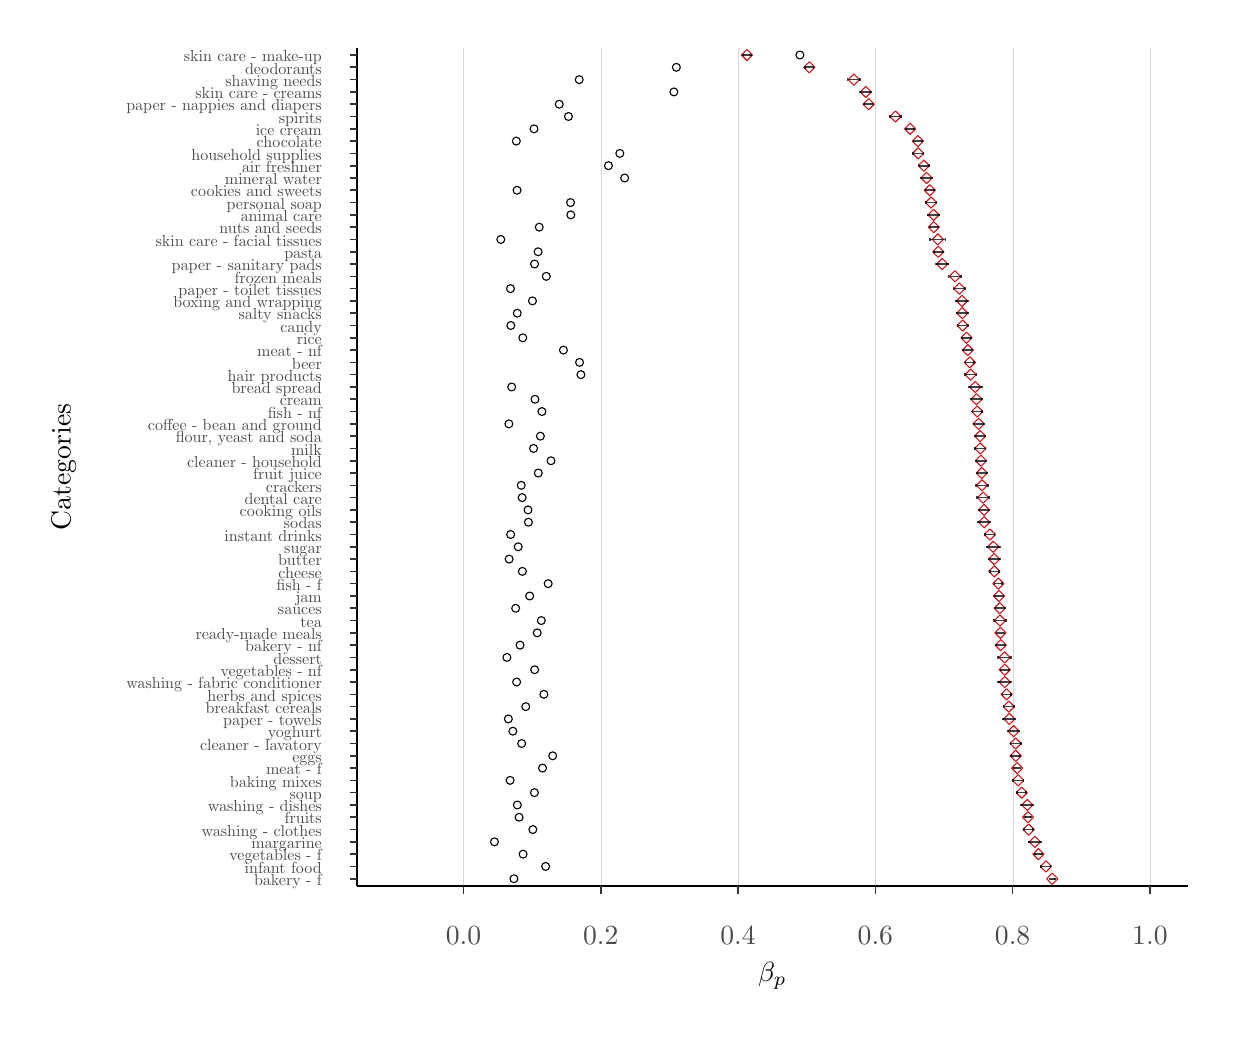
\begin{tikzpicture}[x=1pt,y=1pt]
\definecolor{fillColor}{RGB}{255,255,255}
\path[use as bounding box,fill=fillColor,fill opacity=0.00] (0,0) rectangle (433.62,361.35);
\begin{scope}
\path[clip] (  0.00,  0.00) rectangle (433.62,361.35);
\definecolor{drawColor}{RGB}{255,255,255}
\definecolor{fillColor}{RGB}{255,255,255}

\path[draw=drawColor,line width= 0.6pt,line join=round,line cap=round,fill=fillColor] (  0.00,  0.00) rectangle (433.62,361.35);
\end{scope}
\begin{scope}
\path[clip] (119.04, 51.15) rectangle (419.17,354.12);
\definecolor{drawColor}{RGB}{255,255,255}

\path[draw=drawColor,line width= 0.3pt,line join=round] (132.68, 51.15) --
	(132.68,354.12);

\path[draw=drawColor,line width= 0.3pt,line join=round] (182.29, 51.15) --
	(182.29,354.12);

\path[draw=drawColor,line width= 0.3pt,line join=round] (231.90, 51.15) --
	(231.90,354.12);

\path[draw=drawColor,line width= 0.3pt,line join=round] (281.51, 51.15) --
	(281.51,354.12);

\path[draw=drawColor,line width= 0.3pt,line join=round] (331.11, 51.15) --
	(331.11,354.12);

\path[draw=drawColor,line width= 0.3pt,line join=round] (380.72, 51.15) --
	(380.72,354.12);
\definecolor{drawColor}{gray}{0.85}

\path[draw=drawColor,line width= 0.1pt,line join=round] (157.49, 51.15) --
	(157.49,354.12);

\path[draw=drawColor,line width= 0.1pt,line join=round] (207.09, 51.15) --
	(207.09,354.12);

\path[draw=drawColor,line width= 0.1pt,line join=round] (256.70, 51.15) --
	(256.70,354.12);

\path[draw=drawColor,line width= 0.1pt,line join=round] (306.31, 51.15) --
	(306.31,354.12);

\path[draw=drawColor,line width= 0.1pt,line join=round] (355.92, 51.15) --
	(355.92,354.12);

\path[draw=drawColor,line width= 0.1pt,line join=round] (405.52, 51.15) --
	(405.52,354.12);
\definecolor{drawColor}{RGB}{0,0,0}

\path[draw=drawColor,line width= 0.4pt,line join=round,line cap=round] (209.86,311.48) circle (  1.43);

\path[draw=drawColor,line width= 0.4pt,line join=round,line cap=round] (196.26,293.71) circle (  1.43);

\path[draw=drawColor,line width= 0.4pt,line join=round,line cap=round] (175.71, 53.82) circle (  1.43);

\path[draw=drawColor,line width= 0.4pt,line join=round,line cap=round] (177.92,138.22) circle (  1.43);

\path[draw=drawColor,line width= 0.4pt,line join=round,line cap=round] (174.31, 89.36) circle (  1.43);

\path[draw=drawColor,line width= 0.4pt,line join=round,line cap=round] (199.42,240.40) circle (  1.43);

\path[draw=drawColor,line width= 0.4pt,line join=round,line cap=round] (182.40,262.61) circle (  1.43);

\path[draw=drawColor,line width= 0.4pt,line join=round,line cap=round] (174.89,231.51) circle (  1.43);

\path[draw=drawColor,line width= 0.4pt,line join=round,line cap=round] (179.98,116.01) circle (  1.43);

\path[draw=drawColor,line width= 0.4pt,line join=round,line cap=round] (173.98,169.32) circle (  1.43);

\path[draw=drawColor,line width= 0.4pt,line join=round,line cap=round] (174.58,253.73) circle (  1.43);

\path[draw=drawColor,line width= 0.4pt,line join=round,line cap=round] (178.76,164.88) circle (  1.43);

\path[draw=drawColor,line width= 0.4pt,line join=round,line cap=round] (176.57,320.36) circle (  1.43);

\path[draw=drawColor,line width= 0.4pt,line join=round,line cap=round] (189.10,204.86) circle (  1.43);

\path[draw=drawColor,line width= 0.4pt,line join=round,line cap=round] (178.50,102.69) circle (  1.43);

\path[draw=drawColor,line width= 0.4pt,line join=round,line cap=round] (173.89,218.19) circle (  1.43);

\path[draw=drawColor,line width= 0.4pt,line join=round,line cap=round] (176.84,302.59) circle (  1.43);

\path[draw=drawColor,line width= 0.4pt,line join=round,line cap=round] (180.79,187.09) circle (  1.43);

\path[draw=drawColor,line width= 0.4pt,line join=round,line cap=round] (178.36,195.97) circle (  1.43);

\path[draw=drawColor,line width= 0.4pt,line join=round,line cap=round] (183.31,227.07) circle (  1.43);

\path[draw=drawColor,line width= 0.4pt,line join=round,line cap=round] (178.67,191.53) circle (  1.43);

\path[draw=drawColor,line width= 0.4pt,line join=round,line cap=round] (234.40,347.02) circle (  1.43);

\path[draw=drawColor,line width= 0.4pt,line join=round,line cap=round] (173.16,133.78) circle (  1.43);

\path[draw=drawColor,line width= 0.4pt,line join=round,line cap=round] (189.72, 98.24) circle (  1.43);

\path[draw=drawColor,line width= 0.4pt,line join=round,line cap=round] (188.09,160.44) circle (  1.43);

\path[draw=drawColor,line width= 0.4pt,line join=round,line cap=round] (185.83,222.63) circle (  1.43);

\path[draw=drawColor,line width= 0.4pt,line join=round,line cap=round] (185.26,213.74) circle (  1.43);

\path[draw=drawColor,line width= 0.4pt,line join=round,line cap=round] (187.40,271.49) circle (  1.43);

\path[draw=drawColor,line width= 0.4pt,line join=round,line cap=round] (184.51,200.42) circle (  1.43);

\path[draw=drawColor,line width= 0.4pt,line join=round,line cap=round] (177.56, 76.03) circle (  1.43);

\path[draw=drawColor,line width= 0.4pt,line join=round,line cap=round] (199.91,235.96) circle (  1.43);

\path[draw=drawColor,line width= 0.4pt,line join=round,line cap=round] (186.53,120.45) circle (  1.43);

\path[draw=drawColor,line width= 0.4pt,line join=round,line cap=round] (213.97,315.92) circle (  1.43);

\path[draw=drawColor,line width= 0.4pt,line join=round,line cap=round] (182.96,324.80) circle (  1.43);

\path[draw=drawColor,line width= 0.4pt,line join=round,line cap=round] (187.16, 58.26) circle (  1.43);

\path[draw=drawColor,line width= 0.4pt,line join=round,line cap=round] (174.52,178.21) circle (  1.43);

\path[draw=drawColor,line width= 0.4pt,line join=round,line cap=round] (181.40,155.99) circle (  1.43);

\path[draw=drawColor,line width= 0.4pt,line join=round,line cap=round] (168.67, 67.15) circle (  1.43);

\path[draw=drawColor,line width= 0.4pt,line join=round,line cap=round] (186.04, 93.80) circle (  1.43);

\path[draw=drawColor,line width= 0.4pt,line join=round,line cap=round] (193.59,244.84) circle (  1.43);

\path[draw=drawColor,line width= 0.4pt,line join=round,line cap=round] (182.79,209.30) circle (  1.43);

\path[draw=drawColor,line width= 0.4pt,line join=round,line cap=round] (215.72,307.03) circle (  1.43);

\path[draw=drawColor,line width= 0.4pt,line join=round,line cap=round] (184.86,289.26) circle (  1.43);

\path[draw=drawColor,line width= 0.4pt,line join=round,line cap=round] (192.08,333.69) circle (  1.43);

\path[draw=drawColor,line width= 0.4pt,line join=round,line cap=round] (183.16,275.94) circle (  1.43);

\path[draw=drawColor,line width= 0.4pt,line join=round,line cap=round] (174.46,267.05) circle (  1.43);

\path[draw=drawColor,line width= 0.4pt,line join=round,line cap=round] (173.69,111.57) circle (  1.43);

\path[draw=drawColor,line width= 0.4pt,line join=round,line cap=round] (184.44,280.38) circle (  1.43);

\path[draw=drawColor,line width= 0.4pt,line join=round,line cap=round] (196.16,298.15) circle (  1.43);

\path[draw=drawColor,line width= 0.4pt,line join=round,line cap=round] (184.12,142.67) circle (  1.43);

\path[draw=drawColor,line width= 0.4pt,line join=round,line cap=round] (178.91,249.28) circle (  1.43);

\path[draw=drawColor,line width= 0.4pt,line join=round,line cap=round] (176.91,258.17) circle (  1.43);

\path[draw=drawColor,line width= 0.4pt,line join=round,line cap=round] (176.34,151.55) circle (  1.43);

\path[draw=drawColor,line width= 0.4pt,line join=round,line cap=round] (199.29,342.57) circle (  1.43);

\path[draw=drawColor,line width= 0.4pt,line join=round,line cap=round] (233.51,338.13) circle (  1.43);

\path[draw=drawColor,line width= 0.4pt,line join=round,line cap=round] (170.96,284.82) circle (  1.43);

\path[draw=drawColor,line width= 0.4pt,line join=round,line cap=round] (279.04,351.46) circle (  1.43);

\path[draw=drawColor,line width= 0.4pt,line join=round,line cap=round] (180.94,182.65) circle (  1.43);

\path[draw=drawColor,line width= 0.4pt,line join=round,line cap=round] (183.12, 84.92) circle (  1.43);

\path[draw=drawColor,line width= 0.4pt,line join=round,line cap=round] (195.42,329.25) circle (  1.43);

\path[draw=drawColor,line width= 0.4pt,line join=round,line cap=round] (177.24,173.76) circle (  1.43);

\path[draw=drawColor,line width= 0.4pt,line join=round,line cap=round] (185.59,147.11) circle (  1.43);

\path[draw=drawColor,line width= 0.4pt,line join=round,line cap=round] (179.01, 62.70) circle (  1.43);

\path[draw=drawColor,line width= 0.4pt,line join=round,line cap=round] (183.20,129.34) circle (  1.43);

\path[draw=drawColor,line width= 0.4pt,line join=round,line cap=round] (182.54, 71.59) circle (  1.43);

\path[draw=drawColor,line width= 0.4pt,line join=round,line cap=round] (176.94, 80.47) circle (  1.43);

\path[draw=drawColor,line width= 0.4pt,line join=round,line cap=round] (176.68,124.90) circle (  1.43);

\path[draw=drawColor,line width= 0.4pt,line join=round,line cap=round] (175.32,107.13) circle (  1.43);
\definecolor{drawColor}{RGB}{203,24,29}

\path[draw=drawColor,line width= 0.4pt,line join=round,line cap=round] (321.80,311.48) --
	(323.82,313.49) --
	(325.84,311.48) --
	(323.82,309.46) --
	cycle;

\path[draw=drawColor,line width= 0.4pt,line join=round,line cap=round] (325.32,293.71) --
	(327.33,295.72) --
	(329.35,293.71) --
	(327.33,291.69) --
	cycle;

\path[draw=drawColor,line width= 0.4pt,line join=round,line cap=round] (368.21, 53.82) --
	(370.23, 55.84) --
	(372.25, 53.82) --
	(370.23, 51.80) --
	cycle;

\path[draw=drawColor,line width= 0.4pt,line join=round,line cap=round] (349.60,138.22) --
	(351.61,140.24) --
	(353.63,138.22) --
	(351.61,136.21) --
	cycle;

\path[draw=drawColor,line width= 0.4pt,line join=round,line cap=round] (355.88, 89.36) --
	(357.90, 91.38) --
	(359.91, 89.36) --
	(357.90, 87.34) --
	cycle;

\path[draw=drawColor,line width= 0.4pt,line join=round,line cap=round] (338.41,240.40) --
	(340.43,242.42) --
	(342.45,240.40) --
	(340.43,238.38) --
	cycle;

\path[draw=drawColor,line width= 0.4pt,line join=round,line cap=round] (335.59,262.61) --
	(337.60,264.63) --
	(339.62,262.61) --
	(337.60,260.59) --
	cycle;

\path[draw=drawColor,line width= 0.4pt,line join=round,line cap=round] (340.39,231.51) --
	(342.41,233.53) --
	(344.43,231.51) --
	(342.41,229.50) --
	cycle;

\path[draw=drawColor,line width= 0.4pt,line join=round,line cap=round] (352.49,116.01) --
	(354.51,118.03) --
	(356.53,116.01) --
	(354.51,113.99) --
	cycle;

\path[draw=drawColor,line width= 0.4pt,line join=round,line cap=round] (347.23,169.32) --
	(349.25,171.34) --
	(351.27,169.32) --
	(349.25,167.30) --
	cycle;

\path[draw=drawColor,line width= 0.4pt,line join=round,line cap=round] (335.83,253.73) --
	(337.85,255.74) --
	(339.87,253.73) --
	(337.85,251.71) --
	cycle;

\path[draw=drawColor,line width= 0.4pt,line join=round,line cap=round] (347.27,164.88) --
	(349.29,166.90) --
	(351.31,164.88) --
	(349.29,162.86) --
	cycle;

\path[draw=drawColor,line width= 0.4pt,line join=round,line cap=round] (319.65,320.36) --
	(321.67,322.38) --
	(323.68,320.36) --
	(321.67,318.34) --
	cycle;

\path[draw=drawColor,line width= 0.4pt,line join=round,line cap=round] (342.48,204.86) --
	(344.50,206.88) --
	(346.51,204.86) --
	(344.50,202.84) --
	cycle;

\path[draw=drawColor,line width= 0.4pt,line join=round,line cap=round] (355.00,102.69) --
	(357.01,104.70) --
	(359.03,102.69) --
	(357.01,100.67) --
	cycle;

\path[draw=drawColor,line width= 0.4pt,line join=round,line cap=round] (341.61,218.19) --
	(343.63,220.20) --
	(345.65,218.19) --
	(343.63,216.17) --
	cycle;

\path[draw=drawColor,line width= 0.4pt,line join=round,line cap=round] (323.97,302.59) --
	(325.99,304.61) --
	(328.01,302.59) --
	(325.99,300.57) --
	cycle;

\path[draw=drawColor,line width= 0.4pt,line join=round,line cap=round] (343.59,187.09) --
	(345.60,189.11) --
	(347.62,187.09) --
	(345.60,185.07) --
	cycle;

\path[draw=drawColor,line width= 0.4pt,line join=round,line cap=round] (342.82,195.97) --
	(344.83,197.99) --
	(346.85,195.97) --
	(344.83,193.96) --
	cycle;

\path[draw=drawColor,line width= 0.4pt,line join=round,line cap=round] (340.84,227.07) --
	(342.86,229.09) --
	(344.87,227.07) --
	(342.86,225.05) --
	cycle;

\path[draw=drawColor,line width= 0.4pt,line join=round,line cap=round] (343.21,191.53) --
	(345.23,193.55) --
	(347.25,191.53) --
	(345.23,189.51) --
	cycle;

\path[draw=drawColor,line width= 0.4pt,line join=round,line cap=round] (280.42,347.02) --
	(282.44,349.03) --
	(284.45,347.02) --
	(282.44,345.00) --
	cycle;

\path[draw=drawColor,line width= 0.4pt,line join=round,line cap=round] (350.98,133.78) --
	(353.00,135.80) --
	(355.01,133.78) --
	(353.00,131.76) --
	cycle;

\path[draw=drawColor,line width= 0.4pt,line join=round,line cap=round] (355.00, 98.24) --
	(357.02,100.26) --
	(359.03, 98.24) --
	(357.02, 96.23) --
	cycle;

\path[draw=drawColor,line width= 0.4pt,line join=round,line cap=round] (348.73,160.44) --
	(350.75,162.45) --
	(352.77,160.44) --
	(350.75,158.42) --
	cycle;

\path[draw=drawColor,line width= 0.4pt,line join=round,line cap=round] (341.09,222.63) --
	(343.11,224.65) --
	(345.12,222.63) --
	(343.11,220.61) --
	cycle;

\path[draw=drawColor,line width= 0.4pt,line join=round,line cap=round] (342.16,213.74) --
	(344.18,215.76) --
	(346.19,213.74) --
	(344.18,211.73) --
	cycle;

\path[draw=drawColor,line width= 0.4pt,line join=round,line cap=round] (333.05,271.49) --
	(335.07,273.51) --
	(337.09,271.49) --
	(335.07,269.48) --
	cycle;

\path[draw=drawColor,line width= 0.4pt,line join=round,line cap=round] (342.75,200.42) --
	(344.77,202.43) --
	(346.78,200.42) --
	(344.77,198.40) --
	cycle;

\path[draw=drawColor,line width= 0.4pt,line join=round,line cap=round] (359.46, 76.03) --
	(361.48, 78.05) --
	(363.50, 76.03) --
	(361.48, 74.01) --
	cycle;

\path[draw=drawColor,line width= 0.4pt,line join=round,line cap=round] (338.73,235.96) --
	(340.75,237.97) --
	(342.76,235.96) --
	(340.75,233.94) --
	cycle;

\path[draw=drawColor,line width= 0.4pt,line join=round,line cap=round] (351.74,120.45) --
	(353.76,122.47) --
	(355.78,120.45) --
	(353.76,118.44) --
	cycle;

\path[draw=drawColor,line width= 0.4pt,line join=round,line cap=round] (319.78,315.92) --
	(321.80,317.94) --
	(323.82,315.92) --
	(321.80,313.90) --
	cycle;

\path[draw=drawColor,line width= 0.4pt,line join=round,line cap=round] (316.85,324.80) --
	(318.86,326.82) --
	(320.88,324.80) --
	(318.86,322.79) --
	cycle;

\path[draw=drawColor,line width= 0.4pt,line join=round,line cap=round] (365.93, 58.26) --
	(367.95, 60.28) --
	(369.96, 58.26) --
	(367.95, 56.24) --
	cycle;

\path[draw=drawColor,line width= 0.4pt,line join=round,line cap=round] (345.69,178.21) --
	(347.71,180.22) --
	(349.73,178.21) --
	(347.71,176.19) --
	cycle;

\path[draw=drawColor,line width= 0.4pt,line join=round,line cap=round] (348.98,155.99) --
	(351.00,158.01) --
	(353.02,155.99) --
	(351.00,153.98) --
	cycle;

\path[draw=drawColor,line width= 0.4pt,line join=round,line cap=round] (361.93, 67.15) --
	(363.94, 69.16) --
	(365.96, 67.15) --
	(363.94, 65.13) --
	cycle;

\path[draw=drawColor,line width= 0.4pt,line join=round,line cap=round] (355.54, 93.80) --
	(357.55, 95.82) --
	(359.57, 93.80) --
	(357.55, 91.78) --
	cycle;

\path[draw=drawColor,line width= 0.4pt,line join=round,line cap=round] (337.69,244.84) --
	(339.70,246.86) --
	(341.72,244.84) --
	(339.70,242.82) --
	cycle;

\path[draw=drawColor,line width= 0.4pt,line join=round,line cap=round] (342.22,209.30) --
	(344.24,211.32) --
	(346.25,209.30) --
	(344.24,207.28) --
	cycle;

\path[draw=drawColor,line width= 0.4pt,line join=round,line cap=round] (322.78,307.03) --
	(324.80,309.05) --
	(326.82,307.03) --
	(324.80,305.02) --
	cycle;

\path[draw=drawColor,line width= 0.4pt,line join=round,line cap=round] (325.40,289.26) --
	(327.42,291.28) --
	(329.44,289.26) --
	(327.42,287.25) --
	cycle;

\path[draw=drawColor,line width= 0.4pt,line join=round,line cap=round] (301.89,333.69) --
	(303.91,335.71) --
	(305.93,333.69) --
	(303.91,331.67) --
	cycle;

\path[draw=drawColor,line width= 0.4pt,line join=round,line cap=round] (328.47,275.94) --
	(330.49,277.95) --
	(332.50,275.94) --
	(330.49,273.92) --
	cycle;

\path[draw=drawColor,line width= 0.4pt,line join=round,line cap=round] (334.65,267.05) --
	(336.67,269.07) --
	(338.69,267.05) --
	(336.67,265.04) --
	cycle;

\path[draw=drawColor,line width= 0.4pt,line join=round,line cap=round] (352.69,111.57) --
	(354.71,113.59) --
	(356.73,111.57) --
	(354.71,109.55) --
	cycle;

\path[draw=drawColor,line width= 0.4pt,line join=round,line cap=round] (327.02,280.38) --
	(329.04,282.40) --
	(331.06,280.38) --
	(329.04,278.36) --
	cycle;

\path[draw=drawColor,line width= 0.4pt,line join=round,line cap=round] (324.40,298.15) --
	(326.42,300.17) --
	(328.44,298.15) --
	(326.42,296.13) --
	cycle;

\path[draw=drawColor,line width= 0.4pt,line join=round,line cap=round] (349.48,142.67) --
	(351.50,144.68) --
	(353.52,142.67) --
	(351.50,140.65) --
	cycle;

\path[draw=drawColor,line width= 0.4pt,line join=round,line cap=round] (337.22,249.28) --
	(339.24,251.30) --
	(341.26,249.28) --
	(339.24,247.27) --
	cycle;

\path[draw=drawColor,line width= 0.4pt,line join=round,line cap=round] (335.72,258.17) --
	(337.74,260.19) --
	(339.76,258.17) --
	(337.74,256.15) --
	cycle;

\path[draw=drawColor,line width= 0.4pt,line join=round,line cap=round] (349.27,151.55) --
	(351.29,153.57) --
	(353.30,151.55) --
	(351.29,149.53) --
	cycle;

\path[draw=drawColor,line width= 0.4pt,line join=round,line cap=round] (296.53,342.57) --
	(298.55,344.59) --
	(300.57,342.57) --
	(298.55,340.56) --
	cycle;

\path[draw=drawColor,line width= 0.4pt,line join=round,line cap=round] (300.82,338.13) --
	(302.84,340.15) --
	(304.85,338.13) --
	(302.84,336.11) --
	cycle;

\path[draw=drawColor,line width= 0.4pt,line join=round,line cap=round] (326.89,284.82) --
	(328.90,286.84) --
	(330.92,284.82) --
	(328.90,282.80) --
	cycle;

\path[draw=drawColor,line width= 0.4pt,line join=round,line cap=round] (257.85,351.46) --
	(259.87,353.48) --
	(261.89,351.46) --
	(259.87,349.44) --
	cycle;

\path[draw=drawColor,line width= 0.4pt,line join=round,line cap=round] (343.61,182.65) --
	(345.63,184.67) --
	(347.65,182.65) --
	(345.63,180.63) --
	cycle;

\path[draw=drawColor,line width= 0.4pt,line join=round,line cap=round] (357.18, 84.92) --
	(359.20, 86.93) --
	(361.22, 84.92) --
	(359.20, 82.90) --
	cycle;

\path[draw=drawColor,line width= 0.4pt,line join=round,line cap=round] (311.54,329.25) --
	(313.55,331.26) --
	(315.57,329.25) --
	(313.55,327.23) --
	cycle;

\path[draw=drawColor,line width= 0.4pt,line join=round,line cap=round] (346.90,173.76) --
	(348.92,175.78) --
	(350.93,173.76) --
	(348.92,171.75) --
	cycle;

\path[draw=drawColor,line width= 0.4pt,line join=round,line cap=round] (349.32,147.11) --
	(351.33,149.13) --
	(353.35,147.11) --
	(351.33,145.09) --
	cycle;

\path[draw=drawColor,line width= 0.4pt,line join=round,line cap=round] (363.23, 62.70) --
	(365.24, 64.72) --
	(367.26, 62.70) --
	(365.24, 60.69) --
	cycle;

\path[draw=drawColor,line width= 0.4pt,line join=round,line cap=round] (351.03,129.34) --
	(353.04,131.36) --
	(355.06,129.34) --
	(353.04,127.32) --
	cycle;

\path[draw=drawColor,line width= 0.4pt,line join=round,line cap=round] (359.70, 71.59) --
	(361.71, 73.61) --
	(363.73, 71.59) --
	(361.71, 69.57) --
	cycle;

\path[draw=drawColor,line width= 0.4pt,line join=round,line cap=round] (359.21, 80.47) --
	(361.23, 82.49) --
	(363.24, 80.47) --
	(361.23, 78.46) --
	cycle;

\path[draw=drawColor,line width= 0.4pt,line join=round,line cap=round] (351.04,124.90) --
	(353.06,126.91) --
	(355.08,124.90) --
	(353.06,122.88) --
	cycle;

\path[draw=drawColor,line width= 0.4pt,line join=round,line cap=round] (354.25,107.13) --
	(356.27,109.14) --
	(358.29,107.13) --
	(356.27,105.11) --
	cycle;
\definecolor{drawColor}{RGB}{0,0,0}

\path[draw=drawColor,draw opacity=0.75,line width= 0.6pt,line join=round] (325.70,311.03) --
	(325.70,311.92);

\path[draw=drawColor,draw opacity=0.75,line width= 0.6pt,line join=round] (325.70,311.48) --
	(321.94,311.48);

\path[draw=drawColor,draw opacity=0.75,line width= 0.6pt,line join=round] (321.94,311.03) --
	(321.94,311.92);

\path[draw=drawColor,draw opacity=0.75,line width= 0.6pt,line join=round] (329.53,293.26) --
	(329.53,294.15);

\path[draw=drawColor,draw opacity=0.75,line width= 0.6pt,line join=round] (329.53,293.71) --
	(325.14,293.71);

\path[draw=drawColor,draw opacity=0.75,line width= 0.6pt,line join=round] (325.14,293.26) --
	(325.14,294.15);

\path[draw=drawColor,draw opacity=0.75,line width= 0.6pt,line join=round] (371.21, 53.37) --
	(371.21, 54.26);

\path[draw=drawColor,draw opacity=0.75,line width= 0.6pt,line join=round] (371.21, 53.82) --
	(369.24, 53.82);

\path[draw=drawColor,draw opacity=0.75,line width= 0.6pt,line join=round] (369.24, 53.37) --
	(369.24, 54.26);

\path[draw=drawColor,draw opacity=0.75,line width= 0.6pt,line join=round] (353.38,137.78) --
	(353.38,138.67);

\path[draw=drawColor,draw opacity=0.75,line width= 0.6pt,line join=round] (353.38,138.22) --
	(349.84,138.22);

\path[draw=drawColor,draw opacity=0.75,line width= 0.6pt,line join=round] (349.84,137.78) --
	(349.84,138.67);

\path[draw=drawColor,draw opacity=0.75,line width= 0.6pt,line join=round] (359.82, 88.91) --
	(359.82, 89.80);

\path[draw=drawColor,draw opacity=0.75,line width= 0.6pt,line join=round] (359.82, 89.36) --
	(355.97, 89.36);

\path[draw=drawColor,draw opacity=0.75,line width= 0.6pt,line join=round] (355.97, 88.91) --
	(355.97, 89.80);

\path[draw=drawColor,draw opacity=0.75,line width= 0.6pt,line join=round] (342.00,239.95) --
	(342.00,240.84);

\path[draw=drawColor,draw opacity=0.75,line width= 0.6pt,line join=round] (342.00,240.40) --
	(338.85,240.40);

\path[draw=drawColor,draw opacity=0.75,line width= 0.6pt,line join=round] (338.85,239.95) --
	(338.85,240.84);

\path[draw=drawColor,draw opacity=0.75,line width= 0.6pt,line join=round] (339.73,262.17) --
	(339.73,263.05);

\path[draw=drawColor,draw opacity=0.75,line width= 0.6pt,line join=round] (339.73,262.61) --
	(335.48,262.61);

\path[draw=drawColor,draw opacity=0.75,line width= 0.6pt,line join=round] (335.48,262.17) --
	(335.48,263.05);

\path[draw=drawColor,draw opacity=0.75,line width= 0.6pt,line join=round] (344.75,231.07) --
	(344.75,231.96);

\path[draw=drawColor,draw opacity=0.75,line width= 0.6pt,line join=round] (344.75,231.51) --
	(340.07,231.51);

\path[draw=drawColor,draw opacity=0.75,line width= 0.6pt,line join=round] (340.07,231.07) --
	(340.07,231.96);

\path[draw=drawColor,draw opacity=0.75,line width= 0.6pt,line join=round] (356.46,115.57) --
	(356.46,116.46);

\path[draw=drawColor,draw opacity=0.75,line width= 0.6pt,line join=round] (356.46,116.01) --
	(352.56,116.01);

\path[draw=drawColor,draw opacity=0.75,line width= 0.6pt,line join=round] (352.56,115.57) --
	(352.56,116.46);

\path[draw=drawColor,draw opacity=0.75,line width= 0.6pt,line join=round] (351.28,168.88) --
	(351.28,169.76);

\path[draw=drawColor,draw opacity=0.75,line width= 0.6pt,line join=round] (351.28,169.32) --
	(347.22,169.32);

\path[draw=drawColor,draw opacity=0.75,line width= 0.6pt,line join=round] (347.22,168.88) --
	(347.22,169.76);

\path[draw=drawColor,draw opacity=0.75,line width= 0.6pt,line join=round] (339.69,253.28) --
	(339.69,254.17);

\path[draw=drawColor,draw opacity=0.75,line width= 0.6pt,line join=round] (339.69,253.73) --
	(336.01,253.73);

\path[draw=drawColor,draw opacity=0.75,line width= 0.6pt,line join=round] (336.01,253.28) --
	(336.01,254.17);

\path[draw=drawColor,draw opacity=0.75,line width= 0.6pt,line join=round] (350.88,164.43) --
	(350.88,165.32);

\path[draw=drawColor,draw opacity=0.75,line width= 0.6pt,line join=round] (350.88,164.88) --
	(347.70,164.88);

\path[draw=drawColor,draw opacity=0.75,line width= 0.6pt,line join=round] (347.70,164.43) --
	(347.70,165.32);

\path[draw=drawColor,draw opacity=0.75,line width= 0.6pt,line join=round] (323.27,319.92) --
	(323.27,320.81);

\path[draw=drawColor,draw opacity=0.75,line width= 0.6pt,line join=round] (323.27,320.36) --
	(320.07,320.36);

\path[draw=drawColor,draw opacity=0.75,line width= 0.6pt,line join=round] (320.07,319.92) --
	(320.07,320.81);

\path[draw=drawColor,draw opacity=0.75,line width= 0.6pt,line join=round] (346.21,204.42) --
	(346.21,205.30);

\path[draw=drawColor,draw opacity=0.75,line width= 0.6pt,line join=round] (346.21,204.86) --
	(342.78,204.86);

\path[draw=drawColor,draw opacity=0.75,line width= 0.6pt,line join=round] (342.78,204.42) --
	(342.78,205.30);

\path[draw=drawColor,draw opacity=0.75,line width= 0.6pt,line join=round] (358.93,102.24) --
	(358.93,103.13);

\path[draw=drawColor,draw opacity=0.75,line width= 0.6pt,line join=round] (358.93,102.69) --
	(355.10,102.69);

\path[draw=drawColor,draw opacity=0.75,line width= 0.6pt,line join=round] (355.10,102.24) --
	(355.10,103.13);

\path[draw=drawColor,draw opacity=0.75,line width= 0.6pt,line join=round] (345.51,217.74) --
	(345.51,218.63);

\path[draw=drawColor,draw opacity=0.75,line width= 0.6pt,line join=round] (345.51,218.19) --
	(341.75,218.19);

\path[draw=drawColor,draw opacity=0.75,line width= 0.6pt,line join=round] (341.75,217.74) --
	(341.75,218.63);

\path[draw=drawColor,draw opacity=0.75,line width= 0.6pt,line join=round] (327.58,302.15) --
	(327.58,303.04);

\path[draw=drawColor,draw opacity=0.75,line width= 0.6pt,line join=round] (327.58,302.59) --
	(324.39,302.59);

\path[draw=drawColor,draw opacity=0.75,line width= 0.6pt,line join=round] (324.39,302.15) --
	(324.39,303.04);

\path[draw=drawColor,draw opacity=0.75,line width= 0.6pt,line join=round] (347.39,186.65) --
	(347.39,187.53);

\path[draw=drawColor,draw opacity=0.75,line width= 0.6pt,line join=round] (347.39,187.09) --
	(343.81,187.09);

\path[draw=drawColor,draw opacity=0.75,line width= 0.6pt,line join=round] (343.81,186.65) --
	(343.81,187.53);

\path[draw=drawColor,draw opacity=0.75,line width= 0.6pt,line join=round] (346.93,195.53) --
	(346.93,196.42);

\path[draw=drawColor,draw opacity=0.75,line width= 0.6pt,line join=round] (346.93,195.97) --
	(342.74,195.97);

\path[draw=drawColor,draw opacity=0.75,line width= 0.6pt,line join=round] (342.74,195.53) --
	(342.74,196.42);

\path[draw=drawColor,draw opacity=0.75,line width= 0.6pt,line join=round] (344.95,226.63) --
	(344.95,227.52);

\path[draw=drawColor,draw opacity=0.75,line width= 0.6pt,line join=round] (344.95,227.07) --
	(340.76,227.07);

\path[draw=drawColor,draw opacity=0.75,line width= 0.6pt,line join=round] (340.76,226.63) --
	(340.76,227.52);

\path[draw=drawColor,draw opacity=0.75,line width= 0.6pt,line join=round] (347.34,191.09) --
	(347.34,191.98);

\path[draw=drawColor,draw opacity=0.75,line width= 0.6pt,line join=round] (347.34,191.53) --
	(343.12,191.53);

\path[draw=drawColor,draw opacity=0.75,line width= 0.6pt,line join=round] (343.12,191.09) --
	(343.12,191.98);

\path[draw=drawColor,draw opacity=0.75,line width= 0.6pt,line join=round] (284.01,346.57) --
	(284.01,347.46);

\path[draw=drawColor,draw opacity=0.75,line width= 0.6pt,line join=round] (284.01,347.02) --
	(280.86,347.02);

\path[draw=drawColor,draw opacity=0.75,line width= 0.6pt,line join=round] (280.86,346.57) --
	(280.86,347.46);

\path[draw=drawColor,draw opacity=0.75,line width= 0.6pt,line join=round] (355.30,133.34) --
	(355.30,134.23);

\path[draw=drawColor,draw opacity=0.75,line width= 0.6pt,line join=round] (355.30,133.78) --
	(350.69,133.78);

\path[draw=drawColor,draw opacity=0.75,line width= 0.6pt,line join=round] (350.69,133.34) --
	(350.69,134.23);

\path[draw=drawColor,draw opacity=0.75,line width= 0.6pt,line join=round] (358.68, 97.80) --
	(358.68, 98.69);

\path[draw=drawColor,draw opacity=0.75,line width= 0.6pt,line join=round] (358.68, 98.24) --
	(355.36, 98.24);

\path[draw=drawColor,draw opacity=0.75,line width= 0.6pt,line join=round] (355.36, 97.80) --
	(355.36, 98.69);

\path[draw=drawColor,draw opacity=0.75,line width= 0.6pt,line join=round] (352.14,159.99) --
	(352.14,160.88);

\path[draw=drawColor,draw opacity=0.75,line width= 0.6pt,line join=round] (352.14,160.44) --
	(349.36,160.44);

\path[draw=drawColor,draw opacity=0.75,line width= 0.6pt,line join=round] (349.36,159.99) --
	(349.36,160.88);

\path[draw=drawColor,draw opacity=0.75,line width= 0.6pt,line join=round] (344.77,222.18) --
	(344.77,223.07);

\path[draw=drawColor,draw opacity=0.75,line width= 0.6pt,line join=round] (344.77,222.63) --
	(341.44,222.63);

\path[draw=drawColor,draw opacity=0.75,line width= 0.6pt,line join=round] (341.44,222.18) --
	(341.44,223.07);

\path[draw=drawColor,draw opacity=0.75,line width= 0.6pt,line join=round] (346.04,213.30) --
	(346.04,214.19);

\path[draw=drawColor,draw opacity=0.75,line width= 0.6pt,line join=round] (346.04,213.74) --
	(342.31,213.74);

\path[draw=drawColor,draw opacity=0.75,line width= 0.6pt,line join=round] (342.31,213.30) --
	(342.31,214.19);

\path[draw=drawColor,draw opacity=0.75,line width= 0.6pt,line join=round] (337.36,271.05) --
	(337.36,271.94);

\path[draw=drawColor,draw opacity=0.75,line width= 0.6pt,line join=round] (337.36,271.49) --
	(332.78,271.49);

\path[draw=drawColor,draw opacity=0.75,line width= 0.6pt,line join=round] (332.78,271.05) --
	(332.78,271.94);

\path[draw=drawColor,draw opacity=0.75,line width= 0.6pt,line join=round] (346.64,199.97) --
	(346.64,200.86);

\path[draw=drawColor,draw opacity=0.75,line width= 0.6pt,line join=round] (346.64,200.42) --
	(342.89,200.42);

\path[draw=drawColor,draw opacity=0.75,line width= 0.6pt,line join=round] (342.89,199.97) --
	(342.89,200.86);

\path[draw=drawColor,draw opacity=0.75,line width= 0.6pt,line join=round] (362.53, 75.59) --
	(362.53, 76.48);

\path[draw=drawColor,draw opacity=0.75,line width= 0.6pt,line join=round] (362.53, 76.03) --
	(360.43, 76.03);

\path[draw=drawColor,draw opacity=0.75,line width= 0.6pt,line join=round] (360.43, 75.59) --
	(360.43, 76.48);

\path[draw=drawColor,draw opacity=0.75,line width= 0.6pt,line join=round] (342.82,235.51) --
	(342.82,236.40);

\path[draw=drawColor,draw opacity=0.75,line width= 0.6pt,line join=round] (342.82,235.96) --
	(338.67,235.96);

\path[draw=drawColor,draw opacity=0.75,line width= 0.6pt,line join=round] (338.67,235.51) --
	(338.67,236.40);

\path[draw=drawColor,draw opacity=0.75,line width= 0.6pt,line join=round] (355.27,120.01) --
	(355.27,120.90);

\path[draw=drawColor,draw opacity=0.75,line width= 0.6pt,line join=round] (355.27,120.45) --
	(352.25,120.45);

\path[draw=drawColor,draw opacity=0.75,line width= 0.6pt,line join=round] (352.25,120.01) --
	(352.25,120.90);

\path[draw=drawColor,draw opacity=0.75,line width= 0.6pt,line join=round] (323.71,315.47) --
	(323.71,316.36);

\path[draw=drawColor,draw opacity=0.75,line width= 0.6pt,line join=round] (323.71,315.92) --
	(319.89,315.92);

\path[draw=drawColor,draw opacity=0.75,line width= 0.6pt,line join=round] (319.89,315.47) --
	(319.89,316.36);

\path[draw=drawColor,draw opacity=0.75,line width= 0.6pt,line join=round] (320.35,324.36) --
	(320.35,325.25);

\path[draw=drawColor,draw opacity=0.75,line width= 0.6pt,line join=round] (320.35,324.80) --
	(317.38,324.80);

\path[draw=drawColor,draw opacity=0.75,line width= 0.6pt,line join=round] (317.38,324.36) --
	(317.38,325.25);

\path[draw=drawColor,draw opacity=0.75,line width= 0.6pt,line join=round] (369.65, 57.82) --
	(369.65, 58.71);

\path[draw=drawColor,draw opacity=0.75,line width= 0.6pt,line join=round] (369.65, 58.26) --
	(366.24, 58.26);

\path[draw=drawColor,draw opacity=0.75,line width= 0.6pt,line join=round] (366.24, 57.82) --
	(366.24, 58.71);

\path[draw=drawColor,draw opacity=0.75,line width= 0.6pt,line join=round] (349.39,177.76) --
	(349.39,178.65);

\path[draw=drawColor,draw opacity=0.75,line width= 0.6pt,line join=round] (349.39,178.21) --
	(346.03,178.21);

\path[draw=drawColor,draw opacity=0.75,line width= 0.6pt,line join=round] (346.03,177.76) --
	(346.03,178.65);

\path[draw=drawColor,draw opacity=0.75,line width= 0.6pt,line join=round] (352.66,155.55) --
	(352.66,156.44);

\path[draw=drawColor,draw opacity=0.75,line width= 0.6pt,line join=round] (352.66,155.99) --
	(349.34,155.99);

\path[draw=drawColor,draw opacity=0.75,line width= 0.6pt,line join=round] (349.34,155.55) --
	(349.34,156.44);

\path[draw=drawColor,draw opacity=0.75,line width= 0.6pt,line join=round] (366.29, 66.70) --
	(366.29, 67.59);

\path[draw=drawColor,draw opacity=0.75,line width= 0.6pt,line join=round] (366.29, 67.15) --
	(361.60, 67.15);

\path[draw=drawColor,draw opacity=0.75,line width= 0.6pt,line join=round] (361.60, 66.70) --
	(361.60, 67.59);

\path[draw=drawColor,draw opacity=0.75,line width= 0.6pt,line join=round] (358.71, 93.36) --
	(358.71, 94.24);

\path[draw=drawColor,draw opacity=0.75,line width= 0.6pt,line join=round] (358.71, 93.80) --
	(356.40, 93.80);

\path[draw=drawColor,draw opacity=0.75,line width= 0.6pt,line join=round] (356.40, 93.36) --
	(356.40, 94.24);

\path[draw=drawColor,draw opacity=0.75,line width= 0.6pt,line join=round] (341.39,244.40) --
	(341.39,245.29);

\path[draw=drawColor,draw opacity=0.75,line width= 0.6pt,line join=round] (341.39,244.84) --
	(338.01,244.84);

\path[draw=drawColor,draw opacity=0.75,line width= 0.6pt,line join=round] (338.01,244.40) --
	(338.01,245.29);

\path[draw=drawColor,draw opacity=0.75,line width= 0.6pt,line join=round] (346.15,208.86) --
	(346.15,209.75);

\path[draw=drawColor,draw opacity=0.75,line width= 0.6pt,line join=round] (346.15,209.30) --
	(342.32,209.30);

\path[draw=drawColor,draw opacity=0.75,line width= 0.6pt,line join=round] (342.32,208.86) --
	(342.32,209.75);

\path[draw=drawColor,draw opacity=0.75,line width= 0.6pt,line join=round] (326.94,306.59) --
	(326.94,307.48);

\path[draw=drawColor,draw opacity=0.75,line width= 0.6pt,line join=round] (326.94,307.03) --
	(322.65,307.03);

\path[draw=drawColor,draw opacity=0.75,line width= 0.6pt,line join=round] (322.65,306.59) --
	(322.65,307.48);

\path[draw=drawColor,draw opacity=0.75,line width= 0.6pt,line join=round] (328.86,288.82) --
	(328.86,289.71);

\path[draw=drawColor,draw opacity=0.75,line width= 0.6pt,line join=round] (328.86,289.26) --
	(325.99,289.26);

\path[draw=drawColor,draw opacity=0.75,line width= 0.6pt,line join=round] (325.99,288.82) --
	(325.99,289.71);

\path[draw=drawColor,draw opacity=0.75,line width= 0.6pt,line join=round] (305.58,333.24) --
	(305.58,334.13);

\path[draw=drawColor,draw opacity=0.75,line width= 0.6pt,line join=round] (305.58,333.69) --
	(302.24,333.69);

\path[draw=drawColor,draw opacity=0.75,line width= 0.6pt,line join=round] (302.24,333.24) --
	(302.24,334.13);

\path[draw=drawColor,draw opacity=0.75,line width= 0.6pt,line join=round] (332.74,275.49) --
	(332.74,276.38);

\path[draw=drawColor,draw opacity=0.75,line width= 0.6pt,line join=round] (332.74,275.94) --
	(328.23,275.94);

\path[draw=drawColor,draw opacity=0.75,line width= 0.6pt,line join=round] (328.23,275.49) --
	(328.23,276.38);

\path[draw=drawColor,draw opacity=0.75,line width= 0.6pt,line join=round] (338.75,266.61) --
	(338.75,267.50);

\path[draw=drawColor,draw opacity=0.75,line width= 0.6pt,line join=round] (338.75,267.05) --
	(334.60,267.05);

\path[draw=drawColor,draw opacity=0.75,line width= 0.6pt,line join=round] (334.60,266.61) --
	(334.60,267.50);

\path[draw=drawColor,draw opacity=0.75,line width= 0.6pt,line join=round] (356.91,111.13) --
	(356.91,112.01);

\path[draw=drawColor,draw opacity=0.75,line width= 0.6pt,line join=round] (356.91,111.57) --
	(352.51,111.57);

\path[draw=drawColor,draw opacity=0.75,line width= 0.6pt,line join=round] (352.51,111.13) --
	(352.51,112.01);

\path[draw=drawColor,draw opacity=0.75,line width= 0.6pt,line join=round] (330.67,279.94) --
	(330.67,280.82);

\path[draw=drawColor,draw opacity=0.75,line width= 0.6pt,line join=round] (330.67,280.38) --
	(327.41,280.38);

\path[draw=drawColor,draw opacity=0.75,line width= 0.6pt,line join=round] (327.41,279.94) --
	(327.41,280.82);

\path[draw=drawColor,draw opacity=0.75,line width= 0.6pt,line join=round] (328.34,297.70) --
	(328.34,298.59);

\path[draw=drawColor,draw opacity=0.75,line width= 0.6pt,line join=round] (328.34,298.15) --
	(324.50,298.15);

\path[draw=drawColor,draw opacity=0.75,line width= 0.6pt,line join=round] (324.50,297.70) --
	(324.50,298.59);

\path[draw=drawColor,draw opacity=0.75,line width= 0.6pt,line join=round] (352.91,142.22) --
	(352.91,143.11);

\path[draw=drawColor,draw opacity=0.75,line width= 0.6pt,line join=round] (352.91,142.67) --
	(350.10,142.67);

\path[draw=drawColor,draw opacity=0.75,line width= 0.6pt,line join=round] (350.10,142.22) --
	(350.10,143.11);

\path[draw=drawColor,draw opacity=0.75,line width= 0.6pt,line join=round] (340.76,248.84) --
	(340.76,249.73);

\path[draw=drawColor,draw opacity=0.75,line width= 0.6pt,line join=round] (340.76,249.28) --
	(337.71,249.28);

\path[draw=drawColor,draw opacity=0.75,line width= 0.6pt,line join=round] (337.71,248.84) --
	(337.71,249.73);

\path[draw=drawColor,draw opacity=0.75,line width= 0.6pt,line join=round] (339.90,257.72) --
	(339.90,258.61);

\path[draw=drawColor,draw opacity=0.75,line width= 0.6pt,line join=round] (339.90,258.17) --
	(335.59,258.17);

\path[draw=drawColor,draw opacity=0.75,line width= 0.6pt,line join=round] (335.59,257.72) --
	(335.59,258.61);

\path[draw=drawColor,draw opacity=0.75,line width= 0.6pt,line join=round] (353.10,151.11) --
	(353.10,152.00);

\path[draw=drawColor,draw opacity=0.75,line width= 0.6pt,line join=round] (353.10,151.55) --
	(349.47,151.55);

\path[draw=drawColor,draw opacity=0.75,line width= 0.6pt,line join=round] (349.47,151.11) --
	(349.47,152.00);

\path[draw=drawColor,draw opacity=0.75,line width= 0.6pt,line join=round] (300.83,342.13) --
	(300.83,343.02);

\path[draw=drawColor,draw opacity=0.75,line width= 0.6pt,line join=round] (300.83,342.57) --
	(296.27,342.57);

\path[draw=drawColor,draw opacity=0.75,line width= 0.6pt,line join=round] (296.27,342.13) --
	(296.27,343.02);

\path[draw=drawColor,draw opacity=0.75,line width= 0.6pt,line join=round] (304.80,337.69) --
	(304.80,338.57);

\path[draw=drawColor,draw opacity=0.75,line width= 0.6pt,line join=round] (304.80,338.13) --
	(300.87,338.13);

\path[draw=drawColor,draw opacity=0.75,line width= 0.6pt,line join=round] (300.87,337.69) --
	(300.87,338.57);

\path[draw=drawColor,draw opacity=0.75,line width= 0.6pt,line join=round] (331.65,284.38) --
	(331.65,285.27);

\path[draw=drawColor,draw opacity=0.75,line width= 0.6pt,line join=round] (331.65,284.82) --
	(326.16,284.82);

\path[draw=drawColor,draw opacity=0.75,line width= 0.6pt,line join=round] (326.16,284.38) --
	(326.16,285.27);

\path[draw=drawColor,draw opacity=0.75,line width= 0.6pt,line join=round] (261.34,351.01) --
	(261.34,351.90);

\path[draw=drawColor,draw opacity=0.75,line width= 0.6pt,line join=round] (261.34,351.46) --
	(258.40,351.46);

\path[draw=drawColor,draw opacity=0.75,line width= 0.6pt,line join=round] (258.40,351.01) --
	(258.40,351.90);

\path[draw=drawColor,draw opacity=0.75,line width= 0.6pt,line join=round] (347.75,182.20) --
	(347.75,183.09);

\path[draw=drawColor,draw opacity=0.75,line width= 0.6pt,line join=round] (347.75,182.65) --
	(343.51,182.65);

\path[draw=drawColor,draw opacity=0.75,line width= 0.6pt,line join=round] (343.51,182.20) --
	(343.51,183.09);

\path[draw=drawColor,draw opacity=0.75,line width= 0.6pt,line join=round] (360.84, 84.47) --
	(360.84, 85.36);

\path[draw=drawColor,draw opacity=0.75,line width= 0.6pt,line join=round] (360.84, 84.92) --
	(357.56, 84.92);

\path[draw=drawColor,draw opacity=0.75,line width= 0.6pt,line join=round] (357.56, 84.47) --
	(357.56, 85.36);

\path[draw=drawColor,draw opacity=0.75,line width= 0.6pt,line join=round] (315.53,328.80) --
	(315.53,329.69);

\path[draw=drawColor,draw opacity=0.75,line width= 0.6pt,line join=round] (315.53,329.25) --
	(311.57,329.25);

\path[draw=drawColor,draw opacity=0.75,line width= 0.6pt,line join=round] (311.57,328.80) --
	(311.57,329.69);

\path[draw=drawColor,draw opacity=0.75,line width= 0.6pt,line join=round] (351.27,173.32) --
	(351.27,174.21);

\path[draw=drawColor,draw opacity=0.75,line width= 0.6pt,line join=round] (351.27,173.76) --
	(346.56,173.76);

\path[draw=drawColor,draw opacity=0.75,line width= 0.6pt,line join=round] (346.56,173.32) --
	(346.56,174.21);

\path[draw=drawColor,draw opacity=0.75,line width= 0.6pt,line join=round] (353.56,146.66) --
	(353.56,147.55);

\path[draw=drawColor,draw opacity=0.75,line width= 0.6pt,line join=round] (353.56,147.11) --
	(349.10,147.11);

\path[draw=drawColor,draw opacity=0.75,line width= 0.6pt,line join=round] (349.10,146.66) --
	(349.10,147.55);

\path[draw=drawColor,draw opacity=0.75,line width= 0.6pt,line join=round] (366.55, 62.26) --
	(366.55, 63.15);

\path[draw=drawColor,draw opacity=0.75,line width= 0.6pt,line join=round] (366.55, 62.70) --
	(363.94, 62.70);

\path[draw=drawColor,draw opacity=0.75,line width= 0.6pt,line join=round] (363.94, 62.26) --
	(363.94, 63.15);

\path[draw=drawColor,draw opacity=0.75,line width= 0.6pt,line join=round] (354.59,128.90) --
	(354.59,129.78);

\path[draw=drawColor,draw opacity=0.75,line width= 0.6pt,line join=round] (354.59,129.34) --
	(351.50,129.34);

\path[draw=drawColor,draw opacity=0.75,line width= 0.6pt,line join=round] (351.50,128.90) --
	(351.50,129.78);

\path[draw=drawColor,draw opacity=0.75,line width= 0.6pt,line join=round] (363.33, 71.14) --
	(363.33, 72.03);

\path[draw=drawColor,draw opacity=0.75,line width= 0.6pt,line join=round] (363.33, 71.59) --
	(360.10, 71.59);

\path[draw=drawColor,draw opacity=0.75,line width= 0.6pt,line join=round] (360.10, 71.14) --
	(360.10, 72.03);

\path[draw=drawColor,draw opacity=0.75,line width= 0.6pt,line join=round] (363.43, 80.03) --
	(363.43, 80.92);

\path[draw=drawColor,draw opacity=0.75,line width= 0.6pt,line join=round] (363.43, 80.47) --
	(359.02, 80.47);

\path[draw=drawColor,draw opacity=0.75,line width= 0.6pt,line join=round] (359.02, 80.03) --
	(359.02, 80.92);

\path[draw=drawColor,draw opacity=0.75,line width= 0.6pt,line join=round] (355.39,124.45) --
	(355.39,125.34);

\path[draw=drawColor,draw opacity=0.75,line width= 0.6pt,line join=round] (355.39,124.90) --
	(350.72,124.90);

\path[draw=drawColor,draw opacity=0.75,line width= 0.6pt,line join=round] (350.72,124.45) --
	(350.72,125.34);

\path[draw=drawColor,draw opacity=0.75,line width= 0.6pt,line join=round] (358.34,106.68) --
	(358.34,107.57);

\path[draw=drawColor,draw opacity=0.75,line width= 0.6pt,line join=round] (358.34,107.13) --
	(354.20,107.13);

\path[draw=drawColor,draw opacity=0.75,line width= 0.6pt,line join=round] (354.20,106.68) --
	(354.20,107.57);
\end{scope}
\begin{scope}
\path[clip] (  0.00,  0.00) rectangle (433.62,361.35);
\definecolor{drawColor}{RGB}{0,0,0}

\path[draw=drawColor,line width= 0.6pt,line join=round] (119.04, 51.15) --
	(119.04,354.12);
\end{scope}
\begin{scope}
\path[clip] (  0.00,  0.00) rectangle (433.62,361.35);
\definecolor{drawColor}{gray}{0.30}

\node[text=drawColor,anchor=base east,inner sep=0pt, outer sep=0pt, scale=  0.58] at (106.29, 51.41) {bakery - f};

\node[text=drawColor,anchor=base east,inner sep=0pt, outer sep=0pt, scale=  0.58] at (106.29, 55.85) {infant food};

\node[text=drawColor,anchor=base east,inner sep=0pt, outer sep=0pt, scale=  0.58] at (106.29, 60.29) {vegetables - f};

\node[text=drawColor,anchor=base east,inner sep=0pt, outer sep=0pt, scale=  0.58] at (106.29, 64.74) {margarine};

\node[text=drawColor,anchor=base east,inner sep=0pt, outer sep=0pt, scale=  0.58] at (106.29, 69.18) {washing - clothes};

\node[text=drawColor,anchor=base east,inner sep=0pt, outer sep=0pt, scale=  0.58] at (106.29, 73.62) {fruits};

\node[text=drawColor,anchor=base east,inner sep=0pt, outer sep=0pt, scale=  0.58] at (106.29, 78.06) {washing - dishes};

\node[text=drawColor,anchor=base east,inner sep=0pt, outer sep=0pt, scale=  0.58] at (106.29, 82.50) {soup};

\node[text=drawColor,anchor=base east,inner sep=0pt, outer sep=0pt, scale=  0.58] at (106.29, 86.95) {baking mixes};

\node[text=drawColor,anchor=base east,inner sep=0pt, outer sep=0pt, scale=  0.58] at (106.29, 91.39) {meat - f};

\node[text=drawColor,anchor=base east,inner sep=0pt, outer sep=0pt, scale=  0.58] at (106.29, 95.83) {eggs};

\node[text=drawColor,anchor=base east,inner sep=0pt, outer sep=0pt, scale=  0.58] at (106.29,100.27) {cleaner - lavatory};

\node[text=drawColor,anchor=base east,inner sep=0pt, outer sep=0pt, scale=  0.58] at (106.29,104.72) {yoghurt};

\node[text=drawColor,anchor=base east,inner sep=0pt, outer sep=0pt, scale=  0.58] at (106.29,109.16) {paper - towels};

\node[text=drawColor,anchor=base east,inner sep=0pt, outer sep=0pt, scale=  0.58] at (106.29,113.60) {breakfast cereals};

\node[text=drawColor,anchor=base east,inner sep=0pt, outer sep=0pt, scale=  0.58] at (106.29,118.04) {herbs and spices};

\node[text=drawColor,anchor=base east,inner sep=0pt, outer sep=0pt, scale=  0.58] at (106.29,122.49) {washing - fabric conditioner};

\node[text=drawColor,anchor=base east,inner sep=0pt, outer sep=0pt, scale=  0.58] at (106.29,126.93) {vegetables - nf};

\node[text=drawColor,anchor=base east,inner sep=0pt, outer sep=0pt, scale=  0.58] at (106.29,131.37) {dessert};

\node[text=drawColor,anchor=base east,inner sep=0pt, outer sep=0pt, scale=  0.58] at (106.29,135.81) {bakery - nf};

\node[text=drawColor,anchor=base east,inner sep=0pt, outer sep=0pt, scale=  0.58] at (106.29,140.26) {ready-made meals};

\node[text=drawColor,anchor=base east,inner sep=0pt, outer sep=0pt, scale=  0.58] at (106.29,144.70) {tea};

\node[text=drawColor,anchor=base east,inner sep=0pt, outer sep=0pt, scale=  0.58] at (106.29,149.14) {sauces};

\node[text=drawColor,anchor=base east,inner sep=0pt, outer sep=0pt, scale=  0.58] at (106.29,153.58) {jam};

\node[text=drawColor,anchor=base east,inner sep=0pt, outer sep=0pt, scale=  0.58] at (106.29,158.02) {fish - f};

\node[text=drawColor,anchor=base east,inner sep=0pt, outer sep=0pt, scale=  0.58] at (106.29,162.47) {cheese};

\node[text=drawColor,anchor=base east,inner sep=0pt, outer sep=0pt, scale=  0.58] at (106.29,166.91) {butter};

\node[text=drawColor,anchor=base east,inner sep=0pt, outer sep=0pt, scale=  0.58] at (106.29,171.35) {sugar};

\node[text=drawColor,anchor=base east,inner sep=0pt, outer sep=0pt, scale=  0.58] at (106.29,175.79) {instant drinks};

\node[text=drawColor,anchor=base east,inner sep=0pt, outer sep=0pt, scale=  0.58] at (106.29,180.24) {sodas};

\node[text=drawColor,anchor=base east,inner sep=0pt, outer sep=0pt, scale=  0.58] at (106.29,184.68) {cooking oils};

\node[text=drawColor,anchor=base east,inner sep=0pt, outer sep=0pt, scale=  0.58] at (106.29,189.12) {dental care};

\node[text=drawColor,anchor=base east,inner sep=0pt, outer sep=0pt, scale=  0.58] at (106.29,193.56) {crackers};

\node[text=drawColor,anchor=base east,inner sep=0pt, outer sep=0pt, scale=  0.58] at (106.29,198.01) {fruit juice};

\node[text=drawColor,anchor=base east,inner sep=0pt, outer sep=0pt, scale=  0.58] at (106.29,202.45) {cleaner - household};

\node[text=drawColor,anchor=base east,inner sep=0pt, outer sep=0pt, scale=  0.58] at (106.29,206.89) {milk};

\node[text=drawColor,anchor=base east,inner sep=0pt, outer sep=0pt, scale=  0.58] at (106.29,211.33) {flour, yeast and soda};

\node[text=drawColor,anchor=base east,inner sep=0pt, outer sep=0pt, scale=  0.58] at (106.29,215.78) {coffee - bean and ground};

\node[text=drawColor,anchor=base east,inner sep=0pt, outer sep=0pt, scale=  0.58] at (106.29,220.22) {fish - nf};

\node[text=drawColor,anchor=base east,inner sep=0pt, outer sep=0pt, scale=  0.58] at (106.29,224.66) {cream};

\node[text=drawColor,anchor=base east,inner sep=0pt, outer sep=0pt, scale=  0.58] at (106.29,229.10) {bread spread};

\node[text=drawColor,anchor=base east,inner sep=0pt, outer sep=0pt, scale=  0.58] at (106.29,233.55) {hair products};

\node[text=drawColor,anchor=base east,inner sep=0pt, outer sep=0pt, scale=  0.58] at (106.29,237.99) {beer};

\node[text=drawColor,anchor=base east,inner sep=0pt, outer sep=0pt, scale=  0.58] at (106.29,242.43) {meat - nf};

\node[text=drawColor,anchor=base east,inner sep=0pt, outer sep=0pt, scale=  0.58] at (106.29,246.87) {rice};

\node[text=drawColor,anchor=base east,inner sep=0pt, outer sep=0pt, scale=  0.58] at (106.29,251.31) {candy};

\node[text=drawColor,anchor=base east,inner sep=0pt, outer sep=0pt, scale=  0.58] at (106.29,255.76) {salty snacks};

\node[text=drawColor,anchor=base east,inner sep=0pt, outer sep=0pt, scale=  0.58] at (106.29,260.20) {boxing and wrapping};

\node[text=drawColor,anchor=base east,inner sep=0pt, outer sep=0pt, scale=  0.58] at (106.29,264.64) {paper - toilet tissues};

\node[text=drawColor,anchor=base east,inner sep=0pt, outer sep=0pt, scale=  0.58] at (106.29,269.08) {frozen meals};

\node[text=drawColor,anchor=base east,inner sep=0pt, outer sep=0pt, scale=  0.58] at (106.29,273.53) {paper - sanitary pads};

\node[text=drawColor,anchor=base east,inner sep=0pt, outer sep=0pt, scale=  0.58] at (106.29,277.97) {pasta};

\node[text=drawColor,anchor=base east,inner sep=0pt, outer sep=0pt, scale=  0.58] at (106.29,282.41) {skin care - facial tissues};

\node[text=drawColor,anchor=base east,inner sep=0pt, outer sep=0pt, scale=  0.58] at (106.29,286.85) {nuts and seeds};

\node[text=drawColor,anchor=base east,inner sep=0pt, outer sep=0pt, scale=  0.58] at (106.29,291.30) {animal care};

\node[text=drawColor,anchor=base east,inner sep=0pt, outer sep=0pt, scale=  0.58] at (106.29,295.74) {personal soap};

\node[text=drawColor,anchor=base east,inner sep=0pt, outer sep=0pt, scale=  0.58] at (106.29,300.18) {cookies and sweets};

\node[text=drawColor,anchor=base east,inner sep=0pt, outer sep=0pt, scale=  0.58] at (106.29,304.62) {mineral water};

\node[text=drawColor,anchor=base east,inner sep=0pt, outer sep=0pt, scale=  0.58] at (106.29,309.07) {air freshner};

\node[text=drawColor,anchor=base east,inner sep=0pt, outer sep=0pt, scale=  0.58] at (106.29,313.51) {household supplies};

\node[text=drawColor,anchor=base east,inner sep=0pt, outer sep=0pt, scale=  0.58] at (106.29,317.95) {chocolate};

\node[text=drawColor,anchor=base east,inner sep=0pt, outer sep=0pt, scale=  0.58] at (106.29,322.39) {ice cream};

\node[text=drawColor,anchor=base east,inner sep=0pt, outer sep=0pt, scale=  0.58] at (106.29,326.83) {spirits};

\node[text=drawColor,anchor=base east,inner sep=0pt, outer sep=0pt, scale=  0.58] at (106.29,331.28) {paper - nappies and diapers};

\node[text=drawColor,anchor=base east,inner sep=0pt, outer sep=0pt, scale=  0.58] at (106.29,335.72) {skin care - creams};

\node[text=drawColor,anchor=base east,inner sep=0pt, outer sep=0pt, scale=  0.58] at (106.29,340.16) {shaving needs};

\node[text=drawColor,anchor=base east,inner sep=0pt, outer sep=0pt, scale=  0.58] at (106.29,344.60) {deodorants};

\node[text=drawColor,anchor=base east,inner sep=0pt, outer sep=0pt, scale=  0.58] at (106.29,349.05) {skin care - make-up};
\end{scope}
\begin{scope}
\path[clip] (  0.00,  0.00) rectangle (433.62,361.35);
\definecolor{drawColor}{gray}{0.20}

\path[draw=drawColor,line width= 0.6pt,line join=round] (116.29, 53.82) --
	(119.04, 53.82);

\path[draw=drawColor,line width= 0.6pt,line join=round] (116.29, 58.26) --
	(119.04, 58.26);

\path[draw=drawColor,line width= 0.6pt,line join=round] (116.29, 62.70) --
	(119.04, 62.70);

\path[draw=drawColor,line width= 0.6pt,line join=round] (116.29, 67.15) --
	(119.04, 67.15);

\path[draw=drawColor,line width= 0.6pt,line join=round] (116.29, 71.59) --
	(119.04, 71.59);

\path[draw=drawColor,line width= 0.6pt,line join=round] (116.29, 76.03) --
	(119.04, 76.03);

\path[draw=drawColor,line width= 0.6pt,line join=round] (116.29, 80.47) --
	(119.04, 80.47);

\path[draw=drawColor,line width= 0.6pt,line join=round] (116.29, 84.92) --
	(119.04, 84.92);

\path[draw=drawColor,line width= 0.6pt,line join=round] (116.29, 89.36) --
	(119.04, 89.36);

\path[draw=drawColor,line width= 0.6pt,line join=round] (116.29, 93.80) --
	(119.04, 93.80);

\path[draw=drawColor,line width= 0.6pt,line join=round] (116.29, 98.24) --
	(119.04, 98.24);

\path[draw=drawColor,line width= 0.6pt,line join=round] (116.29,102.69) --
	(119.04,102.69);

\path[draw=drawColor,line width= 0.6pt,line join=round] (116.29,107.13) --
	(119.04,107.13);

\path[draw=drawColor,line width= 0.6pt,line join=round] (116.29,111.57) --
	(119.04,111.57);

\path[draw=drawColor,line width= 0.6pt,line join=round] (116.29,116.01) --
	(119.04,116.01);

\path[draw=drawColor,line width= 0.6pt,line join=round] (116.29,120.45) --
	(119.04,120.45);

\path[draw=drawColor,line width= 0.6pt,line join=round] (116.29,124.90) --
	(119.04,124.90);

\path[draw=drawColor,line width= 0.6pt,line join=round] (116.29,129.34) --
	(119.04,129.34);

\path[draw=drawColor,line width= 0.6pt,line join=round] (116.29,133.78) --
	(119.04,133.78);

\path[draw=drawColor,line width= 0.6pt,line join=round] (116.29,138.22) --
	(119.04,138.22);

\path[draw=drawColor,line width= 0.6pt,line join=round] (116.29,142.67) --
	(119.04,142.67);

\path[draw=drawColor,line width= 0.6pt,line join=round] (116.29,147.11) --
	(119.04,147.11);

\path[draw=drawColor,line width= 0.6pt,line join=round] (116.29,151.55) --
	(119.04,151.55);

\path[draw=drawColor,line width= 0.6pt,line join=round] (116.29,155.99) --
	(119.04,155.99);

\path[draw=drawColor,line width= 0.6pt,line join=round] (116.29,160.44) --
	(119.04,160.44);

\path[draw=drawColor,line width= 0.6pt,line join=round] (116.29,164.88) --
	(119.04,164.88);

\path[draw=drawColor,line width= 0.6pt,line join=round] (116.29,169.32) --
	(119.04,169.32);

\path[draw=drawColor,line width= 0.6pt,line join=round] (116.29,173.76) --
	(119.04,173.76);

\path[draw=drawColor,line width= 0.6pt,line join=round] (116.29,178.21) --
	(119.04,178.21);

\path[draw=drawColor,line width= 0.6pt,line join=round] (116.29,182.65) --
	(119.04,182.65);

\path[draw=drawColor,line width= 0.6pt,line join=round] (116.29,187.09) --
	(119.04,187.09);

\path[draw=drawColor,line width= 0.6pt,line join=round] (116.29,191.53) --
	(119.04,191.53);

\path[draw=drawColor,line width= 0.6pt,line join=round] (116.29,195.97) --
	(119.04,195.97);

\path[draw=drawColor,line width= 0.6pt,line join=round] (116.29,200.42) --
	(119.04,200.42);

\path[draw=drawColor,line width= 0.6pt,line join=round] (116.29,204.86) --
	(119.04,204.86);

\path[draw=drawColor,line width= 0.6pt,line join=round] (116.29,209.30) --
	(119.04,209.30);

\path[draw=drawColor,line width= 0.6pt,line join=round] (116.29,213.74) --
	(119.04,213.74);

\path[draw=drawColor,line width= 0.6pt,line join=round] (116.29,218.19) --
	(119.04,218.19);

\path[draw=drawColor,line width= 0.6pt,line join=round] (116.29,222.63) --
	(119.04,222.63);

\path[draw=drawColor,line width= 0.6pt,line join=round] (116.29,227.07) --
	(119.04,227.07);

\path[draw=drawColor,line width= 0.6pt,line join=round] (116.29,231.51) --
	(119.04,231.51);

\path[draw=drawColor,line width= 0.6pt,line join=round] (116.29,235.96) --
	(119.04,235.96);

\path[draw=drawColor,line width= 0.6pt,line join=round] (116.29,240.40) --
	(119.04,240.40);

\path[draw=drawColor,line width= 0.6pt,line join=round] (116.29,244.84) --
	(119.04,244.84);

\path[draw=drawColor,line width= 0.6pt,line join=round] (116.29,249.28) --
	(119.04,249.28);

\path[draw=drawColor,line width= 0.6pt,line join=round] (116.29,253.73) --
	(119.04,253.73);

\path[draw=drawColor,line width= 0.6pt,line join=round] (116.29,258.17) --
	(119.04,258.17);

\path[draw=drawColor,line width= 0.6pt,line join=round] (116.29,262.61) --
	(119.04,262.61);

\path[draw=drawColor,line width= 0.6pt,line join=round] (116.29,267.05) --
	(119.04,267.05);

\path[draw=drawColor,line width= 0.6pt,line join=round] (116.29,271.49) --
	(119.04,271.49);

\path[draw=drawColor,line width= 0.6pt,line join=round] (116.29,275.94) --
	(119.04,275.94);

\path[draw=drawColor,line width= 0.6pt,line join=round] (116.29,280.38) --
	(119.04,280.38);

\path[draw=drawColor,line width= 0.6pt,line join=round] (116.29,284.82) --
	(119.04,284.82);

\path[draw=drawColor,line width= 0.6pt,line join=round] (116.29,289.26) --
	(119.04,289.26);

\path[draw=drawColor,line width= 0.6pt,line join=round] (116.29,293.71) --
	(119.04,293.71);

\path[draw=drawColor,line width= 0.6pt,line join=round] (116.29,298.15) --
	(119.04,298.15);

\path[draw=drawColor,line width= 0.6pt,line join=round] (116.29,302.59) --
	(119.04,302.59);

\path[draw=drawColor,line width= 0.6pt,line join=round] (116.29,307.03) --
	(119.04,307.03);

\path[draw=drawColor,line width= 0.6pt,line join=round] (116.29,311.48) --
	(119.04,311.48);

\path[draw=drawColor,line width= 0.6pt,line join=round] (116.29,315.92) --
	(119.04,315.92);

\path[draw=drawColor,line width= 0.6pt,line join=round] (116.29,320.36) --
	(119.04,320.36);

\path[draw=drawColor,line width= 0.6pt,line join=round] (116.29,324.80) --
	(119.04,324.80);

\path[draw=drawColor,line width= 0.6pt,line join=round] (116.29,329.25) --
	(119.04,329.25);

\path[draw=drawColor,line width= 0.6pt,line join=round] (116.29,333.69) --
	(119.04,333.69);

\path[draw=drawColor,line width= 0.6pt,line join=round] (116.29,338.13) --
	(119.04,338.13);

\path[draw=drawColor,line width= 0.6pt,line join=round] (116.29,342.57) --
	(119.04,342.57);

\path[draw=drawColor,line width= 0.6pt,line join=round] (116.29,347.02) --
	(119.04,347.02);

\path[draw=drawColor,line width= 0.6pt,line join=round] (116.29,351.46) --
	(119.04,351.46);
\end{scope}
\begin{scope}
\path[clip] (  0.00,  0.00) rectangle (433.62,361.35);
\definecolor{drawColor}{RGB}{0,0,0}

\path[draw=drawColor,line width= 0.6pt,line join=round] (119.04, 51.15) --
	(419.17, 51.15);
\end{scope}
\begin{scope}
\path[clip] (  0.00,  0.00) rectangle (433.62,361.35);
\definecolor{drawColor}{gray}{0.20}

\path[draw=drawColor,line width= 0.6pt,line join=round] (157.49, 48.40) --
	(157.49, 51.15);

\path[draw=drawColor,line width= 0.6pt,line join=round] (207.09, 48.40) --
	(207.09, 51.15);

\path[draw=drawColor,line width= 0.6pt,line join=round] (256.70, 48.40) --
	(256.70, 51.15);

\path[draw=drawColor,line width= 0.6pt,line join=round] (306.31, 48.40) --
	(306.31, 51.15);

\path[draw=drawColor,line width= 0.6pt,line join=round] (355.92, 48.40) --
	(355.92, 51.15);

\path[draw=drawColor,line width= 0.6pt,line join=round] (405.52, 48.40) --
	(405.52, 51.15);
\end{scope}
\begin{scope}
\path[clip] (  0.00,  0.00) rectangle (433.62,361.35);
\definecolor{drawColor}{gray}{0.30}

\node[text=drawColor,anchor=base,inner sep=0pt, outer sep=0pt, scale=  1.00] at (157.49, 30.14) {0.0};

\node[text=drawColor,anchor=base,inner sep=0pt, outer sep=0pt, scale=  1.00] at (207.09, 30.14) {0.2};

\node[text=drawColor,anchor=base,inner sep=0pt, outer sep=0pt, scale=  1.00] at (256.70, 30.14) {0.4};

\node[text=drawColor,anchor=base,inner sep=0pt, outer sep=0pt, scale=  1.00] at (306.31, 30.14) {0.6};

\node[text=drawColor,anchor=base,inner sep=0pt, outer sep=0pt, scale=  1.00] at (355.92, 30.14) {0.8};

\node[text=drawColor,anchor=base,inner sep=0pt, outer sep=0pt, scale=  1.00] at (405.52, 30.14) {1.0};
\end{scope}
\begin{scope}
\path[clip] (  0.00,  0.00) rectangle (433.62,361.35);
\definecolor{drawColor}{RGB}{0,0,0}

\node[text=drawColor,anchor=base,inner sep=0pt, outer sep=0pt, scale=  1.00] at (269.10, 16.79) {$\beta_{p}$};
\end{scope}
\begin{scope}
\path[clip] (  0.00,  0.00) rectangle (433.62,361.35);
\definecolor{drawColor}{RGB}{0,0,0}

\node[text=drawColor,rotate= 90.00,anchor=base,inner sep=0pt, outer sep=0pt, scale=  1.00] at ( 15.49,202.64) {Categories};
\end{scope}
\end{tikzpicture}

     \parbox{\textwidth}{
        \begin{spacing}{1} 
            {\footnotesize 
            \textit{Notes}: This figure shows the results from estimating the following 
            regression:$$\lambda^{B,ll'}_{p,t} = \beta_{p} B_{ll'} + \gamma d_{ll'} + \theta_l + \theta_{l'} + \lambda_{t} + \varepsilon_{p(i)ll',t}$$ The red diamonds are the $\beta_{p(f)}$ coefficients and the error bars show 95\%-confidence intervals based on two-way clustered standard errors both at $l$-NUTS2 and $l^{'}$-NUTS2 level. The black circles show the average choice set dissimilarity for region pairs within the same country.}
        \end{spacing}}
 \end{figure} 

 \begin{figure}[H]
    \centering
    \caption{Firm-level choice set differences: $N^{F,ll'}_{p,t}$ Across Categories}
    \label{fig: app_redform_choice_firm_cats_n}
    % Created by tikzDevice version 0.12.3.1 on 2022-09-05 08:11:42
% !TEX encoding = UTF-8 Unicode
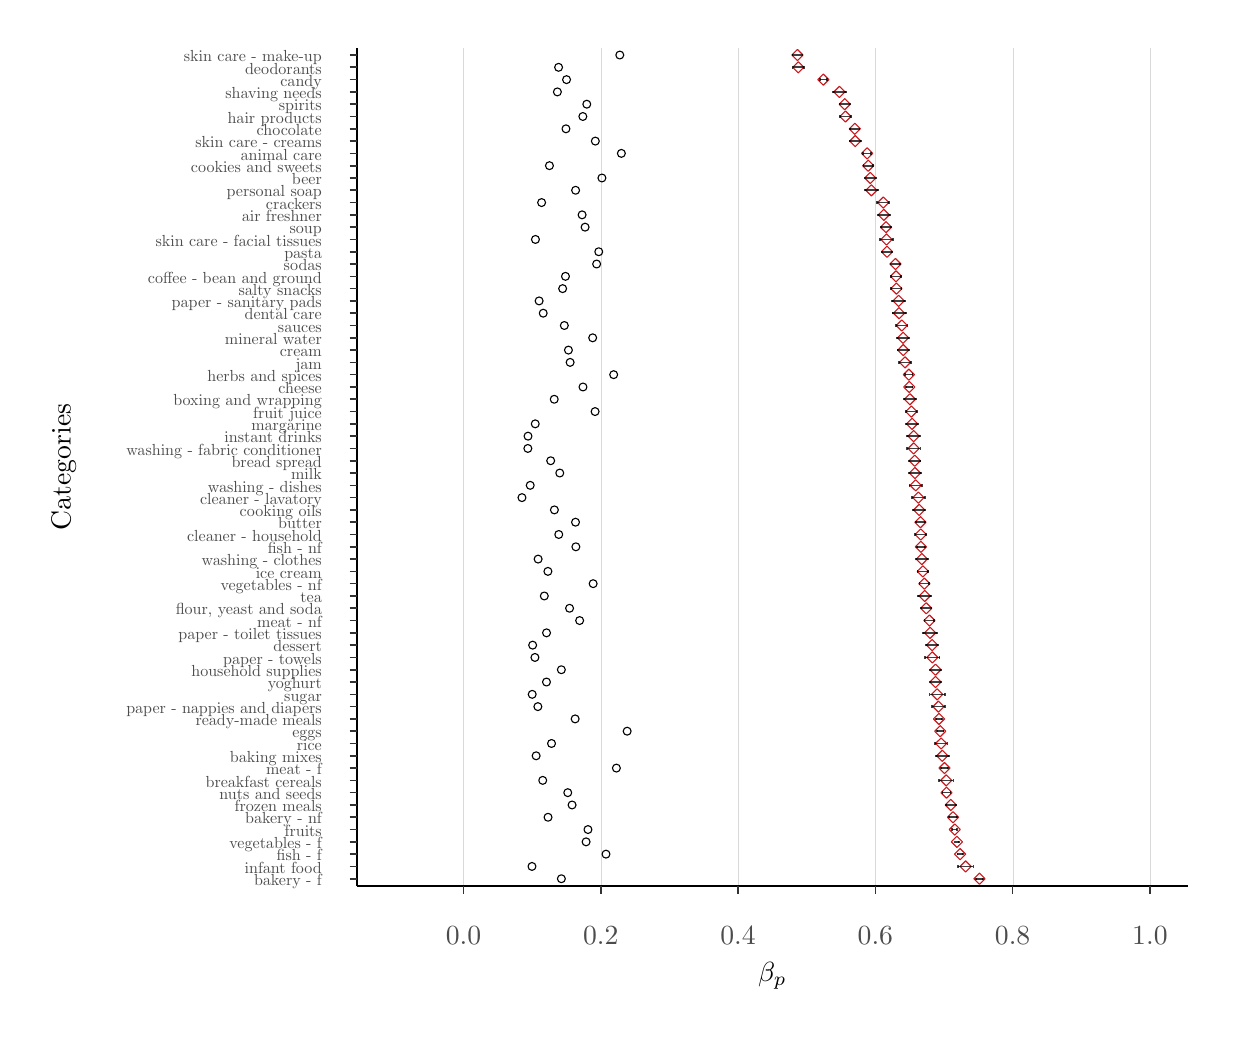
\begin{tikzpicture}[x=1pt,y=1pt]
\definecolor{fillColor}{RGB}{255,255,255}
\path[use as bounding box,fill=fillColor,fill opacity=0.00] (0,0) rectangle (433.62,361.35);
\begin{scope}
\path[clip] (  0.00,  0.00) rectangle (433.62,361.35);
\definecolor{drawColor}{RGB}{255,255,255}
\definecolor{fillColor}{RGB}{255,255,255}

\path[draw=drawColor,line width= 0.6pt,line join=round,line cap=round,fill=fillColor] (  0.00,  0.00) rectangle (433.62,361.35);
\end{scope}
\begin{scope}
\path[clip] (119.04, 51.15) rectangle (419.17,354.12);
\definecolor{drawColor}{RGB}{255,255,255}

\path[draw=drawColor,line width= 0.3pt,line join=round] (132.68, 51.15) --
	(132.68,354.12);

\path[draw=drawColor,line width= 0.3pt,line join=round] (182.29, 51.15) --
	(182.29,354.12);

\path[draw=drawColor,line width= 0.3pt,line join=round] (231.90, 51.15) --
	(231.90,354.12);

\path[draw=drawColor,line width= 0.3pt,line join=round] (281.51, 51.15) --
	(281.51,354.12);

\path[draw=drawColor,line width= 0.3pt,line join=round] (331.11, 51.15) --
	(331.11,354.12);

\path[draw=drawColor,line width= 0.3pt,line join=round] (380.72, 51.15) --
	(380.72,354.12);
\definecolor{drawColor}{gray}{0.85}

\path[draw=drawColor,line width= 0.1pt,line join=round] (157.49, 51.15) --
	(157.49,354.12);

\path[draw=drawColor,line width= 0.1pt,line join=round] (207.09, 51.15) --
	(207.09,354.12);

\path[draw=drawColor,line width= 0.1pt,line join=round] (256.70, 51.15) --
	(256.70,354.12);

\path[draw=drawColor,line width= 0.1pt,line join=round] (306.31, 51.15) --
	(306.31,354.12);

\path[draw=drawColor,line width= 0.1pt,line join=round] (355.92, 51.15) --
	(355.92,354.12);

\path[draw=drawColor,line width= 0.1pt,line join=round] (405.52, 51.15) --
	(405.52,354.12);
\definecolor{drawColor}{RGB}{0,0,0}

\path[draw=drawColor,line width= 0.4pt,line join=round,line cap=round] (200.34,293.71) circle (  1.43);

\path[draw=drawColor,line width= 0.4pt,line join=round,line cap=round] (214.53,315.92) circle (  1.43);

\path[draw=drawColor,line width= 0.4pt,line join=round,line cap=round] (192.85, 53.82) circle (  1.43);

\path[draw=drawColor,line width= 0.4pt,line join=round,line cap=round] (188.03, 76.03) circle (  1.43);

\path[draw=drawColor,line width= 0.4pt,line join=round,line cap=round] (183.73, 98.24) circle (  1.43);

\path[draw=drawColor,line width= 0.4pt,line join=round,line cap=round] (207.50,307.03) circle (  1.43);

\path[draw=drawColor,line width= 0.4pt,line join=round,line cap=round] (190.27,227.07) circle (  1.43);

\path[draw=drawColor,line width= 0.4pt,line join=round,line cap=round] (188.99,204.86) circle (  1.43);

\path[draw=drawColor,line width= 0.4pt,line join=round,line cap=round] (186.11, 89.36) circle (  1.43);

\path[draw=drawColor,line width= 0.4pt,line join=round,line cap=round] (197.96,182.65) circle (  1.43);

\path[draw=drawColor,line width= 0.4pt,line join=round,line cap=round] (194.72,342.57) circle (  1.43);

\path[draw=drawColor,line width= 0.4pt,line join=round,line cap=round] (200.66,231.51) circle (  1.43);

\path[draw=drawColor,line width= 0.4pt,line join=round,line cap=round] (194.51,324.80) circle (  1.43);

\path[draw=drawColor,line width= 0.4pt,line join=round,line cap=round] (191.91,178.21) circle (  1.43);

\path[draw=drawColor,line width= 0.4pt,line join=round,line cap=round] (178.61,191.53) circle (  1.43);

\path[draw=drawColor,line width= 0.4pt,line join=round,line cap=round] (194.33,271.49) circle (  1.43);

\path[draw=drawColor,line width= 0.4pt,line join=round,line cap=round] (188.54,311.48) circle (  1.43);

\path[draw=drawColor,line width= 0.4pt,line join=round,line cap=round] (190.33,187.09) circle (  1.43);

\path[draw=drawColor,line width= 0.4pt,line join=round,line cap=round] (185.71,298.15) circle (  1.43);

\path[draw=drawColor,line width= 0.4pt,line join=round,line cap=round] (195.40,244.84) circle (  1.43);

\path[draw=drawColor,line width= 0.4pt,line join=round,line cap=round] (186.29,258.17) circle (  1.43);

\path[draw=drawColor,line width= 0.4pt,line join=round,line cap=round] (191.84,347.02) circle (  1.43);

\path[draw=drawColor,line width= 0.4pt,line join=round,line cap=round] (182.47,138.22) circle (  1.43);

\path[draw=drawColor,line width= 0.4pt,line join=round,line cap=round] (216.62,107.13) circle (  1.43);

\path[draw=drawColor,line width= 0.4pt,line join=round,line cap=round] (208.97, 62.70) circle (  1.43);

\path[draw=drawColor,line width= 0.4pt,line join=round,line cap=round] (198.09,173.76) circle (  1.43);

\path[draw=drawColor,line width= 0.4pt,line join=round,line cap=round] (195.81,151.55) circle (  1.43);

\path[draw=drawColor,line width= 0.4pt,line join=round,line cap=round] (196.72, 80.47) circle (  1.43);

\path[draw=drawColor,line width= 0.4pt,line join=round,line cap=round] (205.03,222.63) circle (  1.43);

\path[draw=drawColor,line width= 0.4pt,line join=round,line cap=round] (202.46, 71.59) circle (  1.43);

\path[draw=drawColor,line width= 0.4pt,line join=round,line cap=round] (200.61,329.25) circle (  1.43);

\path[draw=drawColor,line width= 0.4pt,line join=round,line cap=round] (211.75,235.96) circle (  1.43);

\path[draw=drawColor,line width= 0.4pt,line join=round,line cap=round] (192.84,129.34) circle (  1.43);

\path[draw=drawColor,line width= 0.4pt,line join=round,line cap=round] (187.99,164.88) circle (  1.43);

\path[draw=drawColor,line width= 0.4pt,line join=round,line cap=round] (182.23, 58.26) circle (  1.43);

\path[draw=drawColor,line width= 0.4pt,line join=round,line cap=round] (180.80,213.74) circle (  1.43);

\path[draw=drawColor,line width= 0.4pt,line join=round,line cap=round] (196.01,240.40) circle (  1.43);

\path[draw=drawColor,line width= 0.4pt,line join=round,line cap=round] (183.41,218.19) circle (  1.43);

\path[draw=drawColor,line width= 0.4pt,line join=round,line cap=round] (212.73, 93.80) circle (  1.43);

\path[draw=drawColor,line width= 0.4pt,line join=round,line cap=round] (199.45,147.11) circle (  1.43);

\path[draw=drawColor,line width= 0.4pt,line join=round,line cap=round] (192.27,200.42) circle (  1.43);

\path[draw=drawColor,line width= 0.4pt,line join=round,line cap=round] (204.16,249.28) circle (  1.43);

\path[draw=drawColor,line width= 0.4pt,line join=round,line cap=round] (195.16, 84.92) circle (  1.43);

\path[draw=drawColor,line width= 0.4pt,line join=round,line cap=round] (184.36,116.01) circle (  1.43);

\path[draw=drawColor,line width= 0.4pt,line join=round,line cap=round] (184.81,262.61) circle (  1.43);

\path[draw=drawColor,line width= 0.4pt,line join=round,line cap=round] (187.49,142.67) circle (  1.43);

\path[draw=drawColor,line width= 0.4pt,line join=round,line cap=round] (183.30,133.78) circle (  1.43);

\path[draw=drawColor,line width= 0.4pt,line join=round,line cap=round] (206.36,280.38) circle (  1.43);

\path[draw=drawColor,line width= 0.4pt,line join=round,line cap=round] (197.99,302.59) circle (  1.43);

\path[draw=drawColor,line width= 0.4pt,line join=round,line cap=round] (197.83,111.57) circle (  1.43);

\path[draw=drawColor,line width= 0.4pt,line join=round,line cap=round] (189.29,102.69) circle (  1.43);

\path[draw=drawColor,line width= 0.4pt,line join=round,line cap=round] (193.31,267.05) circle (  1.43);

\path[draw=drawColor,line width= 0.4pt,line join=round,line cap=round] (193.92,253.73) circle (  1.43);

\path[draw=drawColor,line width= 0.4pt,line join=round,line cap=round] (191.41,338.13) circle (  1.43);

\path[draw=drawColor,line width= 0.4pt,line join=round,line cap=round] (205.12,320.36) circle (  1.43);

\path[draw=drawColor,line width= 0.4pt,line join=round,line cap=round] (183.48,284.82) circle (  1.43);

\path[draw=drawColor,line width= 0.4pt,line join=round,line cap=round] (213.96,351.46) circle (  1.43);

\path[draw=drawColor,line width= 0.4pt,line join=round,line cap=round] (205.59,275.94) circle (  1.43);

\path[draw=drawColor,line width= 0.4pt,line join=round,line cap=round] (201.42,289.26) circle (  1.43);

\path[draw=drawColor,line width= 0.4pt,line join=round,line cap=round] (202.03,333.69) circle (  1.43);

\path[draw=drawColor,line width= 0.4pt,line join=round,line cap=round] (182.31,120.45) circle (  1.43);

\path[draw=drawColor,line width= 0.4pt,line join=round,line cap=round] (186.68,155.99) circle (  1.43);

\path[draw=drawColor,line width= 0.4pt,line join=round,line cap=round] (201.78, 67.15) circle (  1.43);

\path[draw=drawColor,line width= 0.4pt,line join=round,line cap=round] (204.33,160.44) circle (  1.43);

\path[draw=drawColor,line width= 0.4pt,line join=round,line cap=round] (184.45,169.32) circle (  1.43);

\path[draw=drawColor,line width= 0.4pt,line join=round,line cap=round] (181.59,195.97) circle (  1.43);

\path[draw=drawColor,line width= 0.4pt,line join=round,line cap=round] (180.74,209.30) circle (  1.43);

\path[draw=drawColor,line width= 0.4pt,line join=round,line cap=round] (187.47,124.90) circle (  1.43);
\definecolor{drawColor}{RGB}{203,24,29}

\path[draw=drawColor,line width= 0.4pt,line join=round,line cap=round] (307.34,293.71) --
	(309.35,295.72) --
	(311.37,293.71) --
	(309.35,291.69) --
	cycle;

\path[draw=drawColor,line width= 0.4pt,line join=round,line cap=round] (301.33,315.92) --
	(303.34,317.94) --
	(305.36,315.92) --
	(303.34,313.90) --
	cycle;

\path[draw=drawColor,line width= 0.4pt,line join=round,line cap=round] (341.91, 53.82) --
	(343.93, 55.84) --
	(345.95, 53.82) --
	(343.93, 51.80) --
	cycle;

\path[draw=drawColor,line width= 0.4pt,line join=round,line cap=round] (332.35, 76.03) --
	(334.37, 78.05) --
	(336.39, 76.03) --
	(334.37, 74.01) --
	cycle;

\path[draw=drawColor,line width= 0.4pt,line join=round,line cap=round] (328.48, 98.24) --
	(330.50,100.26) --
	(332.51, 98.24) --
	(330.50, 96.23) --
	cycle;

\path[draw=drawColor,line width= 0.4pt,line join=round,line cap=round] (302.47,307.03) --
	(304.48,309.05) --
	(306.50,307.03) --
	(304.48,305.02) --
	cycle;

\path[draw=drawColor,line width= 0.4pt,line join=round,line cap=round] (316.78,227.07) --
	(318.79,229.09) --
	(320.81,227.07) --
	(318.79,225.05) --
	cycle;

\path[draw=drawColor,line width= 0.4pt,line join=round,line cap=round] (318.53,204.86) --
	(320.55,206.88) --
	(322.57,204.86) --
	(320.55,202.84) --
	cycle;

\path[draw=drawColor,line width= 0.4pt,line join=round,line cap=round] (329.88, 89.36) --
	(331.90, 91.38) --
	(333.92, 89.36) --
	(331.90, 87.34) --
	cycle;

\path[draw=drawColor,line width= 0.4pt,line join=round,line cap=round] (320.59,182.65) --
	(322.60,184.67) --
	(324.62,182.65) --
	(322.60,180.63) --
	cycle;

\path[draw=drawColor,line width= 0.4pt,line join=round,line cap=round] (285.48,342.57) --
	(287.50,344.59) --
	(289.51,342.57) --
	(287.50,340.56) --
	cycle;

\path[draw=drawColor,line width= 0.4pt,line join=round,line cap=round] (316.54,231.51) --
	(318.56,233.53) --
	(320.57,231.51) --
	(318.56,229.50) --
	cycle;

\path[draw=drawColor,line width= 0.4pt,line join=round,line cap=round] (296.87,324.80) --
	(298.89,326.82) --
	(300.90,324.80) --
	(298.89,322.79) --
	cycle;

\path[draw=drawColor,line width= 0.4pt,line join=round,line cap=round] (320.70,178.21) --
	(322.72,180.22) --
	(324.74,178.21) --
	(322.72,176.19) --
	cycle;

\path[draw=drawColor,line width= 0.4pt,line join=round,line cap=round] (319.82,191.53) --
	(321.84,193.55) --
	(323.86,191.53) --
	(321.84,189.51) --
	cycle;

\path[draw=drawColor,line width= 0.4pt,line join=round,line cap=round] (311.75,271.49) --
	(313.77,273.51) --
	(315.78,271.49) --
	(313.77,269.48) --
	cycle;

\path[draw=drawColor,line width= 0.4pt,line join=round,line cap=round] (301.71,311.48) --
	(303.73,313.49) --
	(305.75,311.48) --
	(303.73,309.46) --
	cycle;

\path[draw=drawColor,line width= 0.4pt,line join=round,line cap=round] (320.11,187.09) --
	(322.13,189.11) --
	(324.15,187.09) --
	(322.13,185.07) --
	cycle;

\path[draw=drawColor,line width= 0.4pt,line join=round,line cap=round] (307.15,298.15) --
	(309.16,300.17) --
	(311.18,298.15) --
	(309.16,296.13) --
	cycle;

\path[draw=drawColor,line width= 0.4pt,line join=round,line cap=round] (314.38,244.84) --
	(316.39,246.86) --
	(318.41,244.84) --
	(316.39,242.82) --
	cycle;

\path[draw=drawColor,line width= 0.4pt,line join=round,line cap=round] (312.85,258.17) --
	(314.87,260.19) --
	(316.89,258.17) --
	(314.87,256.15) --
	cycle;

\path[draw=drawColor,line width= 0.4pt,line join=round,line cap=round] (276.45,347.02) --
	(278.46,349.03) --
	(280.48,347.02) --
	(278.46,345.00) --
	cycle;

\path[draw=drawColor,line width= 0.4pt,line join=round,line cap=round] (324.80,138.22) --
	(326.82,140.24) --
	(328.84,138.22) --
	(326.82,136.21) --
	cycle;

\path[draw=drawColor,line width= 0.4pt,line join=round,line cap=round] (327.73,107.13) --
	(329.75,109.14) --
	(331.76,107.13) --
	(329.75,105.11) --
	cycle;

\path[draw=drawColor,line width= 0.4pt,line join=round,line cap=round] (334.91, 62.70) --
	(336.92, 64.72) --
	(338.94, 62.70) --
	(336.92, 60.69) --
	cycle;

\path[draw=drawColor,line width= 0.4pt,line join=round,line cap=round] (320.75,173.76) --
	(322.77,175.78) --
	(324.79,173.76) --
	(322.77,171.75) --
	cycle;

\path[draw=drawColor,line width= 0.4pt,line join=round,line cap=round] (322.67,151.55) --
	(324.68,153.57) --
	(326.70,151.55) --
	(324.68,149.53) --
	cycle;

\path[draw=drawColor,line width= 0.4pt,line join=round,line cap=round] (331.55, 80.47) --
	(333.57, 82.49) --
	(335.59, 80.47) --
	(333.57, 78.46) --
	cycle;

\path[draw=drawColor,line width= 0.4pt,line join=round,line cap=round] (317.29,222.63) --
	(319.31,224.65) --
	(321.32,222.63) --
	(319.31,220.61) --
	cycle;

\path[draw=drawColor,line width= 0.4pt,line join=round,line cap=round] (332.98, 71.59) --
	(335.00, 73.61) --
	(337.02, 71.59) --
	(335.00, 69.57) --
	cycle;

\path[draw=drawColor,line width= 0.4pt,line join=round,line cap=round] (293.46,329.25) --
	(295.48,331.26) --
	(297.50,329.25) --
	(295.48,327.23) --
	cycle;

\path[draw=drawColor,line width= 0.4pt,line join=round,line cap=round] (316.40,235.96) --
	(318.42,237.97) --
	(320.43,235.96) --
	(318.42,233.94) --
	cycle;

\path[draw=drawColor,line width= 0.4pt,line join=round,line cap=round] (326.00,129.34) --
	(328.02,131.36) --
	(330.04,129.34) --
	(328.02,127.32) --
	cycle;

\path[draw=drawColor,line width= 0.4pt,line join=round,line cap=round] (321.46,164.88) --
	(323.48,166.90) --
	(325.50,164.88) --
	(323.48,162.86) --
	cycle;

\path[draw=drawColor,line width= 0.4pt,line join=round,line cap=round] (336.91, 58.26) --
	(338.92, 60.28) --
	(340.94, 58.26) --
	(338.92, 56.24) --
	cycle;

\path[draw=drawColor,line width= 0.4pt,line join=round,line cap=round] (318.12,213.74) --
	(320.14,215.76) --
	(322.16,213.74) --
	(320.14,211.73) --
	cycle;

\path[draw=drawColor,line width= 0.4pt,line join=round,line cap=round] (315.01,240.40) --
	(317.03,242.42) --
	(319.05,240.40) --
	(317.03,238.38) --
	cycle;

\path[draw=drawColor,line width= 0.4pt,line join=round,line cap=round] (317.55,218.19) --
	(319.57,220.20) --
	(321.59,218.19) --
	(319.57,216.17) --
	cycle;

\path[draw=drawColor,line width= 0.4pt,line join=round,line cap=round] (329.27, 93.80) --
	(331.29, 95.82) --
	(333.30, 93.80) --
	(331.29, 91.78) --
	cycle;

\path[draw=drawColor,line width= 0.4pt,line join=round,line cap=round] (323.83,147.11) --
	(325.85,149.13) --
	(327.87,147.11) --
	(325.85,145.09) --
	cycle;

\path[draw=drawColor,line width= 0.4pt,line join=round,line cap=round] (318.61,200.42) --
	(320.62,202.43) --
	(322.64,200.42) --
	(320.62,198.40) --
	cycle;

\path[draw=drawColor,line width= 0.4pt,line join=round,line cap=round] (314.30,249.28) --
	(316.32,251.30) --
	(318.33,249.28) --
	(316.32,247.27) --
	cycle;

\path[draw=drawColor,line width= 0.4pt,line join=round,line cap=round] (330.00, 84.92) --
	(332.01, 86.93) --
	(334.03, 84.92) --
	(332.01, 82.90) --
	cycle;

\path[draw=drawColor,line width= 0.4pt,line join=round,line cap=round] (327.10,116.01) --
	(329.12,118.03) --
	(331.13,116.01) --
	(329.12,113.99) --
	cycle;

\path[draw=drawColor,line width= 0.4pt,line join=round,line cap=round] (312.70,262.61) --
	(314.71,264.63) --
	(316.73,262.61) --
	(314.71,260.59) --
	cycle;

\path[draw=drawColor,line width= 0.4pt,line join=round,line cap=round] (324.06,142.67) --
	(326.08,144.68) --
	(328.09,142.67) --
	(326.08,140.65) --
	cycle;

\path[draw=drawColor,line width= 0.4pt,line join=round,line cap=round] (324.89,133.78) --
	(326.90,135.80) --
	(328.92,133.78) --
	(326.90,131.76) --
	cycle;

\path[draw=drawColor,line width= 0.4pt,line join=round,line cap=round] (308.50,280.38) --
	(310.51,282.40) --
	(312.53,280.38) --
	(310.51,278.36) --
	cycle;

\path[draw=drawColor,line width= 0.4pt,line join=round,line cap=round] (302.84,302.59) --
	(304.86,304.61) --
	(306.88,302.59) --
	(304.86,300.57) --
	cycle;

\path[draw=drawColor,line width= 0.4pt,line join=round,line cap=round] (327.29,111.57) --
	(329.31,113.59) --
	(331.33,111.57) --
	(329.31,109.55) --
	cycle;

\path[draw=drawColor,line width= 0.4pt,line join=round,line cap=round] (328.05,102.69) --
	(330.07,104.70) --
	(332.09,102.69) --
	(330.07,100.67) --
	cycle;

\path[draw=drawColor,line width= 0.4pt,line join=round,line cap=round] (311.90,267.05) --
	(313.92,269.07) --
	(315.94,267.05) --
	(313.92,265.04) --
	cycle;

\path[draw=drawColor,line width= 0.4pt,line join=round,line cap=round] (313.85,253.73) --
	(315.87,255.74) --
	(317.89,253.73) --
	(315.87,251.71) --
	cycle;

\path[draw=drawColor,line width= 0.4pt,line join=round,line cap=round] (291.30,338.13) --
	(293.32,340.15) --
	(295.34,338.13) --
	(293.32,336.11) --
	cycle;

\path[draw=drawColor,line width= 0.4pt,line join=round,line cap=round] (297.02,320.36) --
	(299.04,322.38) --
	(301.06,320.36) --
	(299.04,318.34) --
	cycle;

\path[draw=drawColor,line width= 0.4pt,line join=round,line cap=round] (308.31,284.82) --
	(310.33,286.84) --
	(312.35,284.82) --
	(310.33,282.80) --
	cycle;

\path[draw=drawColor,line width= 0.4pt,line join=round,line cap=round] (276.14,351.46) --
	(278.16,353.48) --
	(280.18,351.46) --
	(278.16,349.44) --
	cycle;

\path[draw=drawColor,line width= 0.4pt,line join=round,line cap=round] (311.54,275.94) --
	(313.56,277.95) --
	(315.58,275.94) --
	(313.56,273.92) --
	cycle;

\path[draw=drawColor,line width= 0.4pt,line join=round,line cap=round] (308.14,289.26) --
	(310.16,291.28) --
	(312.18,289.26) --
	(310.16,287.25) --
	cycle;

\path[draw=drawColor,line width= 0.4pt,line join=round,line cap=round] (293.22,333.69) --
	(295.24,335.71) --
	(297.26,333.69) --
	(295.24,331.67) --
	cycle;

\path[draw=drawColor,line width= 0.4pt,line join=round,line cap=round] (326.63,120.45) --
	(328.64,122.47) --
	(330.66,120.45) --
	(328.64,118.44) --
	cycle;

\path[draw=drawColor,line width= 0.4pt,line join=round,line cap=round] (322.12,155.99) --
	(324.14,158.01) --
	(326.16,155.99) --
	(324.14,153.98) --
	cycle;

\path[draw=drawColor,line width= 0.4pt,line join=round,line cap=round] (333.75, 67.15) --
	(335.77, 69.16) --
	(337.78, 67.15) --
	(335.77, 65.13) --
	cycle;

\path[draw=drawColor,line width= 0.4pt,line join=round,line cap=round] (321.99,160.44) --
	(324.01,162.45) --
	(326.02,160.44) --
	(324.01,158.42) --
	cycle;

\path[draw=drawColor,line width= 0.4pt,line join=round,line cap=round] (321.07,169.32) --
	(323.09,171.34) --
	(325.10,169.32) --
	(323.09,167.30) --
	cycle;

\path[draw=drawColor,line width= 0.4pt,line join=round,line cap=round] (318.86,195.97) --
	(320.88,197.99) --
	(322.90,195.97) --
	(320.88,193.96) --
	cycle;

\path[draw=drawColor,line width= 0.4pt,line join=round,line cap=round] (318.13,209.30) --
	(320.14,211.32) --
	(322.16,209.30) --
	(320.14,207.28) --
	cycle;

\path[draw=drawColor,line width= 0.4pt,line join=round,line cap=round] (326.02,124.90) --
	(328.04,126.91) --
	(330.06,124.90) --
	(328.04,122.88) --
	cycle;
\definecolor{drawColor}{RGB}{0,0,0}

\path[draw=drawColor,draw opacity=0.75,line width= 0.6pt,line join=round] (311.53,293.26) --
	(311.53,294.15);

\path[draw=drawColor,draw opacity=0.75,line width= 0.6pt,line join=round] (311.53,293.71) --
	(307.18,293.71);

\path[draw=drawColor,draw opacity=0.75,line width= 0.6pt,line join=round] (307.18,293.26) --
	(307.18,294.15);

\path[draw=drawColor,draw opacity=0.75,line width= 0.6pt,line join=round] (304.83,315.47) --
	(304.83,316.36);

\path[draw=drawColor,draw opacity=0.75,line width= 0.6pt,line join=round] (304.83,315.92) --
	(301.86,315.92);

\path[draw=drawColor,draw opacity=0.75,line width= 0.6pt,line join=round] (301.86,315.47) --
	(301.86,316.36);

\path[draw=drawColor,draw opacity=0.75,line width= 0.6pt,line join=round] (345.18, 53.37) --
	(345.18, 54.26);

\path[draw=drawColor,draw opacity=0.75,line width= 0.6pt,line join=round] (345.18, 53.82) --
	(342.67, 53.82);

\path[draw=drawColor,draw opacity=0.75,line width= 0.6pt,line join=round] (342.67, 53.37) --
	(342.67, 54.26);

\path[draw=drawColor,draw opacity=0.75,line width= 0.6pt,line join=round] (335.76, 75.59) --
	(335.76, 76.48);

\path[draw=drawColor,draw opacity=0.75,line width= 0.6pt,line join=round] (335.76, 76.03) --
	(332.98, 76.03);

\path[draw=drawColor,draw opacity=0.75,line width= 0.6pt,line join=round] (332.98, 75.59) --
	(332.98, 76.48);

\path[draw=drawColor,draw opacity=0.75,line width= 0.6pt,line join=round] (332.89, 97.80) --
	(332.89, 98.69);

\path[draw=drawColor,draw opacity=0.75,line width= 0.6pt,line join=round] (332.89, 98.24) --
	(328.10, 98.24);

\path[draw=drawColor,draw opacity=0.75,line width= 0.6pt,line join=round] (328.10, 97.80) --
	(328.10, 98.69);

\path[draw=drawColor,draw opacity=0.75,line width= 0.6pt,line join=round] (306.53,306.59) --
	(306.53,307.48);

\path[draw=drawColor,draw opacity=0.75,line width= 0.6pt,line join=round] (306.53,307.03) --
	(302.44,307.03);

\path[draw=drawColor,draw opacity=0.75,line width= 0.6pt,line join=round] (302.44,306.59) --
	(302.44,307.48);

\path[draw=drawColor,draw opacity=0.75,line width= 0.6pt,line join=round] (320.98,226.63) --
	(320.98,227.52);

\path[draw=drawColor,draw opacity=0.75,line width= 0.6pt,line join=round] (320.98,227.07) --
	(316.61,227.07);

\path[draw=drawColor,draw opacity=0.75,line width= 0.6pt,line join=round] (316.61,226.63) --
	(316.61,227.52);

\path[draw=drawColor,draw opacity=0.75,line width= 0.6pt,line join=round] (322.67,204.42) --
	(322.67,205.30);

\path[draw=drawColor,draw opacity=0.75,line width= 0.6pt,line join=round] (322.67,204.86) --
	(318.42,204.86);

\path[draw=drawColor,draw opacity=0.75,line width= 0.6pt,line join=round] (318.42,204.42) --
	(318.42,205.30);

\path[draw=drawColor,draw opacity=0.75,line width= 0.6pt,line join=round] (334.49, 88.91) --
	(334.49, 89.80);

\path[draw=drawColor,draw opacity=0.75,line width= 0.6pt,line join=round] (334.49, 89.36) --
	(329.31, 89.36);

\path[draw=drawColor,draw opacity=0.75,line width= 0.6pt,line join=round] (329.31, 88.91) --
	(329.31, 89.80);

\path[draw=drawColor,draw opacity=0.75,line width= 0.6pt,line join=round] (324.30,182.20) --
	(324.30,183.09);

\path[draw=drawColor,draw opacity=0.75,line width= 0.6pt,line join=round] (324.30,182.65) --
	(320.91,182.65);

\path[draw=drawColor,draw opacity=0.75,line width= 0.6pt,line join=round] (320.91,182.20) --
	(320.91,183.09);

\path[draw=drawColor,draw opacity=0.75,line width= 0.6pt,line join=round] (288.76,342.13) --
	(288.76,343.02);

\path[draw=drawColor,draw opacity=0.75,line width= 0.6pt,line join=round] (288.76,342.57) --
	(286.23,342.57);

\path[draw=drawColor,draw opacity=0.75,line width= 0.6pt,line join=round] (286.23,342.13) --
	(286.23,343.02);

\path[draw=drawColor,draw opacity=0.75,line width= 0.6pt,line join=round] (319.76,231.07) --
	(319.76,231.96);

\path[draw=drawColor,draw opacity=0.75,line width= 0.6pt,line join=round] (319.76,231.51) --
	(317.36,231.51);

\path[draw=drawColor,draw opacity=0.75,line width= 0.6pt,line join=round] (317.36,231.07) --
	(317.36,231.96);

\path[draw=drawColor,draw opacity=0.75,line width= 0.6pt,line join=round] (300.59,324.36) --
	(300.59,325.25);

\path[draw=drawColor,draw opacity=0.75,line width= 0.6pt,line join=round] (300.59,324.80) --
	(297.19,324.80);

\path[draw=drawColor,draw opacity=0.75,line width= 0.6pt,line join=round] (297.19,324.36) --
	(297.19,325.25);

\path[draw=drawColor,draw opacity=0.75,line width= 0.6pt,line join=round] (324.71,177.76) --
	(324.71,178.65);

\path[draw=drawColor,draw opacity=0.75,line width= 0.6pt,line join=round] (324.71,178.21) --
	(320.73,178.21);

\path[draw=drawColor,draw opacity=0.75,line width= 0.6pt,line join=round] (320.73,177.76) --
	(320.73,178.65);

\path[draw=drawColor,draw opacity=0.75,line width= 0.6pt,line join=round] (324.23,191.09) --
	(324.23,191.98);

\path[draw=drawColor,draw opacity=0.75,line width= 0.6pt,line join=round] (324.23,191.53) --
	(319.45,191.53);

\path[draw=drawColor,draw opacity=0.75,line width= 0.6pt,line join=round] (319.45,191.09) --
	(319.45,191.98);

\path[draw=drawColor,draw opacity=0.75,line width= 0.6pt,line join=round] (315.63,271.05) --
	(315.63,271.94);

\path[draw=drawColor,draw opacity=0.75,line width= 0.6pt,line join=round] (315.63,271.49) --
	(311.90,271.49);

\path[draw=drawColor,draw opacity=0.75,line width= 0.6pt,line join=round] (311.90,271.05) --
	(311.90,271.94);

\path[draw=drawColor,draw opacity=0.75,line width= 0.6pt,line join=round] (305.45,311.03) --
	(305.45,311.92);

\path[draw=drawColor,draw opacity=0.75,line width= 0.6pt,line join=round] (305.45,311.48) --
	(302.01,311.48);

\path[draw=drawColor,draw opacity=0.75,line width= 0.6pt,line join=round] (302.01,311.03) --
	(302.01,311.92);

\path[draw=drawColor,draw opacity=0.75,line width= 0.6pt,line join=round] (324.26,186.65) --
	(324.26,187.53);

\path[draw=drawColor,draw opacity=0.75,line width= 0.6pt,line join=round] (324.26,187.09) --
	(320.00,187.09);

\path[draw=drawColor,draw opacity=0.75,line width= 0.6pt,line join=round] (320.00,186.65) --
	(320.00,187.53);

\path[draw=drawColor,draw opacity=0.75,line width= 0.6pt,line join=round] (311.35,297.70) --
	(311.35,298.59);

\path[draw=drawColor,draw opacity=0.75,line width= 0.6pt,line join=round] (311.35,298.15) --
	(306.98,298.15);

\path[draw=drawColor,draw opacity=0.75,line width= 0.6pt,line join=round] (306.98,297.70) --
	(306.98,298.59);

\path[draw=drawColor,draw opacity=0.75,line width= 0.6pt,line join=round] (318.50,244.40) --
	(318.50,245.29);

\path[draw=drawColor,draw opacity=0.75,line width= 0.6pt,line join=round] (318.50,244.84) --
	(314.29,244.84);

\path[draw=drawColor,draw opacity=0.75,line width= 0.6pt,line join=round] (314.29,244.40) --
	(314.29,245.29);

\path[draw=drawColor,draw opacity=0.75,line width= 0.6pt,line join=round] (317.29,257.72) --
	(317.29,258.61);

\path[draw=drawColor,draw opacity=0.75,line width= 0.6pt,line join=round] (317.29,258.17) --
	(312.45,258.17);

\path[draw=drawColor,draw opacity=0.75,line width= 0.6pt,line join=round] (312.45,257.72) --
	(312.45,258.61);

\path[draw=drawColor,draw opacity=0.75,line width= 0.6pt,line join=round] (280.52,346.57) --
	(280.52,347.46);

\path[draw=drawColor,draw opacity=0.75,line width= 0.6pt,line join=round] (280.52,347.02) --
	(276.41,347.02);

\path[draw=drawColor,draw opacity=0.75,line width= 0.6pt,line join=round] (276.41,346.57) --
	(276.41,347.46);

\path[draw=drawColor,draw opacity=0.75,line width= 0.6pt,line join=round] (329.04,137.78) --
	(329.04,138.67);

\path[draw=drawColor,draw opacity=0.75,line width= 0.6pt,line join=round] (329.04,138.22) --
	(324.60,138.22);

\path[draw=drawColor,draw opacity=0.75,line width= 0.6pt,line join=round] (324.60,137.78) --
	(324.60,138.67);

\path[draw=drawColor,draw opacity=0.75,line width= 0.6pt,line join=round] (330.95,106.68) --
	(330.95,107.57);

\path[draw=drawColor,draw opacity=0.75,line width= 0.6pt,line join=round] (330.95,107.13) --
	(328.54,107.13);

\path[draw=drawColor,draw opacity=0.75,line width= 0.6pt,line join=round] (328.54,106.68) --
	(328.54,107.57);

\path[draw=drawColor,draw opacity=0.75,line width= 0.6pt,line join=round] (337.91, 62.26) --
	(337.91, 63.15);

\path[draw=drawColor,draw opacity=0.75,line width= 0.6pt,line join=round] (337.91, 62.70) --
	(335.94, 62.70);

\path[draw=drawColor,draw opacity=0.75,line width= 0.6pt,line join=round] (335.94, 62.26) --
	(335.94, 63.15);

\path[draw=drawColor,draw opacity=0.75,line width= 0.6pt,line join=round] (324.30,173.32) --
	(324.30,174.21);

\path[draw=drawColor,draw opacity=0.75,line width= 0.6pt,line join=round] (324.30,173.76) --
	(321.24,173.76);

\path[draw=drawColor,draw opacity=0.75,line width= 0.6pt,line join=round] (321.24,173.32) --
	(321.24,174.21);

\path[draw=drawColor,draw opacity=0.75,line width= 0.6pt,line join=round] (326.65,151.11) --
	(326.65,152.00);

\path[draw=drawColor,draw opacity=0.75,line width= 0.6pt,line join=round] (326.65,151.55) --
	(322.72,151.55);

\path[draw=drawColor,draw opacity=0.75,line width= 0.6pt,line join=round] (322.72,151.11) --
	(322.72,152.00);

\path[draw=drawColor,draw opacity=0.75,line width= 0.6pt,line join=round] (335.38, 80.03) --
	(335.38, 80.92);

\path[draw=drawColor,draw opacity=0.75,line width= 0.6pt,line join=round] (335.38, 80.47) --
	(331.76, 80.47);

\path[draw=drawColor,draw opacity=0.75,line width= 0.6pt,line join=round] (331.76, 80.03) --
	(331.76, 80.92);

\path[draw=drawColor,draw opacity=0.75,line width= 0.6pt,line join=round] (321.31,222.18) --
	(321.31,223.07);

\path[draw=drawColor,draw opacity=0.75,line width= 0.6pt,line join=round] (321.31,222.63) --
	(317.30,222.63);

\path[draw=drawColor,draw opacity=0.75,line width= 0.6pt,line join=round] (317.30,222.18) --
	(317.30,223.07);

\path[draw=drawColor,draw opacity=0.75,line width= 0.6pt,line join=round] (335.89, 71.14) --
	(335.89, 72.03);

\path[draw=drawColor,draw opacity=0.75,line width= 0.6pt,line join=round] (335.89, 71.59) --
	(334.11, 71.59);

\path[draw=drawColor,draw opacity=0.75,line width= 0.6pt,line join=round] (334.11, 71.14) --
	(334.11, 72.03);

\path[draw=drawColor,draw opacity=0.75,line width= 0.6pt,line join=round] (297.49,328.80) --
	(297.49,329.69);

\path[draw=drawColor,draw opacity=0.75,line width= 0.6pt,line join=round] (297.49,329.25) --
	(293.47,329.25);

\path[draw=drawColor,draw opacity=0.75,line width= 0.6pt,line join=round] (293.47,328.80) --
	(293.47,329.69);

\path[draw=drawColor,draw opacity=0.75,line width= 0.6pt,line join=round] (319.74,235.51) --
	(319.74,236.40);

\path[draw=drawColor,draw opacity=0.75,line width= 0.6pt,line join=round] (319.74,235.96) --
	(317.09,235.96);

\path[draw=drawColor,draw opacity=0.75,line width= 0.6pt,line join=round] (317.09,235.51) --
	(317.09,236.40);

\path[draw=drawColor,draw opacity=0.75,line width= 0.6pt,line join=round] (330.02,128.90) --
	(330.02,129.78);

\path[draw=drawColor,draw opacity=0.75,line width= 0.6pt,line join=round] (330.02,129.34) --
	(326.02,129.34);

\path[draw=drawColor,draw opacity=0.75,line width= 0.6pt,line join=round] (326.02,128.90) --
	(326.02,129.78);

\path[draw=drawColor,draw opacity=0.75,line width= 0.6pt,line join=round] (325.43,164.43) --
	(325.43,165.32);

\path[draw=drawColor,draw opacity=0.75,line width= 0.6pt,line join=round] (325.43,164.88) --
	(321.53,164.88);

\path[draw=drawColor,draw opacity=0.75,line width= 0.6pt,line join=round] (321.53,164.43) --
	(321.53,165.32);

\path[draw=drawColor,draw opacity=0.75,line width= 0.6pt,line join=round] (341.73, 57.82) --
	(341.73, 58.71);

\path[draw=drawColor,draw opacity=0.75,line width= 0.6pt,line join=round] (341.73, 58.26) --
	(336.11, 58.26);

\path[draw=drawColor,draw opacity=0.75,line width= 0.6pt,line join=round] (336.11, 57.82) --
	(336.11, 58.71);

\path[draw=drawColor,draw opacity=0.75,line width= 0.6pt,line join=round] (322.52,213.30) --
	(322.52,214.19);

\path[draw=drawColor,draw opacity=0.75,line width= 0.6pt,line join=round] (322.52,213.74) --
	(317.76,213.74);

\path[draw=drawColor,draw opacity=0.75,line width= 0.6pt,line join=round] (317.76,213.30) --
	(317.76,214.19);

\path[draw=drawColor,draw opacity=0.75,line width= 0.6pt,line join=round] (319.10,239.95) --
	(319.10,240.84);

\path[draw=drawColor,draw opacity=0.75,line width= 0.6pt,line join=round] (319.10,240.40) --
	(314.96,240.40);

\path[draw=drawColor,draw opacity=0.75,line width= 0.6pt,line join=round] (314.96,239.95) --
	(314.96,240.84);

\path[draw=drawColor,draw opacity=0.75,line width= 0.6pt,line join=round] (321.65,217.74) --
	(321.65,218.63);

\path[draw=drawColor,draw opacity=0.75,line width= 0.6pt,line join=round] (321.65,218.19) --
	(317.49,218.19);

\path[draw=drawColor,draw opacity=0.75,line width= 0.6pt,line join=round] (317.49,217.74) --
	(317.49,218.63);

\path[draw=drawColor,draw opacity=0.75,line width= 0.6pt,line join=round] (332.50, 93.36) --
	(332.50, 94.24);

\path[draw=drawColor,draw opacity=0.75,line width= 0.6pt,line join=round] (332.50, 93.80) --
	(330.08, 93.80);

\path[draw=drawColor,draw opacity=0.75,line width= 0.6pt,line join=round] (330.08, 93.36) --
	(330.08, 94.24);

\path[draw=drawColor,draw opacity=0.75,line width= 0.6pt,line join=round] (327.58,146.66) --
	(327.58,147.55);

\path[draw=drawColor,draw opacity=0.75,line width= 0.6pt,line join=round] (327.58,147.11) --
	(324.11,147.11);

\path[draw=drawColor,draw opacity=0.75,line width= 0.6pt,line join=round] (324.11,146.66) --
	(324.11,147.55);

\path[draw=drawColor,draw opacity=0.75,line width= 0.6pt,line join=round] (322.69,199.97) --
	(322.69,200.86);

\path[draw=drawColor,draw opacity=0.75,line width= 0.6pt,line join=round] (322.69,200.42) --
	(318.56,200.42);

\path[draw=drawColor,draw opacity=0.75,line width= 0.6pt,line join=round] (318.56,199.97) --
	(318.56,200.86);

\path[draw=drawColor,draw opacity=0.75,line width= 0.6pt,line join=round] (318.45,248.84) --
	(318.45,249.73);

\path[draw=drawColor,draw opacity=0.75,line width= 0.6pt,line join=round] (318.45,249.28) --
	(314.18,249.28);

\path[draw=drawColor,draw opacity=0.75,line width= 0.6pt,line join=round] (314.18,248.84) --
	(314.18,249.73);

\path[draw=drawColor,draw opacity=0.75,line width= 0.6pt,line join=round] (333.47, 84.47) --
	(333.47, 85.36);

\path[draw=drawColor,draw opacity=0.75,line width= 0.6pt,line join=round] (333.47, 84.92) --
	(330.56, 84.92);

\path[draw=drawColor,draw opacity=0.75,line width= 0.6pt,line join=round] (330.56, 84.47) --
	(330.56, 85.36);

\path[draw=drawColor,draw opacity=0.75,line width= 0.6pt,line join=round] (331.40,115.57) --
	(331.40,116.46);

\path[draw=drawColor,draw opacity=0.75,line width= 0.6pt,line join=round] (331.40,116.01) --
	(326.83,116.01);

\path[draw=drawColor,draw opacity=0.75,line width= 0.6pt,line join=round] (326.83,115.57) --
	(326.83,116.46);

\path[draw=drawColor,draw opacity=0.75,line width= 0.6pt,line join=round] (317.07,262.17) --
	(317.07,263.05);

\path[draw=drawColor,draw opacity=0.75,line width= 0.6pt,line join=round] (317.07,262.61) --
	(312.36,262.61);

\path[draw=drawColor,draw opacity=0.75,line width= 0.6pt,line join=round] (312.36,262.17) --
	(312.36,263.05);

\path[draw=drawColor,draw opacity=0.75,line width= 0.6pt,line join=round] (328.54,142.22) --
	(328.54,143.11);

\path[draw=drawColor,draw opacity=0.75,line width= 0.6pt,line join=round] (328.54,142.67) --
	(323.61,142.67);

\path[draw=drawColor,draw opacity=0.75,line width= 0.6pt,line join=round] (323.61,142.22) --
	(323.61,143.11);

\path[draw=drawColor,draw opacity=0.75,line width= 0.6pt,line join=round] (329.51,133.34) --
	(329.51,134.23);

\path[draw=drawColor,draw opacity=0.75,line width= 0.6pt,line join=round] (329.51,133.78) --
	(324.30,133.78);

\path[draw=drawColor,draw opacity=0.75,line width= 0.6pt,line join=round] (324.30,133.34) --
	(324.30,134.23);

\path[draw=drawColor,draw opacity=0.75,line width= 0.6pt,line join=round] (312.41,279.94) --
	(312.41,280.82);

\path[draw=drawColor,draw opacity=0.75,line width= 0.6pt,line join=round] (312.41,280.38) --
	(308.61,280.38);

\path[draw=drawColor,draw opacity=0.75,line width= 0.6pt,line join=round] (308.61,279.94) --
	(308.61,280.82);

\path[draw=drawColor,draw opacity=0.75,line width= 0.6pt,line join=round] (307.19,302.15) --
	(307.19,303.04);

\path[draw=drawColor,draw opacity=0.75,line width= 0.6pt,line join=round] (307.19,302.59) --
	(302.53,302.59);

\path[draw=drawColor,draw opacity=0.75,line width= 0.6pt,line join=round] (302.53,302.15) --
	(302.53,303.04);

\path[draw=drawColor,draw opacity=0.75,line width= 0.6pt,line join=round] (330.34,111.13) --
	(330.34,112.01);

\path[draw=drawColor,draw opacity=0.75,line width= 0.6pt,line join=round] (330.34,111.57) --
	(328.28,111.57);

\path[draw=drawColor,draw opacity=0.75,line width= 0.6pt,line join=round] (328.28,111.13) --
	(328.28,112.01);

\path[draw=drawColor,draw opacity=0.75,line width= 0.6pt,line join=round] (332.32,102.24) --
	(332.32,103.13);

\path[draw=drawColor,draw opacity=0.75,line width= 0.6pt,line join=round] (332.32,102.69) --
	(327.82,102.69);

\path[draw=drawColor,draw opacity=0.75,line width= 0.6pt,line join=round] (327.82,102.24) --
	(327.82,103.13);

\path[draw=drawColor,draw opacity=0.75,line width= 0.6pt,line join=round] (315.81,266.61) --
	(315.81,267.50);

\path[draw=drawColor,draw opacity=0.75,line width= 0.6pt,line join=round] (315.81,267.05) --
	(312.03,267.05);

\path[draw=drawColor,draw opacity=0.75,line width= 0.6pt,line join=round] (312.03,266.61) --
	(312.03,267.50);

\path[draw=drawColor,draw opacity=0.75,line width= 0.6pt,line join=round] (317.86,253.28) --
	(317.86,254.17);

\path[draw=drawColor,draw opacity=0.75,line width= 0.6pt,line join=round] (317.86,253.73) --
	(313.88,253.73);

\path[draw=drawColor,draw opacity=0.75,line width= 0.6pt,line join=round] (313.88,253.28) --
	(313.88,254.17);

\path[draw=drawColor,draw opacity=0.75,line width= 0.6pt,line join=round] (295.61,337.69) --
	(295.61,338.57);

\path[draw=drawColor,draw opacity=0.75,line width= 0.6pt,line join=round] (295.61,338.13) --
	(291.03,338.13);

\path[draw=drawColor,draw opacity=0.75,line width= 0.6pt,line join=round] (291.03,337.69) --
	(291.03,338.57);

\path[draw=drawColor,draw opacity=0.75,line width= 0.6pt,line join=round] (301.15,319.92) --
	(301.15,320.81);

\path[draw=drawColor,draw opacity=0.75,line width= 0.6pt,line join=round] (301.15,320.36) --
	(296.93,320.36);

\path[draw=drawColor,draw opacity=0.75,line width= 0.6pt,line join=round] (296.93,319.92) --
	(296.93,320.81);

\path[draw=drawColor,draw opacity=0.75,line width= 0.6pt,line join=round] (312.73,284.38) --
	(312.73,285.27);

\path[draw=drawColor,draw opacity=0.75,line width= 0.6pt,line join=round] (312.73,284.82) --
	(307.93,284.82);

\path[draw=drawColor,draw opacity=0.75,line width= 0.6pt,line join=round] (307.93,284.38) --
	(307.93,285.27);

\path[draw=drawColor,draw opacity=0.75,line width= 0.6pt,line join=round] (279.96,351.01) --
	(279.96,351.90);

\path[draw=drawColor,draw opacity=0.75,line width= 0.6pt,line join=round] (279.96,351.46) --
	(276.36,351.46);

\path[draw=drawColor,draw opacity=0.75,line width= 0.6pt,line join=round] (276.36,351.01) --
	(276.36,351.90);

\path[draw=drawColor,draw opacity=0.75,line width= 0.6pt,line join=round] (315.31,275.49) --
	(315.31,276.38);

\path[draw=drawColor,draw opacity=0.75,line width= 0.6pt,line join=round] (315.31,275.94) --
	(311.81,275.94);

\path[draw=drawColor,draw opacity=0.75,line width= 0.6pt,line join=round] (311.81,275.49) --
	(311.81,276.38);

\path[draw=drawColor,draw opacity=0.75,line width= 0.6pt,line join=round] (311.88,288.82) --
	(311.88,289.71);

\path[draw=drawColor,draw opacity=0.75,line width= 0.6pt,line join=round] (311.88,289.26) --
	(308.44,289.26);

\path[draw=drawColor,draw opacity=0.75,line width= 0.6pt,line join=round] (308.44,288.82) --
	(308.44,289.71);

\path[draw=drawColor,draw opacity=0.75,line width= 0.6pt,line join=round] (297.17,333.24) --
	(297.17,334.13);

\path[draw=drawColor,draw opacity=0.75,line width= 0.6pt,line join=round] (297.17,333.69) --
	(293.31,333.69);

\path[draw=drawColor,draw opacity=0.75,line width= 0.6pt,line join=round] (293.31,333.24) --
	(293.31,334.13);

\path[draw=drawColor,draw opacity=0.75,line width= 0.6pt,line join=round] (331.37,120.01) --
	(331.37,120.90);

\path[draw=drawColor,draw opacity=0.75,line width= 0.6pt,line join=round] (331.37,120.45) --
	(325.92,120.45);

\path[draw=drawColor,draw opacity=0.75,line width= 0.6pt,line join=round] (325.92,120.01) --
	(325.92,120.90);

\path[draw=drawColor,draw opacity=0.75,line width= 0.6pt,line join=round] (326.45,155.55) --
	(326.45,156.44);

\path[draw=drawColor,draw opacity=0.75,line width= 0.6pt,line join=round] (326.45,155.99) --
	(321.83,155.99);

\path[draw=drawColor,draw opacity=0.75,line width= 0.6pt,line join=round] (321.83,155.55) --
	(321.83,156.44);

\path[draw=drawColor,draw opacity=0.75,line width= 0.6pt,line join=round] (336.59, 66.70) --
	(336.59, 67.59);

\path[draw=drawColor,draw opacity=0.75,line width= 0.6pt,line join=round] (336.59, 67.15) --
	(334.94, 67.15);

\path[draw=drawColor,draw opacity=0.75,line width= 0.6pt,line join=round] (334.94, 66.70) --
	(334.94, 67.59);

\path[draw=drawColor,draw opacity=0.75,line width= 0.6pt,line join=round] (325.71,159.99) --
	(325.71,160.88);

\path[draw=drawColor,draw opacity=0.75,line width= 0.6pt,line join=round] (325.71,160.44) --
	(322.30,160.44);

\path[draw=drawColor,draw opacity=0.75,line width= 0.6pt,line join=round] (322.30,159.99) --
	(322.30,160.88);

\path[draw=drawColor,draw opacity=0.75,line width= 0.6pt,line join=round] (325.29,168.88) --
	(325.29,169.76);

\path[draw=drawColor,draw opacity=0.75,line width= 0.6pt,line join=round] (325.29,169.32) --
	(320.88,169.32);

\path[draw=drawColor,draw opacity=0.75,line width= 0.6pt,line join=round] (320.88,168.88) --
	(320.88,169.76);

\path[draw=drawColor,draw opacity=0.75,line width= 0.6pt,line join=round] (323.16,195.53) --
	(323.16,196.42);

\path[draw=drawColor,draw opacity=0.75,line width= 0.6pt,line join=round] (323.16,195.97) --
	(318.60,195.97);

\path[draw=drawColor,draw opacity=0.75,line width= 0.6pt,line join=round] (318.60,195.53) --
	(318.60,196.42);

\path[draw=drawColor,draw opacity=0.75,line width= 0.6pt,line join=round] (322.56,208.86) --
	(322.56,209.75);

\path[draw=drawColor,draw opacity=0.75,line width= 0.6pt,line join=round] (322.56,209.30) --
	(317.73,209.30);

\path[draw=drawColor,draw opacity=0.75,line width= 0.6pt,line join=round] (317.73,208.86) --
	(317.73,209.75);

\path[draw=drawColor,draw opacity=0.75,line width= 0.6pt,line join=round] (330.14,124.45) --
	(330.14,125.34);

\path[draw=drawColor,draw opacity=0.75,line width= 0.6pt,line join=round] (330.14,124.90) --
	(325.94,124.90);

\path[draw=drawColor,draw opacity=0.75,line width= 0.6pt,line join=round] (325.94,124.45) --
	(325.94,125.34);
\end{scope}
\begin{scope}
\path[clip] (  0.00,  0.00) rectangle (433.62,361.35);
\definecolor{drawColor}{RGB}{0,0,0}

\path[draw=drawColor,line width= 0.6pt,line join=round] (119.04, 51.15) --
	(119.04,354.12);
\end{scope}
\begin{scope}
\path[clip] (  0.00,  0.00) rectangle (433.62,361.35);
\definecolor{drawColor}{gray}{0.30}

\node[text=drawColor,anchor=base east,inner sep=0pt, outer sep=0pt, scale=  0.58] at (106.29, 51.41) {bakery - f};

\node[text=drawColor,anchor=base east,inner sep=0pt, outer sep=0pt, scale=  0.58] at (106.29, 55.85) {infant food};

\node[text=drawColor,anchor=base east,inner sep=0pt, outer sep=0pt, scale=  0.58] at (106.29, 60.29) {fish - f};

\node[text=drawColor,anchor=base east,inner sep=0pt, outer sep=0pt, scale=  0.58] at (106.29, 64.74) {vegetables - f};

\node[text=drawColor,anchor=base east,inner sep=0pt, outer sep=0pt, scale=  0.58] at (106.29, 69.18) {fruits};

\node[text=drawColor,anchor=base east,inner sep=0pt, outer sep=0pt, scale=  0.58] at (106.29, 73.62) {bakery - nf};

\node[text=drawColor,anchor=base east,inner sep=0pt, outer sep=0pt, scale=  0.58] at (106.29, 78.06) {frozen meals};

\node[text=drawColor,anchor=base east,inner sep=0pt, outer sep=0pt, scale=  0.58] at (106.29, 82.50) {nuts and seeds};

\node[text=drawColor,anchor=base east,inner sep=0pt, outer sep=0pt, scale=  0.58] at (106.29, 86.95) {breakfast cereals};

\node[text=drawColor,anchor=base east,inner sep=0pt, outer sep=0pt, scale=  0.58] at (106.29, 91.39) {meat - f};

\node[text=drawColor,anchor=base east,inner sep=0pt, outer sep=0pt, scale=  0.58] at (106.29, 95.83) {baking mixes};

\node[text=drawColor,anchor=base east,inner sep=0pt, outer sep=0pt, scale=  0.58] at (106.29,100.27) {rice};

\node[text=drawColor,anchor=base east,inner sep=0pt, outer sep=0pt, scale=  0.58] at (106.29,104.72) {eggs};

\node[text=drawColor,anchor=base east,inner sep=0pt, outer sep=0pt, scale=  0.58] at (106.29,109.16) {ready-made meals};

\node[text=drawColor,anchor=base east,inner sep=0pt, outer sep=0pt, scale=  0.58] at (106.29,113.60) {paper - nappies and diapers};

\node[text=drawColor,anchor=base east,inner sep=0pt, outer sep=0pt, scale=  0.58] at (106.29,118.04) {sugar};

\node[text=drawColor,anchor=base east,inner sep=0pt, outer sep=0pt, scale=  0.58] at (106.29,122.49) {yoghurt};

\node[text=drawColor,anchor=base east,inner sep=0pt, outer sep=0pt, scale=  0.58] at (106.29,126.93) {household supplies};

\node[text=drawColor,anchor=base east,inner sep=0pt, outer sep=0pt, scale=  0.58] at (106.29,131.37) {paper - towels};

\node[text=drawColor,anchor=base east,inner sep=0pt, outer sep=0pt, scale=  0.58] at (106.29,135.81) {dessert};

\node[text=drawColor,anchor=base east,inner sep=0pt, outer sep=0pt, scale=  0.58] at (106.29,140.26) {paper - toilet tissues};

\node[text=drawColor,anchor=base east,inner sep=0pt, outer sep=0pt, scale=  0.58] at (106.29,144.70) {meat - nf};

\node[text=drawColor,anchor=base east,inner sep=0pt, outer sep=0pt, scale=  0.58] at (106.29,149.14) {flour, yeast and soda};

\node[text=drawColor,anchor=base east,inner sep=0pt, outer sep=0pt, scale=  0.58] at (106.29,153.58) {tea};

\node[text=drawColor,anchor=base east,inner sep=0pt, outer sep=0pt, scale=  0.58] at (106.29,158.02) {vegetables - nf};

\node[text=drawColor,anchor=base east,inner sep=0pt, outer sep=0pt, scale=  0.58] at (106.29,162.47) {ice cream};

\node[text=drawColor,anchor=base east,inner sep=0pt, outer sep=0pt, scale=  0.58] at (106.29,166.91) {washing - clothes};

\node[text=drawColor,anchor=base east,inner sep=0pt, outer sep=0pt, scale=  0.58] at (106.29,171.35) {fish - nf};

\node[text=drawColor,anchor=base east,inner sep=0pt, outer sep=0pt, scale=  0.58] at (106.29,175.79) {cleaner - household};

\node[text=drawColor,anchor=base east,inner sep=0pt, outer sep=0pt, scale=  0.58] at (106.29,180.24) {butter};

\node[text=drawColor,anchor=base east,inner sep=0pt, outer sep=0pt, scale=  0.58] at (106.29,184.68) {cooking oils};

\node[text=drawColor,anchor=base east,inner sep=0pt, outer sep=0pt, scale=  0.58] at (106.29,189.12) {cleaner - lavatory};

\node[text=drawColor,anchor=base east,inner sep=0pt, outer sep=0pt, scale=  0.58] at (106.29,193.56) {washing - dishes};

\node[text=drawColor,anchor=base east,inner sep=0pt, outer sep=0pt, scale=  0.58] at (106.29,198.01) {milk};

\node[text=drawColor,anchor=base east,inner sep=0pt, outer sep=0pt, scale=  0.58] at (106.29,202.45) {bread spread};

\node[text=drawColor,anchor=base east,inner sep=0pt, outer sep=0pt, scale=  0.58] at (106.29,206.89) {washing - fabric conditioner};

\node[text=drawColor,anchor=base east,inner sep=0pt, outer sep=0pt, scale=  0.58] at (106.29,211.33) {instant drinks};

\node[text=drawColor,anchor=base east,inner sep=0pt, outer sep=0pt, scale=  0.58] at (106.29,215.78) {margarine};

\node[text=drawColor,anchor=base east,inner sep=0pt, outer sep=0pt, scale=  0.58] at (106.29,220.22) {fruit juice};

\node[text=drawColor,anchor=base east,inner sep=0pt, outer sep=0pt, scale=  0.58] at (106.29,224.66) {boxing and wrapping};

\node[text=drawColor,anchor=base east,inner sep=0pt, outer sep=0pt, scale=  0.58] at (106.29,229.10) {cheese};

\node[text=drawColor,anchor=base east,inner sep=0pt, outer sep=0pt, scale=  0.58] at (106.29,233.55) {herbs and spices};

\node[text=drawColor,anchor=base east,inner sep=0pt, outer sep=0pt, scale=  0.58] at (106.29,237.99) {jam};

\node[text=drawColor,anchor=base east,inner sep=0pt, outer sep=0pt, scale=  0.58] at (106.29,242.43) {cream};

\node[text=drawColor,anchor=base east,inner sep=0pt, outer sep=0pt, scale=  0.58] at (106.29,246.87) {mineral water};

\node[text=drawColor,anchor=base east,inner sep=0pt, outer sep=0pt, scale=  0.58] at (106.29,251.31) {sauces};

\node[text=drawColor,anchor=base east,inner sep=0pt, outer sep=0pt, scale=  0.58] at (106.29,255.76) {dental care};

\node[text=drawColor,anchor=base east,inner sep=0pt, outer sep=0pt, scale=  0.58] at (106.29,260.20) {paper - sanitary pads};

\node[text=drawColor,anchor=base east,inner sep=0pt, outer sep=0pt, scale=  0.58] at (106.29,264.64) {salty snacks};

\node[text=drawColor,anchor=base east,inner sep=0pt, outer sep=0pt, scale=  0.58] at (106.29,269.08) {coffee - bean and ground};

\node[text=drawColor,anchor=base east,inner sep=0pt, outer sep=0pt, scale=  0.58] at (106.29,273.53) {sodas};

\node[text=drawColor,anchor=base east,inner sep=0pt, outer sep=0pt, scale=  0.58] at (106.29,277.97) {pasta};

\node[text=drawColor,anchor=base east,inner sep=0pt, outer sep=0pt, scale=  0.58] at (106.29,282.41) {skin care - facial tissues};

\node[text=drawColor,anchor=base east,inner sep=0pt, outer sep=0pt, scale=  0.58] at (106.29,286.85) {soup};

\node[text=drawColor,anchor=base east,inner sep=0pt, outer sep=0pt, scale=  0.58] at (106.29,291.30) {air freshner};

\node[text=drawColor,anchor=base east,inner sep=0pt, outer sep=0pt, scale=  0.58] at (106.29,295.74) {crackers};

\node[text=drawColor,anchor=base east,inner sep=0pt, outer sep=0pt, scale=  0.58] at (106.29,300.18) {personal soap};

\node[text=drawColor,anchor=base east,inner sep=0pt, outer sep=0pt, scale=  0.58] at (106.29,304.62) {beer};

\node[text=drawColor,anchor=base east,inner sep=0pt, outer sep=0pt, scale=  0.58] at (106.29,309.07) {cookies and sweets};

\node[text=drawColor,anchor=base east,inner sep=0pt, outer sep=0pt, scale=  0.58] at (106.29,313.51) {animal care};

\node[text=drawColor,anchor=base east,inner sep=0pt, outer sep=0pt, scale=  0.58] at (106.29,317.95) {skin care - creams};

\node[text=drawColor,anchor=base east,inner sep=0pt, outer sep=0pt, scale=  0.58] at (106.29,322.39) {chocolate};

\node[text=drawColor,anchor=base east,inner sep=0pt, outer sep=0pt, scale=  0.58] at (106.29,326.83) {hair products};

\node[text=drawColor,anchor=base east,inner sep=0pt, outer sep=0pt, scale=  0.58] at (106.29,331.28) {spirits};

\node[text=drawColor,anchor=base east,inner sep=0pt, outer sep=0pt, scale=  0.58] at (106.29,335.72) {shaving needs};

\node[text=drawColor,anchor=base east,inner sep=0pt, outer sep=0pt, scale=  0.58] at (106.29,340.16) {candy};

\node[text=drawColor,anchor=base east,inner sep=0pt, outer sep=0pt, scale=  0.58] at (106.29,344.60) {deodorants};

\node[text=drawColor,anchor=base east,inner sep=0pt, outer sep=0pt, scale=  0.58] at (106.29,349.05) {skin care - make-up};
\end{scope}
\begin{scope}
\path[clip] (  0.00,  0.00) rectangle (433.62,361.35);
\definecolor{drawColor}{gray}{0.20}

\path[draw=drawColor,line width= 0.6pt,line join=round] (116.29, 53.82) --
	(119.04, 53.82);

\path[draw=drawColor,line width= 0.6pt,line join=round] (116.29, 58.26) --
	(119.04, 58.26);

\path[draw=drawColor,line width= 0.6pt,line join=round] (116.29, 62.70) --
	(119.04, 62.70);

\path[draw=drawColor,line width= 0.6pt,line join=round] (116.29, 67.15) --
	(119.04, 67.15);

\path[draw=drawColor,line width= 0.6pt,line join=round] (116.29, 71.59) --
	(119.04, 71.59);

\path[draw=drawColor,line width= 0.6pt,line join=round] (116.29, 76.03) --
	(119.04, 76.03);

\path[draw=drawColor,line width= 0.6pt,line join=round] (116.29, 80.47) --
	(119.04, 80.47);

\path[draw=drawColor,line width= 0.6pt,line join=round] (116.29, 84.92) --
	(119.04, 84.92);

\path[draw=drawColor,line width= 0.6pt,line join=round] (116.29, 89.36) --
	(119.04, 89.36);

\path[draw=drawColor,line width= 0.6pt,line join=round] (116.29, 93.80) --
	(119.04, 93.80);

\path[draw=drawColor,line width= 0.6pt,line join=round] (116.29, 98.24) --
	(119.04, 98.24);

\path[draw=drawColor,line width= 0.6pt,line join=round] (116.29,102.69) --
	(119.04,102.69);

\path[draw=drawColor,line width= 0.6pt,line join=round] (116.29,107.13) --
	(119.04,107.13);

\path[draw=drawColor,line width= 0.6pt,line join=round] (116.29,111.57) --
	(119.04,111.57);

\path[draw=drawColor,line width= 0.6pt,line join=round] (116.29,116.01) --
	(119.04,116.01);

\path[draw=drawColor,line width= 0.6pt,line join=round] (116.29,120.45) --
	(119.04,120.45);

\path[draw=drawColor,line width= 0.6pt,line join=round] (116.29,124.90) --
	(119.04,124.90);

\path[draw=drawColor,line width= 0.6pt,line join=round] (116.29,129.34) --
	(119.04,129.34);

\path[draw=drawColor,line width= 0.6pt,line join=round] (116.29,133.78) --
	(119.04,133.78);

\path[draw=drawColor,line width= 0.6pt,line join=round] (116.29,138.22) --
	(119.04,138.22);

\path[draw=drawColor,line width= 0.6pt,line join=round] (116.29,142.67) --
	(119.04,142.67);

\path[draw=drawColor,line width= 0.6pt,line join=round] (116.29,147.11) --
	(119.04,147.11);

\path[draw=drawColor,line width= 0.6pt,line join=round] (116.29,151.55) --
	(119.04,151.55);

\path[draw=drawColor,line width= 0.6pt,line join=round] (116.29,155.99) --
	(119.04,155.99);

\path[draw=drawColor,line width= 0.6pt,line join=round] (116.29,160.44) --
	(119.04,160.44);

\path[draw=drawColor,line width= 0.6pt,line join=round] (116.29,164.88) --
	(119.04,164.88);

\path[draw=drawColor,line width= 0.6pt,line join=round] (116.29,169.32) --
	(119.04,169.32);

\path[draw=drawColor,line width= 0.6pt,line join=round] (116.29,173.76) --
	(119.04,173.76);

\path[draw=drawColor,line width= 0.6pt,line join=round] (116.29,178.21) --
	(119.04,178.21);

\path[draw=drawColor,line width= 0.6pt,line join=round] (116.29,182.65) --
	(119.04,182.65);

\path[draw=drawColor,line width= 0.6pt,line join=round] (116.29,187.09) --
	(119.04,187.09);

\path[draw=drawColor,line width= 0.6pt,line join=round] (116.29,191.53) --
	(119.04,191.53);

\path[draw=drawColor,line width= 0.6pt,line join=round] (116.29,195.97) --
	(119.04,195.97);

\path[draw=drawColor,line width= 0.6pt,line join=round] (116.29,200.42) --
	(119.04,200.42);

\path[draw=drawColor,line width= 0.6pt,line join=round] (116.29,204.86) --
	(119.04,204.86);

\path[draw=drawColor,line width= 0.6pt,line join=round] (116.29,209.30) --
	(119.04,209.30);

\path[draw=drawColor,line width= 0.6pt,line join=round] (116.29,213.74) --
	(119.04,213.74);

\path[draw=drawColor,line width= 0.6pt,line join=round] (116.29,218.19) --
	(119.04,218.19);

\path[draw=drawColor,line width= 0.6pt,line join=round] (116.29,222.63) --
	(119.04,222.63);

\path[draw=drawColor,line width= 0.6pt,line join=round] (116.29,227.07) --
	(119.04,227.07);

\path[draw=drawColor,line width= 0.6pt,line join=round] (116.29,231.51) --
	(119.04,231.51);

\path[draw=drawColor,line width= 0.6pt,line join=round] (116.29,235.96) --
	(119.04,235.96);

\path[draw=drawColor,line width= 0.6pt,line join=round] (116.29,240.40) --
	(119.04,240.40);

\path[draw=drawColor,line width= 0.6pt,line join=round] (116.29,244.84) --
	(119.04,244.84);

\path[draw=drawColor,line width= 0.6pt,line join=round] (116.29,249.28) --
	(119.04,249.28);

\path[draw=drawColor,line width= 0.6pt,line join=round] (116.29,253.73) --
	(119.04,253.73);

\path[draw=drawColor,line width= 0.6pt,line join=round] (116.29,258.17) --
	(119.04,258.17);

\path[draw=drawColor,line width= 0.6pt,line join=round] (116.29,262.61) --
	(119.04,262.61);

\path[draw=drawColor,line width= 0.6pt,line join=round] (116.29,267.05) --
	(119.04,267.05);

\path[draw=drawColor,line width= 0.6pt,line join=round] (116.29,271.49) --
	(119.04,271.49);

\path[draw=drawColor,line width= 0.6pt,line join=round] (116.29,275.94) --
	(119.04,275.94);

\path[draw=drawColor,line width= 0.6pt,line join=round] (116.29,280.38) --
	(119.04,280.38);

\path[draw=drawColor,line width= 0.6pt,line join=round] (116.29,284.82) --
	(119.04,284.82);

\path[draw=drawColor,line width= 0.6pt,line join=round] (116.29,289.26) --
	(119.04,289.26);

\path[draw=drawColor,line width= 0.6pt,line join=round] (116.29,293.71) --
	(119.04,293.71);

\path[draw=drawColor,line width= 0.6pt,line join=round] (116.29,298.15) --
	(119.04,298.15);

\path[draw=drawColor,line width= 0.6pt,line join=round] (116.29,302.59) --
	(119.04,302.59);

\path[draw=drawColor,line width= 0.6pt,line join=round] (116.29,307.03) --
	(119.04,307.03);

\path[draw=drawColor,line width= 0.6pt,line join=round] (116.29,311.48) --
	(119.04,311.48);

\path[draw=drawColor,line width= 0.6pt,line join=round] (116.29,315.92) --
	(119.04,315.92);

\path[draw=drawColor,line width= 0.6pt,line join=round] (116.29,320.36) --
	(119.04,320.36);

\path[draw=drawColor,line width= 0.6pt,line join=round] (116.29,324.80) --
	(119.04,324.80);

\path[draw=drawColor,line width= 0.6pt,line join=round] (116.29,329.25) --
	(119.04,329.25);

\path[draw=drawColor,line width= 0.6pt,line join=round] (116.29,333.69) --
	(119.04,333.69);

\path[draw=drawColor,line width= 0.6pt,line join=round] (116.29,338.13) --
	(119.04,338.13);

\path[draw=drawColor,line width= 0.6pt,line join=round] (116.29,342.57) --
	(119.04,342.57);

\path[draw=drawColor,line width= 0.6pt,line join=round] (116.29,347.02) --
	(119.04,347.02);

\path[draw=drawColor,line width= 0.6pt,line join=round] (116.29,351.46) --
	(119.04,351.46);
\end{scope}
\begin{scope}
\path[clip] (  0.00,  0.00) rectangle (433.62,361.35);
\definecolor{drawColor}{RGB}{0,0,0}

\path[draw=drawColor,line width= 0.6pt,line join=round] (119.04, 51.15) --
	(419.17, 51.15);
\end{scope}
\begin{scope}
\path[clip] (  0.00,  0.00) rectangle (433.62,361.35);
\definecolor{drawColor}{gray}{0.20}

\path[draw=drawColor,line width= 0.6pt,line join=round] (157.49, 48.40) --
	(157.49, 51.15);

\path[draw=drawColor,line width= 0.6pt,line join=round] (207.09, 48.40) --
	(207.09, 51.15);

\path[draw=drawColor,line width= 0.6pt,line join=round] (256.70, 48.40) --
	(256.70, 51.15);

\path[draw=drawColor,line width= 0.6pt,line join=round] (306.31, 48.40) --
	(306.31, 51.15);

\path[draw=drawColor,line width= 0.6pt,line join=round] (355.92, 48.40) --
	(355.92, 51.15);

\path[draw=drawColor,line width= 0.6pt,line join=round] (405.52, 48.40) --
	(405.52, 51.15);
\end{scope}
\begin{scope}
\path[clip] (  0.00,  0.00) rectangle (433.62,361.35);
\definecolor{drawColor}{gray}{0.30}

\node[text=drawColor,anchor=base,inner sep=0pt, outer sep=0pt, scale=  1.00] at (157.49, 30.14) {0.0};

\node[text=drawColor,anchor=base,inner sep=0pt, outer sep=0pt, scale=  1.00] at (207.09, 30.14) {0.2};

\node[text=drawColor,anchor=base,inner sep=0pt, outer sep=0pt, scale=  1.00] at (256.70, 30.14) {0.4};

\node[text=drawColor,anchor=base,inner sep=0pt, outer sep=0pt, scale=  1.00] at (306.31, 30.14) {0.6};

\node[text=drawColor,anchor=base,inner sep=0pt, outer sep=0pt, scale=  1.00] at (355.92, 30.14) {0.8};

\node[text=drawColor,anchor=base,inner sep=0pt, outer sep=0pt, scale=  1.00] at (405.52, 30.14) {1.0};
\end{scope}
\begin{scope}
\path[clip] (  0.00,  0.00) rectangle (433.62,361.35);
\definecolor{drawColor}{RGB}{0,0,0}

\node[text=drawColor,anchor=base,inner sep=0pt, outer sep=0pt, scale=  1.00] at (269.10, 16.79) {$\beta_{p}$};
\end{scope}
\begin{scope}
\path[clip] (  0.00,  0.00) rectangle (433.62,361.35);
\definecolor{drawColor}{RGB}{0,0,0}

\node[text=drawColor,rotate= 90.00,anchor=base,inner sep=0pt, outer sep=0pt, scale=  1.00] at ( 15.49,202.64) {Categories};
\end{scope}
\end{tikzpicture}

     \parbox{\textwidth}{
        \begin{spacing}{1} 
            {\footnotesize 
            \textit{Notes}: This figure shows the results from estimating the following regression: $$N^{F,ll'}_{p,t} = \beta_{p} B_{ll'} + \gamma d_{ll'} + \theta_l + \theta_{l'} + \lambda_{t} + \varepsilon_{pll',t}$$bThe red diamonds are the $\beta_{p}$ coefficients and the error bars show 95\%-confidence intervals based on two-way clustered standard errors both at $l$-NUTS2 and $l^{'}$-NUTS2 level. The black circles show the average choice set dissimilarity for region pairs within the same country.}
        \end{spacing}}
 \end{figure} 

 \begin{figure}[H]
    \centering
    \caption{Firm-level choice set differences: $\lambda^{F,ll'}_{p,t}$ Across Categories}
    \label{fig: app_redform_choice_firm_cats_e}
    % Created by tikzDevice version 0.12.3.1 on 2022-09-05 08:11:43
% !TEX encoding = UTF-8 Unicode
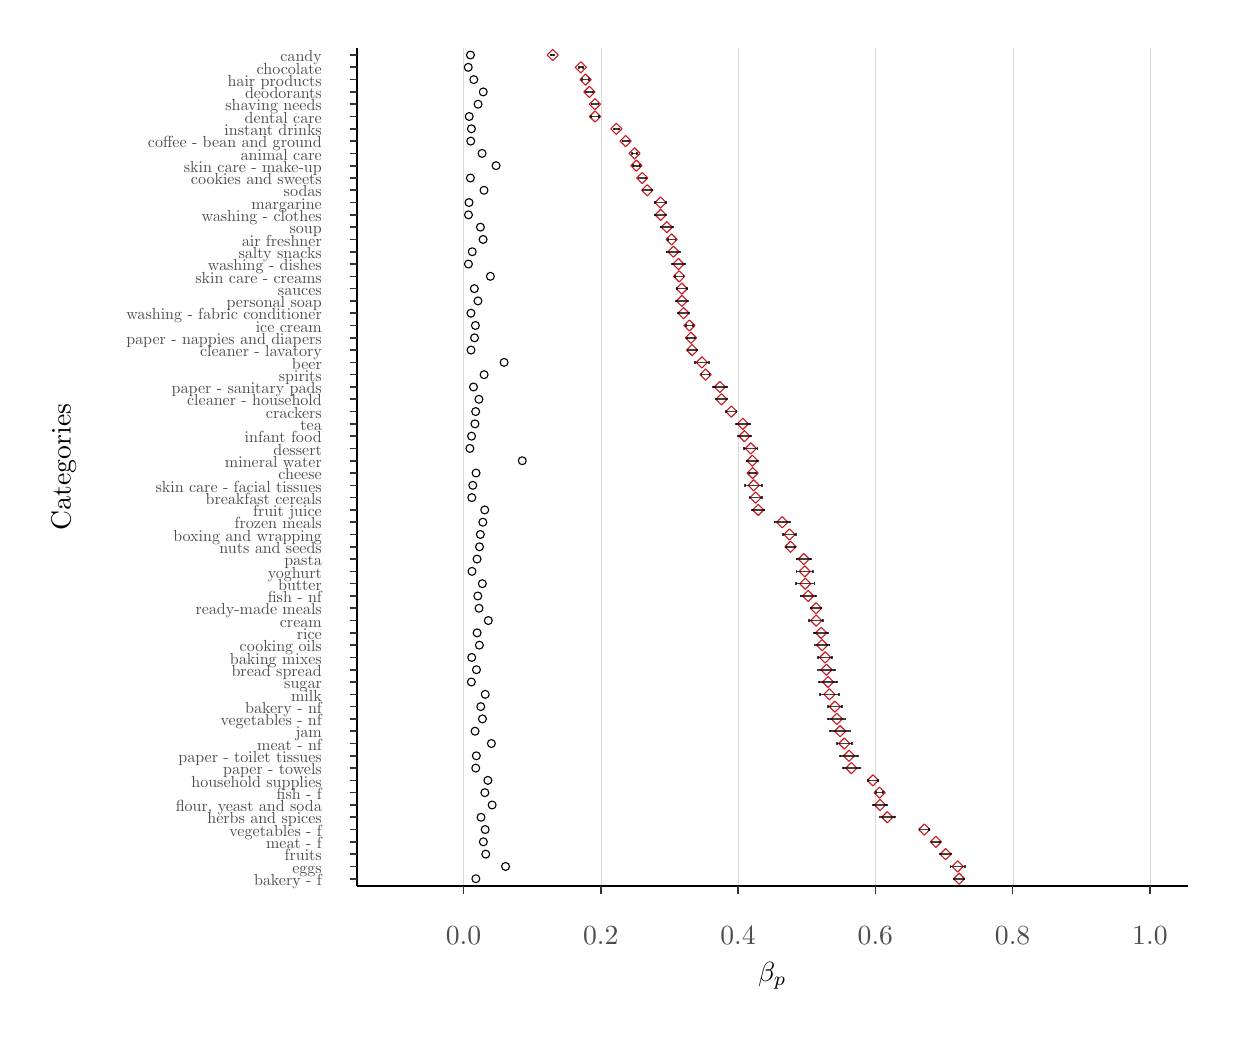
\begin{tikzpicture}[x=1pt,y=1pt]
\definecolor{fillColor}{RGB}{255,255,255}
\path[use as bounding box,fill=fillColor,fill opacity=0.00] (0,0) rectangle (433.62,361.35);
\begin{scope}
\path[clip] (  0.00,  0.00) rectangle (433.62,361.35);
\definecolor{drawColor}{RGB}{255,255,255}
\definecolor{fillColor}{RGB}{255,255,255}

\path[draw=drawColor,line width= 0.6pt,line join=round,line cap=round,fill=fillColor] (  0.00,  0.00) rectangle (433.62,361.35);
\end{scope}
\begin{scope}
\path[clip] (119.04, 51.15) rectangle (419.17,354.12);
\definecolor{drawColor}{RGB}{255,255,255}

\path[draw=drawColor,line width= 0.3pt,line join=round] (132.68, 51.15) --
	(132.68,354.12);

\path[draw=drawColor,line width= 0.3pt,line join=round] (182.29, 51.15) --
	(182.29,354.12);

\path[draw=drawColor,line width= 0.3pt,line join=round] (231.90, 51.15) --
	(231.90,354.12);

\path[draw=drawColor,line width= 0.3pt,line join=round] (281.51, 51.15) --
	(281.51,354.12);

\path[draw=drawColor,line width= 0.3pt,line join=round] (331.11, 51.15) --
	(331.11,354.12);

\path[draw=drawColor,line width= 0.3pt,line join=round] (380.72, 51.15) --
	(380.72,354.12);
\definecolor{drawColor}{gray}{0.85}

\path[draw=drawColor,line width= 0.1pt,line join=round] (157.49, 51.15) --
	(157.49,354.12);

\path[draw=drawColor,line width= 0.1pt,line join=round] (207.09, 51.15) --
	(207.09,354.12);

\path[draw=drawColor,line width= 0.1pt,line join=round] (256.70, 51.15) --
	(256.70,354.12);

\path[draw=drawColor,line width= 0.1pt,line join=round] (306.31, 51.15) --
	(306.31,354.12);

\path[draw=drawColor,line width= 0.1pt,line join=round] (355.92, 51.15) --
	(355.92,354.12);

\path[draw=drawColor,line width= 0.1pt,line join=round] (405.52, 51.15) --
	(405.52,354.12);
\definecolor{drawColor}{RGB}{0,0,0}

\path[draw=drawColor,line width= 0.4pt,line join=round,line cap=round] (164.56,284.82) circle (  1.43);

\path[draw=drawColor,line width= 0.4pt,line join=round,line cap=round] (164.19,315.92) circle (  1.43);

\path[draw=drawColor,line width= 0.4pt,line join=round,line cap=round] (161.95, 53.82) circle (  1.43);

\path[draw=drawColor,line width= 0.4pt,line join=round,line cap=round] (163.72,116.01) circle (  1.43);

\path[draw=drawColor,line width= 0.4pt,line join=round,line cap=round] (160.46,133.78) circle (  1.43);

\path[draw=drawColor,line width= 0.4pt,line join=round,line cap=round] (172.15,240.40) circle (  1.43);

\path[draw=drawColor,line width= 0.4pt,line join=round,line cap=round] (163.57,178.21) circle (  1.43);

\path[draw=drawColor,line width= 0.4pt,line join=round,line cap=round] (162.17,129.34) circle (  1.43);

\path[draw=drawColor,line width= 0.4pt,line join=round,line cap=round] (160.49,191.53) circle (  1.43);

\path[draw=drawColor,line width= 0.4pt,line join=round,line cap=round] (164.29,160.44) circle (  1.43);

\path[draw=drawColor,line width= 0.4pt,line join=round,line cap=round] (159.99,351.46) circle (  1.43);

\path[draw=drawColor,line width= 0.4pt,line join=round,line cap=round] (162.02,200.42) circle (  1.43);

\path[draw=drawColor,line width= 0.4pt,line join=round,line cap=round] (159.20,347.02) circle (  1.43);

\path[draw=drawColor,line width= 0.4pt,line join=round,line cap=round] (163.06,227.07) circle (  1.43);

\path[draw=drawColor,line width= 0.4pt,line join=round,line cap=round] (160.20,244.84) circle (  1.43);

\path[draw=drawColor,line width= 0.4pt,line join=round,line cap=round] (160.10,320.36) circle (  1.43);

\path[draw=drawColor,line width= 0.4pt,line join=round,line cap=round] (159.97,307.03) circle (  1.43);

\path[draw=drawColor,line width= 0.4pt,line join=round,line cap=round] (163.22,138.22) circle (  1.43);

\path[draw=drawColor,line width= 0.4pt,line join=round,line cap=round] (161.88,222.63) circle (  1.43);

\path[draw=drawColor,line width= 0.4pt,line join=round,line cap=round] (166.45,147.11) circle (  1.43);

\path[draw=drawColor,line width= 0.4pt,line join=round,line cap=round] (159.55,329.25) circle (  1.43);

\path[draw=drawColor,line width= 0.4pt,line join=round,line cap=round] (164.61,338.13) circle (  1.43);

\path[draw=drawColor,line width= 0.4pt,line join=round,line cap=round] (159.79,209.30) circle (  1.43);

\path[draw=drawColor,line width= 0.4pt,line join=round,line cap=round] (172.68, 58.26) circle (  1.43);

\path[draw=drawColor,line width= 0.4pt,line join=round,line cap=round] (165.20, 84.92) circle (  1.43);

\path[draw=drawColor,line width= 0.4pt,line join=round,line cap=round] (162.65,155.99) circle (  1.43);

\path[draw=drawColor,line width= 0.4pt,line join=round,line cap=round] (167.83, 80.47) circle (  1.43);

\path[draw=drawColor,line width= 0.4pt,line join=round,line cap=round] (164.47,182.65) circle (  1.43);

\path[draw=drawColor,line width= 0.4pt,line join=round,line cap=round] (165.16,187.09) circle (  1.43);

\path[draw=drawColor,line width= 0.4pt,line join=round,line cap=round] (165.53, 62.70) circle (  1.43);

\path[draw=drawColor,line width= 0.4pt,line join=round,line cap=round] (161.21,342.57) circle (  1.43);

\path[draw=drawColor,line width= 0.4pt,line join=round,line cap=round] (163.81, 76.03) circle (  1.43);

\path[draw=drawColor,line width= 0.4pt,line join=round,line cap=round] (166.29, 89.36) circle (  1.43);

\path[draw=drawColor,line width= 0.4pt,line join=round,line cap=round] (161.78,253.73) circle (  1.43);

\path[draw=drawColor,line width= 0.4pt,line join=round,line cap=round] (160.40,213.74) circle (  1.43);

\path[draw=drawColor,line width= 0.4pt,line join=round,line cap=round] (160.34,324.80) circle (  1.43);

\path[draw=drawColor,line width= 0.4pt,line join=round,line cap=round] (161.66,107.13) circle (  1.43);

\path[draw=drawColor,line width= 0.4pt,line join=round,line cap=round] (159.47,298.15) circle (  1.43);

\path[draw=drawColor,line width= 0.4pt,line join=round,line cap=round] (164.66, 67.15) circle (  1.43);

\path[draw=drawColor,line width= 0.4pt,line join=round,line cap=round] (167.56,102.69) circle (  1.43);

\path[draw=drawColor,line width= 0.4pt,line join=round,line cap=round] (165.34,120.45) circle (  1.43);

\path[draw=drawColor,line width= 0.4pt,line join=round,line cap=round] (178.72,204.86) circle (  1.43);

\path[draw=drawColor,line width= 0.4pt,line join=round,line cap=round] (163.26,173.76) circle (  1.43);

\path[draw=drawColor,line width= 0.4pt,line join=round,line cap=round] (161.47,249.28) circle (  1.43);

\path[draw=drawColor,line width= 0.4pt,line join=round,line cap=round] (161.09,231.51) circle (  1.43);

\path[draw=drawColor,line width= 0.4pt,line join=round,line cap=round] (162.12, 98.24) circle (  1.43);

\path[draw=drawColor,line width= 0.4pt,line join=round,line cap=round] (161.91, 93.80) circle (  1.43);

\path[draw=drawColor,line width= 0.4pt,line join=round,line cap=round] (162.38,169.32) circle (  1.43);

\path[draw=drawColor,line width= 0.4pt,line join=round,line cap=round] (162.71,262.61) circle (  1.43);

\path[draw=drawColor,line width= 0.4pt,line join=round,line cap=round] (163.09,151.55) circle (  1.43);

\path[draw=drawColor,line width= 0.4pt,line join=round,line cap=round] (162.40,142.67) circle (  1.43);

\path[draw=drawColor,line width= 0.4pt,line join=round,line cap=round] (160.64,280.38) circle (  1.43);

\path[draw=drawColor,line width= 0.4pt,line join=round,line cap=round] (161.41,267.05) circle (  1.43);

\path[draw=drawColor,line width= 0.4pt,line join=round,line cap=round] (162.75,333.69) circle (  1.43);

\path[draw=drawColor,line width= 0.4pt,line join=round,line cap=round] (167.20,271.49) circle (  1.43);

\path[draw=drawColor,line width= 0.4pt,line join=round,line cap=round] (160.84,195.97) circle (  1.43);

\path[draw=drawColor,line width= 0.4pt,line join=round,line cap=round] (169.26,311.48) circle (  1.43);

\path[draw=drawColor,line width= 0.4pt,line join=round,line cap=round] (164.89,302.59) circle (  1.43);

\path[draw=drawColor,line width= 0.4pt,line join=round,line cap=round] (163.59,289.26) circle (  1.43);

\path[draw=drawColor,line width= 0.4pt,line join=round,line cap=round] (164.93,235.96) circle (  1.43);

\path[draw=drawColor,line width= 0.4pt,line join=round,line cap=round] (160.33,124.90) circle (  1.43);

\path[draw=drawColor,line width= 0.4pt,line join=round,line cap=round] (161.62,218.19) circle (  1.43);

\path[draw=drawColor,line width= 0.4pt,line join=round,line cap=round] (165.32, 71.59) circle (  1.43);

\path[draw=drawColor,line width= 0.4pt,line join=round,line cap=round] (164.33,111.57) circle (  1.43);

\path[draw=drawColor,line width= 0.4pt,line join=round,line cap=round] (159.28,293.71) circle (  1.43);

\path[draw=drawColor,line width= 0.4pt,line join=round,line cap=round] (159.27,275.94) circle (  1.43);

\path[draw=drawColor,line width= 0.4pt,line join=round,line cap=round] (160.18,258.17) circle (  1.43);

\path[draw=drawColor,line width= 0.4pt,line join=round,line cap=round] (160.55,164.88) circle (  1.43);
\definecolor{drawColor}{RGB}{203,24,29}

\path[draw=drawColor,line width= 0.4pt,line join=round,line cap=round] (230.66,284.82) --
	(232.68,286.84) --
	(234.69,284.82) --
	(232.68,282.80) --
	cycle;

\path[draw=drawColor,line width= 0.4pt,line join=round,line cap=round] (217.27,315.92) --
	(219.28,317.94) --
	(221.30,315.92) --
	(219.28,313.90) --
	cycle;

\path[draw=drawColor,line width= 0.4pt,line join=round,line cap=round] (334.56, 53.82) --
	(336.57, 55.84) --
	(338.59, 53.82) --
	(336.57, 51.80) --
	cycle;

\path[draw=drawColor,line width= 0.4pt,line join=round,line cap=round] (289.70,116.01) --
	(291.71,118.03) --
	(293.73,116.01) --
	(291.71,113.99) --
	cycle;

\path[draw=drawColor,line width= 0.4pt,line join=round,line cap=round] (286.14,133.78) --
	(288.16,135.80) --
	(290.18,133.78) --
	(288.16,131.76) --
	cycle;

\path[draw=drawColor,line width= 0.4pt,line join=round,line cap=round] (241.62,240.40) --
	(243.64,242.42) --
	(245.66,240.40) --
	(243.64,238.38) --
	cycle;

\path[draw=drawColor,line width= 0.4pt,line join=round,line cap=round] (273.27,178.21) --
	(275.29,180.22) --
	(277.30,178.21) --
	(275.29,176.19) --
	cycle;

\path[draw=drawColor,line width= 0.4pt,line join=round,line cap=round] (286.60,129.34) --
	(288.62,131.36) --
	(290.64,129.34) --
	(288.62,127.32) --
	cycle;

\path[draw=drawColor,line width= 0.4pt,line join=round,line cap=round] (261.03,191.53) --
	(263.04,193.55) --
	(265.06,191.53) --
	(263.04,189.51) --
	cycle;

\path[draw=drawColor,line width= 0.4pt,line join=round,line cap=round] (278.96,160.44) --
	(280.98,162.45) --
	(283.00,160.44) --
	(280.98,158.42) --
	cycle;

\path[draw=drawColor,line width= 0.4pt,line join=round,line cap=round] (187.72,351.46) --
	(189.74,353.48) --
	(191.76,351.46) --
	(189.74,349.44) --
	cycle;

\path[draw=drawColor,line width= 0.4pt,line join=round,line cap=round] (259.94,200.42) --
	(261.96,202.43) --
	(263.98,200.42) --
	(261.96,198.40) --
	cycle;

\path[draw=drawColor,line width= 0.4pt,line join=round,line cap=round] (197.85,347.02) --
	(199.87,349.03) --
	(201.88,347.02) --
	(199.87,345.00) --
	cycle;

\path[draw=drawColor,line width= 0.4pt,line join=round,line cap=round] (248.69,227.07) --
	(250.70,229.09) --
	(252.72,227.07) --
	(250.70,225.05) --
	cycle;

\path[draw=drawColor,line width= 0.4pt,line join=round,line cap=round] (238.10,244.84) --
	(240.12,246.86) --
	(242.14,244.84) --
	(240.12,242.82) --
	cycle;

\path[draw=drawColor,line width= 0.4pt,line join=round,line cap=round] (214.07,320.36) --
	(216.09,322.38) --
	(218.11,320.36) --
	(216.09,318.34) --
	cycle;

\path[draw=drawColor,line width= 0.4pt,line join=round,line cap=round] (220.04,307.03) --
	(222.06,309.05) --
	(224.08,307.03) --
	(222.06,305.02) --
	cycle;

\path[draw=drawColor,line width= 0.4pt,line join=round,line cap=round] (285.04,138.22) --
	(287.06,140.24) --
	(289.07,138.22) --
	(287.06,136.21) --
	cycle;

\path[draw=drawColor,line width= 0.4pt,line join=round,line cap=round] (252.26,222.63) --
	(254.27,224.65) --
	(256.29,222.63) --
	(254.27,220.61) --
	cycle;

\path[draw=drawColor,line width= 0.4pt,line join=round,line cap=round] (282.90,147.11) --
	(284.92,149.13) --
	(286.93,147.11) --
	(284.92,145.09) --
	cycle;

\path[draw=drawColor,line width= 0.4pt,line join=round,line cap=round] (203.00,329.25) --
	(205.02,331.26) --
	(207.04,329.25) --
	(205.02,327.23) --
	cycle;

\path[draw=drawColor,line width= 0.4pt,line join=round,line cap=round] (200.97,338.13) --
	(202.99,340.15) --
	(205.00,338.13) --
	(202.99,336.11) --
	cycle;

\path[draw=drawColor,line width= 0.4pt,line join=round,line cap=round] (259.31,209.30) --
	(261.33,211.32) --
	(263.35,209.30) --
	(261.33,207.28) --
	cycle;

\path[draw=drawColor,line width= 0.4pt,line join=round,line cap=round] (334.05, 58.26) --
	(336.06, 60.28) --
	(338.08, 58.26) --
	(336.06, 56.24) --
	cycle;

\path[draw=drawColor,line width= 0.4pt,line join=round,line cap=round] (305.81, 84.92) --
	(307.82, 86.93) --
	(309.84, 84.92) --
	(307.82, 82.90) --
	cycle;

\path[draw=drawColor,line width= 0.4pt,line join=round,line cap=round] (280.01,155.99) --
	(282.03,158.01) --
	(284.04,155.99) --
	(282.03,153.98) --
	cycle;

\path[draw=drawColor,line width= 0.4pt,line join=round,line cap=round] (305.98, 80.47) --
	(307.99, 82.49) --
	(310.01, 80.47) --
	(307.99, 78.46) --
	cycle;

\path[draw=drawColor,line width= 0.4pt,line join=round,line cap=round] (270.64,182.65) --
	(272.66,184.67) --
	(274.68,182.65) --
	(272.66,180.63) --
	cycle;

\path[draw=drawColor,line width= 0.4pt,line join=round,line cap=round] (261.98,187.09) --
	(264.00,189.11) --
	(266.02,187.09) --
	(264.00,185.07) --
	cycle;

\path[draw=drawColor,line width= 0.4pt,line join=round,line cap=round] (329.70, 62.70) --
	(331.72, 64.72) --
	(333.74, 62.70) --
	(331.72, 60.69) --
	cycle;

\path[draw=drawColor,line width= 0.4pt,line join=round,line cap=round] (199.57,342.57) --
	(201.59,344.59) --
	(203.61,342.57) --
	(201.59,340.56) --
	cycle;

\path[draw=drawColor,line width= 0.4pt,line join=round,line cap=round] (308.61, 76.03) --
	(310.63, 78.05) --
	(312.64, 76.03) --
	(310.63, 74.01) --
	cycle;

\path[draw=drawColor,line width= 0.4pt,line join=round,line cap=round] (303.43, 89.36) --
	(305.45, 91.38) --
	(307.47, 89.36) --
	(305.45, 87.34) --
	cycle;

\path[draw=drawColor,line width= 0.4pt,line join=round,line cap=round] (237.11,253.73) --
	(239.12,255.74) --
	(241.14,253.73) --
	(239.12,251.71) --
	cycle;

\path[draw=drawColor,line width= 0.4pt,line join=round,line cap=round] (256.99,213.74) --
	(259.00,215.76) --
	(261.02,213.74) --
	(259.00,211.73) --
	cycle;

\path[draw=drawColor,line width= 0.4pt,line join=round,line cap=round] (210.69,324.80) --
	(212.71,326.82) --
	(214.73,324.80) --
	(212.71,322.79) --
	cycle;

\path[draw=drawColor,line width= 0.4pt,line join=round,line cap=round] (291.56,107.13) --
	(293.58,109.14) --
	(295.60,107.13) --
	(293.58,105.11) --
	cycle;

\path[draw=drawColor,line width= 0.4pt,line join=round,line cap=round] (226.67,298.15) --
	(228.69,300.17) --
	(230.71,298.15) --
	(228.69,296.13) --
	cycle;

\path[draw=drawColor,line width= 0.4pt,line join=round,line cap=round] (326.13, 67.15) --
	(328.15, 69.16) --
	(330.17, 67.15) --
	(328.15, 65.13) --
	cycle;

\path[draw=drawColor,line width= 0.4pt,line join=round,line cap=round] (293.07,102.69) --
	(295.09,104.70) --
	(297.11,102.69) --
	(295.09,100.67) --
	cycle;

\path[draw=drawColor,line width= 0.4pt,line join=round,line cap=round] (287.70,120.45) --
	(289.72,122.47) --
	(291.74,120.45) --
	(289.72,118.44) --
	cycle;

\path[draw=drawColor,line width= 0.4pt,line join=round,line cap=round] (259.85,204.86) --
	(261.86,206.88) --
	(263.88,204.86) --
	(261.86,202.84) --
	cycle;

\path[draw=drawColor,line width= 0.4pt,line join=round,line cap=round] (273.64,173.76) --
	(275.66,175.78) --
	(277.68,173.76) --
	(275.66,171.75) --
	cycle;

\path[draw=drawColor,line width= 0.4pt,line join=round,line cap=round] (237.66,249.28) --
	(239.68,251.30) --
	(241.70,249.28) --
	(239.68,247.27) --
	cycle;

\path[draw=drawColor,line width= 0.4pt,line join=round,line cap=round] (248.10,231.51) --
	(250.12,233.53) --
	(252.13,231.51) --
	(250.12,229.50) --
	cycle;

\path[draw=drawColor,line width= 0.4pt,line join=round,line cap=round] (294.77, 98.24) --
	(296.79,100.26) --
	(298.80, 98.24) --
	(296.79, 96.23) --
	cycle;

\path[draw=drawColor,line width= 0.4pt,line join=round,line cap=round] (295.64, 93.80) --
	(297.65, 95.82) --
	(299.67, 93.80) --
	(297.65, 91.78) --
	cycle;

\path[draw=drawColor,line width= 0.4pt,line join=round,line cap=round] (278.40,169.32) --
	(280.42,171.34) --
	(282.44,169.32) --
	(280.42,167.30) --
	cycle;

\path[draw=drawColor,line width= 0.4pt,line join=round,line cap=round] (234.39,262.61) --
	(236.41,264.63) --
	(238.42,262.61) --
	(236.41,260.59) --
	cycle;

\path[draw=drawColor,line width= 0.4pt,line join=round,line cap=round] (282.86,151.55) --
	(284.88,153.57) --
	(286.90,151.55) --
	(284.88,149.53) --
	cycle;

\path[draw=drawColor,line width= 0.4pt,line join=round,line cap=round] (284.71,142.67) --
	(286.73,144.68) --
	(288.75,142.67) --
	(286.73,140.65) --
	cycle;

\path[draw=drawColor,line width= 0.4pt,line join=round,line cap=round] (231.31,280.38) --
	(233.33,282.40) --
	(235.34,280.38) --
	(233.33,278.36) --
	cycle;

\path[draw=drawColor,line width= 0.4pt,line join=round,line cap=round] (234.34,267.05) --
	(236.36,269.07) --
	(238.38,267.05) --
	(236.36,265.04) --
	cycle;

\path[draw=drawColor,line width= 0.4pt,line join=round,line cap=round] (202.96,333.69) --
	(204.98,335.71) --
	(206.99,333.69) --
	(204.98,331.67) --
	cycle;

\path[draw=drawColor,line width= 0.4pt,line join=round,line cap=round] (233.41,271.49) --
	(235.42,273.51) --
	(237.44,271.49) --
	(235.42,269.48) --
	cycle;

\path[draw=drawColor,line width= 0.4pt,line join=round,line cap=round] (260.34,195.97) --
	(262.36,197.99) --
	(264.37,195.97) --
	(262.36,193.96) --
	cycle;

\path[draw=drawColor,line width= 0.4pt,line join=round,line cap=round] (217.93,311.48) --
	(219.95,313.49) --
	(221.97,311.48) --
	(219.95,309.46) --
	cycle;

\path[draw=drawColor,line width= 0.4pt,line join=round,line cap=round] (221.87,302.59) --
	(223.88,304.61) --
	(225.90,302.59) --
	(223.88,300.57) --
	cycle;

\path[draw=drawColor,line width= 0.4pt,line join=round,line cap=round] (228.92,289.26) --
	(230.94,291.28) --
	(232.96,289.26) --
	(230.94,287.25) --
	cycle;

\path[draw=drawColor,line width= 0.4pt,line join=round,line cap=round] (242.94,235.96) --
	(244.96,237.97) --
	(246.98,235.96) --
	(244.96,233.94) --
	cycle;

\path[draw=drawColor,line width= 0.4pt,line join=round,line cap=round] (287.21,124.90) --
	(289.23,126.91) --
	(291.25,124.90) --
	(289.23,122.88) --
	cycle;

\path[draw=drawColor,line width= 0.4pt,line join=round,line cap=round] (256.40,218.19) --
	(258.42,220.20) --
	(260.44,218.19) --
	(258.42,216.17) --
	cycle;

\path[draw=drawColor,line width= 0.4pt,line join=round,line cap=round] (321.96, 71.59) --
	(323.98, 73.61) --
	(326.00, 71.59) --
	(323.98, 69.57) --
	cycle;

\path[draw=drawColor,line width= 0.4pt,line join=round,line cap=round] (290.39,111.57) --
	(292.40,113.59) --
	(294.42,111.57) --
	(292.40,109.55) --
	cycle;

\path[draw=drawColor,line width= 0.4pt,line join=round,line cap=round] (226.72,293.71) --
	(228.74,295.72) --
	(230.76,293.71) --
	(228.74,291.69) --
	cycle;

\path[draw=drawColor,line width= 0.4pt,line join=round,line cap=round] (233.14,275.94) --
	(235.16,277.95) --
	(237.17,275.94) --
	(235.16,273.92) --
	cycle;

\path[draw=drawColor,line width= 0.4pt,line join=round,line cap=round] (234.99,258.17) --
	(237.01,260.19) --
	(239.03,258.17) --
	(237.01,256.15) --
	cycle;

\path[draw=drawColor,line width= 0.4pt,line join=round,line cap=round] (278.78,164.88) --
	(280.80,166.90) --
	(282.81,164.88) --
	(280.80,162.86) --
	cycle;
\definecolor{drawColor}{RGB}{0,0,0}

\path[draw=drawColor,draw opacity=0.75,line width= 0.6pt,line join=round] (234.07,284.38) --
	(234.07,285.27);

\path[draw=drawColor,draw opacity=0.75,line width= 0.6pt,line join=round] (234.07,284.82) --
	(231.29,284.82);

\path[draw=drawColor,draw opacity=0.75,line width= 0.6pt,line join=round] (231.29,284.38) --
	(231.29,285.27);

\path[draw=drawColor,draw opacity=0.75,line width= 0.6pt,line join=round] (220.14,315.47) --
	(220.14,316.36);

\path[draw=drawColor,draw opacity=0.75,line width= 0.6pt,line join=round] (220.14,315.92) --
	(218.42,315.92);

\path[draw=drawColor,draw opacity=0.75,line width= 0.6pt,line join=round] (218.42,315.47) --
	(218.42,316.36);

\path[draw=drawColor,draw opacity=0.75,line width= 0.6pt,line join=round] (338.35, 53.37) --
	(338.35, 54.26);

\path[draw=drawColor,draw opacity=0.75,line width= 0.6pt,line join=round] (338.35, 53.82) --
	(334.80, 53.82);

\path[draw=drawColor,draw opacity=0.75,line width= 0.6pt,line join=round] (334.80, 53.37) --
	(334.80, 54.26);

\path[draw=drawColor,draw opacity=0.75,line width= 0.6pt,line join=round] (294.18,115.57) --
	(294.18,116.46);

\path[draw=drawColor,draw opacity=0.75,line width= 0.6pt,line join=round] (294.18,116.01) --
	(289.25,116.01);

\path[draw=drawColor,draw opacity=0.75,line width= 0.6pt,line join=round] (289.25,115.57) --
	(289.25,116.46);

\path[draw=drawColor,draw opacity=0.75,line width= 0.6pt,line join=round] (290.69,133.34) --
	(290.69,134.23);

\path[draw=drawColor,draw opacity=0.75,line width= 0.6pt,line join=round] (290.69,133.78) --
	(285.63,133.78);

\path[draw=drawColor,draw opacity=0.75,line width= 0.6pt,line join=round] (285.63,133.34) --
	(285.63,134.23);

\path[draw=drawColor,draw opacity=0.75,line width= 0.6pt,line join=round] (246.21,239.95) --
	(246.21,240.84);

\path[draw=drawColor,draw opacity=0.75,line width= 0.6pt,line join=round] (246.21,240.40) --
	(241.07,240.40);

\path[draw=drawColor,draw opacity=0.75,line width= 0.6pt,line join=round] (241.07,239.95) --
	(241.07,240.84);

\path[draw=drawColor,draw opacity=0.75,line width= 0.6pt,line join=round] (277.69,177.76) --
	(277.69,178.65);

\path[draw=drawColor,draw opacity=0.75,line width= 0.6pt,line join=round] (277.69,178.21) --
	(272.88,178.21);

\path[draw=drawColor,draw opacity=0.75,line width= 0.6pt,line join=round] (272.88,177.76) --
	(272.88,178.65);

\path[draw=drawColor,draw opacity=0.75,line width= 0.6pt,line join=round] (291.83,128.90) --
	(291.83,129.78);

\path[draw=drawColor,draw opacity=0.75,line width= 0.6pt,line join=round] (291.83,129.34) --
	(285.41,129.34);

\path[draw=drawColor,draw opacity=0.75,line width= 0.6pt,line join=round] (285.41,128.90) --
	(285.41,129.78);

\path[draw=drawColor,draw opacity=0.75,line width= 0.6pt,line join=round] (265.30,191.09) --
	(265.30,191.98);

\path[draw=drawColor,draw opacity=0.75,line width= 0.6pt,line join=round] (265.30,191.53) --
	(260.79,191.53);

\path[draw=drawColor,draw opacity=0.75,line width= 0.6pt,line join=round] (260.79,191.09) --
	(260.79,191.98);

\path[draw=drawColor,draw opacity=0.75,line width= 0.6pt,line join=round] (284.26,159.99) --
	(284.26,160.88);

\path[draw=drawColor,draw opacity=0.75,line width= 0.6pt,line join=round] (284.26,160.44) --
	(277.70,160.44);

\path[draw=drawColor,draw opacity=0.75,line width= 0.6pt,line join=round] (277.70,159.99) --
	(277.70,160.88);

\path[draw=drawColor,draw opacity=0.75,line width= 0.6pt,line join=round] (190.27,351.01) --
	(190.27,351.90);

\path[draw=drawColor,draw opacity=0.75,line width= 0.6pt,line join=round] (190.27,351.46) --
	(189.22,351.46);

\path[draw=drawColor,draw opacity=0.75,line width= 0.6pt,line join=round] (189.22,351.01) --
	(189.22,351.90);

\path[draw=drawColor,draw opacity=0.75,line width= 0.6pt,line join=round] (263.17,199.97) --
	(263.17,200.86);

\path[draw=drawColor,draw opacity=0.75,line width= 0.6pt,line join=round] (263.17,200.42) --
	(260.75,200.42);

\path[draw=drawColor,draw opacity=0.75,line width= 0.6pt,line join=round] (260.75,199.97) --
	(260.75,200.86);

\path[draw=drawColor,draw opacity=0.75,line width= 0.6pt,line join=round] (200.55,346.57) --
	(200.55,347.46);

\path[draw=drawColor,draw opacity=0.75,line width= 0.6pt,line join=round] (200.55,347.02) --
	(199.18,347.02);

\path[draw=drawColor,draw opacity=0.75,line width= 0.6pt,line join=round] (199.18,346.57) --
	(199.18,347.46);

\path[draw=drawColor,draw opacity=0.75,line width= 0.6pt,line join=round] (252.67,226.63) --
	(252.67,227.52);

\path[draw=drawColor,draw opacity=0.75,line width= 0.6pt,line join=round] (252.67,227.07) --
	(248.74,227.07);

\path[draw=drawColor,draw opacity=0.75,line width= 0.6pt,line join=round] (248.74,226.63) --
	(248.74,227.52);

\path[draw=drawColor,draw opacity=0.75,line width= 0.6pt,line join=round] (241.86,244.40) --
	(241.86,245.29);

\path[draw=drawColor,draw opacity=0.75,line width= 0.6pt,line join=round] (241.86,244.84) --
	(238.38,244.84);

\path[draw=drawColor,draw opacity=0.75,line width= 0.6pt,line join=round] (238.38,244.40) --
	(238.38,245.29);

\path[draw=drawColor,draw opacity=0.75,line width= 0.6pt,line join=round] (217.30,319.92) --
	(217.30,320.81);

\path[draw=drawColor,draw opacity=0.75,line width= 0.6pt,line join=round] (217.30,320.36) --
	(214.88,320.36);

\path[draw=drawColor,draw opacity=0.75,line width= 0.6pt,line join=round] (214.88,319.92) --
	(214.88,320.81);

\path[draw=drawColor,draw opacity=0.75,line width= 0.6pt,line join=round] (223.38,306.59) --
	(223.38,307.48);

\path[draw=drawColor,draw opacity=0.75,line width= 0.6pt,line join=round] (223.38,307.03) --
	(220.74,307.03);

\path[draw=drawColor,draw opacity=0.75,line width= 0.6pt,line join=round] (220.74,306.59) --
	(220.74,307.48);

\path[draw=drawColor,draw opacity=0.75,line width= 0.6pt,line join=round] (289.76,137.78) --
	(289.76,138.67);

\path[draw=drawColor,draw opacity=0.75,line width= 0.6pt,line join=round] (289.76,138.22) --
	(284.35,138.22);

\path[draw=drawColor,draw opacity=0.75,line width= 0.6pt,line join=round] (284.35,137.78) --
	(284.35,138.67);

\path[draw=drawColor,draw opacity=0.75,line width= 0.6pt,line join=round] (256.10,222.18) --
	(256.10,223.07);

\path[draw=drawColor,draw opacity=0.75,line width= 0.6pt,line join=round] (256.10,222.63) --
	(252.45,222.63);

\path[draw=drawColor,draw opacity=0.75,line width= 0.6pt,line join=round] (252.45,222.18) --
	(252.45,223.07);

\path[draw=drawColor,draw opacity=0.75,line width= 0.6pt,line join=round] (287.43,146.66) --
	(287.43,147.55);

\path[draw=drawColor,draw opacity=0.75,line width= 0.6pt,line join=round] (287.43,147.11) --
	(282.41,147.11);

\path[draw=drawColor,draw opacity=0.75,line width= 0.6pt,line join=round] (282.41,146.66) --
	(282.41,147.55);

\path[draw=drawColor,draw opacity=0.75,line width= 0.6pt,line join=round] (206.40,328.80) --
	(206.40,329.69);

\path[draw=drawColor,draw opacity=0.75,line width= 0.6pt,line join=round] (206.40,329.25) --
	(203.63,329.25);

\path[draw=drawColor,draw opacity=0.75,line width= 0.6pt,line join=round] (203.63,328.80) --
	(203.63,329.69);

\path[draw=drawColor,draw opacity=0.75,line width= 0.6pt,line join=round] (204.24,337.69) --
	(204.24,338.57);

\path[draw=drawColor,draw opacity=0.75,line width= 0.6pt,line join=round] (204.24,338.13) --
	(201.73,338.13);

\path[draw=drawColor,draw opacity=0.75,line width= 0.6pt,line join=round] (201.73,337.69) --
	(201.73,338.57);

\path[draw=drawColor,draw opacity=0.75,line width= 0.6pt,line join=round] (263.74,208.86) --
	(263.74,209.75);

\path[draw=drawColor,draw opacity=0.75,line width= 0.6pt,line join=round] (263.74,209.30) --
	(258.92,209.30);

\path[draw=drawColor,draw opacity=0.75,line width= 0.6pt,line join=round] (258.92,208.86) --
	(258.92,209.75);

\path[draw=drawColor,draw opacity=0.75,line width= 0.6pt,line join=round] (338.68, 57.82) --
	(338.68, 58.71);

\path[draw=drawColor,draw opacity=0.75,line width= 0.6pt,line join=round] (338.68, 58.26) --
	(333.45, 58.26);

\path[draw=drawColor,draw opacity=0.75,line width= 0.6pt,line join=round] (333.45, 57.82) --
	(333.45, 58.71);

\path[draw=drawColor,draw opacity=0.75,line width= 0.6pt,line join=round] (309.04, 84.47) --
	(309.04, 85.36);

\path[draw=drawColor,draw opacity=0.75,line width= 0.6pt,line join=round] (309.04, 84.92) --
	(306.61, 84.92);

\path[draw=drawColor,draw opacity=0.75,line width= 0.6pt,line join=round] (306.61, 84.47) --
	(306.61, 85.36);

\path[draw=drawColor,draw opacity=0.75,line width= 0.6pt,line join=round] (284.82,155.55) --
	(284.82,156.44);

\path[draw=drawColor,draw opacity=0.75,line width= 0.6pt,line join=round] (284.82,155.99) --
	(279.24,155.99);

\path[draw=drawColor,draw opacity=0.75,line width= 0.6pt,line join=round] (279.24,155.55) --
	(279.24,156.44);

\path[draw=drawColor,draw opacity=0.75,line width= 0.6pt,line join=round] (310.57, 80.03) --
	(310.57, 80.92);

\path[draw=drawColor,draw opacity=0.75,line width= 0.6pt,line join=round] (310.57, 80.47) --
	(305.42, 80.47);

\path[draw=drawColor,draw opacity=0.75,line width= 0.6pt,line join=round] (305.42, 80.03) --
	(305.42, 80.92);

\path[draw=drawColor,draw opacity=0.75,line width= 0.6pt,line join=round] (275.50,182.20) --
	(275.50,183.09);

\path[draw=drawColor,draw opacity=0.75,line width= 0.6pt,line join=round] (275.50,182.65) --
	(269.81,182.65);

\path[draw=drawColor,draw opacity=0.75,line width= 0.6pt,line join=round] (269.81,182.20) --
	(269.81,183.09);

\path[draw=drawColor,draw opacity=0.75,line width= 0.6pt,line join=round] (266.29,186.65) --
	(266.29,187.53);

\path[draw=drawColor,draw opacity=0.75,line width= 0.6pt,line join=round] (266.29,187.09) --
	(261.71,187.09);

\path[draw=drawColor,draw opacity=0.75,line width= 0.6pt,line join=round] (261.71,186.65) --
	(261.71,187.53);

\path[draw=drawColor,draw opacity=0.75,line width= 0.6pt,line join=round] (333.79, 62.26) --
	(333.79, 63.15);

\path[draw=drawColor,draw opacity=0.75,line width= 0.6pt,line join=round] (333.79, 62.70) --
	(329.65, 62.70);

\path[draw=drawColor,draw opacity=0.75,line width= 0.6pt,line join=round] (329.65, 62.26) --
	(329.65, 63.15);

\path[draw=drawColor,draw opacity=0.75,line width= 0.6pt,line join=round] (202.95,342.13) --
	(202.95,343.02);

\path[draw=drawColor,draw opacity=0.75,line width= 0.6pt,line join=round] (202.95,342.57) --
	(200.24,342.57);

\path[draw=drawColor,draw opacity=0.75,line width= 0.6pt,line join=round] (200.24,342.13) --
	(200.24,343.02);

\path[draw=drawColor,draw opacity=0.75,line width= 0.6pt,line join=round] (313.40, 75.59) --
	(313.40, 76.48);

\path[draw=drawColor,draw opacity=0.75,line width= 0.6pt,line join=round] (313.40, 76.03) --
	(307.85, 76.03);

\path[draw=drawColor,draw opacity=0.75,line width= 0.6pt,line join=round] (307.85, 75.59) --
	(307.85, 76.48);

\path[draw=drawColor,draw opacity=0.75,line width= 0.6pt,line join=round] (307.28, 88.91) --
	(307.28, 89.80);

\path[draw=drawColor,draw opacity=0.75,line width= 0.6pt,line join=round] (307.28, 89.36) --
	(303.62, 89.36);

\path[draw=drawColor,draw opacity=0.75,line width= 0.6pt,line join=round] (303.62, 88.91) --
	(303.62, 89.80);

\path[draw=drawColor,draw opacity=0.75,line width= 0.6pt,line join=round] (240.46,253.28) --
	(240.46,254.17);

\path[draw=drawColor,draw opacity=0.75,line width= 0.6pt,line join=round] (240.46,253.73) --
	(237.79,253.73);

\path[draw=drawColor,draw opacity=0.75,line width= 0.6pt,line join=round] (237.79,253.28) --
	(237.79,254.17);

\path[draw=drawColor,draw opacity=0.75,line width= 0.6pt,line join=round] (261.39,213.30) --
	(261.39,214.19);

\path[draw=drawColor,draw opacity=0.75,line width= 0.6pt,line join=round] (261.39,213.74) --
	(256.61,213.74);

\path[draw=drawColor,draw opacity=0.75,line width= 0.6pt,line join=round] (256.61,213.30) --
	(256.61,214.19);

\path[draw=drawColor,draw opacity=0.75,line width= 0.6pt,line join=round] (213.56,324.36) --
	(213.56,325.25);

\path[draw=drawColor,draw opacity=0.75,line width= 0.6pt,line join=round] (213.56,324.80) --
	(211.86,324.80);

\path[draw=drawColor,draw opacity=0.75,line width= 0.6pt,line join=round] (211.86,324.36) --
	(211.86,325.25);

\path[draw=drawColor,draw opacity=0.75,line width= 0.6pt,line join=round] (297.28,106.68) --
	(297.28,107.57);

\path[draw=drawColor,draw opacity=0.75,line width= 0.6pt,line join=round] (297.28,107.13) --
	(289.88,107.13);

\path[draw=drawColor,draw opacity=0.75,line width= 0.6pt,line join=round] (289.88,106.68) --
	(289.88,107.57);

\path[draw=drawColor,draw opacity=0.75,line width= 0.6pt,line join=round] (230.73,297.70) --
	(230.73,298.59);

\path[draw=drawColor,draw opacity=0.75,line width= 0.6pt,line join=round] (230.73,298.15) --
	(226.65,298.15);

\path[draw=drawColor,draw opacity=0.75,line width= 0.6pt,line join=round] (226.65,297.70) --
	(226.65,298.59);

\path[draw=drawColor,draw opacity=0.75,line width= 0.6pt,line join=round] (329.73, 66.70) --
	(329.73, 67.59);

\path[draw=drawColor,draw opacity=0.75,line width= 0.6pt,line join=round] (329.73, 67.15) --
	(326.57, 67.15);

\path[draw=drawColor,draw opacity=0.75,line width= 0.6pt,line join=round] (326.57, 66.70) --
	(326.57, 67.59);

\path[draw=drawColor,draw opacity=0.75,line width= 0.6pt,line join=round] (297.85,102.24) --
	(297.85,103.13);

\path[draw=drawColor,draw opacity=0.75,line width= 0.6pt,line join=round] (297.85,102.69) --
	(292.33,102.69);

\path[draw=drawColor,draw opacity=0.75,line width= 0.6pt,line join=round] (292.33,102.24) --
	(292.33,103.13);

\path[draw=drawColor,draw opacity=0.75,line width= 0.6pt,line join=round] (293.23,120.01) --
	(293.23,120.90);

\path[draw=drawColor,draw opacity=0.75,line width= 0.6pt,line join=round] (293.23,120.45) --
	(286.21,120.45);

\path[draw=drawColor,draw opacity=0.75,line width= 0.6pt,line join=round] (286.21,120.01) --
	(286.21,120.90);

\path[draw=drawColor,draw opacity=0.75,line width= 0.6pt,line join=round] (264.01,204.42) --
	(264.01,205.30);

\path[draw=drawColor,draw opacity=0.75,line width= 0.6pt,line join=round] (264.01,204.86) --
	(259.72,204.86);

\path[draw=drawColor,draw opacity=0.75,line width= 0.6pt,line join=round] (259.72,204.42) --
	(259.72,205.30);

\path[draw=drawColor,draw opacity=0.75,line width= 0.6pt,line join=round] (277.37,173.32) --
	(277.37,174.21);

\path[draw=drawColor,draw opacity=0.75,line width= 0.6pt,line join=round] (277.37,173.76) --
	(273.95,173.76);

\path[draw=drawColor,draw opacity=0.75,line width= 0.6pt,line join=round] (273.95,173.32) --
	(273.95,174.21);

\path[draw=drawColor,draw opacity=0.75,line width= 0.6pt,line join=round] (241.13,248.84) --
	(241.13,249.73);

\path[draw=drawColor,draw opacity=0.75,line width= 0.6pt,line join=round] (241.13,249.28) --
	(238.23,249.28);

\path[draw=drawColor,draw opacity=0.75,line width= 0.6pt,line join=round] (238.23,248.84) --
	(238.23,249.73);

\path[draw=drawColor,draw opacity=0.75,line width= 0.6pt,line join=round] (252.70,231.07) --
	(252.70,231.96);

\path[draw=drawColor,draw opacity=0.75,line width= 0.6pt,line join=round] (252.70,231.51) --
	(247.53,231.51);

\path[draw=drawColor,draw opacity=0.75,line width= 0.6pt,line join=round] (247.53,231.07) --
	(247.53,231.96);

\path[draw=drawColor,draw opacity=0.75,line width= 0.6pt,line join=round] (300.12, 97.80) --
	(300.12, 98.69);

\path[draw=drawColor,draw opacity=0.75,line width= 0.6pt,line join=round] (300.12, 98.24) --
	(293.46, 98.24);

\path[draw=drawColor,draw opacity=0.75,line width= 0.6pt,line join=round] (293.46, 97.80) --
	(293.46, 98.69);

\path[draw=drawColor,draw opacity=0.75,line width= 0.6pt,line join=round] (300.80, 93.36) --
	(300.80, 94.24);

\path[draw=drawColor,draw opacity=0.75,line width= 0.6pt,line join=round] (300.80, 93.80) --
	(294.51, 93.80);

\path[draw=drawColor,draw opacity=0.75,line width= 0.6pt,line join=round] (294.51, 93.36) --
	(294.51, 94.24);

\path[draw=drawColor,draw opacity=0.75,line width= 0.6pt,line join=round] (283.09,168.88) --
	(283.09,169.76);

\path[draw=drawColor,draw opacity=0.75,line width= 0.6pt,line join=round] (283.09,169.32) --
	(277.75,169.32);

\path[draw=drawColor,draw opacity=0.75,line width= 0.6pt,line join=round] (277.75,168.88) --
	(277.75,169.76);

\path[draw=drawColor,draw opacity=0.75,line width= 0.6pt,line join=round] (238.58,262.17) --
	(238.58,263.05);

\path[draw=drawColor,draw opacity=0.75,line width= 0.6pt,line join=round] (238.58,262.61) --
	(234.23,262.61);

\path[draw=drawColor,draw opacity=0.75,line width= 0.6pt,line join=round] (234.23,262.17) --
	(234.23,263.05);

\path[draw=drawColor,draw opacity=0.75,line width= 0.6pt,line join=round] (286.89,151.11) --
	(286.89,152.00);

\path[draw=drawColor,draw opacity=0.75,line width= 0.6pt,line join=round] (286.89,151.55) --
	(282.87,151.55);

\path[draw=drawColor,draw opacity=0.75,line width= 0.6pt,line join=round] (282.87,151.11) --
	(282.87,152.00);

\path[draw=drawColor,draw opacity=0.75,line width= 0.6pt,line join=round] (289.23,142.22) --
	(289.23,143.11);

\path[draw=drawColor,draw opacity=0.75,line width= 0.6pt,line join=round] (289.23,142.67) --
	(284.22,142.67);

\path[draw=drawColor,draw opacity=0.75,line width= 0.6pt,line join=round] (284.22,142.22) --
	(284.22,143.11);

\path[draw=drawColor,draw opacity=0.75,line width= 0.6pt,line join=round] (235.84,279.94) --
	(235.84,280.82);

\path[draw=drawColor,draw opacity=0.75,line width= 0.6pt,line join=round] (235.84,280.38) --
	(230.82,280.38);

\path[draw=drawColor,draw opacity=0.75,line width= 0.6pt,line join=round] (230.82,279.94) --
	(230.82,280.82);

\path[draw=drawColor,draw opacity=0.75,line width= 0.6pt,line join=round] (238.18,266.61) --
	(238.18,267.50);

\path[draw=drawColor,draw opacity=0.75,line width= 0.6pt,line join=round] (238.18,267.05) --
	(234.54,267.05);

\path[draw=drawColor,draw opacity=0.75,line width= 0.6pt,line join=round] (234.54,266.61) --
	(234.54,267.50);

\path[draw=drawColor,draw opacity=0.75,line width= 0.6pt,line join=round] (206.27,333.24) --
	(206.27,334.13);

\path[draw=drawColor,draw opacity=0.75,line width= 0.6pt,line join=round] (206.27,333.69) --
	(203.68,333.69);

\path[draw=drawColor,draw opacity=0.75,line width= 0.6pt,line join=round] (203.68,333.24) --
	(203.68,334.13);

\path[draw=drawColor,draw opacity=0.75,line width= 0.6pt,line join=round] (236.98,271.05) --
	(236.98,271.94);

\path[draw=drawColor,draw opacity=0.75,line width= 0.6pt,line join=round] (236.98,271.49) --
	(233.87,271.49);

\path[draw=drawColor,draw opacity=0.75,line width= 0.6pt,line join=round] (233.87,271.05) --
	(233.87,271.94);

\path[draw=drawColor,draw opacity=0.75,line width= 0.6pt,line join=round] (265.43,195.53) --
	(265.43,196.42);

\path[draw=drawColor,draw opacity=0.75,line width= 0.6pt,line join=round] (265.43,195.97) --
	(259.28,195.97);

\path[draw=drawColor,draw opacity=0.75,line width= 0.6pt,line join=round] (259.28,195.53) --
	(259.28,196.42);

\path[draw=drawColor,draw opacity=0.75,line width= 0.6pt,line join=round] (221.25,311.03) --
	(221.25,311.92);

\path[draw=drawColor,draw opacity=0.75,line width= 0.6pt,line join=round] (221.25,311.48) --
	(218.64,311.48);

\path[draw=drawColor,draw opacity=0.75,line width= 0.6pt,line join=round] (218.64,311.03) --
	(218.64,311.92);

\path[draw=drawColor,draw opacity=0.75,line width= 0.6pt,line join=round] (225.58,302.15) --
	(225.58,303.04);

\path[draw=drawColor,draw opacity=0.75,line width= 0.6pt,line join=round] (225.58,302.59) --
	(222.19,302.59);

\path[draw=drawColor,draw opacity=0.75,line width= 0.6pt,line join=round] (222.19,302.15) --
	(222.19,303.04);

\path[draw=drawColor,draw opacity=0.75,line width= 0.6pt,line join=round] (233.23,288.82) --
	(233.23,289.71);

\path[draw=drawColor,draw opacity=0.75,line width= 0.6pt,line join=round] (233.23,289.26) --
	(228.66,289.26);

\path[draw=drawColor,draw opacity=0.75,line width= 0.6pt,line join=round] (228.66,288.82) --
	(228.66,289.71);

\path[draw=drawColor,draw opacity=0.75,line width= 0.6pt,line join=round] (246.38,235.51) --
	(246.38,236.40);

\path[draw=drawColor,draw opacity=0.75,line width= 0.6pt,line join=round] (246.38,235.96) --
	(243.53,235.96);

\path[draw=drawColor,draw opacity=0.75,line width= 0.6pt,line join=round] (243.53,235.51) --
	(243.53,236.40);

\path[draw=drawColor,draw opacity=0.75,line width= 0.6pt,line join=round] (292.53,124.45) --
	(292.53,125.34);

\path[draw=drawColor,draw opacity=0.75,line width= 0.6pt,line join=round] (292.53,124.90) --
	(285.93,124.90);

\path[draw=drawColor,draw opacity=0.75,line width= 0.6pt,line join=round] (285.93,124.45) --
	(285.93,125.34);

\path[draw=drawColor,draw opacity=0.75,line width= 0.6pt,line join=round] (260.95,217.74) --
	(260.95,218.63);

\path[draw=drawColor,draw opacity=0.75,line width= 0.6pt,line join=round] (260.95,218.19) --
	(255.89,218.19);

\path[draw=drawColor,draw opacity=0.75,line width= 0.6pt,line join=round] (255.89,217.74) --
	(255.89,218.63);

\path[draw=drawColor,draw opacity=0.75,line width= 0.6pt,line join=round] (325.76, 71.14) --
	(325.76, 72.03);

\path[draw=drawColor,draw opacity=0.75,line width= 0.6pt,line join=round] (325.76, 71.59) --
	(322.20, 71.59);

\path[draw=drawColor,draw opacity=0.75,line width= 0.6pt,line join=round] (322.20, 71.14) --
	(322.20, 72.03);

\path[draw=drawColor,draw opacity=0.75,line width= 0.6pt,line join=round] (295.50,111.13) --
	(295.50,112.01);

\path[draw=drawColor,draw opacity=0.75,line width= 0.6pt,line join=round] (295.50,111.57) --
	(289.31,111.57);

\path[draw=drawColor,draw opacity=0.75,line width= 0.6pt,line join=round] (289.31,111.13) --
	(289.31,112.01);

\path[draw=drawColor,draw opacity=0.75,line width= 0.6pt,line join=round] (230.68,293.26) --
	(230.68,294.15);

\path[draw=drawColor,draw opacity=0.75,line width= 0.6pt,line join=round] (230.68,293.71) --
	(226.79,293.71);

\path[draw=drawColor,draw opacity=0.75,line width= 0.6pt,line join=round] (226.79,293.26) --
	(226.79,294.15);

\path[draw=drawColor,draw opacity=0.75,line width= 0.6pt,line join=round] (237.55,275.49) --
	(237.55,276.38);

\path[draw=drawColor,draw opacity=0.75,line width= 0.6pt,line join=round] (237.55,275.94) --
	(232.77,275.94);

\path[draw=drawColor,draw opacity=0.75,line width= 0.6pt,line join=round] (232.77,275.49) --
	(232.77,276.38);

\path[draw=drawColor,draw opacity=0.75,line width= 0.6pt,line join=round] (238.93,257.72) --
	(238.93,258.61);

\path[draw=drawColor,draw opacity=0.75,line width= 0.6pt,line join=round] (238.93,258.17) --
	(235.09,258.17);

\path[draw=drawColor,draw opacity=0.75,line width= 0.6pt,line join=round] (235.09,257.72) --
	(235.09,258.61);

\path[draw=drawColor,draw opacity=0.75,line width= 0.6pt,line join=round] (283.79,164.43) --
	(283.79,165.32);

\path[draw=drawColor,draw opacity=0.75,line width= 0.6pt,line join=round] (283.79,164.88) --
	(277.80,164.88);

\path[draw=drawColor,draw opacity=0.75,line width= 0.6pt,line join=round] (277.80,164.43) --
	(277.80,165.32);
\end{scope}
\begin{scope}
\path[clip] (  0.00,  0.00) rectangle (433.62,361.35);
\definecolor{drawColor}{RGB}{0,0,0}

\path[draw=drawColor,line width= 0.6pt,line join=round] (119.04, 51.15) --
	(119.04,354.12);
\end{scope}
\begin{scope}
\path[clip] (  0.00,  0.00) rectangle (433.62,361.35);
\definecolor{drawColor}{gray}{0.30}

\node[text=drawColor,anchor=base east,inner sep=0pt, outer sep=0pt, scale=  0.58] at (106.29, 51.41) {bakery - f};

\node[text=drawColor,anchor=base east,inner sep=0pt, outer sep=0pt, scale=  0.58] at (106.29, 55.85) {eggs};

\node[text=drawColor,anchor=base east,inner sep=0pt, outer sep=0pt, scale=  0.58] at (106.29, 60.29) {fruits};

\node[text=drawColor,anchor=base east,inner sep=0pt, outer sep=0pt, scale=  0.58] at (106.29, 64.74) {meat - f};

\node[text=drawColor,anchor=base east,inner sep=0pt, outer sep=0pt, scale=  0.58] at (106.29, 69.18) {vegetables - f};

\node[text=drawColor,anchor=base east,inner sep=0pt, outer sep=0pt, scale=  0.58] at (106.29, 73.62) {herbs and spices};

\node[text=drawColor,anchor=base east,inner sep=0pt, outer sep=0pt, scale=  0.58] at (106.29, 78.06) {flour, yeast and soda};

\node[text=drawColor,anchor=base east,inner sep=0pt, outer sep=0pt, scale=  0.58] at (106.29, 82.50) {fish - f};

\node[text=drawColor,anchor=base east,inner sep=0pt, outer sep=0pt, scale=  0.58] at (106.29, 86.95) {household supplies};

\node[text=drawColor,anchor=base east,inner sep=0pt, outer sep=0pt, scale=  0.58] at (106.29, 91.39) {paper - towels};

\node[text=drawColor,anchor=base east,inner sep=0pt, outer sep=0pt, scale=  0.58] at (106.29, 95.83) {paper - toilet tissues};

\node[text=drawColor,anchor=base east,inner sep=0pt, outer sep=0pt, scale=  0.58] at (106.29,100.27) {meat - nf};

\node[text=drawColor,anchor=base east,inner sep=0pt, outer sep=0pt, scale=  0.58] at (106.29,104.72) {jam};

\node[text=drawColor,anchor=base east,inner sep=0pt, outer sep=0pt, scale=  0.58] at (106.29,109.16) {vegetables - nf};

\node[text=drawColor,anchor=base east,inner sep=0pt, outer sep=0pt, scale=  0.58] at (106.29,113.60) {bakery - nf};

\node[text=drawColor,anchor=base east,inner sep=0pt, outer sep=0pt, scale=  0.58] at (106.29,118.04) {milk};

\node[text=drawColor,anchor=base east,inner sep=0pt, outer sep=0pt, scale=  0.58] at (106.29,122.49) {sugar};

\node[text=drawColor,anchor=base east,inner sep=0pt, outer sep=0pt, scale=  0.58] at (106.29,126.93) {bread spread};

\node[text=drawColor,anchor=base east,inner sep=0pt, outer sep=0pt, scale=  0.58] at (106.29,131.37) {baking mixes};

\node[text=drawColor,anchor=base east,inner sep=0pt, outer sep=0pt, scale=  0.58] at (106.29,135.81) {cooking oils};

\node[text=drawColor,anchor=base east,inner sep=0pt, outer sep=0pt, scale=  0.58] at (106.29,140.26) {rice};

\node[text=drawColor,anchor=base east,inner sep=0pt, outer sep=0pt, scale=  0.58] at (106.29,144.70) {cream};

\node[text=drawColor,anchor=base east,inner sep=0pt, outer sep=0pt, scale=  0.58] at (106.29,149.14) {ready-made meals};

\node[text=drawColor,anchor=base east,inner sep=0pt, outer sep=0pt, scale=  0.58] at (106.29,153.58) {fish - nf};

\node[text=drawColor,anchor=base east,inner sep=0pt, outer sep=0pt, scale=  0.58] at (106.29,158.02) {butter};

\node[text=drawColor,anchor=base east,inner sep=0pt, outer sep=0pt, scale=  0.58] at (106.29,162.47) {yoghurt};

\node[text=drawColor,anchor=base east,inner sep=0pt, outer sep=0pt, scale=  0.58] at (106.29,166.91) {pasta};

\node[text=drawColor,anchor=base east,inner sep=0pt, outer sep=0pt, scale=  0.58] at (106.29,171.35) {nuts and seeds};

\node[text=drawColor,anchor=base east,inner sep=0pt, outer sep=0pt, scale=  0.58] at (106.29,175.79) {boxing and wrapping};

\node[text=drawColor,anchor=base east,inner sep=0pt, outer sep=0pt, scale=  0.58] at (106.29,180.24) {frozen meals};

\node[text=drawColor,anchor=base east,inner sep=0pt, outer sep=0pt, scale=  0.58] at (106.29,184.68) {fruit juice};

\node[text=drawColor,anchor=base east,inner sep=0pt, outer sep=0pt, scale=  0.58] at (106.29,189.12) {breakfast cereals};

\node[text=drawColor,anchor=base east,inner sep=0pt, outer sep=0pt, scale=  0.58] at (106.29,193.56) {skin care - facial tissues};

\node[text=drawColor,anchor=base east,inner sep=0pt, outer sep=0pt, scale=  0.58] at (106.29,198.01) {cheese};

\node[text=drawColor,anchor=base east,inner sep=0pt, outer sep=0pt, scale=  0.58] at (106.29,202.45) {mineral water};

\node[text=drawColor,anchor=base east,inner sep=0pt, outer sep=0pt, scale=  0.58] at (106.29,206.89) {dessert};

\node[text=drawColor,anchor=base east,inner sep=0pt, outer sep=0pt, scale=  0.58] at (106.29,211.33) {infant food};

\node[text=drawColor,anchor=base east,inner sep=0pt, outer sep=0pt, scale=  0.58] at (106.29,215.78) {tea};

\node[text=drawColor,anchor=base east,inner sep=0pt, outer sep=0pt, scale=  0.58] at (106.29,220.22) {crackers};

\node[text=drawColor,anchor=base east,inner sep=0pt, outer sep=0pt, scale=  0.58] at (106.29,224.66) {cleaner - household};

\node[text=drawColor,anchor=base east,inner sep=0pt, outer sep=0pt, scale=  0.58] at (106.29,229.10) {paper - sanitary pads};

\node[text=drawColor,anchor=base east,inner sep=0pt, outer sep=0pt, scale=  0.58] at (106.29,233.55) {spirits};

\node[text=drawColor,anchor=base east,inner sep=0pt, outer sep=0pt, scale=  0.58] at (106.29,237.99) {beer};

\node[text=drawColor,anchor=base east,inner sep=0pt, outer sep=0pt, scale=  0.58] at (106.29,242.43) {cleaner - lavatory};

\node[text=drawColor,anchor=base east,inner sep=0pt, outer sep=0pt, scale=  0.58] at (106.29,246.87) {paper - nappies and diapers};

\node[text=drawColor,anchor=base east,inner sep=0pt, outer sep=0pt, scale=  0.58] at (106.29,251.31) {ice cream};

\node[text=drawColor,anchor=base east,inner sep=0pt, outer sep=0pt, scale=  0.58] at (106.29,255.76) {washing - fabric conditioner};

\node[text=drawColor,anchor=base east,inner sep=0pt, outer sep=0pt, scale=  0.58] at (106.29,260.20) {personal soap};

\node[text=drawColor,anchor=base east,inner sep=0pt, outer sep=0pt, scale=  0.58] at (106.29,264.64) {sauces};

\node[text=drawColor,anchor=base east,inner sep=0pt, outer sep=0pt, scale=  0.58] at (106.29,269.08) {skin care - creams};

\node[text=drawColor,anchor=base east,inner sep=0pt, outer sep=0pt, scale=  0.58] at (106.29,273.53) {washing - dishes};

\node[text=drawColor,anchor=base east,inner sep=0pt, outer sep=0pt, scale=  0.58] at (106.29,277.97) {salty snacks};

\node[text=drawColor,anchor=base east,inner sep=0pt, outer sep=0pt, scale=  0.58] at (106.29,282.41) {air freshner};

\node[text=drawColor,anchor=base east,inner sep=0pt, outer sep=0pt, scale=  0.58] at (106.29,286.85) {soup};

\node[text=drawColor,anchor=base east,inner sep=0pt, outer sep=0pt, scale=  0.58] at (106.29,291.30) {washing - clothes};

\node[text=drawColor,anchor=base east,inner sep=0pt, outer sep=0pt, scale=  0.58] at (106.29,295.74) {margarine};

\node[text=drawColor,anchor=base east,inner sep=0pt, outer sep=0pt, scale=  0.58] at (106.29,300.18) {sodas};

\node[text=drawColor,anchor=base east,inner sep=0pt, outer sep=0pt, scale=  0.58] at (106.29,304.62) {cookies and sweets};

\node[text=drawColor,anchor=base east,inner sep=0pt, outer sep=0pt, scale=  0.58] at (106.29,309.07) {skin care - make-up};

\node[text=drawColor,anchor=base east,inner sep=0pt, outer sep=0pt, scale=  0.58] at (106.29,313.51) {animal care};

\node[text=drawColor,anchor=base east,inner sep=0pt, outer sep=0pt, scale=  0.58] at (106.29,317.95) {coffee - bean and ground};

\node[text=drawColor,anchor=base east,inner sep=0pt, outer sep=0pt, scale=  0.58] at (106.29,322.39) {instant drinks};

\node[text=drawColor,anchor=base east,inner sep=0pt, outer sep=0pt, scale=  0.58] at (106.29,326.83) {dental care};

\node[text=drawColor,anchor=base east,inner sep=0pt, outer sep=0pt, scale=  0.58] at (106.29,331.28) {shaving needs};

\node[text=drawColor,anchor=base east,inner sep=0pt, outer sep=0pt, scale=  0.58] at (106.29,335.72) {deodorants};

\node[text=drawColor,anchor=base east,inner sep=0pt, outer sep=0pt, scale=  0.58] at (106.29,340.16) {hair products};

\node[text=drawColor,anchor=base east,inner sep=0pt, outer sep=0pt, scale=  0.58] at (106.29,344.60) {chocolate};

\node[text=drawColor,anchor=base east,inner sep=0pt, outer sep=0pt, scale=  0.58] at (106.29,349.05) {candy};
\end{scope}
\begin{scope}
\path[clip] (  0.00,  0.00) rectangle (433.62,361.35);
\definecolor{drawColor}{gray}{0.20}

\path[draw=drawColor,line width= 0.6pt,line join=round] (116.29, 53.82) --
	(119.04, 53.82);

\path[draw=drawColor,line width= 0.6pt,line join=round] (116.29, 58.26) --
	(119.04, 58.26);

\path[draw=drawColor,line width= 0.6pt,line join=round] (116.29, 62.70) --
	(119.04, 62.70);

\path[draw=drawColor,line width= 0.6pt,line join=round] (116.29, 67.15) --
	(119.04, 67.15);

\path[draw=drawColor,line width= 0.6pt,line join=round] (116.29, 71.59) --
	(119.04, 71.59);

\path[draw=drawColor,line width= 0.6pt,line join=round] (116.29, 76.03) --
	(119.04, 76.03);

\path[draw=drawColor,line width= 0.6pt,line join=round] (116.29, 80.47) --
	(119.04, 80.47);

\path[draw=drawColor,line width= 0.6pt,line join=round] (116.29, 84.92) --
	(119.04, 84.92);

\path[draw=drawColor,line width= 0.6pt,line join=round] (116.29, 89.36) --
	(119.04, 89.36);

\path[draw=drawColor,line width= 0.6pt,line join=round] (116.29, 93.80) --
	(119.04, 93.80);

\path[draw=drawColor,line width= 0.6pt,line join=round] (116.29, 98.24) --
	(119.04, 98.24);

\path[draw=drawColor,line width= 0.6pt,line join=round] (116.29,102.69) --
	(119.04,102.69);

\path[draw=drawColor,line width= 0.6pt,line join=round] (116.29,107.13) --
	(119.04,107.13);

\path[draw=drawColor,line width= 0.6pt,line join=round] (116.29,111.57) --
	(119.04,111.57);

\path[draw=drawColor,line width= 0.6pt,line join=round] (116.29,116.01) --
	(119.04,116.01);

\path[draw=drawColor,line width= 0.6pt,line join=round] (116.29,120.45) --
	(119.04,120.45);

\path[draw=drawColor,line width= 0.6pt,line join=round] (116.29,124.90) --
	(119.04,124.90);

\path[draw=drawColor,line width= 0.6pt,line join=round] (116.29,129.34) --
	(119.04,129.34);

\path[draw=drawColor,line width= 0.6pt,line join=round] (116.29,133.78) --
	(119.04,133.78);

\path[draw=drawColor,line width= 0.6pt,line join=round] (116.29,138.22) --
	(119.04,138.22);

\path[draw=drawColor,line width= 0.6pt,line join=round] (116.29,142.67) --
	(119.04,142.67);

\path[draw=drawColor,line width= 0.6pt,line join=round] (116.29,147.11) --
	(119.04,147.11);

\path[draw=drawColor,line width= 0.6pt,line join=round] (116.29,151.55) --
	(119.04,151.55);

\path[draw=drawColor,line width= 0.6pt,line join=round] (116.29,155.99) --
	(119.04,155.99);

\path[draw=drawColor,line width= 0.6pt,line join=round] (116.29,160.44) --
	(119.04,160.44);

\path[draw=drawColor,line width= 0.6pt,line join=round] (116.29,164.88) --
	(119.04,164.88);

\path[draw=drawColor,line width= 0.6pt,line join=round] (116.29,169.32) --
	(119.04,169.32);

\path[draw=drawColor,line width= 0.6pt,line join=round] (116.29,173.76) --
	(119.04,173.76);

\path[draw=drawColor,line width= 0.6pt,line join=round] (116.29,178.21) --
	(119.04,178.21);

\path[draw=drawColor,line width= 0.6pt,line join=round] (116.29,182.65) --
	(119.04,182.65);

\path[draw=drawColor,line width= 0.6pt,line join=round] (116.29,187.09) --
	(119.04,187.09);

\path[draw=drawColor,line width= 0.6pt,line join=round] (116.29,191.53) --
	(119.04,191.53);

\path[draw=drawColor,line width= 0.6pt,line join=round] (116.29,195.97) --
	(119.04,195.97);

\path[draw=drawColor,line width= 0.6pt,line join=round] (116.29,200.42) --
	(119.04,200.42);

\path[draw=drawColor,line width= 0.6pt,line join=round] (116.29,204.86) --
	(119.04,204.86);

\path[draw=drawColor,line width= 0.6pt,line join=round] (116.29,209.30) --
	(119.04,209.30);

\path[draw=drawColor,line width= 0.6pt,line join=round] (116.29,213.74) --
	(119.04,213.74);

\path[draw=drawColor,line width= 0.6pt,line join=round] (116.29,218.19) --
	(119.04,218.19);

\path[draw=drawColor,line width= 0.6pt,line join=round] (116.29,222.63) --
	(119.04,222.63);

\path[draw=drawColor,line width= 0.6pt,line join=round] (116.29,227.07) --
	(119.04,227.07);

\path[draw=drawColor,line width= 0.6pt,line join=round] (116.29,231.51) --
	(119.04,231.51);

\path[draw=drawColor,line width= 0.6pt,line join=round] (116.29,235.96) --
	(119.04,235.96);

\path[draw=drawColor,line width= 0.6pt,line join=round] (116.29,240.40) --
	(119.04,240.40);

\path[draw=drawColor,line width= 0.6pt,line join=round] (116.29,244.84) --
	(119.04,244.84);

\path[draw=drawColor,line width= 0.6pt,line join=round] (116.29,249.28) --
	(119.04,249.28);

\path[draw=drawColor,line width= 0.6pt,line join=round] (116.29,253.73) --
	(119.04,253.73);

\path[draw=drawColor,line width= 0.6pt,line join=round] (116.29,258.17) --
	(119.04,258.17);

\path[draw=drawColor,line width= 0.6pt,line join=round] (116.29,262.61) --
	(119.04,262.61);

\path[draw=drawColor,line width= 0.6pt,line join=round] (116.29,267.05) --
	(119.04,267.05);

\path[draw=drawColor,line width= 0.6pt,line join=round] (116.29,271.49) --
	(119.04,271.49);

\path[draw=drawColor,line width= 0.6pt,line join=round] (116.29,275.94) --
	(119.04,275.94);

\path[draw=drawColor,line width= 0.6pt,line join=round] (116.29,280.38) --
	(119.04,280.38);

\path[draw=drawColor,line width= 0.6pt,line join=round] (116.29,284.82) --
	(119.04,284.82);

\path[draw=drawColor,line width= 0.6pt,line join=round] (116.29,289.26) --
	(119.04,289.26);

\path[draw=drawColor,line width= 0.6pt,line join=round] (116.29,293.71) --
	(119.04,293.71);

\path[draw=drawColor,line width= 0.6pt,line join=round] (116.29,298.15) --
	(119.04,298.15);

\path[draw=drawColor,line width= 0.6pt,line join=round] (116.29,302.59) --
	(119.04,302.59);

\path[draw=drawColor,line width= 0.6pt,line join=round] (116.29,307.03) --
	(119.04,307.03);

\path[draw=drawColor,line width= 0.6pt,line join=round] (116.29,311.48) --
	(119.04,311.48);

\path[draw=drawColor,line width= 0.6pt,line join=round] (116.29,315.92) --
	(119.04,315.92);

\path[draw=drawColor,line width= 0.6pt,line join=round] (116.29,320.36) --
	(119.04,320.36);

\path[draw=drawColor,line width= 0.6pt,line join=round] (116.29,324.80) --
	(119.04,324.80);

\path[draw=drawColor,line width= 0.6pt,line join=round] (116.29,329.25) --
	(119.04,329.25);

\path[draw=drawColor,line width= 0.6pt,line join=round] (116.29,333.69) --
	(119.04,333.69);

\path[draw=drawColor,line width= 0.6pt,line join=round] (116.29,338.13) --
	(119.04,338.13);

\path[draw=drawColor,line width= 0.6pt,line join=round] (116.29,342.57) --
	(119.04,342.57);

\path[draw=drawColor,line width= 0.6pt,line join=round] (116.29,347.02) --
	(119.04,347.02);

\path[draw=drawColor,line width= 0.6pt,line join=round] (116.29,351.46) --
	(119.04,351.46);
\end{scope}
\begin{scope}
\path[clip] (  0.00,  0.00) rectangle (433.62,361.35);
\definecolor{drawColor}{RGB}{0,0,0}

\path[draw=drawColor,line width= 0.6pt,line join=round] (119.04, 51.15) --
	(419.17, 51.15);
\end{scope}
\begin{scope}
\path[clip] (  0.00,  0.00) rectangle (433.62,361.35);
\definecolor{drawColor}{gray}{0.20}

\path[draw=drawColor,line width= 0.6pt,line join=round] (157.49, 48.40) --
	(157.49, 51.15);

\path[draw=drawColor,line width= 0.6pt,line join=round] (207.09, 48.40) --
	(207.09, 51.15);

\path[draw=drawColor,line width= 0.6pt,line join=round] (256.70, 48.40) --
	(256.70, 51.15);

\path[draw=drawColor,line width= 0.6pt,line join=round] (306.31, 48.40) --
	(306.31, 51.15);

\path[draw=drawColor,line width= 0.6pt,line join=round] (355.92, 48.40) --
	(355.92, 51.15);

\path[draw=drawColor,line width= 0.6pt,line join=round] (405.52, 48.40) --
	(405.52, 51.15);
\end{scope}
\begin{scope}
\path[clip] (  0.00,  0.00) rectangle (433.62,361.35);
\definecolor{drawColor}{gray}{0.30}

\node[text=drawColor,anchor=base,inner sep=0pt, outer sep=0pt, scale=  1.00] at (157.49, 30.14) {0.0};

\node[text=drawColor,anchor=base,inner sep=0pt, outer sep=0pt, scale=  1.00] at (207.09, 30.14) {0.2};

\node[text=drawColor,anchor=base,inner sep=0pt, outer sep=0pt, scale=  1.00] at (256.70, 30.14) {0.4};

\node[text=drawColor,anchor=base,inner sep=0pt, outer sep=0pt, scale=  1.00] at (306.31, 30.14) {0.6};

\node[text=drawColor,anchor=base,inner sep=0pt, outer sep=0pt, scale=  1.00] at (355.92, 30.14) {0.8};

\node[text=drawColor,anchor=base,inner sep=0pt, outer sep=0pt, scale=  1.00] at (405.52, 30.14) {1.0};
\end{scope}
\begin{scope}
\path[clip] (  0.00,  0.00) rectangle (433.62,361.35);
\definecolor{drawColor}{RGB}{0,0,0}

\node[text=drawColor,anchor=base,inner sep=0pt, outer sep=0pt, scale=  1.00] at (269.10, 16.79) {$\beta_{p}$};
\end{scope}
\begin{scope}
\path[clip] (  0.00,  0.00) rectangle (433.62,361.35);
\definecolor{drawColor}{RGB}{0,0,0}

\node[text=drawColor,rotate= 90.00,anchor=base,inner sep=0pt, outer sep=0pt, scale=  1.00] at ( 15.49,202.64) {Categories};
\end{scope}
\end{tikzpicture}

     \parbox{\textwidth}{
        \begin{spacing}{1} 
            {\footnotesize 
            \textit{Notes}: This figure shows the results from estimating the following regression:
            $$\lambda^{F,ll'}_{p,t} = \beta_{p} B_{ll'} + \gamma d_{ll'} + \theta_l + \theta_{l'} + \lambda_{t} + \varepsilon_{pll',t}$$ The red diamonds are the $\beta_{p}$ coefficients and the error bars show 95\%-confidence intervals based on two-way clustered standard errors both at $l$-NUTS2 and $l^{'}$-NUTS2 level. The black circles show the average choice set dissimilarity for region pairs within the same country.}
        \end{spacing}}
 \end{figure} 